%---------------------------------------------------------------------------------------
%        METAPODATKI
%--------------------------------------------------------------------------------------

\begin{filecontents*}{\jobname.xmpdata}
\Title{Understanding of open stellar clusters and peculiar spectra in sky surveys using machine learning}
\Author{Klemen Čotar}
\Keywords{disertacija}
\Subject{Physics}
\end{filecontents*}

%--------------------------------------------------------------------------------------

\documentclass[longbibliography,english,a4paper,12pt]{book}

\usepackage[english]{babel}    
\usepackage[utf8]{inputenc}
\usepackage{amsfonts}
\usepackage[T1]{fontenc}
\usepackage{fancyhdr}
\usepackage[sort, numbers]{natbib}
\usepackage{acro}
\usepackage{graphicx}	% Including figure files
\usepackage{amsmath}	% Advanced maths commands
\usepackage{amssymb}	% Extra maths symbols

%--------------------------------------------------------------------------------------
%      DEFINICIJA AKRONIMOV
%--------------------------------------------------------------------------------------


\DeclareAcronym{FMF}{
  short            = FMF,
  long             = Fakulteta za matematiko in fiziko,
  class		= abbrev
  }

  
%-----------------------------------------------------------------------------------
%     PDF/A
%----------------------------------------------------------------------------------

\usepackage{xmpincl}
%\usepackage[a-1b]{pdfx} 

%------------------------------------------------------------------------------------  
\usepackage{filecontents}
\usepackage{hyperref}
\usepackage{url}
\usepackage[a4paper,inner=3.5cm,outer=2.5cm,top=2.5cm,bottom=2.5cm,pdftex]{geometry}
\usepackage[titletoc,title]{appendix}
%\usepackage{epstopdf}
\usepackage{makeidx}
\pagestyle{fancy}
\setlength{\headheight}{15pt}
\usepackage{enumitem}
\usepackage{tocloft}
\renewcommand{\cftpartleader}{\cftdotfill{\cftdotsep}} 
\renewcommand{\cftchapleader}{\cftdotfill{\cftdotsep}}

\makeindex

\def\epsfg#1#2{\epsfig{file=#1.eps,width=#2}}
\def\legendamp#1#2{\vbox{\hsize=#1\caption{\small #2}}}

\setcounter{topnumber}{4}
\setcounter{bottomnumber}{4}
\setcounter{totalnumber}{5}
\renewcommand{\topfraction}{0.99}
\renewcommand{\bottomfraction}{0.99}
\renewcommand{\textfraction}{0.0}
\setlength{\tabcolsep}{10pt}
\renewcommand{\arraystretch}{1.5}

\def\bi#1{\hbox{\boldmath{$#1$}}}
\let\oldvec\vec
\def\vec#1{\mbox{\boldmath$#1$}}
\def\pol{{\textstyle{1\over2}}}
\def\svec#1{\mbox{{\scriptsize \boldmath$#1$}}}

\newcommand{\G}{{\it Gaia}}
\newcommand{\Teffn}[1]{$T_\mathrm{eff#1}$}
\newcommand{\Feh}{$\mathrm{[Fe/H]}$}
\newcommand{\Mh}{$\mathrm{[M/H]}$}
\newcommand{\rb}[1]{\textcolor{red}{\textbf{#1}}}
\newcommand{\bb}[1]{\textcolor{black}{\textbf{#1}}}
\newcommand{\TC}{\textit{The Cannon}}
\newcommand{\SM}{\textit{SME}}
\newcommand{\SME}{\textit{SME}}
\newcommand{\kms}{\,km\,s$^{-1}$}
\newcommand{\myr}{\,mas\,yr$^{-1}$}
\newcommand{\cms}{\,cm\,s$^{-2}$}
\newcommand{\vsin}{$v \sin i$}
\newcommand{\vmic}{$v_{mic}$}
\newcommand{\aks}{$A_{K_{S}}$}
\newcommand\arcmin{\hbox{$^\prime$}}
\newcommand\arcsec{\hbox{$^{\prime\prime}$}}
\newcommand{\Teff}{$T_\mathrm{eff}$}
\newcommand{\Logg}{$\log g$}
\newcommand{\Meh}{$\mathrm{[M/H]}$}
\newcommand{\Cfe}{$\mathrm{[C/Fe]}$}
\newcommand{\CO}{$\mathrm{[C/O]}$}
\newcommand{\e}[1]{\textbf{#1}}

\begin{document}

%-----------------------------------------------------------------------------------------
%       NASLOVNA STRAN V ANGLESKEM JEZIKU
%----------------------------------------------------------------------------------------

\pagestyle{empty}
\begin{center}

{\large UNIVERSITY OF LJUBLJANA\\
FACULTY OF MATHEMATICS AND PHYSICS\\
DEPARTMENT OF PHYSICS\\}

\vspace{4cm}

{\Large Klemen Čotar\\}

\vspace{10mm}

{\bf \Large Understanding of open stellar clusters and peculiar spectra in sky surveys using machine learning}\\
\vspace{5mm}
{\sc Doctoral thesis}\\

\vfill

{\large ADVISER: prof. dr. Tomaž Zwitter\\

\vspace{2cm}
Ljubljana, 2020}

\end{center}

%------------------------------------------------------------------------------------------------
%       NASLOVNA STRAN V SLOVENSKEM JEZIKU
%-----------------------------------------------------------------------------------------------

\cleardoublepage
\begin{center}

{\large UNIVERZA V LJUBLJANI\\
FAKULTETA ZA MATEMATIKO IN FIZIKO\\
ODDELEK ZA FIZIKO\\}

\vspace{4cm}

{\Large Klemen Čotar\\}

\vspace{10mm}

{\bf \Large Razumevanje razsutih zvezdnih kopic in posebnih tipov spektrov v pregledih neba z uporabo strojnega učenja}\\
\vspace{5mm}
{\sc Doktorska disertacija}\\

\vfill

{\large MENTOR: prof. dr. Tomaž Zwitter\\

\vspace{2cm}
Ljubljana, 2020}

\end{center}
%------------------------------------------------------------------------------------------------
%        ZAHVALA (NEOBVEZNO)
%------------------------------------------------------------------------------------------------

\cleardoublepage
\mbox{}
\vfill
\foreignlanguage{slovene}{
{\Large \bf Zahvala}
\vspace{1cm}\\
Na tem mestu zapišite, komu se zahvaljujete za pomoč pri nastanku doktorske disertacije.
}

%-----------------------------------------------------------------------------------------------
%         IZVLECEK
%----------------------------------------------------------------------------------------------

\cleardoublepage
\foreignlanguage{slovene}{  % slovenski delilni vzorci
\begin{center}
{\bf Razumevanje razsutih zvezdnih kopic in posebnih tipov spektrov v pregledih neba z uporabo strojnega učenja}\\[3mm]
{\sc  Izvleček}
\end{center}
\vspace{10mm}
Kratek izvleček v slovenskem jeziku, do 300 besed.\\[10mm]
{\bf Ključne besede:} metode: analiza podatkov -- razsute kopice in asociacije: splošno -- Galaksija: zvezdne populacije -- zvezde: zastopanosti -- zvezde: hitrosti in premikanje -- dvojnice: splošno -- zvezde: posebni tipi -- zvezde: karbonske -- zvezde: aktivnost -- zvezde: emisijske črte -- zvezde: podobne Soncu -- črte: profili -- katalogi\\[3mm]
{\bf PACS:} 95.10.Eg, 95.75.De, 95.75.Fg, 95.75.Mn, 95.80.+p, 97.10.-q, 97.10.Ri, 97.10.Tk, 97.10.Vm, 97.21.+a, 97.30.Eh, 97.30.Fi, 97.80.-d, 97.80.Fk, 98.58.H
}

\cleardoublepage
\begin{center}
{\bf Understanding of open stellar clusters and peculiar spectra in sky surveys using machine learning}\\[3mm]
{\sc  Abstract}
\end{center}
\vspace{10mm}
Kratek izvleček v angleškem jeziku, do 300 besed.\\[10mm]
{\bf Keywords:} methods: data analysis -- open clusters and associations: general -- Galaxy: stellar content -- stars: abundances -- stars: kinematics and dynamics -- binaries: general -- stars: peculiar -- stars: carbon -- stars: activity -- stars: emission-line -- stars: solar-type -- line: profiles -- catalogues\\[3mm]
{\bf PACS:} 95.10.Eg, 95.75.De, 95.75.Fg, 95.75.Mn, 95.80.+p, 97.10.-q, 97.10.Ri, 97.10.Tk, 97.10.Vm, 97.21.+a, 97.30.Eh, 97.30.Fi, 97.80.-d, 97.80.Fk, 98.58.Hf

%---------------------------------------------------------------------------------------------------
%    KAZALO
%---------------------------------------------------------------------------------------------------

\cleardoublepage
\tableofcontents

%--------------------------------------------------------------------------------------------------
%        SEZNAM SLIK (NEOBVEZNO)
%---------------------------------------------------------------------------------------------------

%\cleardoublepage\phantomsection
%\renewcommand\listfigurename{List of figures}
%\addcontentsline{toc}{chapter}{\listfigurename}
%\listoffigures

%---------------------------------------------------------------------------------------------------
%        SEZNAM TABEL (NEOBVEZNO)
%---------------------------------------------------------------------------------------------------

%\cleardoublepage\phantomsection
%\renewcommand\listtablename{List of tables}
%\addcontentsline{toc}{chapter}{\listtablename}
%\listoftables

%--------------------------------------------------------------------------------------------------
%        SEZNAM KRATIC, SEZNAM SIMBOLOV (NEOBVEZNO)
%------------------------------------------------------------------------------------------------

%\cleardoublepage\phantomsection
%\chapter*{List of abbreviations and symbols}
%\renewcommand\listtablename{List of abbreviations and symbols}
%\addcontentsline{toc}{chapter}{\listtablename}
%\printacronyms[include-classes=abbrev, name=Abbreviations]
%\printacronyms[include-classes=nomencl, name=Symbols]
%\cleardoublepage

%--------------------------------------------------------------------------------------------------
%       OSREDNJI DEL
%--------------------------------------------------------------------------------------------------

\pagestyle{fancy}
\fancyhead[CE,RE]{}
\fancyhead[LO,CO]{}
\fancyhead[LE]{\textbf{\nouppercase{\leftmark}}}
\fancyhead[RO]{\textbf{\nouppercase{\rightmark}}}


\chapter{Introduction}
\label{chap:intro}
 % intro
Observational studies and simulations show that stars in our Galaxy were not formed at the same time, but at multiple epochs in different places of the Galaxy \cite{2001ApJ...554.1044C, 2017ARA&A..55...59N}. One of the youngest building blocks of the Galaxy are open stellar clusters whose stars formed from the same molecular cloud of material \cite{2003ARA&A..41...57L} and therefore retain some properties of the original cloud they were made from. Stellar properties of an individual star can be separated into a kinematic and chemical component. The first is describing the position and movement of a star in the Galaxy. The second gives information about its chemical composition and physical properties. During the evolution of the Galaxy, clusters that have a lower number of members and are therefore gravitationally loosely bound, slowly evaporate because of different effects such as gravitational dynamical friction and ejection of stars during close intra-cluster stellar interactions. The latter is a result of close gravitational interactions among members, where one of them can be ejected out of a cluster at high velocity \cite{2009MNRAS.396..570G, 2010MNRAS.402..105G, 2017MNRAS.470.3049R}. Such past members can on the sky be found even several degrees away from their main cluster body \cite{2007MNRAS.376L..29G, 2018MNRAS.473.4612K, 2019ApJ...884....6M}. The gravitational dynamical friction happens when a cluster moves trough regions of the Galaxy with a higher density of stars \cite{2010MNRAS.401.2753B}. During such event, the gravity of a cluster starts pulling seemingly fixed stars around it. Considering energy and momentum conservation law, we can conclude that a cluster will be slowed down for the same amount. This slowing subsequently changes the orbit of individual cluster members around the centre of the Galaxy. Small orbital changes lead to a gradual expansion of a cluster volume that can be tracked until its individual stars blend with a general stellar field population, making them unrecognizable as past cluster members. The most prominent transitional features we can observe are compact cluster tidal tails \cite{2019AA...627A...4R, 2019AJ....157..115Y, 2019AA...621L...3M, 2019arXiv191206657Z} and lose extended halos of evaporated stars. The halos can be observed as a slowly decreasing over-density \cite{2002A&A...385..471C, 2004A&A...427..485B, 2019AA...627A.119C} of stars far from a denser central cluster core.

% cluster ages
Born from the same molecular cloud, open clusters are therefore ideal tracers of formation, assembly and evolutionary history of their host galaxies. Being influenced by external and internal processes, their lifetime is limited from about $100$~Myr to a few Gyr for the densest structures \cite{1998A&A...337..363P, 2013MNRAS.434.2509M}. Studies have shown that the dissolution time of a cluster depends mainly on its total mass, its radius and its galactic environment (density of the stars around it and on its galactic path). Many papers have so far dealt with the question of determining the precise lifetime of stellar clusters before they completely dissipate into field population. The problem has been tackled using direct N-body simulations \cite{1998A&A...337..363P} where the movement of individual stars was traced, and from direct observational data \cite{1971Ap&SS..13..300W, 1988IAUS..126..393W, 2019MNRAS.487.2385M, 2019A&A...623A.108B} using isochrone fits. Age distribution of open clusters within a distance of $1$~kpc from the Sun shows a cluster median lifetime of $200$~Myr. Their broad range in ages gives us a possibility of observing them at different evolutionary stages \cite{2006BASI...34..153C, 2007A&A...468..139P} before they blend \cite{2001A&A...366..827B} into a field stellar population. On the other hand, such a short lifetime (in comparison with a lifetime of a Sun-like star) gives us a limited number of bounded clusters in the sky that can be studied at a given time.

% imf and mass segregation
The processes described above heavily depend on the mass of a cluster, its internal structure and mass distribution of its components. When star formation ceases, we are left with a wide range of stellar masses. Their distribution can be described by an initial mass function (IMF) \cite{1955ApJ...121..161S, 1986FCPh...11....1S, 2003PASP..115..763C} that appears invariant among clusters and even stars in the field \cite{2001MNRAS.322..231K}. The initial spatial distribution of stars in young clusters may reflect the structure of parental molecular cloud \cite{2015MNRAS.448.1847H}. In many stellar clusters, the brightest and most massive stars are concentrated towards the centre of a cluster, this state is usually attributed to mass segregation. Whether mass segregation occurs due to an evolutionary effect or it is of primordial origin is not yet entirely clear \cite{1998A&A...333..897R, 1998MNRAS.295..691B, 2002MNRAS.331..245D, 2003A&A...405..525B}. In the first case, massive stars are formed all around the cluster volume and eventually sink to its centre through the effect of two-body relaxations. In the second scenario, massive stars form preferentially in the central region of a cluster either by gas accretion due to their favourable location at the bottom of a gravitational potential well or through a coalescence process of less massive stars. The fact that mass segregation is also observed in young clusters might suggest that the second scenario is more likely that the evolutionary mass segregation, but the question is still under investigation \cite{2018MNRAS.473..849D}.

% binaries 
Similarly to the IMF, we can also define the initial binary population (IBP) of the observed sample of stars. Characterizing fraction of binaries in stellar clusters is of great importance for many fields of astrophysics. Since binaries are on average more massive than single stars, they are thought to be useful tracers of dynamical mass segregation \cite{2015arXiv151000099D}. Comparing observations with a theoretical model for the radial distribution of binary systems and their properties (mass and luminosity ratio, orbital period) distribution can be used to assess the dynamical state of a cluster \cite{1999NewA....4..495K}.

\section{Open clusters in the \G\ era}
\label{sec:open_clust_gaia}
Since \G\ Data Processing and Analysis Consortium (DPAC) centres responsible for analysis of the \G\ observations started publishing publicly available ready-to-use stellar properties, many new discovers and insights have been made. For the first time in history, we reliably know the position, distance, complete spatial velocity (proper motion and radial velocity) and luminosity for millions of bright and dim stars all across the observable sky. Their accuracy heavily depends on the source brightness. For example, published \G\ parallax uncertainties are in the range from $0.04$ to $0.7$~mas for the faintest sources. Similarly, radial velocities are precisely known in the range from 300~\ms to 3~\kms (further details are given in Section \ref{sec:gaia_data}).

One of the fields in astronomy that massively benefited from those new and improved measurements was a research of open stellar clusters.

% looking for clusters, unreliable detection
A traditional historical way to look for open stellar clusters was through counting stars as they are seen on the sky from Earths' location and finding over-densities in those counts \cite{1988AJ.....95..108L, 2014A&A...568A..51S}. To perform a more robust selection, members were additionally filtered based on their apparent distance from the cluster centre and their motion vectors \cite{2017A&A...601A..19G}. Using the latest second release of \G\ data \citep[DR2,][]{2018A&A...616A...1G}, we can go beyond that and build upon the results achieved by the methods mentioned above. Complete \G\ information on stellar distance, kinematics and photometric measurements enable us to go beyond simple methodologies, to unravel even the faintest and sparsest components of open clusters. So far, many works have been published trying to refine parameters, and membership information of long known open clusters \cite{2017A&A...601A..19G, 2018A&A...618A..93C, 2019A&A...627A..35C} and find new, less numerous or fainter clusters \cite{2019arXiv190904612B, 2019ApJS..245...32L, 2019JKAS...52..145S, 2019A&A...624A.126C, 2020arXiv200107122C}. Such thorough and the improved investigation uncovered that many of the clusters listed in modern catalogues, initially discovered as apparent stellar overdensities, are no more than chance alignments of stars and not true physically bound clusters \cite{1998A&A...340..402B, 2000A&A...357..145C, 2016AJ....152....7H, 2018MNRAS.480.5242K, 2020A&A...633A..99C}.

% starosti zvezd za kopice in field
Precisely determined open cluster membership also enables accurate age determination of a cluster and its stars \cite{2018ApJ...863...65C}. When observing stars in any random stellar field, it is notoriously hard to determine their ages as they remain unchanged for the majority of their lifetime. While it is possible to obtain precise age estimates for some specific classes of stars \cite{2010ARA&A..48..581S}, a uniform methodology does not exist for all. Age determination is much easier for stars in a cluster as they are all of a very similar age. Stellar evolution and its cycle are determined mainly by the initial mass of a star. Observing stars of different masses in a cluster reveals its evolutionary stage and consequently also its age by comparing them to theoretical evolutionary models. The latest \G\ data enabled researchers to compute stellar absolute magnitudes and colours that are commonly used in those comparisons \cite{2019MNRAS.487.2385M, 2019A&A...623A.108B, 2019A&A...631A.166K}.

% mass segregation
Another advantage of the newest \G\ dataset, with accurately determined distance to objects, is the possibility of determining the actual shape of a cluster, mass segregation of member stars and their gravitational potential from the first principles. Until recently that was possible only through n-body simulations \cite{1987MNRAS.224..193T, 2016MNRAS.456.3757S, 2018MNRAS.473..849D} that were compared with available observational datasets. For distant stellar associations, the distance error bars are still larger than a cluster itself, but improvements are expected when \G\ EDR3 will be released in the second half of the year 2020 or later. Internal cluster dynamics can in those cases be inferred using precisely determined radial velocities and proper motion vectors whose uncertainty is not affected by stellar distance, but their apparent brightness. Deviations (overtaking or lagging) from the mean cluster velocity can be therefore be used to assess in which direction, away from the mass centre, stars are moving. This velocity deviation consequently also indicates its position in a cluster. Reliable determination of stellar mass distribution in a cluster also depends on accurate classification of binary or higher multiplicity stars and their masses. By using pure \G\ information, they can be identified as stars with higher radial velocity uncertainty \cite{2018RNAAS...2b..20E}, by its temporal variation in future data releases \cite{2019AJ....158..155B}, using precise absolute magnitudes \cite{2018ApJ...857..114W, 2018A&A...616A..10G, 2019MNRAS.487.2474C} or by exploring astrometric uncertainties \cite{2020arXiv200305467B} that indicate movement of their combined photocentre. 

\section{Chemical tagging}
\label{sec:open_clustesr_tagging}
Majority of previously described works in Section \ref{sec:open_clust_gaia} relies on a complete 6D positional and kinematics information to discover clusters and their sub-structures. Advances in observational techniques and data analysis enables us to go beyond kinematics information and include a multidimensional chemical signature of stars -- the procedure known as chemical tagging \cite{2002ARA&A..40..487F, 2010ApJ...721..582B}. So far a blind chemical tagging (without kinematics) that would delineate between cluster and field stars has not yet been demonstrated with great success unless the observed structure has obviously different chemical composition \cite{2016ApJ...833..262H}. A trait that it is not common to open stellar clusters formed at about the same time \cite{2019A&A...629A..34G}, but to galactic components formed at vastly different epochs \cite{2018A&A...619A.125A} of Galaxy formation.

The measured chemical signature of a star gives us its composition in the outer-most layer, where it remains unchanged for young stars. Its composition is, therefore, a direct reflection of a medium from which it was built. Galaxy started evolving from dust made predominantly from hydrogen and helium which slowly got polluted by evolved stars during their final evolutionary stages. This gradual enrichment is nowadays observable as gradients of chemical abundances in radial and vertical directions of Galaxy. Internal gravitational mixing causes blending of those signatures as stars move to different orbits. Already complicated chemical structure of Galaxy is in some regions interrupted by newly created dense stellar structures -- open clusters -- which we would like to discover by the above-described procedure. Because of multiple gradual processes going on in Galaxy, the chemical tagging so far does not have clearly defined cuts to separate galactic components.

The latest research showed that many, even unexpected, observational and data reduction issues still have to be thoroughly investigated and resolved, especially if data from different surveys are to be combined \cite{2019ARA&A..57..571J}. Studies suggest that open clusters might not be as homogeneous as thought before \cite{2016ApJ...817...49B, 2018MNRAS.473.4612K}, and abundances show traits of stellar evolution \cite{2015A&A...577A..47B, 2017ApJ...840...99D, 2018MNRAS.478..425B}. On top of that, the main concerns of chemical tagging are abundance trends assumingly induced by spectral analysis \cite{2016ApJ...817...49B, 2019arXiv191208539C, 2020arXiv200103179B}. Observed trends depend on determined stellar physical parameters (i.e. \Teff\ and \vsin) and might be results of inadequate stellar models or actual stellar processes. To cope with this complexity and uncertainties, complex Bayesian models are being developed \cite{2016ApJ...817...49B, 2019ApJ...887...73C} in order to uncover and cluster abundance patterns. With this in mind, many work and validation still have to be done until large surveys are fully ready for blind chemical tagging experiments.

\section{Peculiar stellar spectra}
Observational difficulties and data reduction issues are not the only obstacles that have to be controlled in order to perform successful blind chemical tagging. In every larger observational sample of stars, we can find a small sub-sample of stars with properties that deviate from the majority of the randomly selected stellar population. Such stars can be identified by having kinematic properties vastly different than their local volume of space \cite{2010MNRAS.407.2241K, 2011ApJ...728..102W, 2017arXiv171003763C}, having distinctly unusual chemical abundances \cite{1974ARA&A..12..257P} or have spectral features that are seen in a small percentage of stars \cite{2010AJ....140.1758T, 2017ApJS..228...24T}. Among them, we also count sources on the sky whose observables show that they are a composite of two or more stellar components \cite{2010AJ....140..184M, 2018MNRAS.473.5043E, 2018MNRAS.476..528E}. During the early stages of stellar evolution, stars could be found surrounded by the optically thin material from which they formed \cite{2007prpl.conf..361A}. Such peculiar stars, commonly found in young open clusters \cite{2012AJ....143...61N, 2015A&A...581A..52T}, exhibit additional emission features in their spectra. In the opposite context, we commonly refer to the majority of spectra as normal, but the delineation between classes is not strict and may depend on a considered scientific question.

Every peculiarity in observed spectra could potentially influence derived stellar physical parameters and consequently also chemical abundances as they all depend on the comparison between observed spectra and computed synthetic spectra that rely on physical models of stellar interior. As the exploration of galactic history, also known as the galactic archaeology, relies on normal stars for which their parameters can be reliably measured, we would like our set of analysed stars to be as clean as possible. The sets are usually delineated by the procedure known as classification. This refers to a procedure that sorts objects into categories and labels them according to their properties. Those labels can reflect actual physical properties and nature of stars or uncover unexpected features in observed data. Anyhow, both normal and peculiar stars are essential for understanding large-scale galactic dynamics, the internal structure of stars and their life cycle.

\section{Machine learning in large sky surveys}
In the past decades, we witnessed a significant change in many areas of scientific research, including the filed of astronomy. New observational methods and advance scientific experiments are serving us ever-increasing amounts of data that have to be analysed by researchers. For example, astronomy has seen a shift from painstaking and time-consuming observations of a single star and its spectra to fibre-fed spectrographs that are able to simultaneously acquire spectra of hundreds to thousands of stars in a comparable time. Given the vast amounts of acquired data that can not in reasonable time be individually inspected and analysed, we are increasingly relying on computer algorithms to ease and speed-up those steps for us.

Among the studies dedicated to the exploration of stellar objects, we can choose spectroscopic observations among the following ongoing surveys: \G\ spacecraft \cite{2016A&A...595A...1G}, GALactic Archaeology with HERMES (GALAH \cite{2017MNRAS.465.3203M}), Apache Point Observatory Galactic Evolution Experiment (APOGEE \cite{2017AJ....154...94M}), and Large Sky Area Multi-Object Fibre Spectroscopic Telescope (LAMOST \cite{2012RAA....12.1197C}). In addition to them, we can also obtain data from the past large surveys Sloan Extension for Galactic Understanding and Exploration (SEGUE \cite{2009AJ....137.4377Y}), RAdial Velocity Experiment (RAVE \cite{2017AJ....153...75K}), and Gaia-ESO Survey (GES \cite{2012Msngr.147...25G}). The technological development is not stopping, bringing us even more complex telescopes and spectrographs that will acquire even more spectra in a single exposure. We, therefore, look forward to the observation start of surveys 4-metre Multi-Object Spectrograph Telescope (4MOST \cite{2012SPIE.8446E..0TD}), WHT Enhanced Area Velocity Explorer (WEAVE \cite{2012SPIE.8446E..0PD}), and Funnel Web.

All mentioned surveys differ in the target selection methodology (magnitude and/or colour thresholds), properties of observed spectra (resolution, wavelength coverage etc.), and sky coverage, but all produce normal and peculiar spectra that have to identified and analysed. Because of a large number of observations, it is not feasible or justified to manually reduce and analyse all those spectra, therefore automatic pipelines have to be used. The first step in understanding observed spectroscopic data is a reduction pipeline, tailored to a specific telescopic and spectrograph setup \cite{2017MNRAS.464.1259K, 2019arXiv191202905A, 2020arXiv200204377S}, that will homogeneously prepare all spectra for further use and potentially add quality flags, warning a user that something might be wrong.

After the data have been prepared, machine learning approaches have been used in many different ways to extract further information from the observed spectra. The most important stellar properties in galactic archaeology are iron content \Feh\ and individual chemical abundances. The first gives information about the amount of iron in the observable outer layers of the star compared to the amount of hydrogen. It is easily measurable as iron atoms cause numerous absorption lines in a spectrum. Similarly, individual abundances give the abundance of analysed element X compared to iron, usually denoted as \Xfe. Both of them are measured on the logarithm scale and compared to abundances found in the Sun. The iron abundance of our Sun is in the given system defined as \Feh~=~0.

When having access to a small set of observations with correctly determined parameters, different approaches have been used to project them onto the whole dataset. Currently, the most widely used approaches are \TC\ \cite{2015ApJ...808...16N, buder2018} and Payne \cite{2019ApJ...879...69T}, which fall into the category of generative approaches. Such an approach, in order to infer parameters of the analysed spectrum, internally generates a model spectrum that is compared to observations. Another large group of parameter determination machine learning approaches are regression algorithms that directly infer parameters defined by the training set. Of many existing regression approaches, currently, the most explored is the use of various neural network architectures \cite{2015MNRAS.452..158Y, 2019MNRAS.483.3255L, 2020ApJ...891...23W, 2020arXiv200208390O}. The usage ranges from deep fully connected networks and convolutional networks to autoencoder structures that first extract latent spectral features which are later used in the regression procedure. As both methodologies do not include any knowledge about stellar physics and are trained on a limited set of data, usually much smaller than all possibilities found in Galaxy, their results could also be misleading. Questionable results can be returned in the case of extrapolation when observed spectrum has parameters outside of a training grid or when an algorithm is used to train on an element that is not present in the used spectral range. Of course, an algorithm could find some average correlations of an unobservable feature with other features, but this has no underlying basis with observations or physics and could, therefore, give us wrong results.

Moving to chemical tagging experiments, that builds on top of previously determined stellar parameters and abundances, a shift from supervised to unsupervised machine learning algorithms is sensible as we rarely know the desired result of a conducted experiment. In the literature, chemical tagging experiments often rely on existing unsupervised clustering methods such as K-means \cite{2015A&A...577A..47B, 2016ApJ...833..262H, 2018ApJ...860...70C}, DBSCAN \cite{2019MNRAS.487..871P}, t-SNE \cite{2018MNRAS.473.4612K, 2018A&A...619A.125A}, hierarchical clustering \cite{2017MNRAS.467.1140J, 2018A&A...618A..65B}, and other custom methodologies \cite{2019ApJ...887...73C}. Results of those algorithms are not some numerical values, but groups of data points with similar input parameters, such as abundances in the case of chemical tagging.

For some other surveys, such as \G, users do not have full access to raw observations but have to trust to published stellar properties and their warning signs - such as uncertainties and quality flags - to filter out published data before performing any machine learning operations. Understanding of used data and proper treatment of warning flags of uncertain data is therefore essential before blindly applying any machine learning algorithm to an unknown data set. Failing to do so, we can get stuck in a process that is in computer science commonly referred to as "garbage in, garbage out". A phrase that emphases use of clean input training data as it is directly transferred upon investigated test set. Many attempts have been made to filter out \G\ kinematic and astrometric parameters effectively, but so far the most commonly used and recommended parameter is Renormalised Unit Weight Error (RUWE) \cite{ruwe} that is used in numerous explorations of the latest dataset. 

Various machine learning approaches have been so far applied to the latest \G\ DR2 dataset, among other trying to classify variable stars \cite{2020MNRAS.493.2981B}, determine stellar effective temperature \cite{2019AJ....158...93B}, catalogue young stellar objects \cite{2019MNRAS.487.2522M}, study streams and moving groups in the galactic halo \cite{2017A&A...598A..58H, 2020MNRAS.492.1370B}, identify accreated stars and structures \cite{2019arXiv190706652O, 2019arXiv190707681N}, track hypervelocity stars \cite{2017MNRAS.470.1388M}, delineate between stellar and extragalactic sources \cite{2018RAA....18..118B, 2019MNRAS.490.5615B}, determine interstellar extinction rates \cite{2020AJ....159...84B}, and define new open stellar clusters \cite{2020A&A...635A..45C}.

\section{Our exploration of observed data}
Our research into open stellar clusters and spectroscopically peculiar stars consists of three related subtopics that are further explained in the following chapters: analysis of possible runaway stars that were ejected from their birth clusters (based on \G\ kinematic and positional measurements and the GALAH spectroscopic parameters and abundances), identification of chemically peculiar and emission stellar spectra (based on the GALAH spectroscopic data), and investigation of spectroscopic solar twin stars and their multiplicity (based on multiple photometric surveys, \G\ distances, and the GALAH spectroscopic data).

Investigated subtopics share the observational data, but have vastly different physical significance with the common goal of understanding current chemical composition and structure of Galaxy. Open clusters that are thought to be chemically the most homogeneous structures can finally be analysed in dept to uncover if this is true. Additionally, we could find possible sources of intra chemical enrichment by evolved stars. Determination of precise chemical composition is demanding, especially when observing stars that do not behave as the majority of the population. As we want to clean the \Gh\ dataset, we focused on finding carbon enriched and emission stars that could endanger the chemical analysis. With limited observing time and capability, the whole sky can not be thoroughly observed by only one survey. Therefore we need to combine and equalise results from multiple surveys. Standard way for inter-calibration is using solar-like stars as Sun is the best observed and studied star with exactly known parameters and composition.

% clusters and ejected stars
\subsection{Open clusters and ejected stars}
To study ejected stars, we built upon available research that already defined membership possibilities and cluster parameters for more than 1000 open clusters in the Galaxy \cite{2018A&A...618A..93C} using the latest \G\ DR2 data. The refined membership probabilities of previously known open clusters \cite{2013A&A...558A..53K} were redefined using improved positional and kinematic information. To further define the best cluster members, we additionally used radial velocities to sift out outlying members and multiple stars. With the initial members of a cluster in place, we can continue with the analysis on ejected stars located far away from their cluster centre. Observed full 6D positional and kinematics vector for every star enables simulating their position in the Galaxy at different epochs. By integrating those properties, we can model the evolution of stellar clusters and their dissolution \cite{1998A&A...337..363P}. It has already been shown that it is possible to retrace some of the nearest runaway stars back to its original cluster using older Hipparcos astrometric observations \cite{2000ApJ...544L.133H}.

To perform a similar task, we used the latest \G\ astrometric measurements supplemented with radial velocities measured by the GALAH spectroscopic survey. Their observations were done for fainter sources that are unaccessible for the spectrograph onboard the spacecraft. We integrate the movement of stars inside and outside a cluster backwards in time to determine potential points in time where their orbits around the centre of the Galaxy intersect. Those intersections give us a list of candidates that were once members of a cluster.

The prime focus of this whole open cluster exploration was determination if machine learning approaches can be readily used for blind chemical tagging of known stellar structures. With this task in mind, we first determined homogeneity and trends of individual chemical abundances for clusters observed among the GALAH spectra. As every cluster is surrounded with numerous unrelated field stars, we explored if the chemical signature of a cluster is any different of its surrounding. More significant the difference among both chemical signatures, easier the chemical tagging is. In the case of very similar chemical compositions, kinematic information of stars gives us and additional information, and sometimes the only one, that can help with the delineation among field, cluster and ejected stars. An in-depth explanation of our work and results is given in Chapter \ref{chap:clusters}.

% peculiar stars
\subsection{Spectroscopically peculiar stars}
Every large, unbiased spectroscopic observational set is prone to target some peculiar stars whose spectrum does not resemble the majority of so-called normal spectra. One of the ways to produce those spectra is using simulations that try to reproduce the complete physics of stars' interior \cite{2008A&A...486..951G}. Given the complexity of those computations, different approximations and simplifications are made. As this might introduce unwanted differences towards typically observed spectra, we prefer to relay on observations itself to produce a set of most common normal-looking spectra. The GALAH and other similarly vast spectral sets have enough diversity and quantity of observations to produce normal-looking spectra in such manner.

During our initial search trough the GALAH spectral dataset \cite{2017ApJS..228...24T}, we confirmed that peculiar spectra could also be found in our acquired data. For a more consistent search of those peculiarities, we employed a multitude of supervised and unsupervised machine learning techniques to broaden the search onto a complete set of spectra. In it, we browsed for chemically peculiar spectra and spectra with pronounced emission lines. All of those special spectral types need to be identified as thoroughly as possible because they can be interesting for further studies on the one hand and might be difficult to correctly determine their physical parameters and abundances using automated pipelines on the other hand.

The supervised search for peculiar stars was based on the generation of normal reference spectra without any peculiarities that were compared with observed spectra. Any mismatch at the predetermined expected wavelengths was thoroughly measured and analysed in order to extract some physically meaningful explanations about the observed peculiarity. Reference spectra were in our case constructed using two different methodologies. During the supervised construction, we compared observed spectra towards the median spectrum of stars with similar physical properties. The more complicated unsupervised methodology performed spectrum generation using neural network autoencoder that extracts the most important latent features from a spectrum and reconstructs it using those few latent features. A result of this spectral compression and un-compression was a peculiarity free reference spectrum.

For the same task of classifying peculiar stars, we also applied unsupervised clustering technique t-SNE \cite{2013arXiv1301.3342V} to normalised acquired spectra. The algorithm treats individual spectra as vectors of multiple features of very high dimensionality whose complexity can not be perceived or visualised by humans. To convert this multitude of dimensions into a visually manageable form, the algorithm first computes similarities between all those vectors and groups spectra based on their similarity. The final result is a 2D or 3D map of points. In such a map, it is easy to select denser groups of data points and investigate if all selected spectra have a peculiarity that we were looking for. Further explanations of our search for peculiar spectra and results are given in Chapters \ref{chap:peculiars_chem} and \ref{chap:peculiars_emis}.

% solar twins and muliplities
\subsection{Spectroscopic solar twins and their multiplicity}
Among all, the best-studied chemically peculiar star is our own Sun. When compared to spectroscopically and/or photometrically similar stars, also named solar twins (as defined by \cite{2017AN....338..442A}), it shows signs of under-abundance of volatile chemical elements \cite{2009ApJ...704L..66M} that may hint to a formation of a solar system around the observed star. When searching for solar twins, we do not consider only the chemical composition of stars, but also their physical parameters. For us, it was interesting to see where in the Galaxy we could find solar twins observed by the GALAH. Especially interesting are solar twins embedded in open clusters for which we can study their possible differences in composition towards their birth open cluster. Studies revealed that old open cluster M67 (also observed in the GALAH) seems to contain several stars than could be regarded as solar twins \cite{2009MmSAI..80..125B, 2016MNRAS.463..696L}.

Solar twins are interesting, even for many other studies. From their observed luminosity and known luminosity of the Sun, we can accurately determine their distance. Underabundace of volatile chemical elements in solar twins can be correlated with the presence of planetary systems around selected stars. The fraction of studied stars in the GALAH survey had or will be studied by finished K2 \cite{2014PASP..126..398H} and future TESS \cite{2014SPIE.9143E..20R} spaceborne missions that are searching for planets around other stars. Matching known stars with planetary systems with our GALAH sample might reveal abundance patterns that can hint at the presence of rocky or gaseous planets.

To search for solar twins, we used raw spectra and compared them to reference solar spectrum, that was constructed by averaging a multitude of acquired twilight flats. The selection of the best candidates was based on similarity metrics, where we selected only a few percents of the best matching spectra. Close inspection of absolute magnitudes (observed magnitude corrected for stellar distance) showed that some of the stars in the selection looks too bright for their spectral type and distance. To investigate possible physical scenarios that would reproduce the observations, we build a spectroscopic and a photometric model of a single star. Combined light and spectrum of multiple single stars revealed that observed objects might contain multiple stellar sources that are slowly revolving around their common mass centre. Further details about the search for solar twins and their multiplicity modelling is given in Chapter \ref{chap:twins}.

\chapter{Spectroscopic, photometric, and astrometric surveys}
\label{chap:surveys}
In the last few decades we are witnessing a fast and numerous shift from dedicated single object observations to massive all-sky surveys producing hundreds or even thousands of unbiased observations in a single telescope pointing. Along with the complexity of data acquisition and storage, new challenges and problems involving data reduction arose, requiring dedicated computer power to reduce acquired data. The reduction challenges span from timely, almost real-time reduction requirements, to complex, computationally demanding processes that try to take into account as many telescopically and observationally induced biases as possible. Some of those processes will be discussed in the following sections discussing a specific survey.

This thesis shows few cases of synergies of such vastly different data sets and at the same time points to a necessity of having knowledge about the automatic processing pipelines that produced final products, quite often blindly used by users.

The main source of data for our studies are the following three stellar surveys producing informations about the stars' brightness, composition, distance, kinematics and many additional parameters that can be inferred from the observed quantities.

\begin{figure}
	\centering
	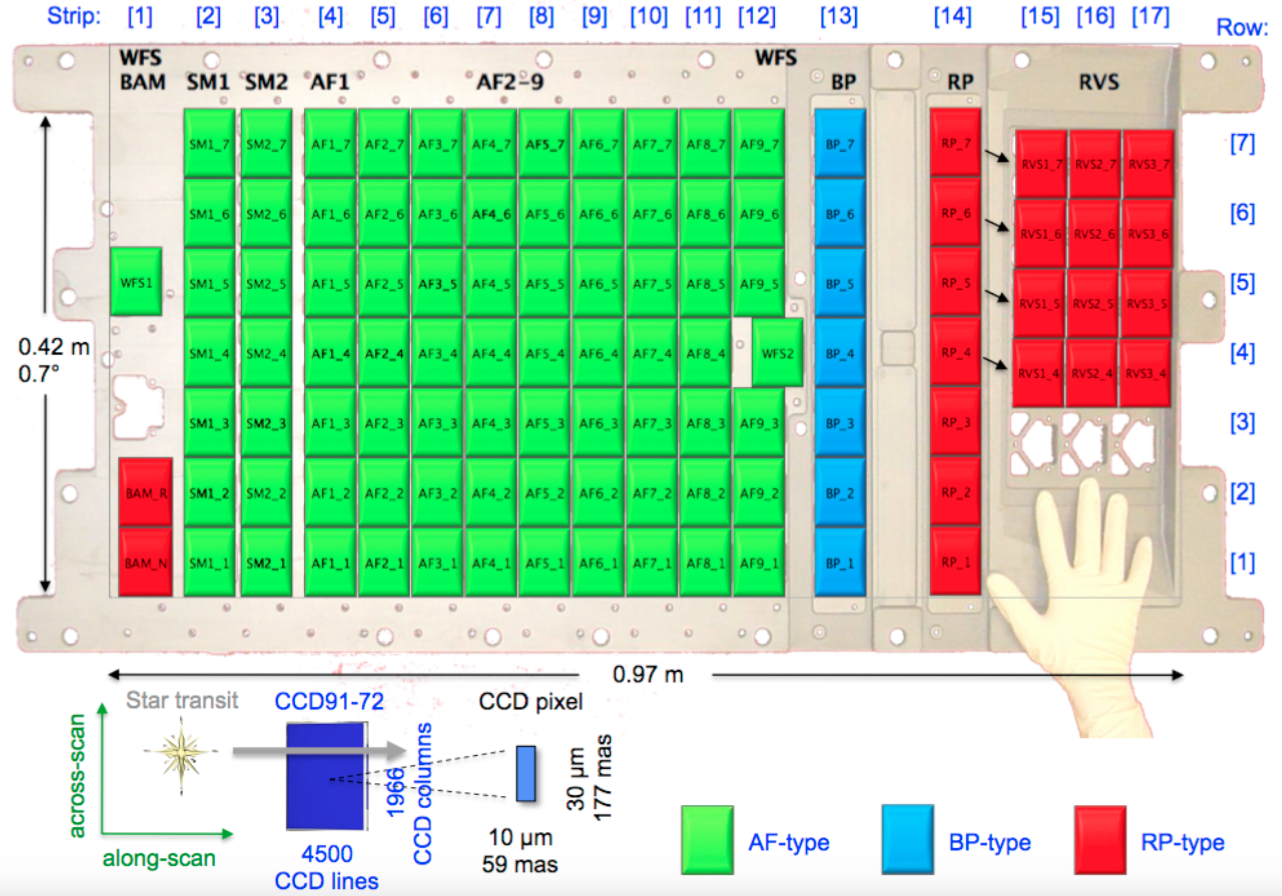
\includegraphics[width=\columnwidth]{gaia_ccd.png}
	\caption{Size comparison and spatial arrangement of the CCD detectors in the Gaia focal plane. Image credit: \citet{2016A&A...595A...1G}.}
	\label{fig:gaia_ccd}
\end{figure}

\section{Gaia}
\label{sec:gaia_data}
Gaia is the one-billion-star surveyor of the European Space Agency (ESA). It has been continuously scanning the sky since July 2014 from its designated location close to the second Lagrange point of the Sun-Earth/Moon system. Gaia’s aim is to map the entire sky,down to magnitude $\sim20.7$, and to collect micro-arcsecond-level astrometry and milli-magnitude-level photometry for the brightest 1,000+ million stars as well as medium-resolution spectroscopy for mainly radial-velocity determination of the brightest subset of $\sim150$ million objects. 

The Gaia scanning of the sky is composed of two independent, superimposed motions: a rotation around the spacecraft spin axis with a period of 6 hours plus a slow, 63 day period precession of the spin axis around the Solar direction at a fixed Solar-aspect angle of $45^\circ$. Over the nominal five-
year mission, Gaia has completed $29$ of these precession periods, leading to an optimally uniform sky coverage with, on average, $\sim70$ astrometric and photometric transits across the focal plane (and $\sim40$ for the spectroscopic instrument). In the extended mission phase that started in July 2019, a similar scanning law is being employed but with a reversed precession direction during the first year. A passage of a star through the focal plane is called a field-of-view transit. During each transit, Gaia collects instantaneous, so-called epoch data of each object. Publication of all epoch data is scheduled (see Table \ref{tab:gaia_drs} for the final data release.

\begin{table}
	\centering
	\caption{Past and future predicted release dates of Gaia data and products.}
	\begin{tabular}{c c}
		\hline
		Release designation & Date \\ 
		\hline
		Gaia DR1 & 14 September 2016 \\
		Gaia DR2 & 25 April 2018 \\
		Gaia EDR3 & 3$^{rd}$ quarter of 2020 \\
		Gaia DR3 & 2$^{nd}$ half of 2021 \\
		Final release & not yet determined \\
		\hline
	\end{tabular}
	\label{tab:gaia_drs}
\end{table}

As the spacecraft slowly rotates, observed stars traverse the Gaia focal plane equipped with 106 CCD detectors (show in Figure \ref{fig:gaia_ccd}). Every star that gets observed therefore passes trough a sequence of those detectors who analyse a star in the given order:

\subsection{Photometry and astrometry}
The first array of CCDs that collects light from stars is a Sky Mapper (SM) that autonomously detect objects. Stars brighter than magnitude $\sim3$ are too bright to be detected automatically. The faint detection threshold is set at $20.7$ magnitude in the Gaia G band but is not infinitely sharp due
to on-the-fly magnitude estimation errors of the on-board software.

After the source detection, stars pass into the largest array of CCDs that is attributed to the Astrometric Field (AF). It collects the instantaneous positions and fluxes of all objects detected by the Sky Mapper as they traverse along the field. Astrometric measurements are made in a white-light bandpass, covering the range from 3300 to 10500 \AA, which is referred to as the Gaia G band.

The last spectro-photometric measurements are thereafter performed by two low dispersion detectors that are measuring precise fluxes in a number of narrow-pass sub-bands of previously mentioned wide-pass G band. The Blue Photometer (BP) collects low resolution spectra of all objects over the wavelength range from 3300 to 6800 \AA. The integrated magnitude is referred to as the G$_{BP}$ or BP magnitude. The Red Photometer (RP) collects low-resolution spectra of all objects over the wavelength range from 6300 to 10500 \AA. The integrated magnitude is referred to as the G$_{RP}$ or RP magnitude.

\subsection{Spectroscopy}
A final measurement performed by the spacecraft is spectroscopy over the whole observed field of the sky. The integral-field Radial Velocity Spectrometer (RVS) \citep{2018A&A...616A...5C} collects medium-resolution spectra (spectral resolving power (R) $\sim11,700$) over the wavelength range from 8450 to 8720 \AA, for all objects brighter than magnitude $\sim16$ in this bandpass. The location of the pass-band is selected to cover the ionised calcium (CaII) triplet with a prominent absorption features over a large temperature range of stars and can therefore be used to determine radial velocity of spectrally diverse stars. The integrated magnitude in the RVS bandpass is referred to as the G$_{RVS}$ magnitude. The RVS has a reduced field of view orthogonal to the scan direction such that fewer observations up to the RVS limiting magnitude are collected compared to photometric fields in a ratio of 4:7.

\section{Gaia DR2}
\label{sec:gaia_dr2_data}
The second data release of Gaia data (Gaia DR2) was heavily used during the production of this thesis, therefore it requires detailed description of provided tables, its use and potential problems. The release set is far from complete and similar to the final release, but on the other hand provides an unprecedented set of homogeneously acquired and reduced stellar informations newer seen before. Visual and numerical representation of the specific stellar product is given in Figure \ref{fig:gaia_drs}. Gaia DR2 is based on data collected by the spacecraft between 25 July 2014 and 23 May 2016, spanning a period of 22 months. 

\begin{figure}
	\centering
	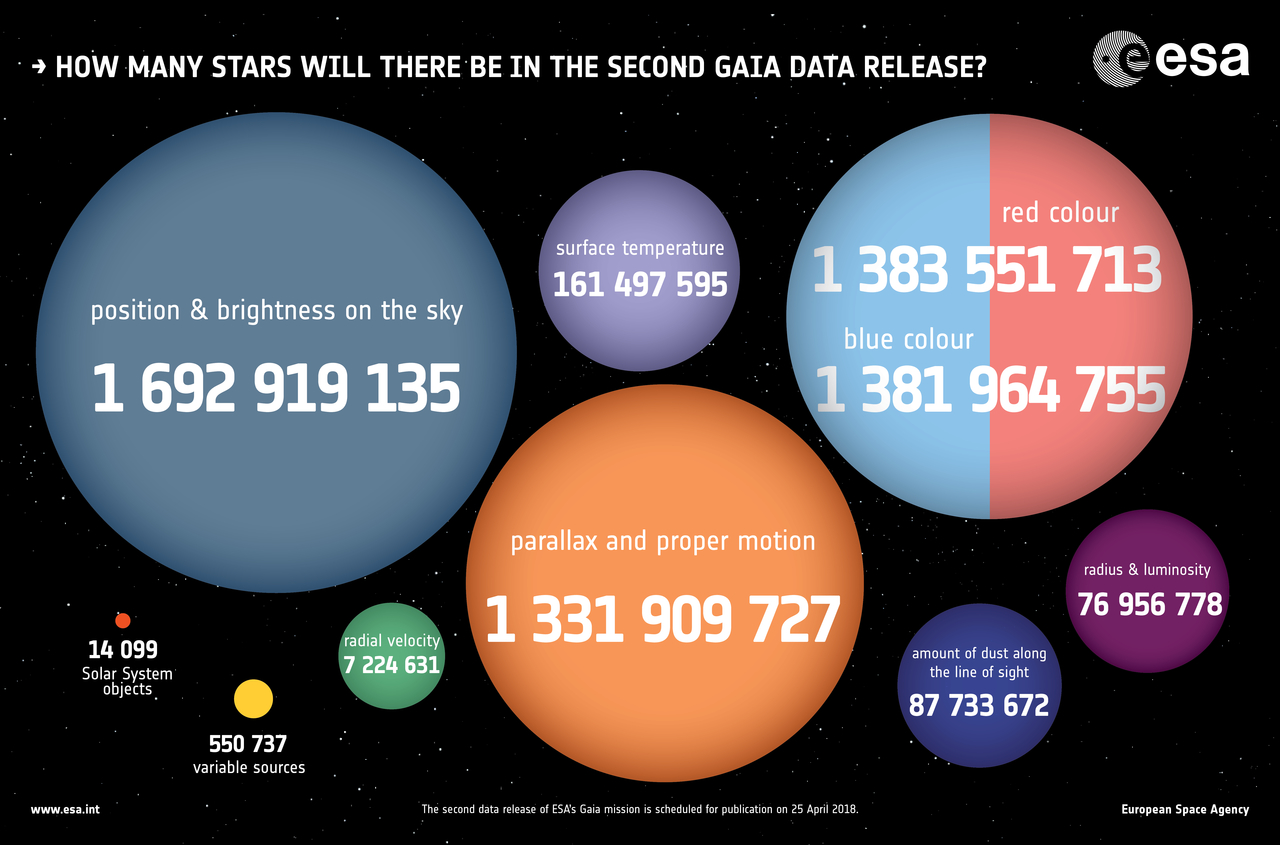
\includegraphics[width=\columnwidth]{1567214817936-Gaia_DR2_numbers_1280.jpg}
	\caption{Visual and numerical representation of Gaia DR2 stellar content. Image credit: ESA, CC BY-SA 3.0 IGO.}
	\label{fig:gaia_drs}
\end{figure}

Along the calibrated raw measurements, Gaia Data Processing and Analysis Consortium (DPAC) provides numerous parameters and properties of stars, pre-selected Solar system bodies and quasars that can be used and explored by users. Among them we can find:
\begin{itemize}
	\item \textbf{Astrometric set} consisting of partial 2-parameter (limited to celestial positions $\alpha$ and $\delta$) and full 5-parameter astrometric solution with addition of including parallax, and proper motion. The 2-parameter sources are typically faint (with about half of them at magnitude G > 20.6), have very few observations (less than five as required for full solution), or very poorly fit the five-parameter astrometric model. All sources fainter than magnitude G = 21 have only positional information. In the current data release all stars are still treated as single during astrometric fit, which could significantly influence solutions in the case of multiple fast moving sources contributing to the position of an observed photocentre. The Gaia coordinate reference frame is aligned with the International Celestial Reference Frame (ICRF) using positions of extragalactic sources such as quasars \citep{2018A&A...616A..14G}. After the initial release, it was determined that the quality of an astrometric fit is best described by the renormalised astrometric chi-square (RUWE) \citep{ruwe}. Further details about astrometric processing and validation are given in \citet{2018A&A...616A...2L, 2018A&A...616A...9L}.
	
	\item \textbf{Photometric data set} contains the broad band photometry in the G, G$_{BP}$, and G$_{RP}$ bands, giving us colour information for Gaia DR2 sources that were observed at least twice. The mean value of the G-band fluxes is reported for all sources while colour information (BP and RP) is available for about 80$\%$ of them.	The integrated colour information suffers from strong systematic effects at the faint end of the survey (G~>~$19$), in crowded regions, and near bright stars. In the case when measured fluxes are inconsistent between the G and the G$_{BP}$ and G$_{RP}$ bands (sum of the later two is significantly larger that G measurement) a warning is raised. A quantitative index of this effect is provided in the numerical form as \textit{flux excess factor}. Further details about processing and photometry validation are given in \citet{2018A&A...616A...4E, 2018A&A...616A...3R}.
	
	\item \textbf{Radial velocity measurements} indicate stellar median radial velocity, averaged over the first 22 months of the observations. Therefore stellar multiplicity and their orbital motion can not be determined from current data. Velocities are provided for sources which are brighter than magnitude 12 in the G$_{RVS}$ photometric band. Because of used set of spectral templates during radial velocity determination, velocities are reported only for stars with effective temperatures in the range between $3550$ and $6900$~K (referring to the effective temperature of a used template and not an actual effective temperature of a star). By the RVS pipeline design, determined absolute radial velocity are limited to $1000$~\kms. The uncertainties of the radial velocities at the faint end depend on stellar effective temperature and range from $1.4$~\kms\ for cooler to $3.6$~\kms\ for hotter stars. The zero-point of the RVS velocities was determined using a comprehensive set of standard stars with numerous dedicated, precise and temporally spread radial velocity measurements \citep{2018A&A...616A...7S}. Further processing details of RVS data are given in \citet{2018A&A...616A...6S}.
	
	\item \textbf{Stellar variability data set} consists of sources that were firmly identified as variable (based on at least two observations of the two Gaia telescopes). The final number still represents only a small subset of the total amount of variables expected in the Gaia survey. The sources were classified into the following nine categories based on their light curves: RR Lyrae (anomalous RRd, RRd, RRab, RRc), long period variables (Mira type and Semi-Regulars), Cepheids (anomalous Cepheids, classical Cepheids, type-II Cepheids), $\delta$ Scuti and SX Phoenicis stars. If a star had 12 or more observations its light curve was analysed in detail. They are designated as specific object studies (SOS) and consist of variables of the type Cepheid
	and RR Lyrae, long period variables, short time scale variables, and rotational modulation variables. Full details on the variable star processing, results and their validation are given in \citet{2018A&A...618A..30H, 2018A&A...618A..58M, 2018A&A...620A.127M, 2019A&A...622A..60C}.
	
	\item \textbf{Astrophysical parameters} derived by the astrophysical parameter inference system in the Gaia data processing (Apsis) include estimates of \Teff\, extinction A$_G$ and reddening E(G$_{BP}$~-~G$_{RP}$), radius, and luminosity for stars brighter than magnitude G~=~17. Values of \Teff\ are reported only over the temperature range between $3000$ and $10,000$~K that is induced by the training set for the algorithm responsible for the \Teff\ estimation. Estimates of the other astrophysical parameters are published for about half of the sources with determined \Teff. As the processing pipeline was performed individually for every object and with a limited set of input data (three Gaia photometric bands and parallax) some errors are expected because of high degeneracy between determined parameters. If a star is located far from expected isochrones used in the processing, extinction becomes overestimated. Full details of the astrophysical parameter processing and result validation are described in \citet{2018A&A...616A...8A}.	
	
	\item \textbf{Solar system objects} (SSO) data set provides epoch astrometry and unfiltered G photometry for a pre-selected list of $14,099$ known minor bodies in the solar system that are numbered in the Minor Planet Center repository. Each time a given SSO enters field of view of Gaia telescopes celestial positions are recorded as seen from the spacecraft. The data set and its production are thoroughly described in \citet{2018A&A...616A..13G}.
	
\end{itemize}

The above sections are partially adapted and summarized from \citet{2016A&A...595A...1G, 2018arXiv180409365G, gaia_primer}.

\section{GALAH}
\label{sec:galah_data}
The GALactic Archaeology with HERMES (GALAH) \citep{2015MNRAS.449.2604D} is an ongoing spectroscopic survey that aims to unveil the Milky Way’s formation history by studying the detailed chemical composition of observed stars. Fossil remnants, which have been disrupted during the formation and are now dispersed around the Galaxy, are tough to have conserved the initial chemical signature of individual galactic components. It is essential to disentangle their formation location and migration history in order to explain current stellar populations. This can be achieved trough the technique of chemical tagging \citep{2002ARA&A..40..487F} that promises identification of old dispersed fossil remnants based on their unique abundance patterns over numerous chemical elements. The GALAH aims to achieve this by measuring up to 31 elemental abundances (from 7 independent element groups with different physical origin) individually in every acquired spectrum.

The GALAH survey was the main driver for the construction of the High Efficiency and Resolution Multi-Element Spectrograph (HERMES) \citep{2010SPIE.7735E..09B, 2015JATIS...1c5002S}, a multi-fibre spectrograph mounted on the $3.9$-metre Anglo-Australian Telescope (AAT) situated at the Siding Spring Observatory, Australia. The spectrograph has a resolving power of R $\sim 28,000$ (or R $\sim 45,000$ when slit mask is used) and covers four separately acquired wavelength ranges (4713 -- 4903~\AA, 5648 -- 5873~\AA, 6478 -- 6737~\AA, and 7585 -- 7887~\AA), together covering approximately 1000~\AA, including the H$\alpha$ and H$\beta$ lines. The ranges are frequently referred to as blue, green, red and near-infrared spectral arms. This configuration can simultaneously record spectra from up to 392 fibres distributed over a $2^\circ$ diameter field of the night sky, with an additional 8 fibres used for the telescope guiding. The spectrograph can typically achieve a signal to noise ratio (SNR) $\sim100$ per resolution element at magnitude V=14 in the red arm during a 1-hour long exposure. 

\subsection{Acquired spectra and target selection}
The spectroscopic data used during the production of this thesis were taken from the pilot survey, the main GALAH survey \citep{2015MNRAS.449.2604D}, the K2-HERMES survey \citep{2018AJ....155...84W}, the TESS-HERMES survey \citep{2018MNRAS.473.2004S}, and special dedicated the HEMRES open clusters (De Silva et al. in preparation) and the HERMES Orion star forming region (Kos et al. in preparation) surveys. Together they form a dataset of $669,845$ successfully reduced stellar spectra, of which a small fraction belongs to a repeated observations. All acquired spectra are homogeneously reduced to one dimensional spectrum, normalised and shifted to stellar reference frame (detailed description in \citet{2017MNRAS.464.1259K}). Combination of those surveys produces increased number of spectra compared to the main GALAH survey, but at the same time breaks rule of a simple unbiased selection function (Sharma et al. in preparation) that is desired for population studies and easier comparison with synthetic galactic models.

The original selection function of the main GALAH survey is separated into two magnitude limited filed selections - bright (10<V<12) and normal (12<V<14) fields whose target selection is colour independent. Used V magnitude is inferred from magnitudes measured by the Two Micron All-Sky Survey (2MASS) \citep{2006AJ....131.1163S} whose photometric bands are shifted into infra-red spectral region. Because of that, some, especially peculiar and variable stars, might have erroneous estimation of V magnitude leading to an underexposure or excessive spectral crosstalk. Because of expected crowding problems (projected diameter of used optical fiber on the sky is equal to $2$\arcsec) observed stars are located at higher Galactic latitudes ($|b|$~>~$10^\circ$) where density of stars is lower. Additional surveys sometimes break those rules by selecting fainter/dimmer stars, going closer to the Galactic plane, employ colour cuts, or favor interesting preselected stars such as K2 \citep{2014PASP..126..398H} targets, TESS \citep{2015JATIS...1a4003R} targets and cluster members. Therefore some care is needed when trying to infer global stellar or galactic properties based on such inhomogeneous selection criteria.

\subsection{Spectral reduction and parameters determination}
Stellar atmospheric parameters and individual elemental abundances derived from normalized spectra, acquired by different surveys, are analysed with the same procedure that slowly evolved and improved during the course of the GALAH survey.

\begin{itemize}
	\item DR1
	\item DR2
	\item DR3
\end{itemize}


adaptation of Spectra Made Easy (SME) \citep{1996A&AS..118..595V, 2017A&A...597A..16P} software that is described in-depth by Buder et al. (in preparation) as part of the latest data release (DR3) of the GALAH spectra and derived parameters.


\section{Asiago}
\label{sec:asiago_data}
Vastly different from the previous two massive all-sky surveys, telescopes at the Asiago site are mainly used for dedicated observations or monitoring of previously selected targets, whose observational and astrophysical potential was identified from all-sky surveys. During our stay at the Asiago observatory, that usually lasted for four consecutive bright nights every month, we used $1.82$~m Copernico telescope located on top of the nearby hill Mount Ekar (Asiago, Italy - altitude of $1,366$~m).

All our observations were performed by the Echelle spectrograph that is mounted on the telescope on days around the full Moon when quality and deepness of photometric observations is heavily reduced. Design of the Echelle instrument and its slit length enables observer to observe only one star a time. Obtained spectra have a resolving power of R$\sim20,000$ and a wide span of wavelengths between $3600$ and $7400$ \AA. They are divided into 30 orders who partially overlap with succeeding and preceding order, providing an undisturbed coverage of observed wavelengths. Acquired spectra are recorded by Andor CCD with the size of $2048 \times 2048$ pixels. This setup enables us to capture spectra of stars with magnitudes V~<~$10$ at high SNR with reasonable exposure time (less than 1 hour per spectrum). Because of the mechanical limitation, observed stars must be positioned at least $15^\circ$ above the local horizon. At those low altitudes, only the brightest stars are reasonable to be observed because of strong atmospheric attenuation.

Combining location of the observatory and above observational limitations with the fact that our interesting stars were selected from the GALAH survey, highly reduces the number of potentially observable objects. To reduce the atmospheric effect effects, we only observed stars which rose at least $30^\circ$ above the local horizon that is equal to having right ascension above $000000^\circ$. As described in more detail below, we used additional Asiago observations to inspect spectroscopic features not accessible by the GALAH spectra and to prolong radial velocity time series of possible multiple stars who could show signs of radial velocity changes not detectable by a single epoch GALAH spectrum.

Additionally to our program observations, we also contributed spectroscopic observations that resulted in published astronomer's telegrams \citep{2019ATel13340....1M} and scientific papers \citep{2019MNRAS.488.5536M}.

\chapter{Chemo-dynamic tracing of open cluster stars}
\label{chap:clusters}
One of the main goals of the \Gh\ survey is to explore possibilities of chemical tagging for random field and known open cluster stars. A task that sounds easy in theory, but its working applications are far from ready for large spectroscopic surveys. The road to getting precise stellar chemical abundances leads around many different obstacles, which all have an impact on the final determined abundance values whose precision and accuracy dictates the possibility and success of implementing chemical tagging.

In this chapter, we present our exploration of abundances for a few open clusters that were observed as part of multiple different surveys served by the HERMES spectrograph. In Section \ref{sec:intro_tag}, we briefly describe the history of open cluster membership, the evolution of clusters, and means to discover these ongoing processes using stellar abundance information only. Of multiple observed open cluster in the GALAH, we focus only on a small subset of them that have the highest number of members (see Section \ref{sec:galah_clusters} for the complete list). Section \ref{sec:membership_v2} describes the selection of clusters and integration of orbits for stars inside and around the clusters. Chemical signature of field and cluster stars is analysed in Section \ref{sec:chem_ej_tag} and the results are summarised and discussed at the end of this chapter.

\section{Introduction}
\label{sec:intro_tag}
The latest second release of \G\ data (\Gs, \cite{2018A&A...616A...1G}) revolutionized numerous fields of astronomy, including research of galactic open clusters. Its combined information of stellar distance, kinematics, and photometric measurements enables us to go beyond simple methodologies, such as star density counts, to unravel even the faintest and sparsest components of open clusters. So far, many works have been published trying to refine parameters, and membership information of long known open clusters \cite{2017A&A...601A..19G, 2018A&A...618A..93C, 2019A&A...627A..35C} and find new, less numerous or fainter clusters \cite{2019ApJS..245...32L, 2019JKAS...52..145S, 2019A&A...624A.126C, 2020arXiv200107122C}. Such thorough and the improved investigation uncovered that many of the clusters listed in modern catalogues, initially discovered as apparent stellar overdensities, are no more than chance alignments of stars and not true physical clusters \cite{1998A&A...340..402B, 2000A&A...357..145C, 2016AJ....152....7H, 2018MNRAS.480.5242K, 2020A&A...633A..99C}.

Born from the same molecular cloud, open clusters are ideal test structures for different astrophysical principles. Being influenced by external and internal processes, such as tidal stripping and close stellar interactions, their lifetime is limited from about 100 Myr to a few Gyr for the densest structures \cite{1998A&A...337..363P, 2013MNRAS.434.2509M}. This gives us a possibility of observing them at different evolutionary stages \cite{2006BASI...34..153C, 2007A&A...468..139P} before they blend \cite{2001A&A...366..827B} into field stellar population. The most prominent transitional features we can observe are compact cluster tidal tails \cite{2019AA...627A...4R, 2019AJ....157..115Y, 2019AA...621L...3M, 2019arXiv191206657Z} and lose extended halos of evaporated stars. They are observed as a slowly decreasing over-density \cite{2002A&A...385..471C, 2004A&A...427..485B, 2019AA...627A.119C} of stars far from a denser cluster core. Due to close gravitational interactions among members, they can be ejected out of a cluster at high velocities \cite{2009MNRAS.396..570G, 2010MNRAS.402..105G, 2017MNRAS.470.3049R}. Such cluster members can on the sky be found several degrees or even further away from their main cluster body \cite{2007MNRAS.376L..29G, 2018MNRAS.473.4612K, 2019ApJ...884....6M}. Identification of such stars could be done using a chemical tagging procedure, whose importance and potential problems have already been discuses in Section \ref{sec:open_clustesr_tagging}. 

\section{Additional data specifics}
\label{sec:data_clusters}

\subsection{The GALAH and cluster stars}
\label{sec:galah_clusters}
Among the dedicated HERMES cluster observations and other HERMES surveys, such as the main \Gh\ survey, we detected members of known open clusters, whose stellar membership was taken from results published by \citet{2018A&A...618A..93C}. Their clustering methodology relies on the unsupervised membership assignment code called Unsupervised Photometric Membership Assignment in Stellar Clusters (UPMASK, \cite{2014A&A...561A..57K}). Initially, the methodology was designed to find overdensities using only stellar position and photometry. As the methodology is unsupervised and has zero knowledge about physics or input data, \citet{2014A&A...561A..57K} easily applied it to work with astrometric and positional data. Internally UPMASK creates many incarnations of random values from the input data and their uncertainties, selects the four most important principal components, and runs the clustering algorithm on the components. At the end, detected overdensities are compared with random stellar fields and overdensities of the last iteration. Membership probabilities depend on how often a star was inside the relevant overdensity.

As some of the clusters were not targeted intentionally by the surveys or only their cores, the number of observed members and surrounding field stars of interest can vary substantially. The clusters analysed in this paper, having the most significant number of spectroscopic observations are Berkeley 32, NGC 2516, NGC 2112, NGC 6253, Blanco 1, Ruprecht 147, NGC 2632, NGC 2682,  Melotte 22, and Collinder 261. To supplement their selection, we added members of Melotte 25 cluster whose membership selection was performed by us as it was missing in the mentioned published paper \cite{2018A&A...618A..93C}. The first step of our methodology was comparable to UPMASK. Similarly, we generated many incarnations of the data to determine the kinematics of a cluster. It was computed as a median proper motion of the over-density that was closest to the previously known centre at every iteration. After selection in proper motion space, we used the same stars to determine clusters centre in position, distance, and radial velocity. A multivariate Gaussian distribution was fitted at the determined parameter to assess membership probabilities.

\subsection{Gaia}
\label{sec:gaia_clusters}
For a complete 6D positional and kinematics stellar information, we augmented the \Gh\ data with proper motion, parallax and radial velocity from the \Gs\ data-set. As all investigated open cluster stars are located close to the Sun, their distances can be inferred by the inversion of a parallax value ($1 / \varpi$). Of course, we could, at this point, use a bit more accurate distances that were determined using distance priors based on a Galaxy model \cite{2018AJ....156...58B}. The second approach does give more reliable and symmetric distance uncertainties, but does not reduce the elongated shape of stellar clusters (in radial direction away from our location in the Galaxy) as the distance to every star is determined individually. At the same time, more distant stars have grater relative parallax uncertainties which makes it even more difficult to determine distance and shape of a cluster. To get a more realistic shape of a cluster, all member distances would have to analysed at the same time with inclusion of the isochrone information.

The current release of the \G\ data contains magnitude limited range of recovered radial velocities, that are, whenever possible, supplemented or substituted with the \Gh\ measurements of higher accuracy \cite{2018arXiv180406344Z}. Supplemented are mostly stars fainter than currently adopted \G\ RVS \cite{2018A&A...616A...5C} analysis threshold as the GALAH targets are much fainter stars than the RVS limit. The synergy, therefore, increases the set of useful stars in our case.

\section{Cluster and field members}
\label{sec:membership_v2}
The first step in our analysis was the acquisition of data relevant for each cluster identified among the \Gh\ observations. Identification of observed clusters was made by matching observed stars with known cluster members published by \citet{2018A&A...618A..93C}. As some of the clusters had a low number of stars or were proved to be chance alignments of stars \cite{2018MNRAS.480.5242K}, they were not considered in the analysis. Sky coordinates and distances of selected open cluster members (see Section \ref{sec:galah_clusters} for the list of considered clusters) were taken from \citet{2018A&A...618A..93C} and served us as anchors around which we queried the \Gs\ data. A cone query with a radius of $6^\circ$ and distance limit of $\pm900$~pc around a cluster centre was performed to download a subset of the whole dataset. The elongated shape of queried dataset volume is a result of clusters' apparent elongated shape. A bit different volume was used for a nearby and visually extensive cluster Melotte 25, for which we used radius of $12^\circ$ and distance limit of $\pm200$~pc around its centre. 

The downloaded subset included stars with an incomplete set of \G\ parameters. To complement and improve quality of radial velocity measurements, all available \Gh\ velocity estimates in a subset were used to override or supplement \G\ measurements. In the case of multiple \Gh\ observations, a median velocity per star was used. 

The initial open cluster memberships were taken from \citet{2018A&A...618A..93C} but needed some refinement before it was suitable for us. To select as many possible cluster members, the employed membership algorithm did not relay on magnitude limited radial velocity information to assign cluster membership. To make cluster volume more compact and retain only the most probable core members, we discarded all member stars whose radial velocity deviated for more than $5$~\kms\ from the cluster median value of all retrieved members. The used threshold was determined empirically by observing velocity distributions to discard only a few of the most dissimilar stars. The reason behind this velocity limitation will be evident in Section \ref{sec:orbit_tracing} where we try to keep the cluster volume as compact as possible during its integration. This thresholding prevents unwanted pollution of a cluster by field stars during comparison of their chemical signatures in Section \ref{sec:chem_cluster}. 

\subsection{Stellar tracing}
\label{sec:orbit_tracing}
After the selection of open cluster members, we proceeded with the analysis of stellar movements inside and outside the cluster. In order to get the most reliable motion information, only stars with a complete 6D kinematic information (proper motion + radial velocity + sky coordinate + parallax) were considered. No additional \G\ quality flagging was used to remove stars with potentially wrong parameter estimates as we would like to show in the following steps that they could be discovered and eliminated based solely on their chemical composition.

By knowing members of the observed clusters, their current position, and complete motion vectors, we can trace the path of a volume constrained by the cluster stars backwards or forwards in time. This integration procedure was performed by individual integration of cluster stars in axisymmetric gravitational potential (\textit{MWPotential2014} potential described by \citet{2015ApJS..216...29B}) using \GP\ software library version 1.5.0. \cite{2015ApJS..216...29B}. Being interested in the past ejected members of a cluster, we integrated orbits of cluster stars for $120$~Myr (comparable to ages of the youngest open clusters in our set) into their past and saved their location after every step of $20$~kyr. As the integration process relies only on the present uncertain measurements of their velocities and distance, longer integration is not precise or reliable. This uncertainty is observed by the fact that the cluster volume gets larger during backwards integration instead of staying approximately constant as it would in the case of gravitationally bound stellar components. The volume could also keep shrinking during backwards integration if cluster is loosely bound and is already slowly dissipating at the present time. At every integration step, the cluster volume was described by a minimum convex hull defined by its outer-most members. They serve as vertex points of the constructed geometric body. Such a geometrical shape presents the smallest bounding volume with partially flat boundaries which encompasses all considered members.

The next step of our analysis consisted of finding stars in the clusters' immediate neighbourhood that could be traced back to having origin inside the considered open cluster. To filter-out field stars that travel into a completely different direction than the cluster, we discarded all stars whose galactic velocity vector difference towards present cluster velocity vector was >$50$~\kms. This threshold, therefore, defines the fastest possible speed at which stars could have been ejected. Orbits of the remaining set of stars (usually more than half of the queried stars) were integrated using the same configuration as cluster stars described above. At this point, we could investigate which orbit of the field stars crosses clusters' volume at any given integration step.

To get a more descriptive crossing probability, we created $250$ incarnations of every field star. Initial kinematic properties of each incarnation were drawn from the Gaussian distributions of parallax, radial velocity, and proper motion defined by their reported values and uncertainties. After analysing all $250$ orbits of each star, we described its cluster crossing probability by the longest stay inside the cluster volume and  by the percentage of crossing events. For a crossing to be counted as confirmed, a star had to be located inside the cluster volume for at least $0.4$~Myr -- time that is equivalent to $20$ integration steps. The final selection of probable ejected stars consist of stars, whose integration procedure revealed that they were crossing a cluster volume in at least $68$\% of the incarnations and their longest stay there was at least $1$~Myr. Remaining volume crossing stars, that did not meet the criteria, were considered as random field stars. They were also discarded from further analysis as they might, in the case they were real past cluster members, additionally pollute chemical signature of the field population. Summary of investigated and discovered stars for every cluster is given in Table \ref{tab:cluster_stats}.

\begin{table}
	\centering
	\caption{Clusters statistics. Only stars with a complete 6D positional and kinematic information were considered for this statistics and orbit integration analysis. Numbers in columns successively present: number of all stars with complete information, number of analysed stars that meet initial criteria of having the galactic velocity similar to a cluster ($\Delta$v~<~50~\kms), number of stars that do not cross cluster volume during integration, number of possibly ejected stars, and number of cluster members that defined volume of a cluster.}
	\begin{tabular}{l c c c c c }
		\hline
		Cluster & Queried from & Analysed & Field & Possibly & Known \\
		 & \G\ DR2 & stars & stars & ejected & members \\
		\hline \hline
		Berkeley 32  & 11322 & 2659 & 2047 & 125 & 23 \\ 
		Blanco 1     & 5043 & 2734 & 2687 & 15 & 81 \\
		IC 4665      & 15022 & 10155 & 9823 & 26 & 34 \\
		Mamajek 4    & 21776 & 11623 & 10513 & 85 & 48 \\
		Melotte 22   & 9097 & 6335 & 5944 & 105 & 239 \\
		Melotte 25   & 6836 & 3782 & 3511 & 165 & 126 \\
		NGC 1817     & 12826 & 4489 & 4060 & 74 & 54 \\
		NGC 1901     & 12666 & 7323 & 7204 & 19 & 30 \\
		NGC 2112     & 13866 & 6665 & 6323 & 38 & 49 \\
		NGC 2204     & 4314 & 1777 & 1170 & 180 & 59 \\
		NGC 2516     & 17383 & 11906 & 11030 & 315 & 182 \\
		NGC 2548     & 14371 & 9212 & 8842 & 60 & 34 \\
		NGC 2632     & 9951 & 5290 & 4991 & 170 & 222 \\
		NGC 2682     & 10947 & 5244 & 4776 & 226 & 287 \\
		NGC 6253     & 62975 & 30114 & 17267 & 1362 & 64 \\
		Ruprecht 147 & 17749 & 5062 & 4850 & 23 & 103 \\
		\hline
	\end{tabular}
	\label{tab:cluster_stats}
\end{table}

\section{Chemical signature of clusters}
\label{sec:chem_cluster}
After defining potential members of different cluster components (field, ejected, and members), we can look into the abundance signatures of an individual component and their overlap. Of all 30 possible \Gh\ chemical abundances, we initially excluded only Li because of its intrinsic variability that depends on the stellar evolutionary stage. Scatters plots of all considered abundances and \Feh\ as a function of \Teff\ for clusters most populated by the \Gh\ data are shown in Figures \ref{fig:ct_cluster1}, \ref{fig:ct_cluster2}, \ref{fig:ct_cluster3}, and \ref{fig:ct_cluster4}. Not all plots for the same cluster have the equal number of points as reporting of abundance values depends on the estimation of their reliable detectability that is based on equivalent widths of elemental absorption lines (thoroughly described in \citet{buder2020}). The plots show only stars with unflagged (\texttt{flag\_sp} = 0, other flag values are described in \citet{buder2020}) stellar parameters, that are presumably of the highest quality.

\begin{figure}
	\centering
	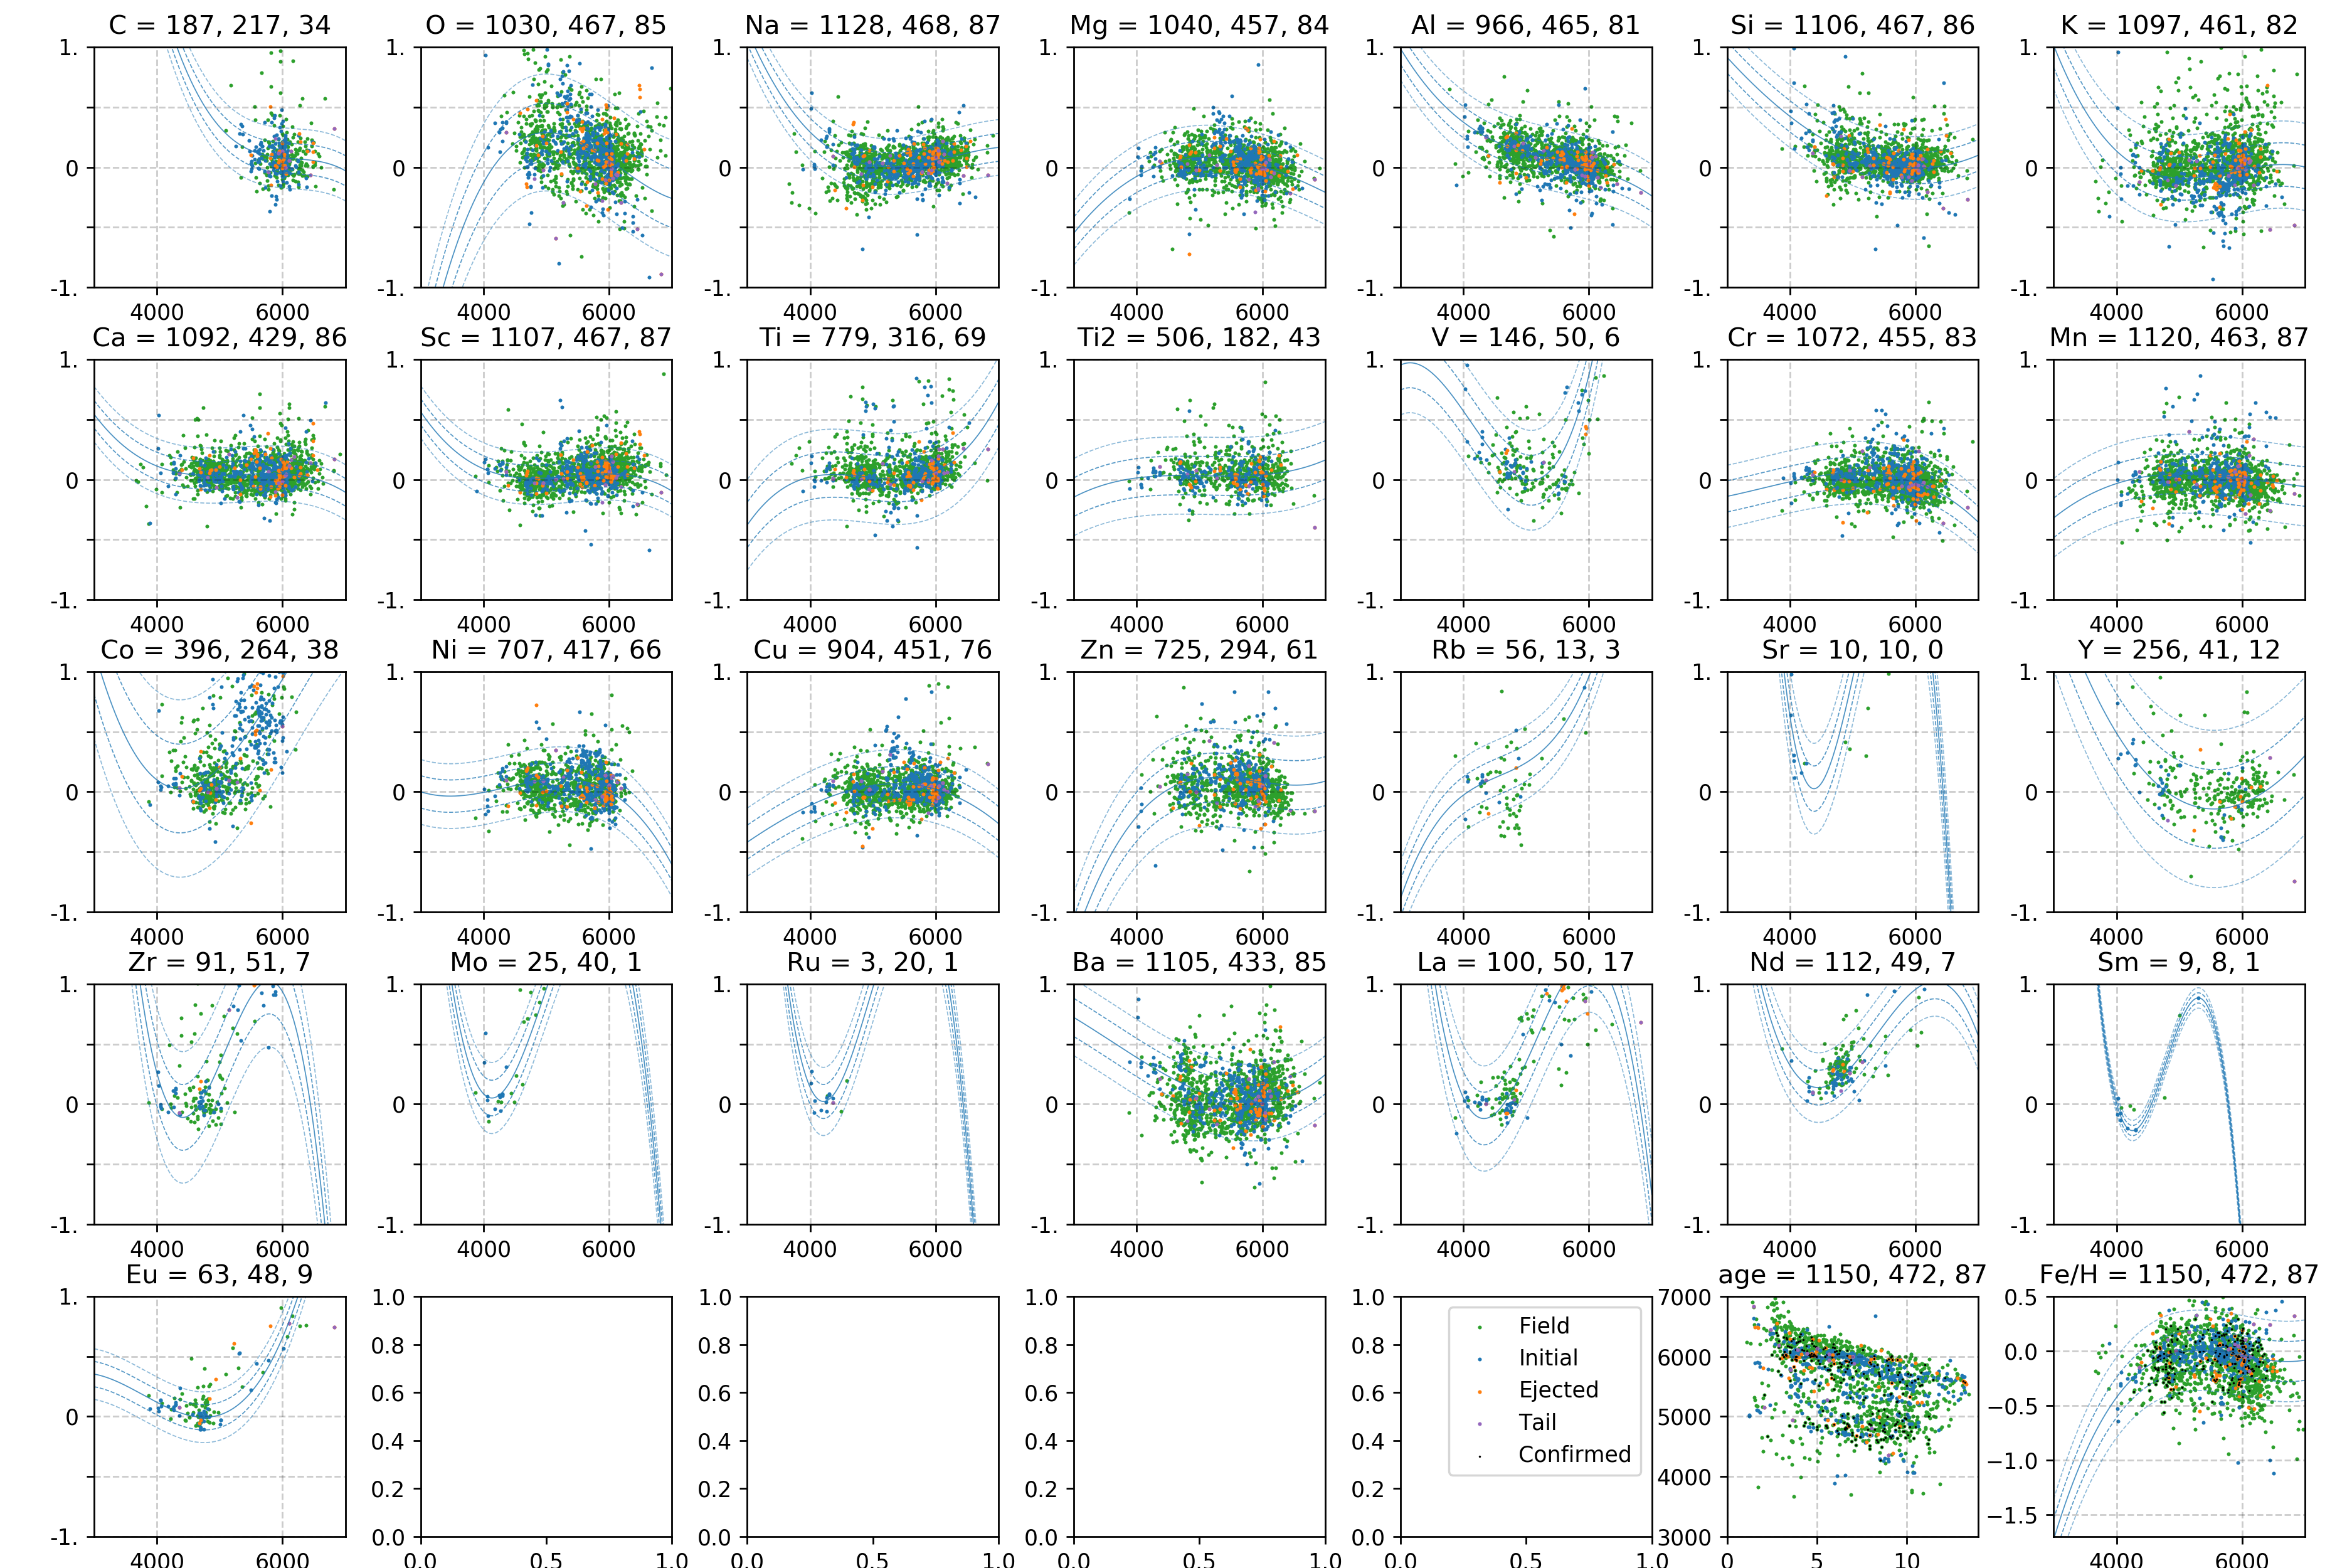
\includegraphics[width=\textwidth]{p_teff_abundances_NGC_2682_orbits_DR3_new_flag0.png}
	\caption{NGC 2632 abundance scatter plots as a function of effective stellar temperature. The solid blue line represents the best fit on the cluster population. The 1$\sigma$ and 2$\sigma$ abundance deviations from the fit are given by dashed blue lines of decreasing intensity. Coloured dots represent field (green), members (blue), and possibly ejected (orange) stars. Their numbers are given above every panel, following the elements' name. Purple dots preset known tails (described later in Section \ref{sec:tails_chem}) of slowly evaporating stars in some clusters. The last two panels present \Teff\ of stars at different ages (in Gyr), and dependence of \Feh\ on their \Teff. The black dots in those two panels indicate possibly ejected stars whose chemistry was matched to cluster stars.}
	\label{fig:ct_cluster1}
\end{figure}

\begin{figure}
	\centering
	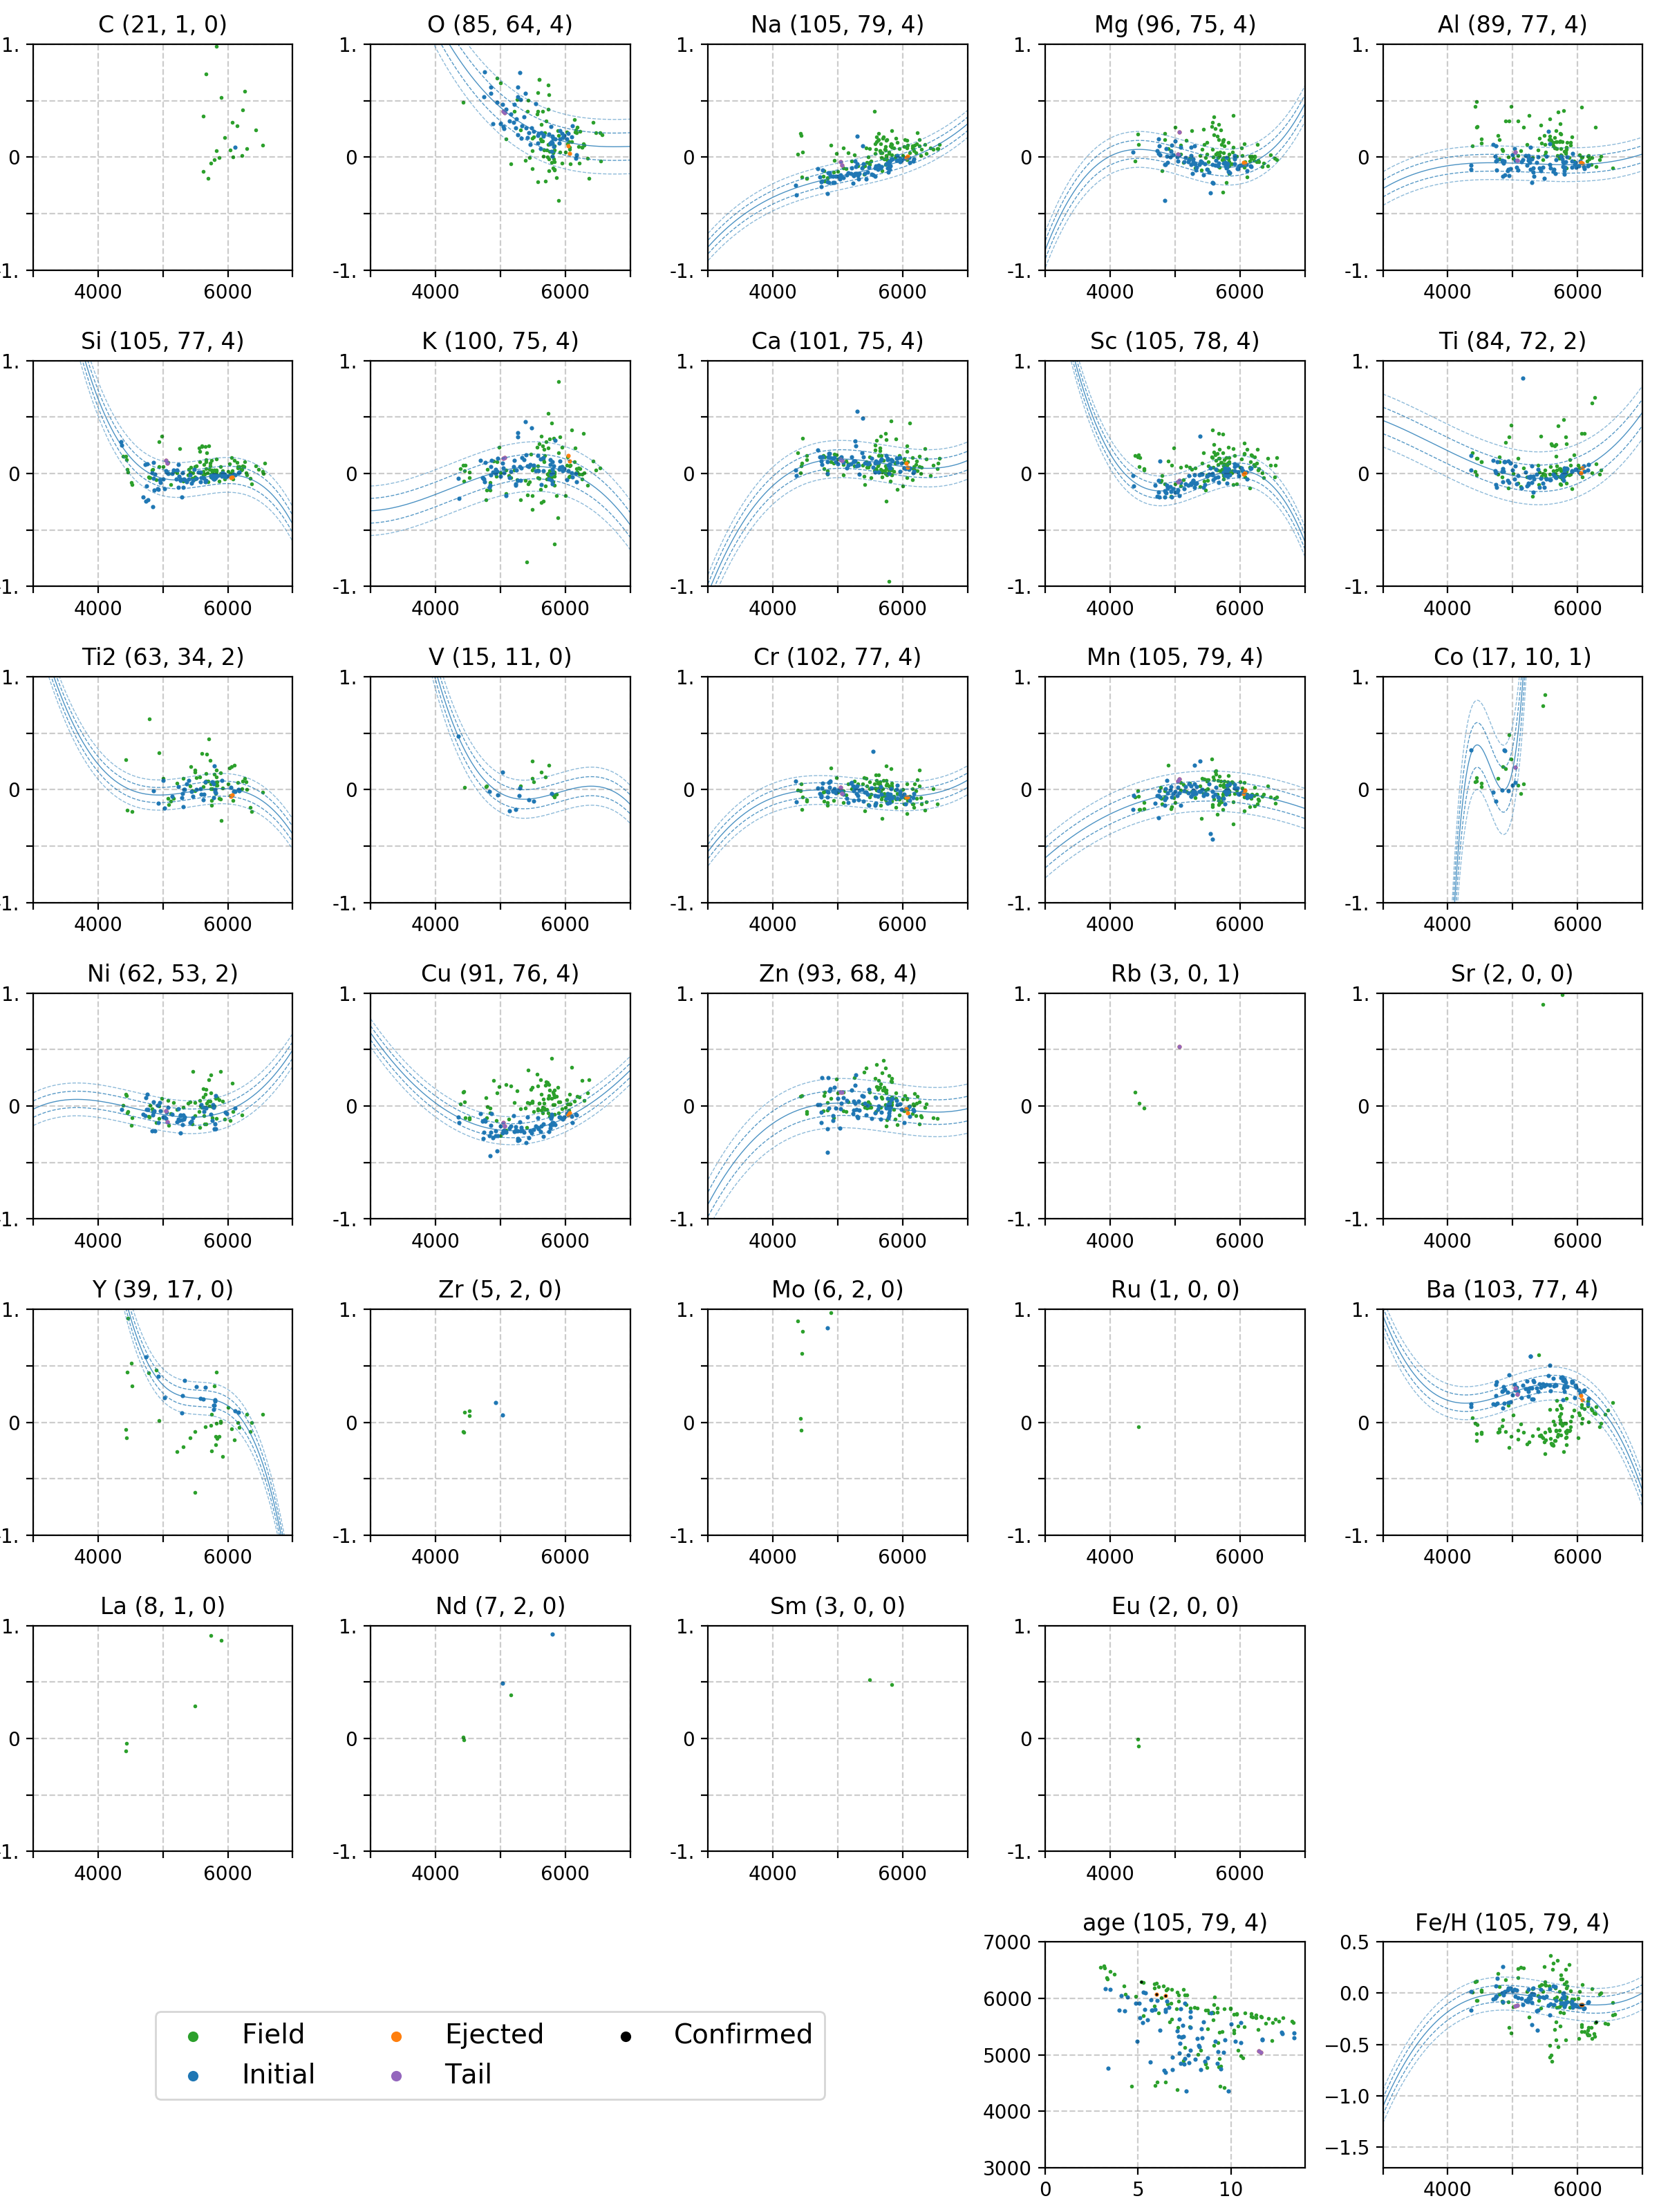
\includegraphics[width=\textwidth]{p_teff_abundances_Blanco_1_orbits_DR3_new_flag0.png}
	\caption{Same plots as in Figure \ref{fig:ct_cluster1} but for open cluster Blanco 1.}
	\label{fig:ct_cluster2}
\end{figure}

\begin{figure}
	\centering
	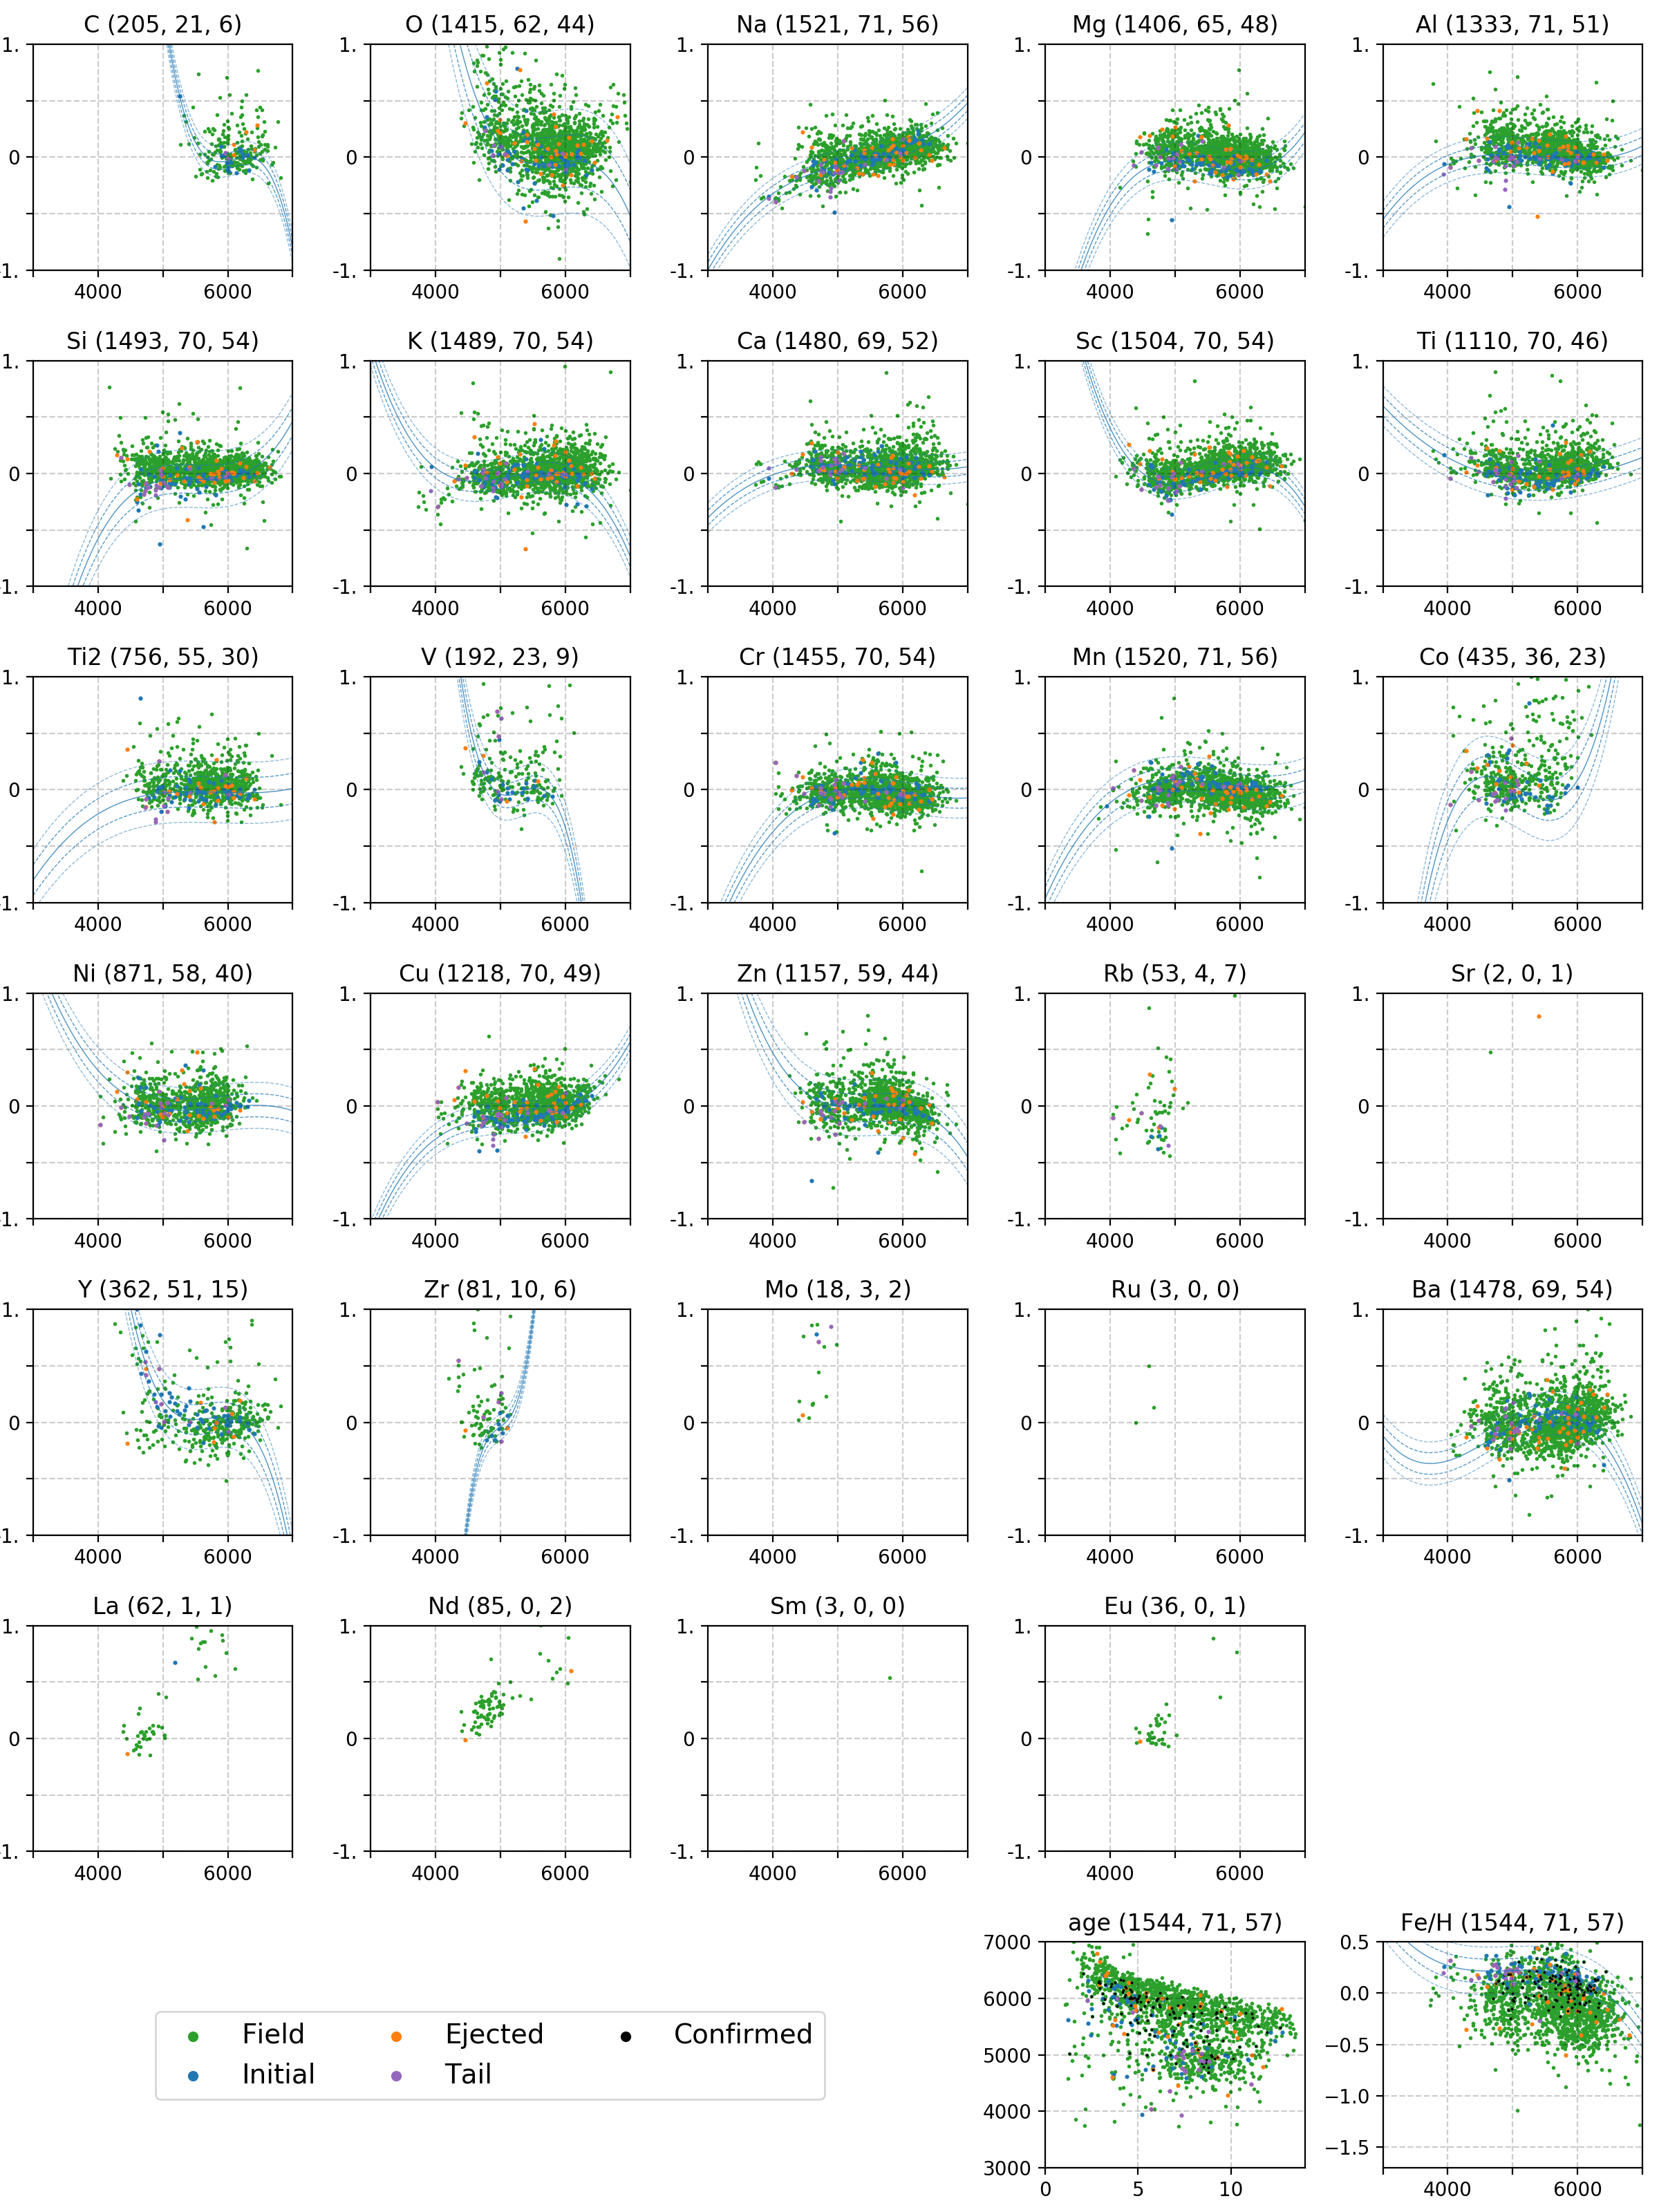
\includegraphics[width=\textwidth]{p_teff_abundances_NGC_2632_orbits_DR3_new_flag0.png}
	\caption{Same plots as in Figure \ref{fig:ct_cluster1} but for open cluster NGC 2632.}
	\label{fig:ct_cluster3}
\end{figure}

\begin{figure}
	\centering
	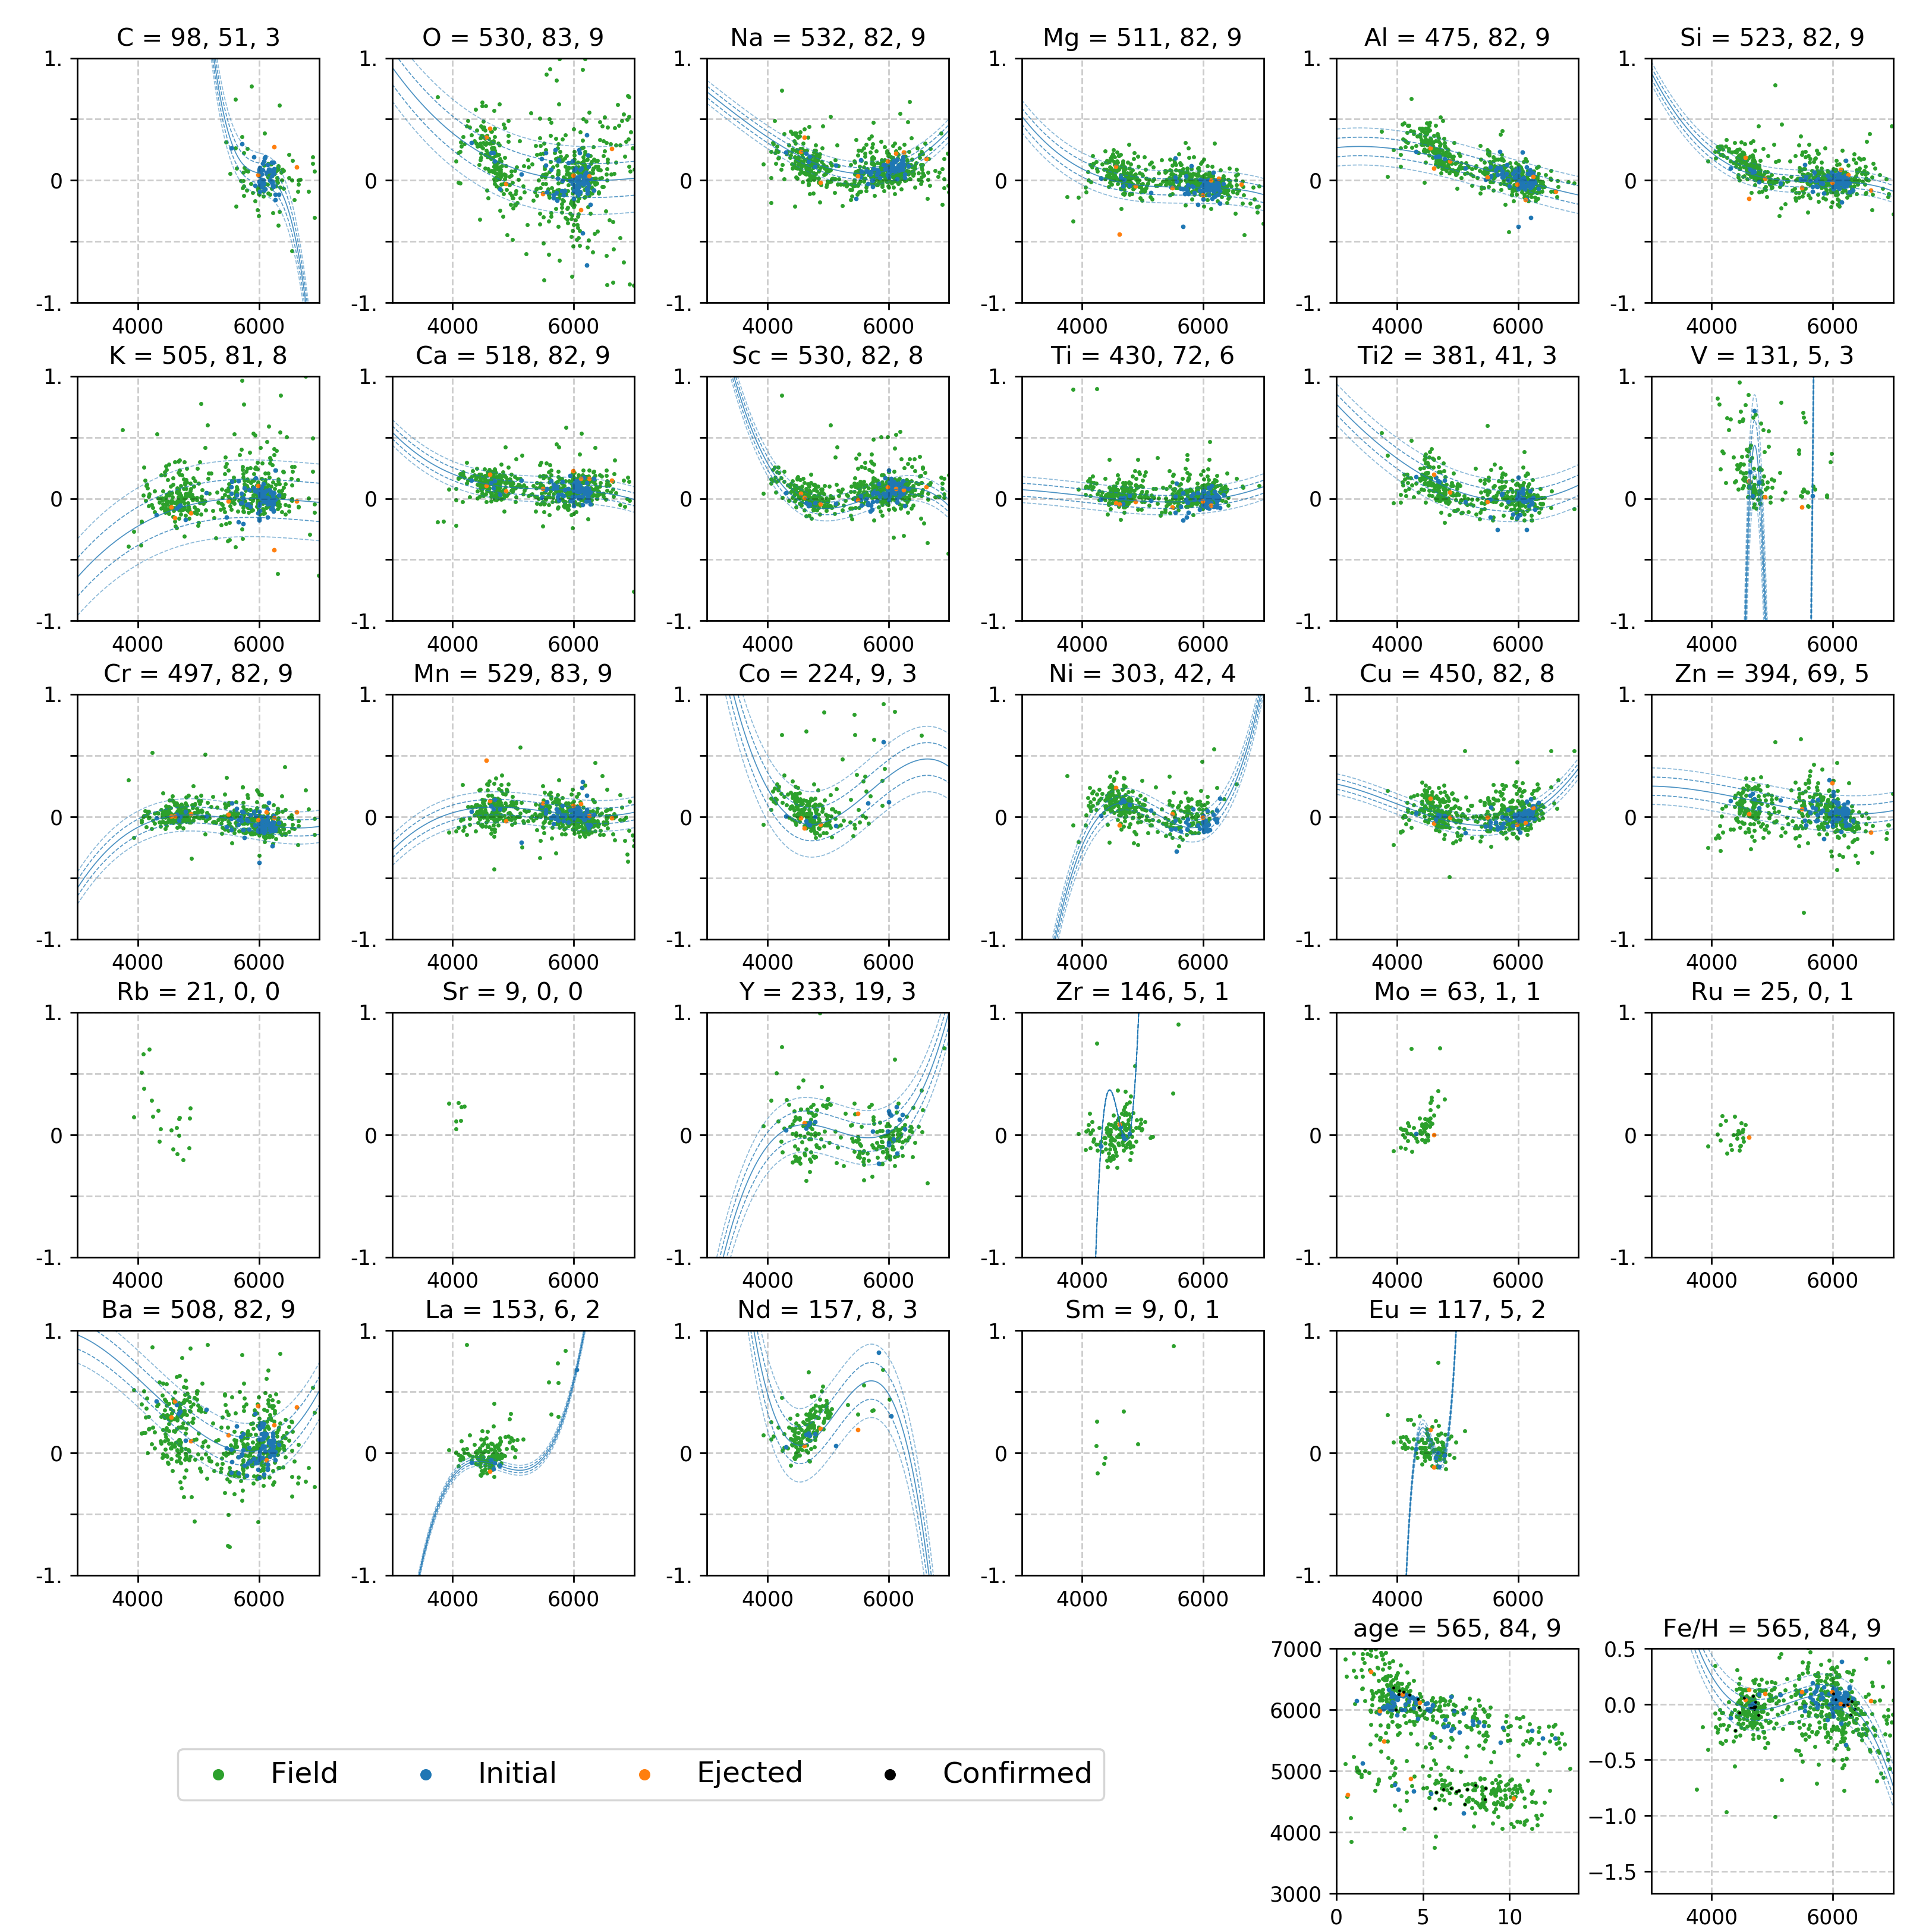
\includegraphics[width=\textwidth]{p_teff_abundances_Ruprecht_147_orbits_DR3_new_flag0.png}
	\caption{Same plots as in Figure \ref{fig:ct_cluster1} but for open cluster Ruprecht 147.}
	\label{fig:ct_cluster4}
\end{figure}

\begin{table}
	\centering
	\caption{The number of acquired \Gh\ spectra among different cluster components that were considered during the chemical comparison. No parameter or abundance flagging was yet used at this point. Stars represented by these statistics are a subset of stars given in Table \ref{tab:cluster_stats}. Because of a small percentage of repeated observations, few clusters (especially NGC 2682 that was used as the calibration and verification field) can have a higher number of spectra than the number of member stars.}
	\begin{tabular}{l c c c }
		\hline
		Cluster & Field & Ejected & Members \\
		\hline \hline
		Berkeley 32  & 42 & 2 & 36 \\ 
		Blanco 1     & 151 & 10 & 109 \\
		IC 4665      & 1114 & 6 & 26 \\
		Mamajek 4    & 2907 & 26 & 13 \\
		Melotte 22   & 1016 & 21 & 67 \\
		Melotte 25   & 653 & 27 & 64 \\
		NGC 1817     & 569 & 11 & 36 \\
		NGC 1901     & 6963 & 19 & 28 \\
		NGC 2112     & 401 & 4 & 66 \\
		NGC 2204     & 129 & 23 & 58 \\
		NGC 2516     & 4604 & 101 & 48 \\
		NGC 2548     & 767 & 6 & 18 \\
		NGC 2632     & 2266 & 77 & 116 \\
		NGC 2682     & 1710 & 147 & 1000 \\
		NGC 6253     & 825 & 34 & 86 \\
		Ruprecht 147 & 798 & 14 & 175 \\
		\hline
	\end{tabular}
	\label{tab:cluster_stats_abund}
\end{table}

\subsection{Abundance and age trends}
\label{sec:abund_trends}
%Ker vidimo in tudi drugi modeli kar mocne trende zastopanosti v odvisnosti od fizikalnih parametrov zvezd, je treba te nekako spraviti na isto raven. Najlazje diferencialno - naredimo fit na kopico in gledamo koliko ostali odstopajo od tega
One of the first things we noticed on the shown abundance scatter plots is their strong dependence on physical parameters, especially \Teff. As this is not the first or unique observation of those trends \cite{2010A&A...523A..71G, 2013ApJ...775...58B, 2016MNRAS.457.3934L, 2018A&A...619A.176B, 2019arXiv191208539C}, they are most likely products of insufficient/inaccurate stellar models and/or actual abundance patterns, and not induced solemnly by the employed \SME\ spectrum analysis pipeline that was used by \citet{buder2020} to determine stellar abundances.

If we presume that observed trends are artificially induced and considered cluster members should have a homogeneous chemical composition that is independent of stellar type, a differential chemical tagging analysis can be used \cite{2019arXiv191208539C}. Such analysis considers only comparisons among stars with a similar set of stellar parameters. To describe observed trends, we independently fitted a 3$^{rd}$ degree polynomial function using $2.5\sigma$ clipping algorithm in 2 steps to every abundance versus \Teff\ diagram. By subtracting fitted trends, we estimated degree of intracluster scatter for every element. Because of limitations of measuring certain abundances, the fit was not performed if the number of valid abundance measurements was lower or equal to a used polynomial degree $+1$.

In the ideal case, all of the trends for the same element observed in different open clusters would have the same shape and would be distinguished only by their abundance offsets that result from their distinct chemical pattern. Looking at our fitted trends, everything is not so simple and easy as the fitted curves can have significantly different shapes. For example, trends of elements Ba and Cu are in general U-shaped. Therefore the highest or lowest abundance values are present in the middle of the \Teff\ region. Those results imply that using the latest \Gh\ abundances, we can not easily find the global behaviour of measured elements. Blindly using the wrong trend line would, therefore completely change results in our case.

Additional identification that there might something be wrong with the parameters lies in the determined ages of individual stars in the clusters. The ages are determined by the best fitting isochrone with appropriate stellar \Feh\ that lies closest to the stars' position on H-R diagram (further details in \citet{buder2020}). As the procedure is run independently for every star in the survey, ages among cluster stars (see plots in Figures \ref{fig:ct_cluster1}, \ref{fig:ct_cluster2}, \ref{fig:ct_cluster3}, and \ref{fig:ct_cluster4}) are strewn over a range of 5~Gyr or more. Fortunately the abundance computation does not require information about the stellar age, but they both share the requirement for an accurate information about the basic stellar parameters.

% TODO Fino bi bilo (morda tudi na grafu) nekako označiti privzeto starost te kopice. Starost ima gotovo tudi precejšnje napake - najbrž je najbolj točna za MSTO (če jih imaš že kaj), pa morda tudi za hladne, ki se šele usedajo na MS. Komentarji tega tipa sodijo v glavni tekst, tu le omeniš, da so tam.

\subsection{Determining chemical similarity}
\label{sec:chem_ej_tag}
%Pogledamo trende in fite, ter koliko moznih izvzenih zvezd se poraja in sklada s temi kemicnimi trendi. Morda nek threshold koliko je dobrih oziroma skladnih s samo kopico, saj ima tudi ta le kar nekaj razpona v izmerjenih/izracunanih vrednostih parametrov.
Having an analytical description of an individual abundance behaviour for every cluster, we can estimate how many and how accurately do the identified ejected stars match with cluster abundance patterns and trends. The most straightforward way to perform this is to count how often does abundance value of an investigated star fall inside a $1\sigma$ (or $2\sigma$ for a more relaxed selection) region around an abundance trend. Both regions and fitted trends are visualised in Figures \ref{fig:ct_cluster1}, \ref{fig:ct_cluster2}, \ref{fig:ct_cluster3}, and \ref{fig:ct_cluster4}. Before performing such counting, we additionally omitted abundance trends of the following chemical elements: V, Rb, Sr, Y, Zr, Mo, Ru, La, and Sm. Their low number of successful measurements per cluster and uncertain trends were not beneficial to the whole chemical tagging experiment and influenced only a small fraction of stars. In general it is not advised to reduce the dimensionality of chemical space for greater differentiation between chemical signatures. As this was one of the first experiments analysing whether the latest \Gh\ DR3 abundances could be used for cluster and global blind tagging, we tried to remove as many additional systematic effects of uncertain measurements as possible. In our case, an individual star was counted as chemically similar if it matched (e.g. fell inside selected $\sigma$ region around the fitted trend line) to a cluster in at least $68$\% of the considered abundances with valid trend fit. Chemically similarity of ejected stars, given as percentage of tagged stars, is presented in Table \ref{tab:cluster_stats_abundtag}.

% TODO To je ok za tabelo 3.3. Morda pa bi v diskusiji tabele 3.3 bilo smiselno pogledati, kako se obnašajo posamezni elementi, recimo ali so še kakšni poleg V, Rb, Sr,... ki zganjajo probleme. Morda tudi, v katere skupine sodijo: a se recimo vsi slow-r elementi obnašajo podobno ali ne. Če se odločiš iti po tej poti, je potem to o različnih kanalih nastajanja elementov dati v uvodna poglavja.

\subsection{Tagging remaining field stars}
\label{sec:chem_fi_tag}
%Kaj se zgodi ce iste kemicne informacije in thresholde uporabimo se za ostale analizirane zvezde v bljizini. Dobimo sploh kaj zvezd ven iz tega in kaksen bi bil v tem primeru njihov kinematicni vektor.
The same principle can also be applied to remaining nearby field stars. As clearly evident from Figures \ref{fig:ct_cluster1}, \ref{fig:ct_cluster2}, \ref{fig:ct_cluster3}, and \ref{fig:ct_cluster4}, the cluster abundances are mostly similar to field stars and lie close to their densest regions in shown abundance scatter plots. Therefore, we were interested in the probability of a random field star being chemically similar to a nearby open cluster. In contrast, some of the investigated clusters, especially Blanco 1, show evident signs of being chemically separable from neighbouring stellar populations. Elements crucial for the populations' separation are commonly used as chemical tracers of galactic evolution and stellar age \cite{2003A&A...410..527B, 2018MNRAS.474.2580S, 2020MNRAS.491.2043L}. Therefore a young cluster, such as Blanco 1, that is located at high galactic latitudes, far from the main galactic plane, can locally be separated from its neighbouring stars. Something that is not common for typical open clusters that can currently be observed in the sky as they mainly reside close to the Galactic plane.

For the field chemical tagging procedure, we used the same selection principle as previously described in Section \ref{sec:chem_ej_tag}. The results of both tagging experiments are together presented in Table \ref{tab:cluster_stats_abundtag}. Even if the abundance distributions of cluster and field stars are intertwined, the results of the tagging experiment are encouraging, as it was more likely that kinematically tracked stars were chemically similar to open cluster than a random nearby field star. The percentage of tagged ejected stars for almost all clusters in Table \ref{tab:cluster_stats_abundtag} is higher than percentage of tagged  field stars. Clusters with zero tagging success suffer the curse of having low number statistics as they have only few possible candidates. For those clusters, if only one ejected star would be tagged, the probability would again be much higher than for the field stars. 

\begin{table}
	\centering
	\caption{Number and percentage of all considered and chemically similar (tagged) stars in the spatial neighbourhood around the analysed open clusters. Percentages indicate the number of stars in different components that are similar to cluster abundance pattern and scatter. Tagging algorithm is detailed in Section \ref{sec:chem_ej_tag}. Only spectra with unflagged stellar parameters were used to produce shown statistics.}
	\begin{tabular}{l c c c c }
		\hline
		Cluster & \multicolumn{2}{c}{Ejected stars}  & \multicolumn{2}{c}{Field stars} \\
		 & All & Tagged & All & Tagged \\
		\hline \hline
		Berkeley 32  & 2 & 0 (0.0\%) & 39 & 2 (5.1\%) \\ 
		Blanco 1     & 4 & 2 (50.0\%) & 150 & 1 (1.0\%) \\
		IC 4665      & 4 & 0 (0.0\%) & 919 & 0 (0.0\%) \\
		Mamajek 4    & 25 & 6 (24.0\%) & 2300 & 82 (3.6\%) \\
		Melotte 22   & 10 & 1 (10.0\%) & 724 & 33 (4.6\%) \\
		Melotte 25   & 15 & 3 (20.0\%) & 389 & 71 (18.3\%) \\
		NGC 1817     & 6 & 0 (0.0\%) & 432 & 4 (0.9\%) \\
		NGC 1901     & 19 & 4 (21.1\%) & 5582 & 5824 (14.8\%) \\
		NGC 2112     & 4 & 0 (0.0\%) & 268 & 7 (2.6\%) \\
		NGC 2204     & 18 & 2 (16.7\%) & 113 & 14 (12.4\%) \\
		NGC 2516     & 71 & 4 (5.6\%) & 3330 & 90 (2.7\%) \\
		NGC 2548     & 5 & 0 (0.0\%) & 605 & 5 (0.8\%) \\
		NGC 2632     & 56 & 13 (22.8\%) & 1544 & 126 (8.2\%) \\
		NGC 2682     & 87 & 33 (37.6\%) & 1150 & 218 (19.0\%) \\
		NGC 6253     & 27 & 3 (11.1\%) & 653 & 21 (3.2\%) \\
		Ruprecht 147 & 9 & 0 (0.0\%) & 565 & 19 (3.4\%) \\
		\hline
	\end{tabular}
	\label{tab:cluster_stats_abundtag}
\end{table}

\section{Comparison with known tidal structures}
\label{sec:tails_chem}
%Izvedli bi krajso primerjavo kako v luci nasih dognanj vidimo plimske repe kopic, ki so jih zaznali drugi.
In the previous section, we analysed stars whose integrated orbits indicate that they could be ejected from neighbouring open cluster sometime in the last 120~Myr. Depending on the mass of involved stars and their proximity during the slingshot mechanism, stars could be thrown out of a cluster into the interstellar space at random velocities and directions. This is true in the case when we presume that stars have no preferential way of moving inside a cluster. Such a process would therefore form a sphere of candidates around the main cluster. The density of candidates would isotropically decrease in all radial directions away from the centre of a cluster, until the effect of the stars being on different orbits in the Galactic potential became important. This effect is also visible in Figure \ref{fig:ejected_around_cluster}, where ejection candidates are scattered all around the confirmed cluster members. A bit denser population of candidates is evident alongside the cluster volume, which probably corresponds to nearby initial cluster members that were discarded due to their mismatching radial velocity as described in Section \ref{sec:membership_v2}.

\begin{figure}
	\centering
	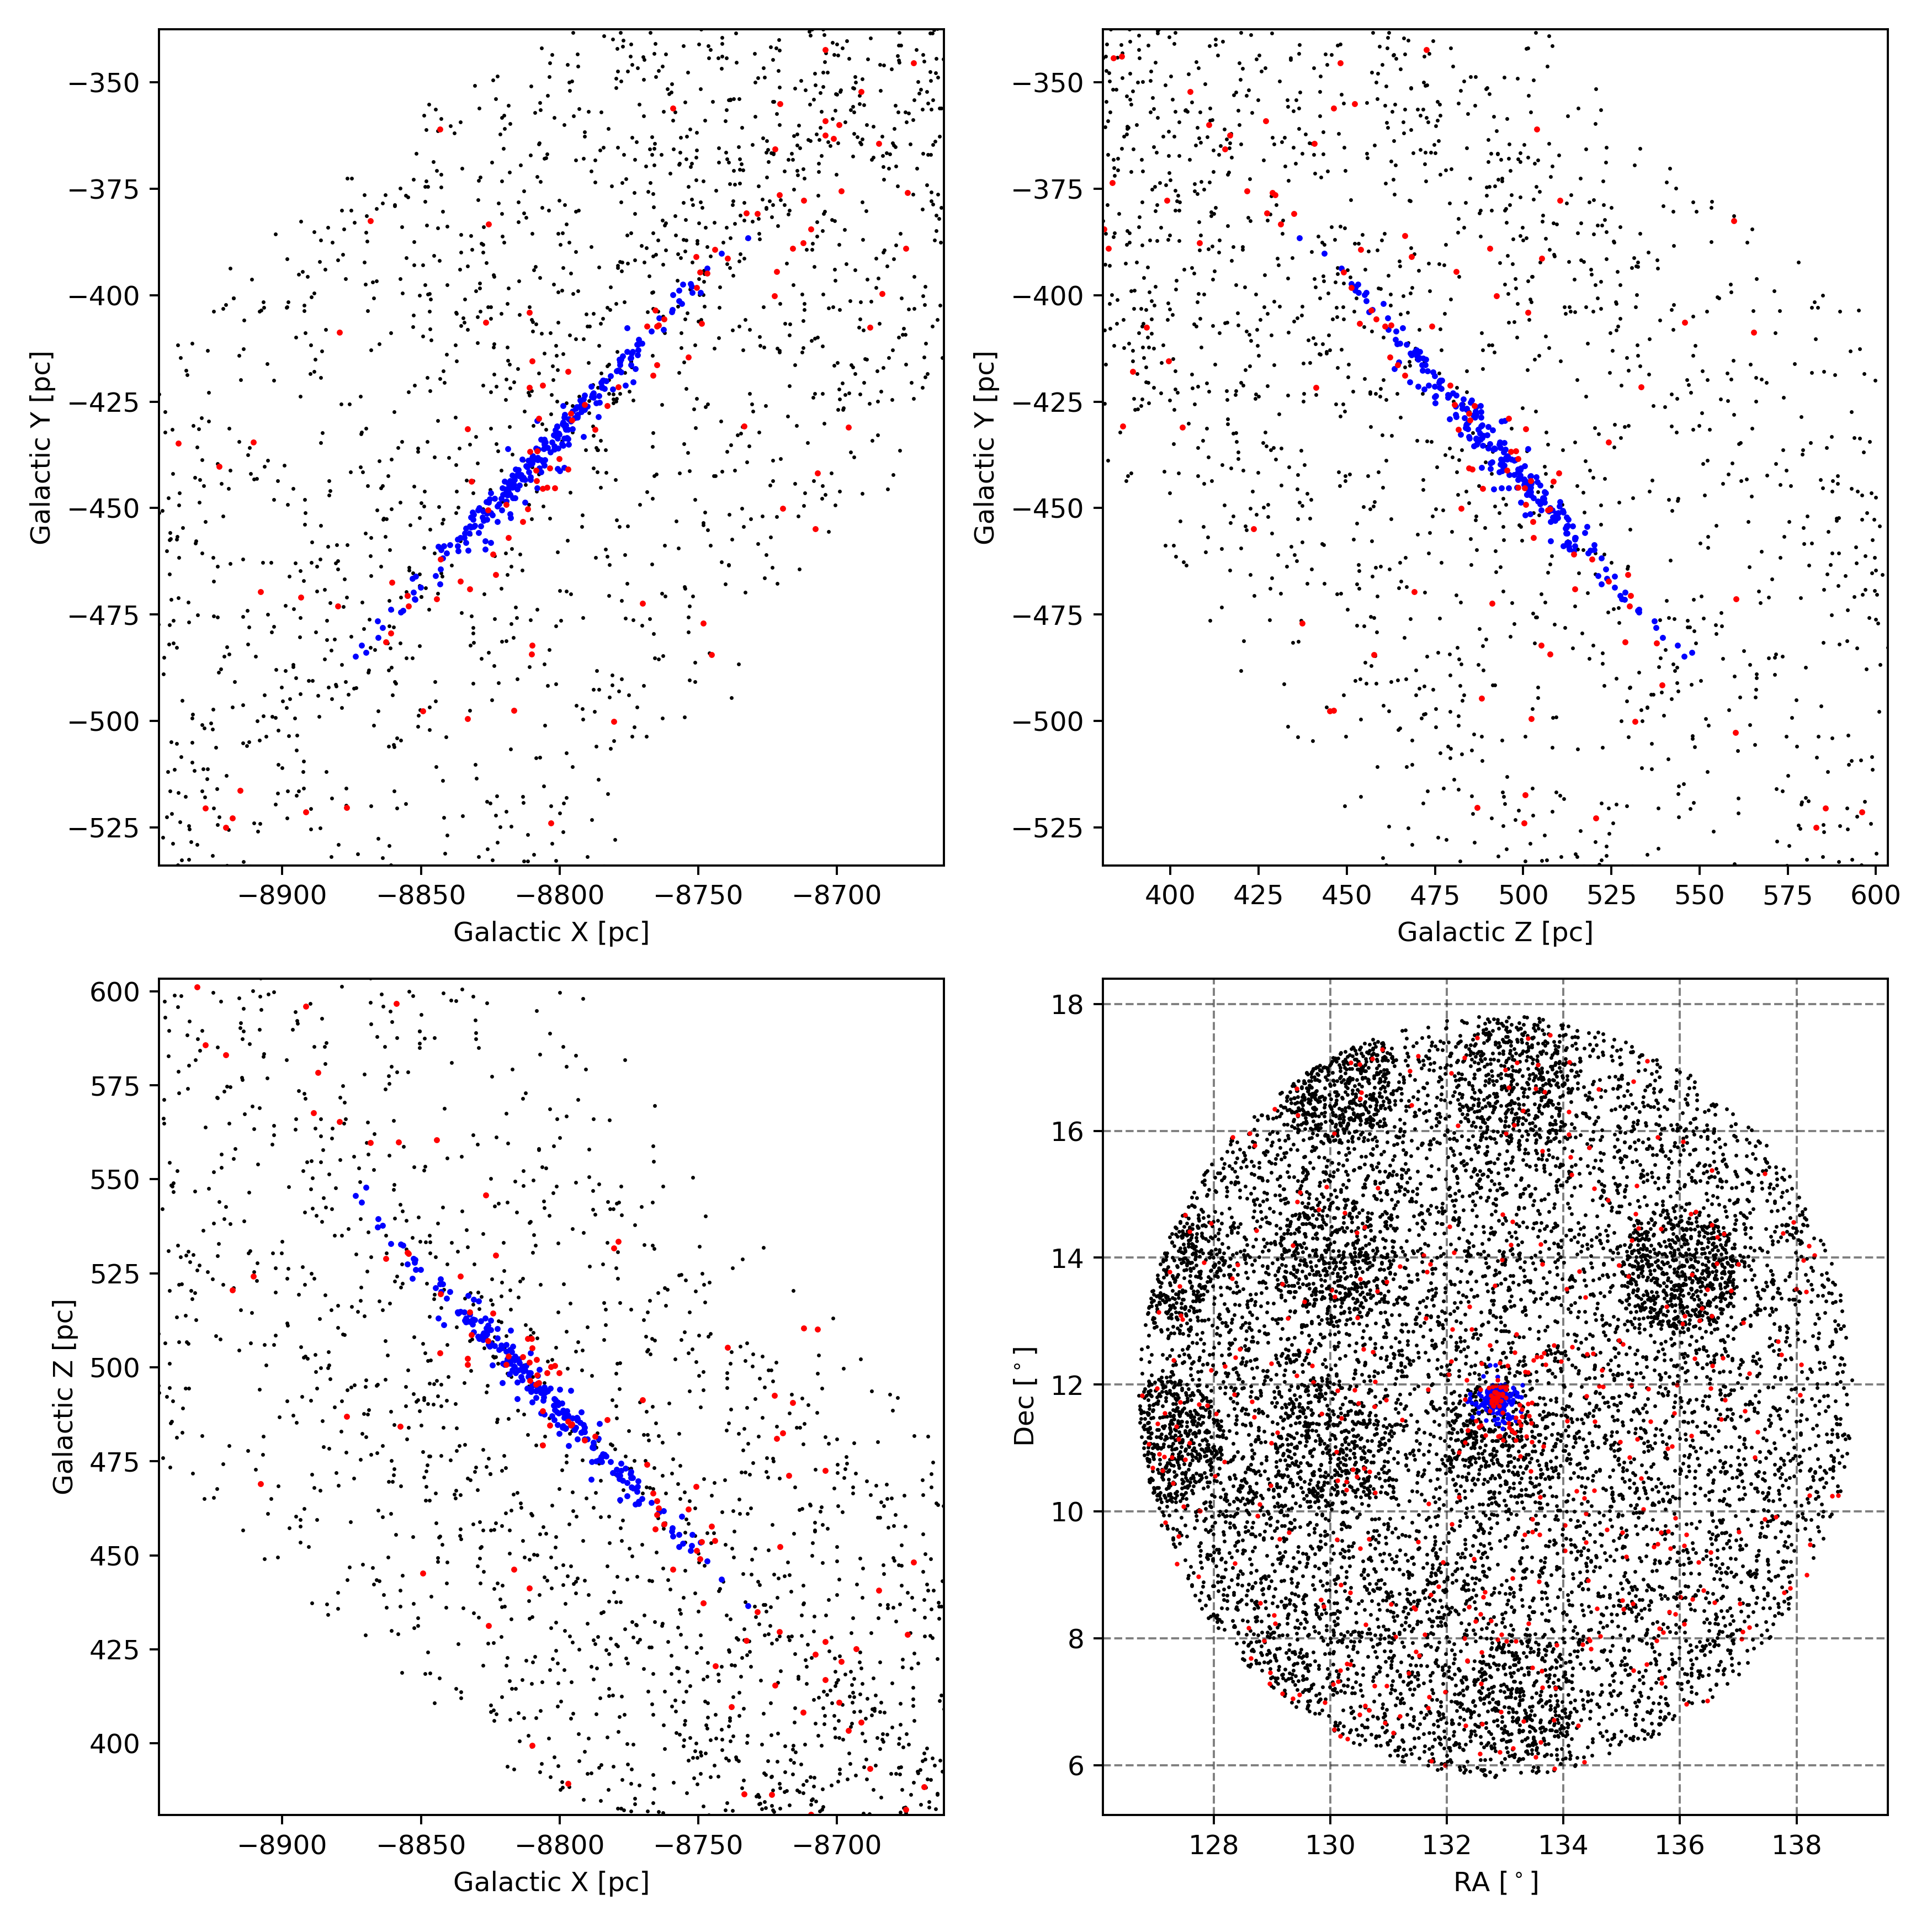
\includegraphics[width=\textwidth]{NGC_2682_possible_ejected-step1.png}
	\caption{Plots show the spatial distribution of the ejected candidates in red around the definite cluster members in blue. All other stars considered in the analysis are shown as black dots. First three panel shows the Galactic position of described cluster components. The denser circular patches of stars in the bottom right panel are not real stellar overdensities, but indicate regions where combined radial velocities of \G\ and \Gh\ are used. The example is given for the open cluster NGC 2682, which has the highest number of potentially ejected stars. Uncertainty of determined stellar distance is clearly evident as elongation of the main cluster body in the radial direction, away from the observers' position.}
	\label{fig:ejected_around_cluster}
\end{figure}

A much less energetic and more gradual mechanism that also influences the lifetime of an open cluster is tidal stripping of stars \cite{2006A&A...455L..17L}. It happens during clusters' journey through a more densely populated region such as galactic spiral arms. Tails reaching out of a cluster would, therefore, have elongated, probably slightly bent shape (not to be confused by the elongated cluster shape in Figure \ref{fig:ejected_around_cluster}), and not a spherical distribution as considered for ejection mechanism. In this section, we compare the chemical composition of known tidal structures (discovered in \Gs\ data by \citet{2019AA...627A...4R, 2019AA...627A.119C, 2019AA...621L...3M, 2019arXiv191206657Z}) of a few the \Gh\ open clusters with other previously defined and analysed structures. All of the aforementioned tidal structures were identified by different clustering methods of the same \G\ data and should, therefore, be in a sense similar to results of our orbital classification procedure. From the published tidal structures \cite{2019AA...627A...4R, 2019AA...627A.119C, 2019AA...621L...3M, 2019arXiv191206657Z}, we first removed all cluster members that were already identified by \citet{2018A&A...618A..93C} and consequently used in our procedure for the definition of clusters' chemical signature. In that way, our possibly ejected stars and tidal structures can be compared directly. Their overlap is shown in the fourth and fifth column of Table \ref{tab:cluster_stats_tails}. As the overlap between them is not zero, we can reliably say that we are all detecting similar kinematic structures using completely different approaches (but the same \G\ data). The identified structures therefore may or might not be related to neighbouring open cluster.

\begin{sidewaystable}
	\centering
	\caption{Statistics of detected stellar tidal structures around some of the clusters that were observed by the \Gh. The columns shown in the following order give information about: name of the analysed cluster, number of all stars found in the surrounding tidal structure, number of stars without cluster members, size of overlap between ejected and tail, number of unflagged \Gh\ observations among tidal structure, chemical similarity with parent open cluster, and reference source of the used data.}
	\begin{tabular}{l c c c c c r }
		\hline
		Cluster & Stars in & Without used & Common with & \Gh\ unflagged & Chemically & Membership\\
		& reference & cluster members & ejected & parameters (\% in & tagged & reference\\
		&  &  & (\% of ejected) & common with ejected) & (\% of valid) & \\
		\hline \hline
		Blanco 1   & 644 & 276 & 3 (50\%) & 7 (42.9\%) & 0 (0.0\%) & \citet{2019arXiv191206657Z} \\
		NGC 2632   & 1393 & 738 & 17 (22.1\%) & 25 (68\%) & 7 (28.0\%) & \citet{2019AA...627A...4R} \\
		NGC 2682   & 952 & 241 & 13 (14.4\%) & 18 (72.2\%) & 6 (33.3\%) & \citet{2019AA...627A.119C} \\
		Melotte 25 & 238 & 238 & 8 (30.8\%) & 57 (14.0\%) & 1 (1.8\%) & \citet{2019AA...621L...3M} \\
		\hline
	\end{tabular}
	\label{tab:cluster_stats_tails}
\end{sidewaystable}

Among randomly acquired The \Gh\ spectra, we observed some stars that where identified to belong to the kinematically discovered tidal structures around open clusters. If we consider only stars with unflagged the \Gh\ stellar parameters, the overlap between the sets is quite significant as more than 50\% of unflagged tail stars were also identified as possible ejected for every studied cluster. This significant overlap reduces probability of the tails having a completely different chemical signature than our selections, but at the same time confirms validity of our orbit tracing approach. 

For a tidal tail chemical tagging procedure, we used the same selection principle as previously described in Section \ref{sec:chem_ej_tag}. The results of the tagging experiment are presented in the last column of Table \ref{tab:cluster_stats_tails}. Majority of the tails have quite significant probability of being chemically similar to a nearby open cluster. 

\section{Summary and conclusions}
\label{sec:clusters_summary_conclusions}
Open clusters, as long known and widely studied stellar structures, still provide many opportunities for their exploration using new and improved information about their stellar components and neighbouring environment. In this chapter, we explored the latest multidimensional abundance data determined for stars observed in the scope of the \Gh\ survey, whose targets also consisted of stars in multiple open clusters. Combined with the \G\ kinematic information, a precise position, shape, and velocity of the cluster volume can be defined. We used the method of backward orbit integration to determine if any of the neighbouring stars could be kinematically traced back to the cluster and have the same chemical signature.

To verify that our orbital integration methodology gives sensible results, they were compared towards identified cluster tidal structures around the same open clusters. Given non zero overlap in all cases, we are confident that our structures are also related to the main cluster body.

Deepened analysis of field and cluster abundance patterns showed improvement in the quality of determined abundances (in comparison towards older \Gh\ releases), but at the same time revealed the pitfalls of blindly using massively determined abundances for blind chemical tagging experiments that are highly desired in the community of galactic archaeology. Identified problems can successfully be overcome by applying differential analysis, which in our case showed some encouraging success of using the \Gh\ abundance data as tracers of stellar birth signatures of individual stars. The tagging experiment showed that it was more likely that we could chemically tag a kinematically pre-selected star than a random nearby star. For a much firmer confirmation, we would require more observations as some of the cluster components were sparsely observed by the \Gh.

The explored methodology depends on the quality and correctness of the determined abundance trends. From the current data, it seems that identified abundance trends are valid only for an individual cluster as they can vary among them. This decreases possibility of preforming differential chemical tagging on larger, potentially galactic, scales.

To improve the parameters used in this chapter, we would have to analyse cluster members as a homogeneous structure that was formed at the same time. This adoption of formation time would force the use of a single isochrone and stellar age for all members, improving their determined \Logg, \Feh, and consequently also stellar surface chemical composition. Our first experiments with the mentioned analysis upgrade already show significant improvements in the stability of the trends and reduction of abundance scatter among cluster members.

\chapter{Chemically peculiar stars}
\label{chap:peculiars_chem}
This chapter has been adapted from the published paper titled \textit{The GALAH survey: a catalogue of carbon-enhanced stars and CEMP candidates} \cite{2019MNRAS.483.3196C} that was prepared and written by the author of this Doctoral thesis. The used computer code was published on GitHub platform  \footnote{\url{https://github.com/kcotar/GALAH-survey-Carbon-enhanced-stars}} and results of the analysis as a catalogue on VizieR service  \footnote{\url{http://vizier.u-strasbg.fr/viz-bin/VizieR?-source=J/MNRAS/483/3196}}.

In the previous chapter, we saw that the chemical tagging of open cluster stars is far from a straightforward process in large spectroscopic studies and relies on many assumptions. One of them is that analysed spectra are of normal, non-active stars whose outer layer was not polluted by other stars or anyhow modified during their lifetime. To improve the accuracy of chemical tagging, such peculiarities in acquired spectra must be detected and derived parameters effectively filtered out before any analysis is performed. One of such peculiarities are stellar chemical enrichments that are usually results of pollution by nearby evolved stars, such as novae and supernovae. This chapter deals with the identification of carbon-enhanced stars using supervised and unsupervised classification algorithms. The chapter begins with a brief introduction of carbon-enhanced stars, and their historical and present importance in Section \ref{sec:intro_cemp}, which is followed by the description of the used algorithms for the detection of carbon-enhanced stars in Section \ref{sec:classification_cemp}. Properties of the classified objects are investigated in Section \ref{sec:analysis_cemp}, CEMP candidates are a focus of Section \ref{sec:cemp_cemp}, with Section \ref{sec:asiago_cemp} describing a follow-up study for one of them. Final remarks are given in Section \ref{sec:summary_cemp}.

\section{Introduction}
\label{sec:intro_cemp}
Chemically peculiar stars whose spectra are dominated by carbon molecular bands were first identified by \citet{1869AN.....73..129S}. Their spectra are characterised by enhanced carbon absorption bands of CH, CN, SiC$_2$, and C$_{2}$ molecules, also known as Swan bands. Possible sources of enhancement are dredge-up events in evolved stars \cite{1983ApJ...275L..65I}, enrichment by carbon-rich stellar winds from a pulsating asymptotic giant branch (AGB) star, which settles on a main sequence companion \cite{1995MNRAS.277.1443H}, or it can be the result of a primordial enrichment \cite{2016ApJ...833...20Y}. Historically, high latitude carbon stars, presumed to be giants, were used as probes to measure the Galactic rotation curve \cite{2013Ap.....56...68B}, velocity dispersion in the Galactic halo \cite{1991AJ....101.2220B}, and to trace the gravitational potential of the Galaxy.  

Because of their strong spectral features, the most prominent candidates can easily be identified from large photometric surveys \cite{2002AJ....124.1651M, 2004AJ....127.2838D}. Specific photometric systems \cite{1960MNRAS.120..287G, 1968AJ.....73..313M, 1970A&AS....1..199H} were defined in the past to discover and further classify stars with enhanced carbon features in their spectra. Specifics of those systems were catalogued, compared, and homogenised by \citet{2000A&AS..147..361M} and \citet{2003A&A...401..781F}.

Other useful data come from low-resolution spectroscopic surveys, whose classification identified from a few hundred to a few thousand of those objects \cite{2001A&A...375..366C, 2013ApJ...765...12G, 2013AJ....146..132L, 2016ApJS..226....1J, 2018ApJS..234...31L}. High-resolution spectroscopy is required to search for candidates with less pronounced molecular absorption features or to determine their stellar chemical composition. Multiple studies have been carried out to determine accurate abundances of metal-poor stars \cite{1997ApJ...488..350N, 2002ApJ...567.1166A, 2004A&A...416.1117C, 2005ESASP.560..433B, 2006AJ....132..137C, 2007ApJ...655..492A, 2007ApJ...670..774N, 2011ApJ...742...54H, 2013ApJ...762...26Y, 2014AJ....147..136R, 2015ApJ...807..173H, 2015ApJ...807..171J}. Such detailed abundance information is especially important for the analysis and classification of chemically peculiar objects \cite{2013ApJ...778...56C}.

Today, the most sought after, of all carbon-enhanced stars, are the carbon-enhanced metal-poor (CEMP) ones whose fraction, among metal-poor stars, increases with decreasing metallicity \Meh\ \cite{1992AJ....103.1987B, 1997ApJ...488..350N, 1999ASPC..165..264R, 2005ApJ...633L.109C, 2005ApJ...625..825L, 2005AJ....130.2804R, 2006ApJ...652.1585F, 2007PhDT........22M, 2012ApJ...744..195C, 2013AJ....146..132L, 2013ApJ...762...27Y,  2014ApJ...797...21P, 2018ApJ...861..146Y}. Amongst these, those near the main-sequence turn-off are expected to be of particular importance, as they may have accreted enough material from their AGB companion to produce an observable change in their atmospheric chemical composition \cite{2004ApJ...611..476S, 2014MNRAS.441.1217S, 2015ApJ...807..173H}. The accreted material could provide insight into the production efficiency of neutron capture elements in AGB stars \cite{2007ApJ...655..492A}. Multiple studies show that a peculiar observed abundance pattern and carbon enrichment in a certain type of CEMP stars could be explained by the supernova explosions of first-generation stars that enriched the interstellar medium \cite{2003Natur.422..871U, 2005ApJ...619..427U, 2014ApJ...785...98T, 2018MNRAS.tmp.2127B}. The exact origin and underlying physical processes governing multiple classes of CEMP stars are not yet fully understood and are a topic of ongoing research \cite{2014ApJ...788..180C, 2016ApJ...833...20Y, 2018MNRAS.475.4781C}. Classification into multiple sub-classes is performed using the abundance information of neutron-capture elements \cite{2005ARA&A..43..531B, 2013A&A...552A.107S, 2015ApJ...814..121H, 2016ApJ...833...20Y} that are thought to originate from different astrophysical phenomena responsible for the synthesis of those elements.

\section{Detection procedure}
\label{sec:classification_cemp}
To search for carbon-enhanced stars in the GALAH data set, we focused on spectral features that can be distinguished and are known markers of carbon enhancement. Instead of using one very weak atomic carbon absorption line (at 6587.61~\AA), used by \TC\ to determine \Cfe\ abundance, we focused on a region between 4718 and 4760~\AA\ observed in the blue arm that covers 4718--4903~\AA\ in its rest-frame. In this range we can, depending on the radial velocity of the star, observe at least four Swan band features \cite{1927RSPTA.226..157J} with their band heads located at approximately 4715, 4722, 4737, and 4745~\AA. The bands are caused by molecules that contain carbon. Therefore their shape is not a simple single absorption line, but a wedge-like absorption feature - a sequence of molecular vibrational bands. Historically, the bands have also widely been used for the exploration of cometary spectra.

Carbon enhancement is observable in spectra as a strong additional absorption feature (Figure \ref{fig:carbon_example}) that is the strongest at the wavelength of the band's head. After that its power gradually decreases with decreasing wavelength. The most prominent and accessible for all of the spectra is a feature located at 4737~\AA, produced by a $^{12}$C$^{12}$C molecule. If other carbon features, like the one produced by a $^{13}$C$^{12}$C molecule at 4745~\AA\ (shown in Figure \ref{fig:carbon_example2}) are present in the spectrum, the carbon isotope ratio $^{12}$C/$^{13}$C in a star can be determined. Its determination was not attempted in the scope of this chapter.

\begin{figure}
	\centering
	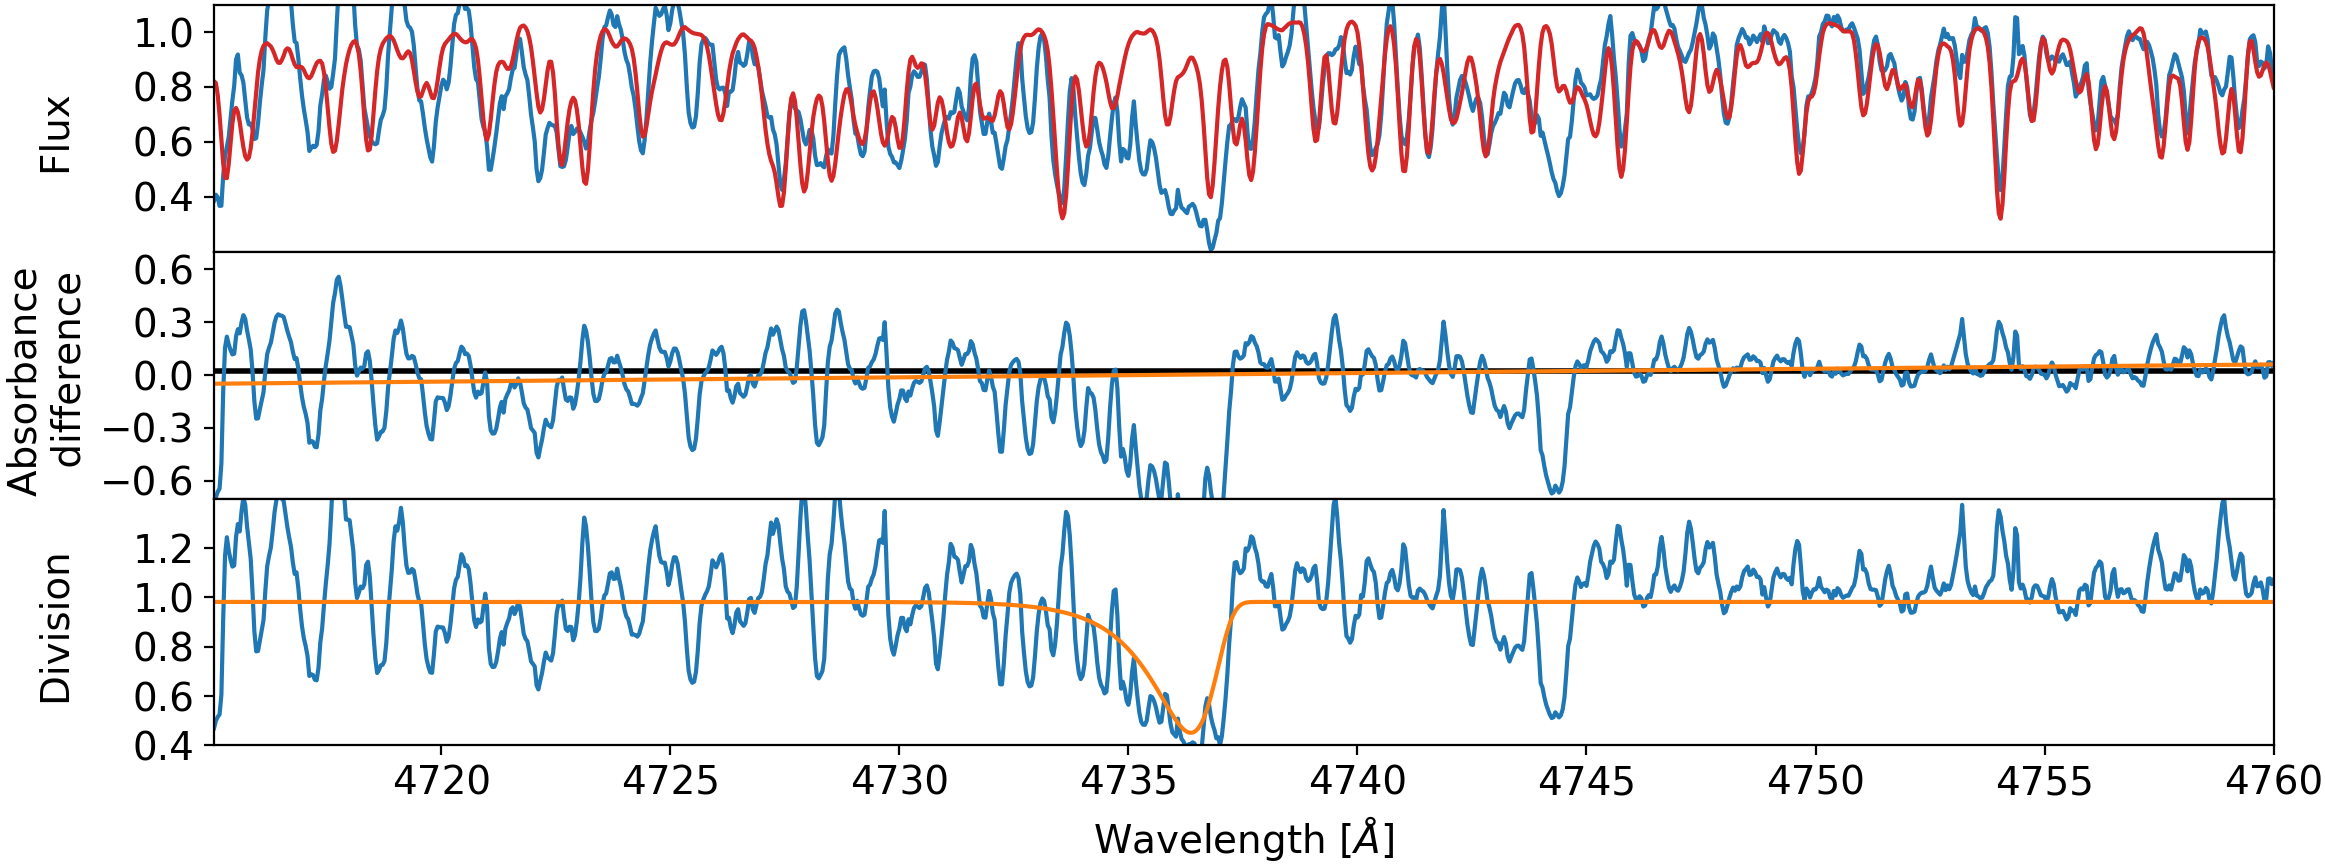
\includegraphics[width=\textwidth]{rich_160515003401143.png}
	\caption{Equivalent plot as in the Figure \ref{fig:carbon_example} but presenting an example of a metal-rich star with multiple strong Swan features around 4737 and 4745 \AA. Presented star has a 2MASS identifier J13121354-3533120 and is known Galactic carbon star \cite{2001BaltA..10....1A}.}
	\label{fig:carbon_example2}
\end{figure}

Detection of spectral features was tackled using two different classification procedures. First, a supervised procedure was used to identify the most prominent spectra with carbon enhancement. The supervised selection was based on the following two assumptions: knowledge about where in the spectrum those features are located and how they look. This assumption was augmented with an unsupervised dimensionality reduction algorithm that had no prior knowledge about the desired outcome. The goal of a dimensionality reduction was to transform n-dimensional spectra onto a 2D plane where differences between them are easier to analyse. The unsupervised algorithm was able to discern the majority of carbon-enhanced spectra from the rest of the data set and enabled us to discover spectra with less prominent carbon enhancement features.

\begin{figure}
	\centering
	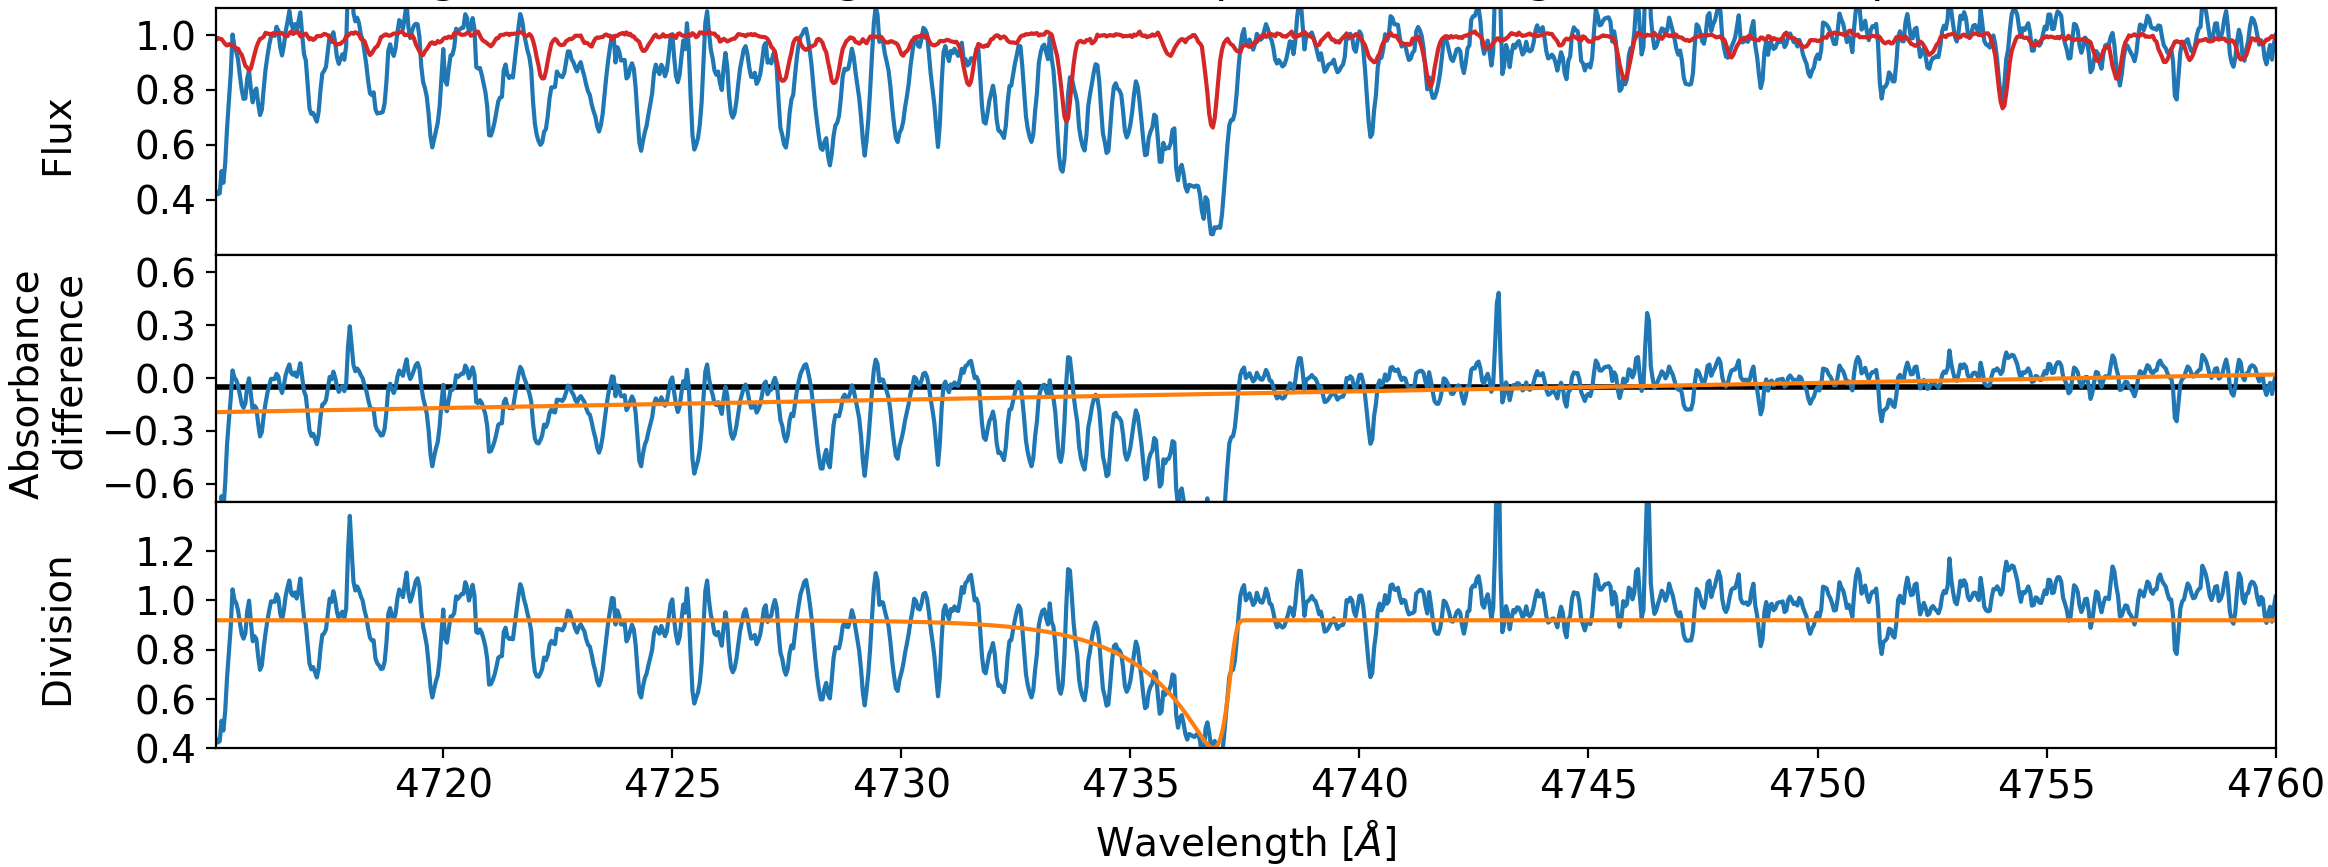
\includegraphics[width=\textwidth]{cemp_cand_150412003601009.png}
	\caption{Example of a metal-poor carbon-enhanced candidate with strong Swan absorption feature at 4737~\AA, caused by the carbon C$_2$ molecules. The first panel shows the stellar spectrum in blue and a corresponding reference median spectrum in red. The reference median spectrum was computed as the per-pixel median flux value of spectra with similar stellar parameters (selection defined in Section \ref{sec:supervised}) as the spectrum shown in blue. The spectral difference (second panel) and division (third panel) were computed from those two spectra. The middle panel shows in orange a linear fit to the spectral difference that was used to identify spectra with the reduction problems on the blue border of the spectral range. The black horizontal line gives the median value of the spectral difference. The orange curve in the last panel shows a fit that was used to determine the strength of the observed carbon feature. The shown spectrum belongs to a star with a Two Micron All-Sky Survey (2MASS, \cite{2006AJ....131.1163S}) identifier J11494247+0051023 and iron abundance \Feh\ of $-1.17$, as determined by \TC.}
	\label{fig:carbon_example}
\end{figure}

\subsection{Supervised classification}
\label{sec:supervised}
To search for additional absorption features that are usually not found in spectra of chemically normal stars, we first built a spectral library of median spectra based on an initial rough estimate of stellar physical parameters that are derived by the automatic reduction pipeline, described in detail by \citet{2017MNRAS.464.1259K}. The median spectrum for every observed spectrum in our data set was computed from physically similar spectra. Their effective temperature \Teff\ had to be in the range of $\Delta$\Teff~=~$\pm75$~K, surface gravity \Logg\ in the range of $\Delta$\Logg~=~$\pm0.125$~dex, and iron abundance \Feh\ in the range of $\Delta$\Feh~=~$\pm0.05$~dex around the stellar parameters of the investigated spectrum. The median spectrum was calculated only for observed targets with at least five similar spectra in the defined parameter range and with minimal noise level of SNR~=~$15$ per resolution element, as determined for the blue spectral arm. All considered spectra were resampled to a common wavelength grid with 0.04~\AA\ wide bins and then medianly combined. The automatic reduction pipeline \cite{2017MNRAS.464.1259K} performed the normalisation of the spectra along with the radial velocity determination and the corresponding shift to the rest frame. We checked that spectral normalisation and radial velocity determination are adequate also for carbon-enhanced stars. The normalisation procedure was done using a polynomial of low-order that is not strongly affected by the Swan band features or similar spectral structures. The radial velocity of a star was determined as an average of radial velocities that were independently determined for the blue, green, and red spectral arm. If one of the arms has a radial velocity deviating for more than two times the difference between the other two, it was excluded from the average (further details in \citet{2017MNRAS.464.1259K}). Therefore the final velocity should be correct even if one of those arms contains features that are not found in the set of reference spectra used in the cross-correlation procedure.

With the limitation of at least five spectra used for the computation of the median spectrum, some possibly carbon-enhanced stars could be excluded from the supervised classification. The final number of spectra analysed by this method was 558,053.

Spectra, for which we were able to determine the median spectrum of physically similar objects, were analysed further. In the next step, we tried to determine possible carbon enhancement by calculating a flux difference and flux division between the observed stellar and median spectra, as shown in Figure \ref{fig:carbon_example}.

In order to describe the position, shape, and amplitude of the Swan feature with its head at 4737~\AA, we fitted a function that is based on a Log Gamma ($\log{}\Gamma$) distribution. The distribution, with three free parameters, was fitted to the division curve, where the Swan feature is most pronounced. Division curve, shown in the bottom panel of Figure \ref{fig:carbon_example}, was computed by dividing the observed spectrum with its corresponding median spectrum. The fitted function $f$ can be written as:
\begin{equation}
\centering
f(\lambda) = f_0 - \log{}\Gamma(\lambda, S, \lambda_0, A).
\label{equ:loggamma}
\end{equation}
The shape of the curve is defined by an offset $f_0$, shape parameter $S$, centre wavelength $\lambda_0$, and amplitude $A$ of $\log{}\Gamma$ distribution, where $\lambda$ represents rest wavelengths of the observed spectrum. This function was selected because of its sharp rise followed by the gradual descent that matches well with the shape of a residual absorption observed in the Swan regions. The steepness of the rising part is determined by the parameter $S$ (lower value indicates steeper raise) and its vertical scaling by the parameter $A$. We are not aware of any other profile shapes used for fitting Swan bands in the literature.

To narrow down possible solutions for the best fitting curve, we used the following priors and limits. The initial value for the parameter $f_0$ was set to a median of all pixel values in the division curve and allowed to vary between $0.5$ and $1.5$. The limiting values are, however, newer reached. The centre of the $\log{}\Gamma$ distribution $\lambda_0$ was set to $4737$~\AA\ and was allowed to vary by $2$~\AA. Wavelength limits were set to minimise the number of misfitted solutions, where the best fit would describe the nearby spectral absorption lines not present in the median spectra or problematic spectral feature caused by the spectral data reduction as shown by Figure \ref{fig:bad_fit1}. We did not set any limits on parameters $A$ and $S$ in order to catch fitted solutions describing a spectrum difference that is different from the expected shape of the molecular absorption band.

By integrating the surface between the offset $f_0$ and the fitted curve we calculated the strength of the Swan band. The integral (\texttt{swan\_integ} in Table \ref{tab:out_table}) is derived between 4730 and 4738~\AA. It should not be used as a substitute for a carbon abundance measurement, but only to sort the detections of carbon-enhanced stars by their perceivable strength of the Swan band.

\begin{figure}
	\centering
	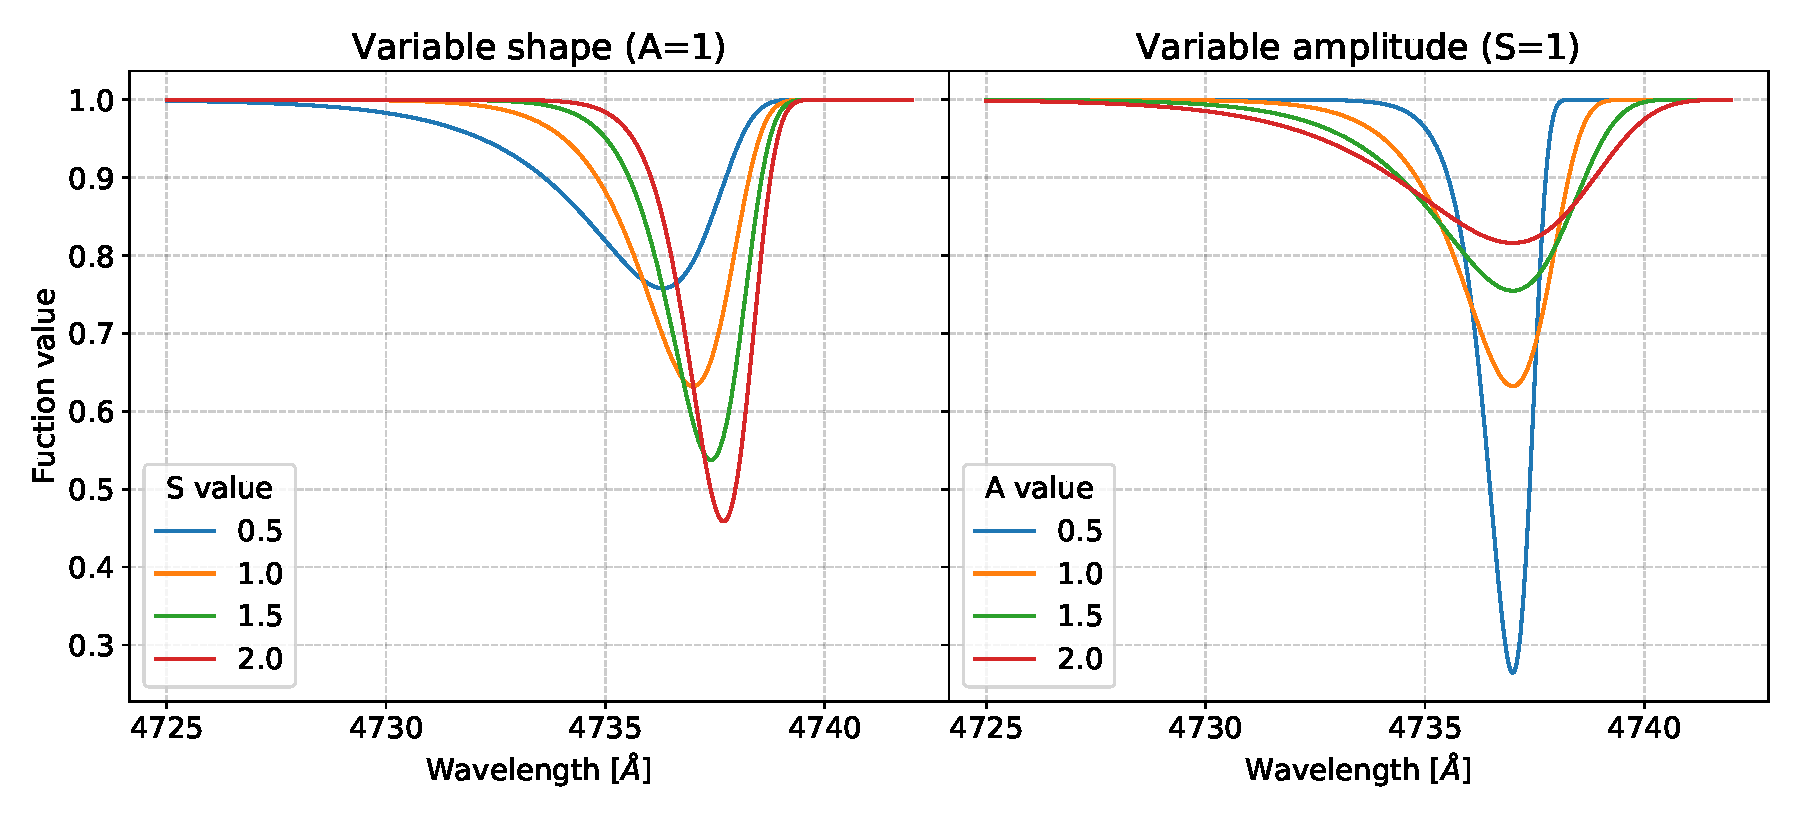
\includegraphics[width=0.95\textwidth]{variable_A_S.pdf}
	\caption{Visualization of selecting appropriate values of shape and amplitude parameters during the function fitting explained in Section \ref{sec:supervised}. The left panel shows effect of varying shape parameter $S$ and the right panel varying amplitude parameter $A$ in Equation \ref{equ:loggamma}.}
	\label{fig:varibles_loggamma}
\end{figure}

\begin{table}
	\centering
	\caption{List and description of the fields in the published catalogue of detected objects and objects matched with multiple literature sources.}
	\label{tab:out_table}
	\begin{tabular}{l c l}
		\hline
		Field & Unit & Description \\ 
		\hline
		\texttt{source\_id} & & {\it Gaia} DR2 source identifier \\
		\texttt{sobject\_id} & & Unique internal per-observation star ID \\
		\texttt{ra} & deg & Right ascension from 2MASS, J2000 \\
		\texttt{dec} & deg & Declination from 2MASS, J2000 \\
		\texttt{det\_sup} & bool & Detected by the supervised fitting method \\
		\texttt{det\_usup} & bool & Detected by the t-SNE method \\
		\texttt{swan\_integ} & \AA & Swan band strength if determined \\
		\texttt{teff} & K & \TC\ effective temperature \Teff \\
		\texttt{e\_teff} & K & Uncertainty of determined \Teff \\
		\texttt{logg} & $\log$(cm/s$^{2}$) & \TC\ surface gravity \Logg \\
		\texttt{e\_logg} & $\log$(cm/s$^{2}$) & Uncertainty of determined \Logg \\
		\texttt{feh} & dex & \TC\ iron abundance \Feh \\
		\texttt{e\_feh} & dex & Uncertainty of determined \Feh \\
		\texttt{flag\_cannon} & int & \TC\ flags in a bit mask format \\
		\texttt{type} & & G for giants and D for dwarfs \\
		\texttt{rv\_var} & bool & Is radial velocity variable. \\
		 & & Minimal radial velocity change of $0.5$~\kms \\
		\texttt{li\_strong} & bool & Shows strong lithium absorption \\
		 & & \TC\ \Life\ had to be >~$1.0$ \\
		\texttt{cemp\_cand} & bool & Is star CEMP candidate \\
		 & & \TC\ \Feh\ had to be >~$-1.0$ \\
		\texttt{bib\_code} &  & ADS bibcode of the matched literature source \\
		\hline
	\end{tabular}
\end{table}

With so many spectra in our data set, unexpected reduction and analysis problems can hinder the selection of carbon-enhanced stars. In the first iteration, the results were ordered only by the value of the integrated Swan band region, but this proved to select too many spectra with reduction problems. Most of the problematic detections were caused by the incorrect normalisation of spectra with strong, non-carbon molecular bands. This normalisation issue is best observable at the border of a spectral range, where Swan bands are located in the case of HERMES spectra. There, normalisation can be poorly defined in the case of numerous nearby absorption lines. In order to prevent miss-detections, additional limits on the shape ($S <= 1$) and amplitude ($A <= 1$) of the $\log{}\Gamma$ distribution were used to filter out faulty fitting solutions. Impact of varying $A$ and $S$ on the shape of the function is shown in Figure \ref{fig:varibles_loggamma}. Selecting too large parameter $S$ causes function to be too narrow as shown in Figure \ref{fig:bad_fit1}. Similarly, too large amplitude $A$ results in function with reduced skewness as fitted to the spectrum in Figure \ref{fig:bad_fit2}. 

Figure \ref{fig:bad_fit2} represents misfitted example where the function $f(\lambda)$ was fitted to the absorption lines of a double-lined spectroscopic binary, producing a shape of the function that is not characteristic for the analysed molecular band head. To remove spectra with reduction problems or peculiarity that would result in wrongly determined strength of the Swan band, we are also analysing the slope of the spectral difference and its integration in the limits of the Swan bands. One of the spectral trends that we are trying to catch with those indicators is shown in Figure \ref{fig:bad_fit2}, where spectral difference and its linear fit are steeply rising at the border of the spectrum.

By visual inspection of the algorithm, diagnostic plots are shown in Figure \ref{fig:carbon_example}, we limited a final selection to 400 spectra with the strongest carbon enhancement that was still visually recognisable. The last selected spectrum is shown in the Figure \ref{fig:carbon_last_supervised}. Selection of spectra with lower enhancement would introduce possibly wrong classification of stars whose enhancement is driven by spectral noise levels, data reduction or any other process that has a subtle effect on the spectral shape.

\subsection{Unsupervised classification}
\label{sec:unsupervised}
With numerous spectra of different stellar types, chemical composition, and degree of carbon enhancement, some of them might show different carbon features or be insufficiently distinctive to be picked out by the above described supervised algorithm.

Another analysis technique, which is becoming increasingly popular is a dimensionality reduction procedure named t-distributed Stochastic Neighbor Embedding (t-SNE, \cite{van2008visualizing}) that has already proved to be beneficial in comparison and sorting of unknown spectral features of the same data set \cite{2017ApJS..228...24T}. With the method, we aim to reduce the number of dimensions while preserving the structure of analysed data. In our case of a stellar spectrum, we have numerous dimensions (one per wavelength bin), among which we want to look for groups of data points. This search for groups could be done in the original space with many dimension, but visualisation of such dataset is problematic. As the relations between wavelength bins are not linear, methodologies such as Principal Component Analysis (PCA), have to be supplemented with non-linear methodologies; t-SNE for example. An additional problem, we are dealing with is a density of investigated spectra. As peculiar spectra are usually in the minority, the algorithm must recover global and local structures. t-SNE is able to map data sets with high variations in density, so it is able to resolve small, local details, as well as the global picture. This feature is achieved by the internal use of a Student's distribution. The algorithm is fine-tuned using the property perplexity that controls whether t-SNE is more sensitive to global or local structures. This property is comparable to setting the number of nearest neighbours taken into consideration. The role of the perplexity can be tested in an online interactive tool produced by \citet{wattenberg2016how}. After computing similarities between all pairs of the investigated spectra, the algorithm tries to find the best transformation that optimally arranges spectra in a 2D plane. As the transformation is variable and non-linear, the actual distance between two objects in a final 2D plane does not linearly depend on the spectral similarity measure. This property of the t-SNE algorithm additionally ensures more homogeneous coverage of the 2D plane in comparison to other dimensionality reduction methods.

\begin{figure}
	\centering
	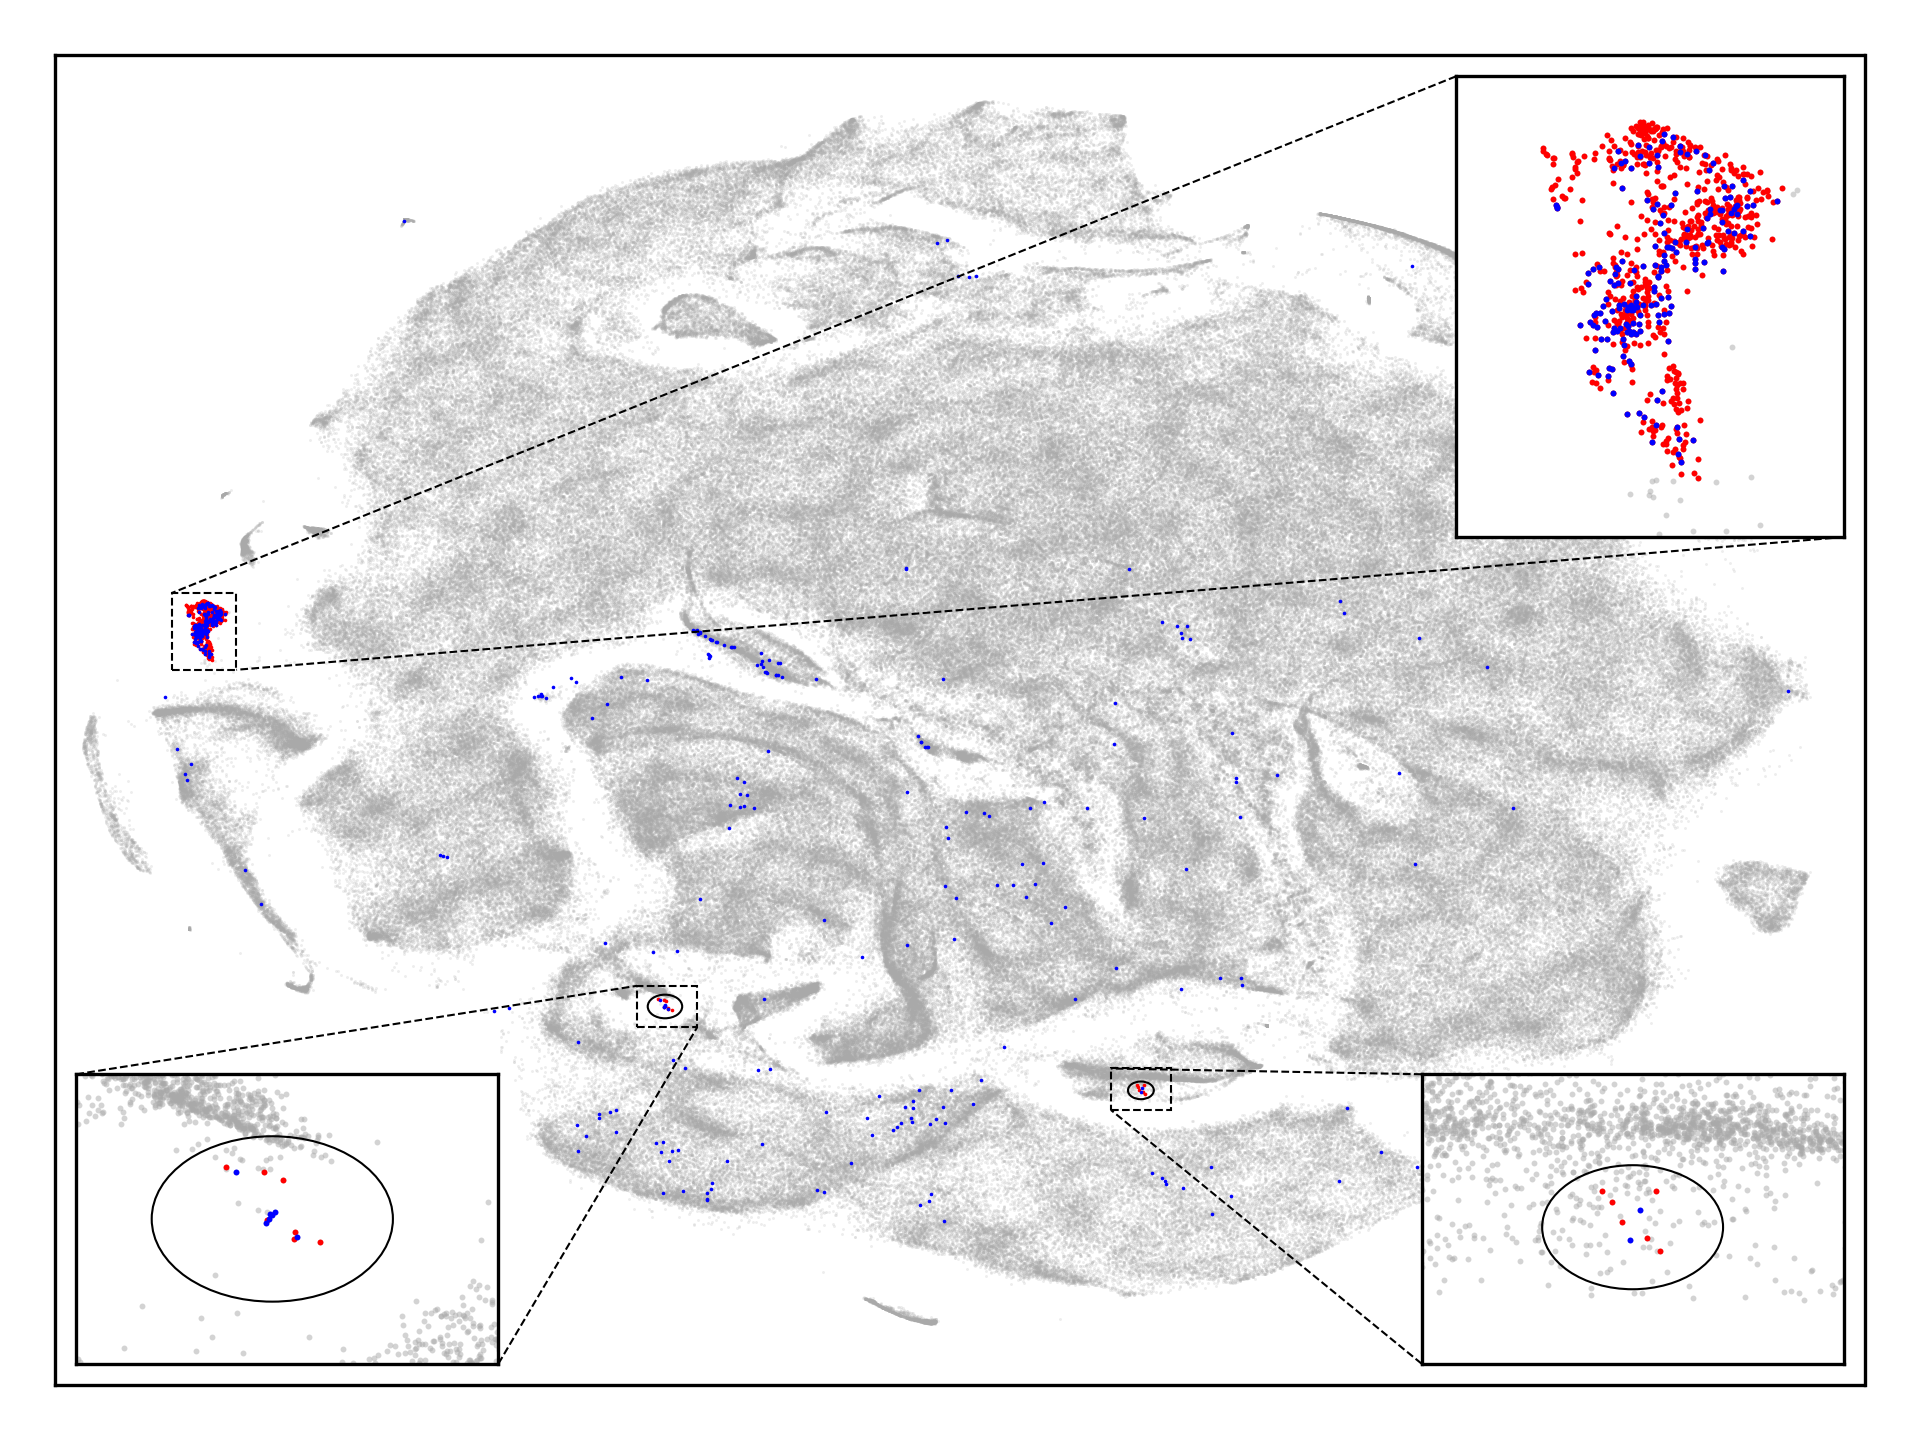
\includegraphics[width=\textwidth]{tsne_circles.png}
	\caption{t-SNE projection of 588,681 observed spectra ranging between 4720 and 4890~\AA. Red dots (756 spectra) mark a clump in the projection that was manually selected to contain carbon-enhanced spectra. Superimposed blue dots represent carbon-enhanced spectra determined by the supervised algorithm. Outside the t-SNE selected clump, we have 224 spectra that were determined to be carbon-enhanced only by the supervised method. All other analysed spectra are shown in grey shades, depending on their density in the 2D projection. Two ellipses indicate regions where the majority of CEMP candidates is located in the projection.}
	\label{fig:tsne_plot}
\end{figure}

The t-SNE projection shown in Figure \ref{fig:tsne_plot} was computed from normalised spectra between 4720 and 4890~\AA. To maximise the number of analysed spectra, no other limiting cuts than the validity of the wavelength solution (bit 1 in \texttt{red\_flag} set to 0 by reduction pipeline \cite{2017MNRAS.464.1259K}) in this arm was used. This resulted in 588,681 individual spectra being analysed by the automatic unsupervised algorithm. This is $\sim30$k more spectra than in the case of supervised classification, where we applied more strict criteria for the selection of analysed spectra (Section \ref{sec:supervised}). 

Without any prior knowledge about the location of objects of interest in the obtained projection, we would have to visually analyse every significant clump of stars in order to discover whether the carbon-enhanced population is located in one of them. This can be simplified by adding the results of the supervised classification into this new projection. In Figure \ref{fig:tsne_plot}, the stars identified by the supervised classification are shown as blue dots plotted over grey dots representing all spectra that went into the analysis. The majority of blue dots are located in a clump on the left side of the projection. A high concentration of objects detected by a supervised method leads us to believe that this isolated clump represents carbon-enhanced objects in the t-SNE projection. To select stars inside the clump, we manually have drawn a polygon around it.

Inspection of other blue labelled spectra outside the main clump revealed that their slight carbon enhancement could not be identified by the t-SNE similarity metric as another spectral feature might have dominated the spectral comparison.

\begin{figure}
	\centering
	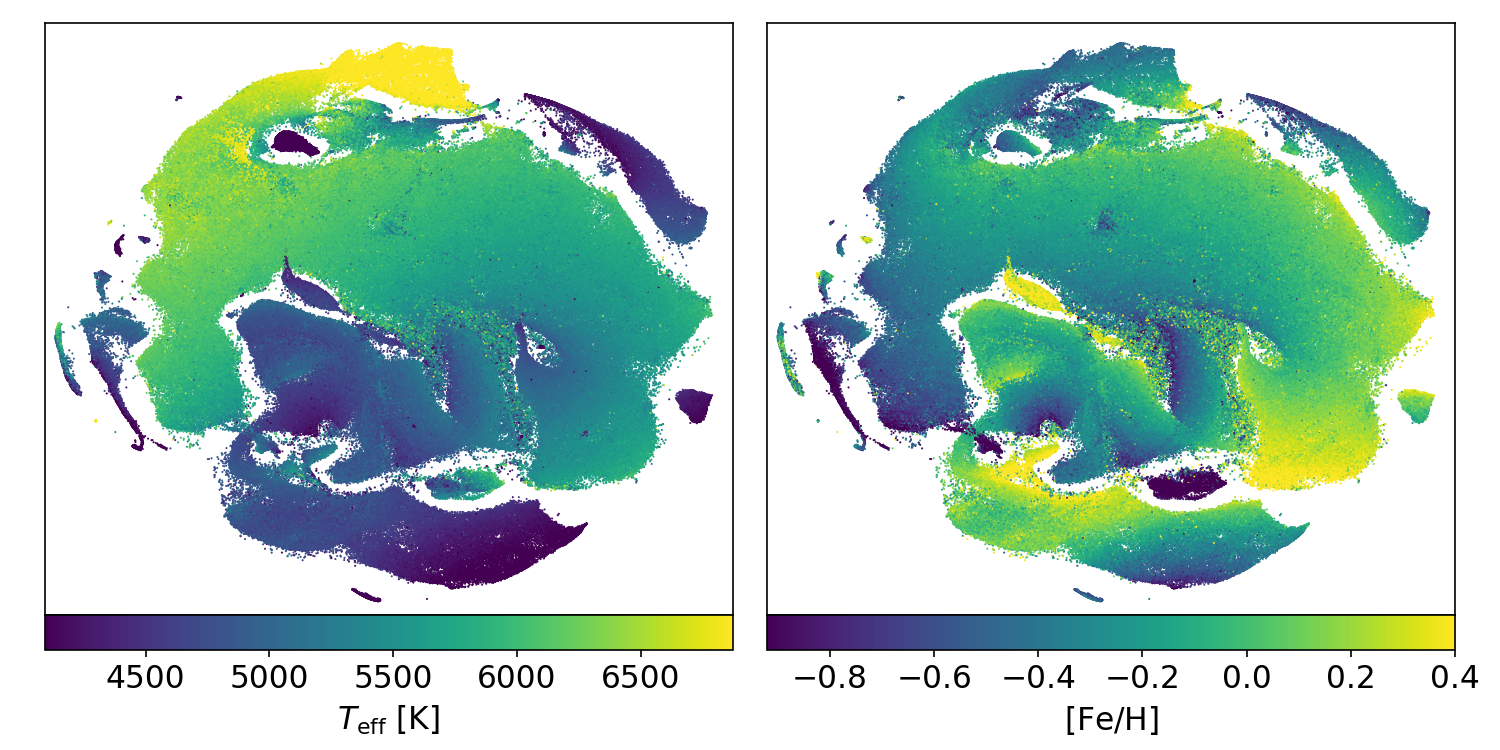
\includegraphics[width=\textwidth]{tsne_params_notitle.png}
	\caption{Spatial distribution of all available measurements of \Teff\ (left panel) and \Feh\ (right panel) as determined by \TC. Dots, representing analysed spectra in the t-SNE projection, are colour coded by their parameter values. Colours and their corresponding values are explained by a colourbar under the graph.}
	\label{fig:tsne_teff_feh}
\end{figure}

Additional exploration of the t-SNE projection revealed two smaller groups of metal-poor carbon-enhanced spectra located inside ellipses shown in Figure \ref{fig:tsne_plot}. A confirmation that those regions are populated with metal-poor stars can be found in Figure \ref{fig:tsne_teff_feh} where the dots representing spectra in the projection are colour coded by \Feh\ and \Teff. To maximise the number of those objects in the published catalogue, we manually checked all undetected spectra in the vicinity of the detected ones. This produced an additional 13 CEMP detections.

\subsubsection{t-SNE limitations}
\begin{figure}
	\centering
	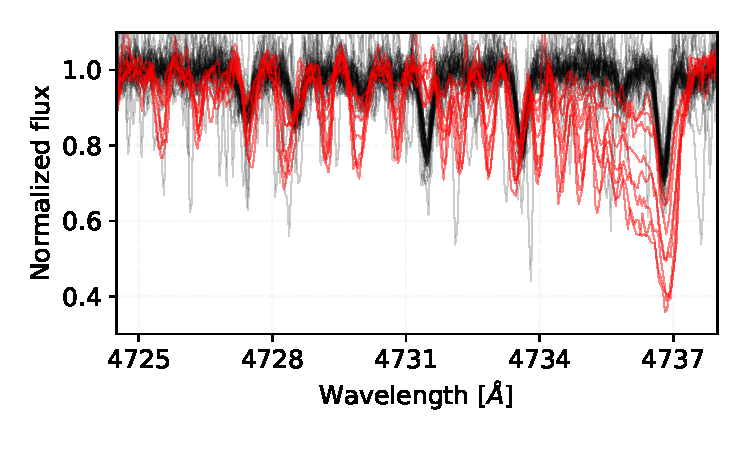
\includegraphics[width=0.6\textwidth]{tsne_cemp.pdf}
	\caption{A collection of spectra that were determined to be mutually very similar by the t-SNE algorithm. Out of 46 spectra inside the right black ellipse in Figure \ref{fig:tsne_plot} we identified 8 carbon-enhanced spectra with visually very different and distinctive spectrum in the region from 4734 to 4737~\AA\ that is also depicted in this figure. For easier visual recognizability, they are coloured in red.}
	\label{fig:tsne_cemps}
\end{figure}

While checking the local neighbourhood of some of the blue dots in Figure \ref{fig:tsne_plot} that are strewn across the t-SNE projection we identified a possible limitation of our approach for the automatic detection of specific peculiar spectra if their number is very small compared to the complete data set. Figure \ref{fig:tsne_cemps} shows a collection of a few carbon-enhanced spectra embedded between other normal spectra that were taken out of the right ellipsoidal region in Figure \ref{fig:tsne_plot}. As they are quite different from the others, they were pushed against the edge of a larger cluster in the projection, but their number is not sufficient to form a distinctive group of points in the projection. Therefore any automatic algorithm that would try to distinguish those objects based solely on a local density of points would most probably fail.

Another specific of the t-SNE projection that we must be aware of is how it computes the similarity between analysed spectra. Combined similarity, which is computed as a sum of per pixel differences, has zero knowledge about the locations where in the spectrum those differences occur. The red spectrum in Figure \ref{fig:tsne_30close} with a slight signature of carbon enhancement in the range between 4734 and 4737~\AA\ has been placed among spectra with similar physical properties. Its slight carbon enhancement and comparable spectral noise to other spectra in its vicinity are probably the reason why it was placed in such a region of the t-SNE projection. This unrecognizability could be solved by using a smaller portion of the spectrum in a dimensionality reduction, which could, at the same time, lead to a loss of other vital information about a star.

\begin{figure}
	\centering
	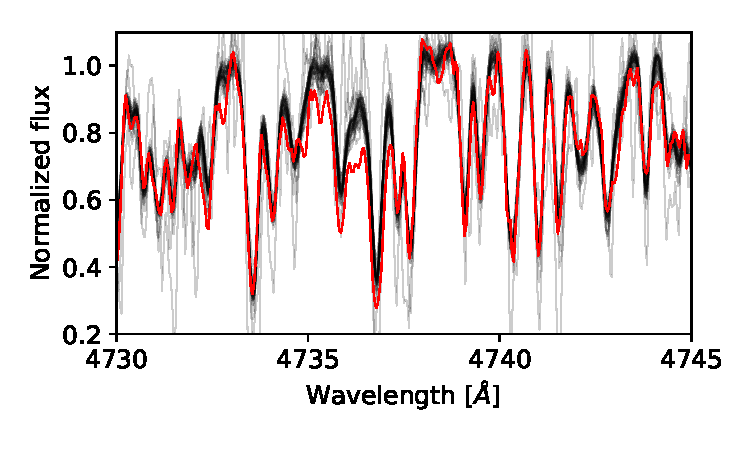
\includegraphics[width=0.6\textwidth]{150206004301057_tsne_close30.pdf}
	\caption{Spectral comparison between one of the detected carbon-enhanced stars in red and its 30 closest neighbours in the t-SNE projection shown as black curves. Enhancement in the spectrum was probably not sufficiently distinct and was dominated by the spectral noise. Therefore the spectrum was placed among other physically similar spectra without visible enhancement.}
	\label{fig:tsne_30close}
\end{figure}

\section{Candidate characteristics}
\label{sec:analysis_cemp}
The final list of detected carbon-enhanced stars consists of 918 stars, corresponding to 993 spectra detected by at least one of the described methods. Among them, 63 stars were observed and identified at least twice and up to a maximum of four times. Those identifications belong to repeated observations that were performed at different epochs. Because not all of the observed spectra were considered in the classification procedure (due to the limitations described in Section \ref{sec:classification_cemp}) this is not the final number of stars with repeated observations. By searching among the complete observational data set, the number of carbon-enhanced stars with repeated observations increases to 90.

Out of those 90 stars, every repeated observation of 56 stars was classified as being carbon-enhanced. In total, we detected $76.5$~\% of the carbon-enhanced spectra among repeated observations where at least one of the repeats have been classified as having enhanced carbon features in its spectrum. The unclassified instances usually have a low SNR value that could decrease their similarity value towards other carbon-enhanced stars in the t-SNE analysis or have incorrect stellar parameters and were therefore compared to an incorrect median spectrum during the supervised analysis.

\subsection{Radial velocity variations}
\label{sec:binaries}
With repeated observations in the complete observational data set, we can look into measured radial velocities and investigate a fraction of possible variables that should be high or even close to 100~\% for certain types of carbon-enhanced objects \citet{2016ApJ...826...85S}. Taking into account all of the repeated observations in our data set and not just the repeats among the identified spectra, 52 out of 90 stars show a minimum velocity change of $0.5$~\kms (70 stars with minimum change of $0.25$ \kms) and a maximum of $45$~\kms in different time spans ranging from days to years. The detailed distribution is presented by Figure \ref{fig:rv_rep_dist}. The threshold was selected in a such way to be significantly larger than the estimated typical accuracy of $\sim0.1$~\kms as determined for the \Gh\ radial velocities by \citet{2018arXiv180406344Z}.

Any radial velocity change can hint at the presence of a secondary member or at intrinsic stellar pulsation \cite{2002AA...390..987B, 2010JApA...31..177L, 2012A&A...544A..10B}, as carbon-enhanced stars are found among all long-period variable classes (Mira, SRa, and SRb  \cite{2013A&A...553A..93B, 2014A&A...568A.100B}). Follow-up observations are needed to determine their carbon sub-class and subsequently, the reason behind variations of radial velocity.

\begin{figure}
	\centering
	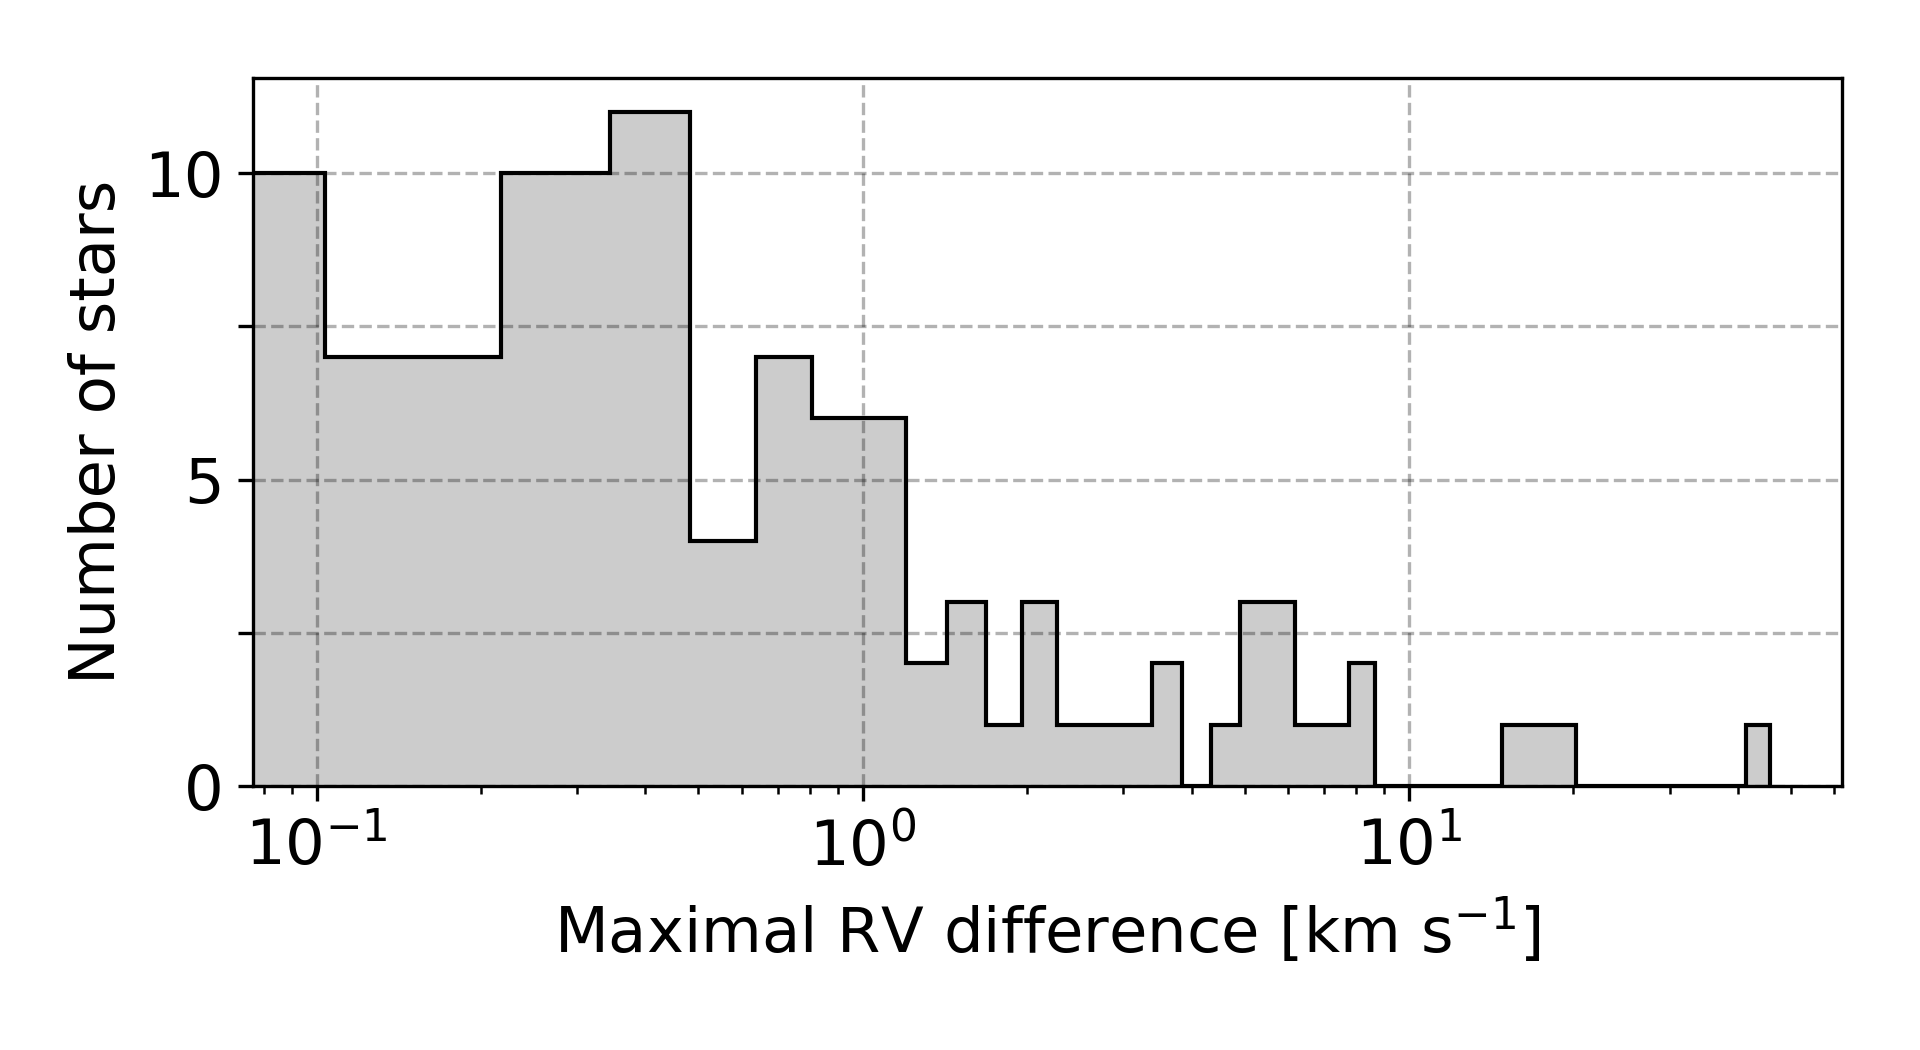
\includegraphics[width=0.6\textwidth]{rv_rep_dist.png}
	\caption{Distribution of maximal velocity change between repeated observations of the stars that were classified as carbon-enhanced.}
	\label{fig:rv_rep_dist}
\end{figure}
% TODO Kot rečeno spodaj, tu dodaš še primerjalni graf za ne CE zvezde enakih spektralnih tipov - razlika naj bi pokazala, da so RV variacije CE zvezd signifikantne.

Visual inspection of variable candidates revealed that none of them shows obvious multiplications of spectral absorption lines, a characteristic of a double-lined binary system. Therefore we can conclude that none of them is a binary member in which both components are of comparable luminosity, and a difference between their projected radial velocities is high enough to form a double-lined spectrum. From our simulations with median spectra, such line splitting becomes visually evident at the velocity difference of $\sim$14~\kms. If the components do not contribute the same amount of flux, the minimal difference increases to $\sim$20~\kms.

The chemical peculiarity of a dwarf carbon-enhanced star (dC) that exhibits enhancement of C$_2$ in its spectra could be explained by its interaction with a primary star in a binary system \cite{2018ApJ...856L...2M}. Chemically enhanced material is thought to be accreted from the evolved AGB companion. Less than thirty of such systems that show signs of the existence of an invisible evolved companion who might have enriched a dC by the carbon have been identified spectroscopically to date \cite{1986ApJ...300..314D, 2018ApJ...856L...2M, 2018MNRAS.479.3873W}. This low number of confirmations gave us the possibility to greatly increase the list with every additional confirmed object. The only detected dC star (for criteria see Section \ref{sec:cannon_params}) with repeated observations shows that its radial velocity is unchanged on the order of $0.1$~\kms\ during the two years between consecutive observations. Hence, it cannot be classified as a possible binary system from those two observations alone. The lack of clear evidence for binarity among dC stars, especially among the most metal-poor, can also be explained by another enrichment mechanism. \citet{2018MNRAS.477.3801F} showed that a substantial fraction of those stars belongs to the halo population based on their kinematics information. We performed similar analysis in Section \ref{sec:cemp_cemp} that is supported by Figures \ref{fig:orbits_vxvyvz} and \ref{fig:orbits_zmax}. Combined with the results of \citet{2016ApJ...833...20Y} that classified the prototype dC star \mbox{G 77-61} as a CEMP-no star, that is known to have intrinsically low binarity fraction \cite{2014MNRAS.441.1217S, 2016A&A...586A.160H}, their carbon-enhancement may be of a primordial origin.

\subsection{Stellar parameters}
\label{sec:cannon_params}
For the analysis of stellar parameters, we used values determined by \TC\ data interpolation method that was trained on actual observed HERMES spectra. To exclude any potentially erroneous parameter, we applied a strict flagging rule of \texttt{flag\_cannon}=0 (extensive description of the flagging procedure can be found in \citet{buder2018}), thus obtaining a set of 347 objects with trustworthy stellar parameters. Such a large percentage of flagged objects could be attributed to their nature as an additional elemental enhancement that we are looking for might not be a part of the training set. A raised quality flag would hint that the spectrum is different from any other in the training set or that the fit is uncertain and has a large $\chi^2$. Therefore flagged parameters have to be used with care, especially on the border of, and outside the training set.

The majority (338) of the unflagged detected objects are giants, and only nine are confirmed to be dwarf stars based on their spectroscopic stellar parameters (Figure \ref{fig:kiel_plot}).

\begin{figure}
	\centering
	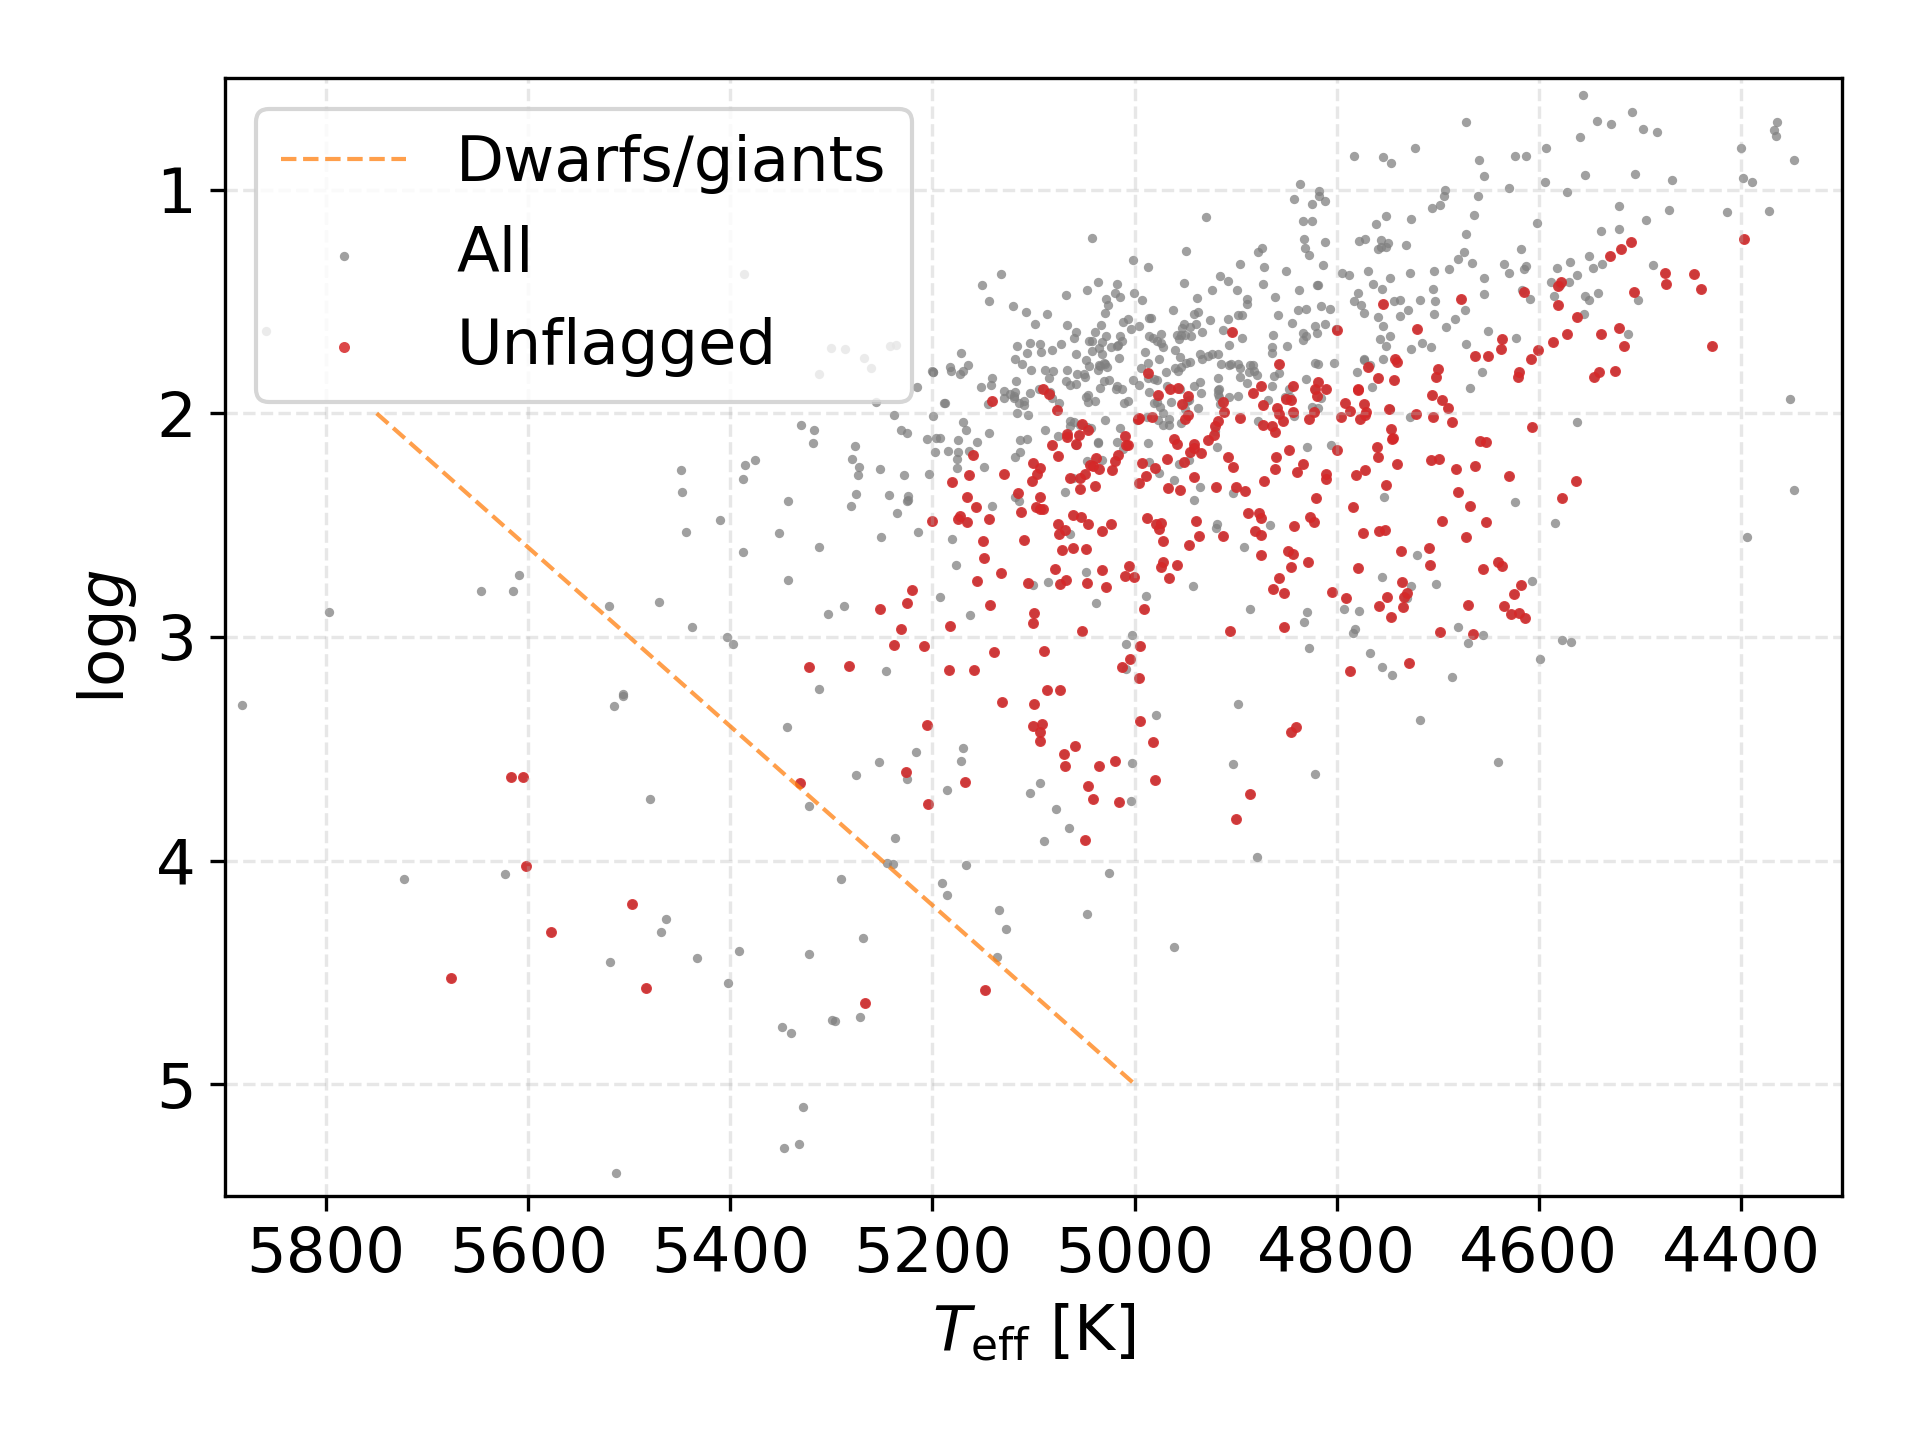
\includegraphics[width=0.6\textwidth]{Kiel_diagram.png}
	\caption{Kiel diagram for a subset of 338 detected carbon-enhanced stars with valid stellar parameters in red. Uncertain positions of flagged stars are shown with grey dots. Dashed orange line illustrates the border between giants and dwarfs.}
	\label{fig:kiel_plot}
\end{figure}

\subsection{S-process elements}
\label{sec:sprocess}
Focusing on a spectral signature of the detected objects inside and outside the t-SNE selected clump (Figure \ref{fig:tsne_plot}) we can further investigate which spectral feature might have contributed to their separation. The distributions of their abundances in Figure \ref{fig:sprocess_hist} and strength of spectral features corresponding to the same elements in Figure \ref{fig:sprocess_spectrum} hints to an enhancement of s-process elements among stars inside the selected clump. The abundance difference is slightly  different for every elements. In general the abundance peaks are separated for about $1$~dex This additional enhancement might be another reason, besides the carbon enhancement, for the algorithm to cluster all of those stars as being different from the majority of spectra.

\begin{figure}
	\centering
	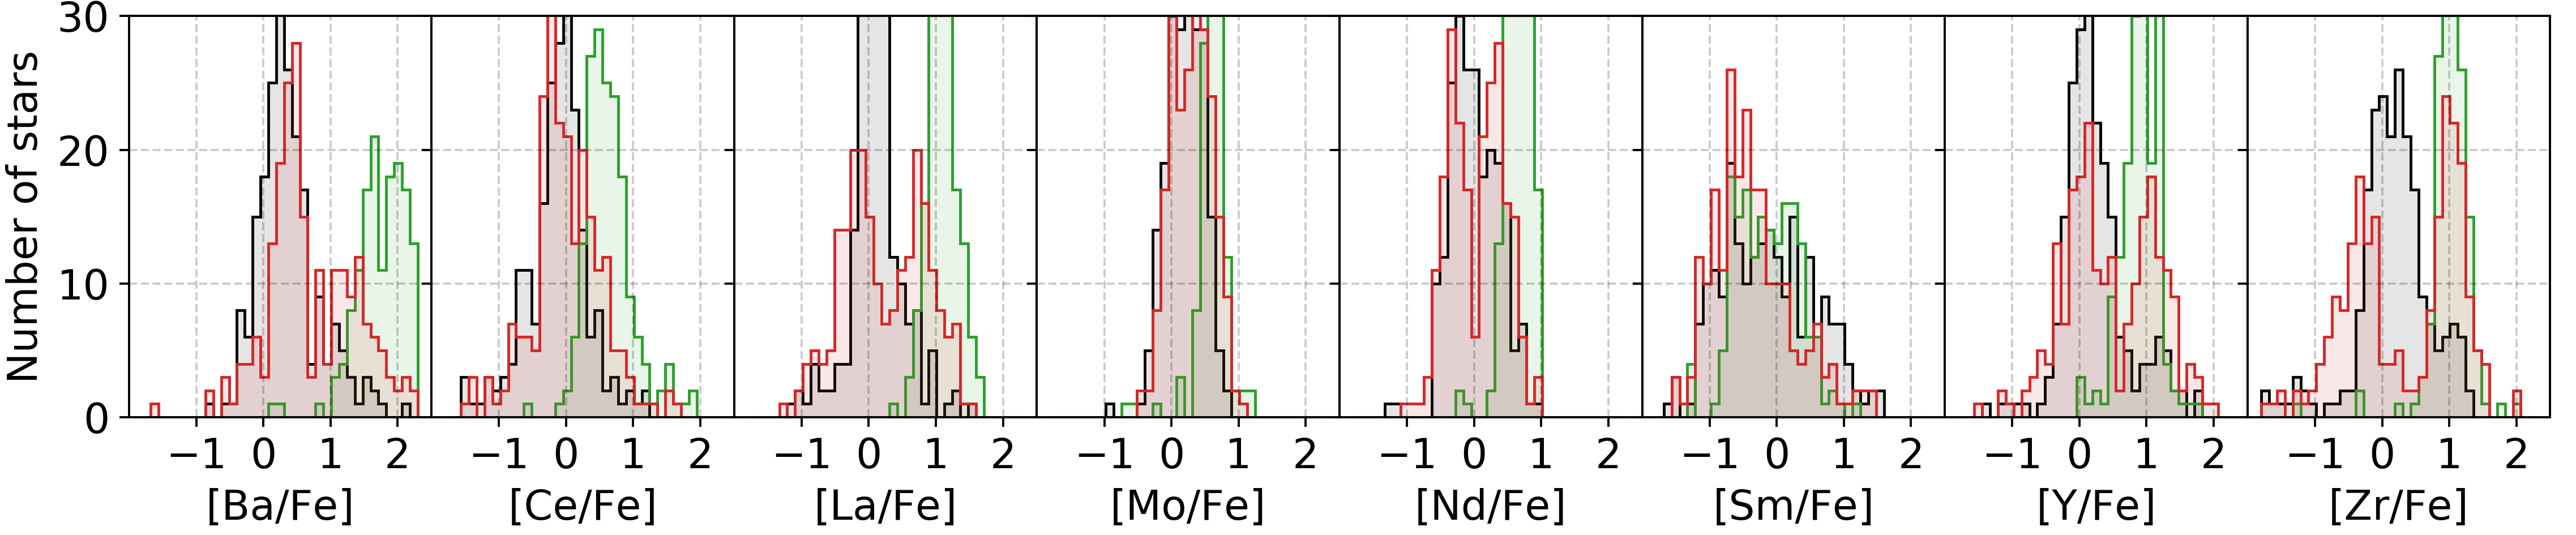
\includegraphics[width=\textwidth]{sprocess_hist.png}
	\caption{Distribution of s-process element abundances for stars in three different groups. The most enhanced group in green represent carbon-enhanced stars located in the t-SNE selected clump of stars. The red distribution presents all other detections that are placed around the projection, and outside the clump. As a control group, the same distribution in black is shown for their closest t-SNE neighbours, therefore the black and red distribution contain an equal number of objects. No abundance quality flags were used to limit abundance measurements.}
	\label{fig:sprocess_hist}
\end{figure}

\begin{figure}
	\centering
	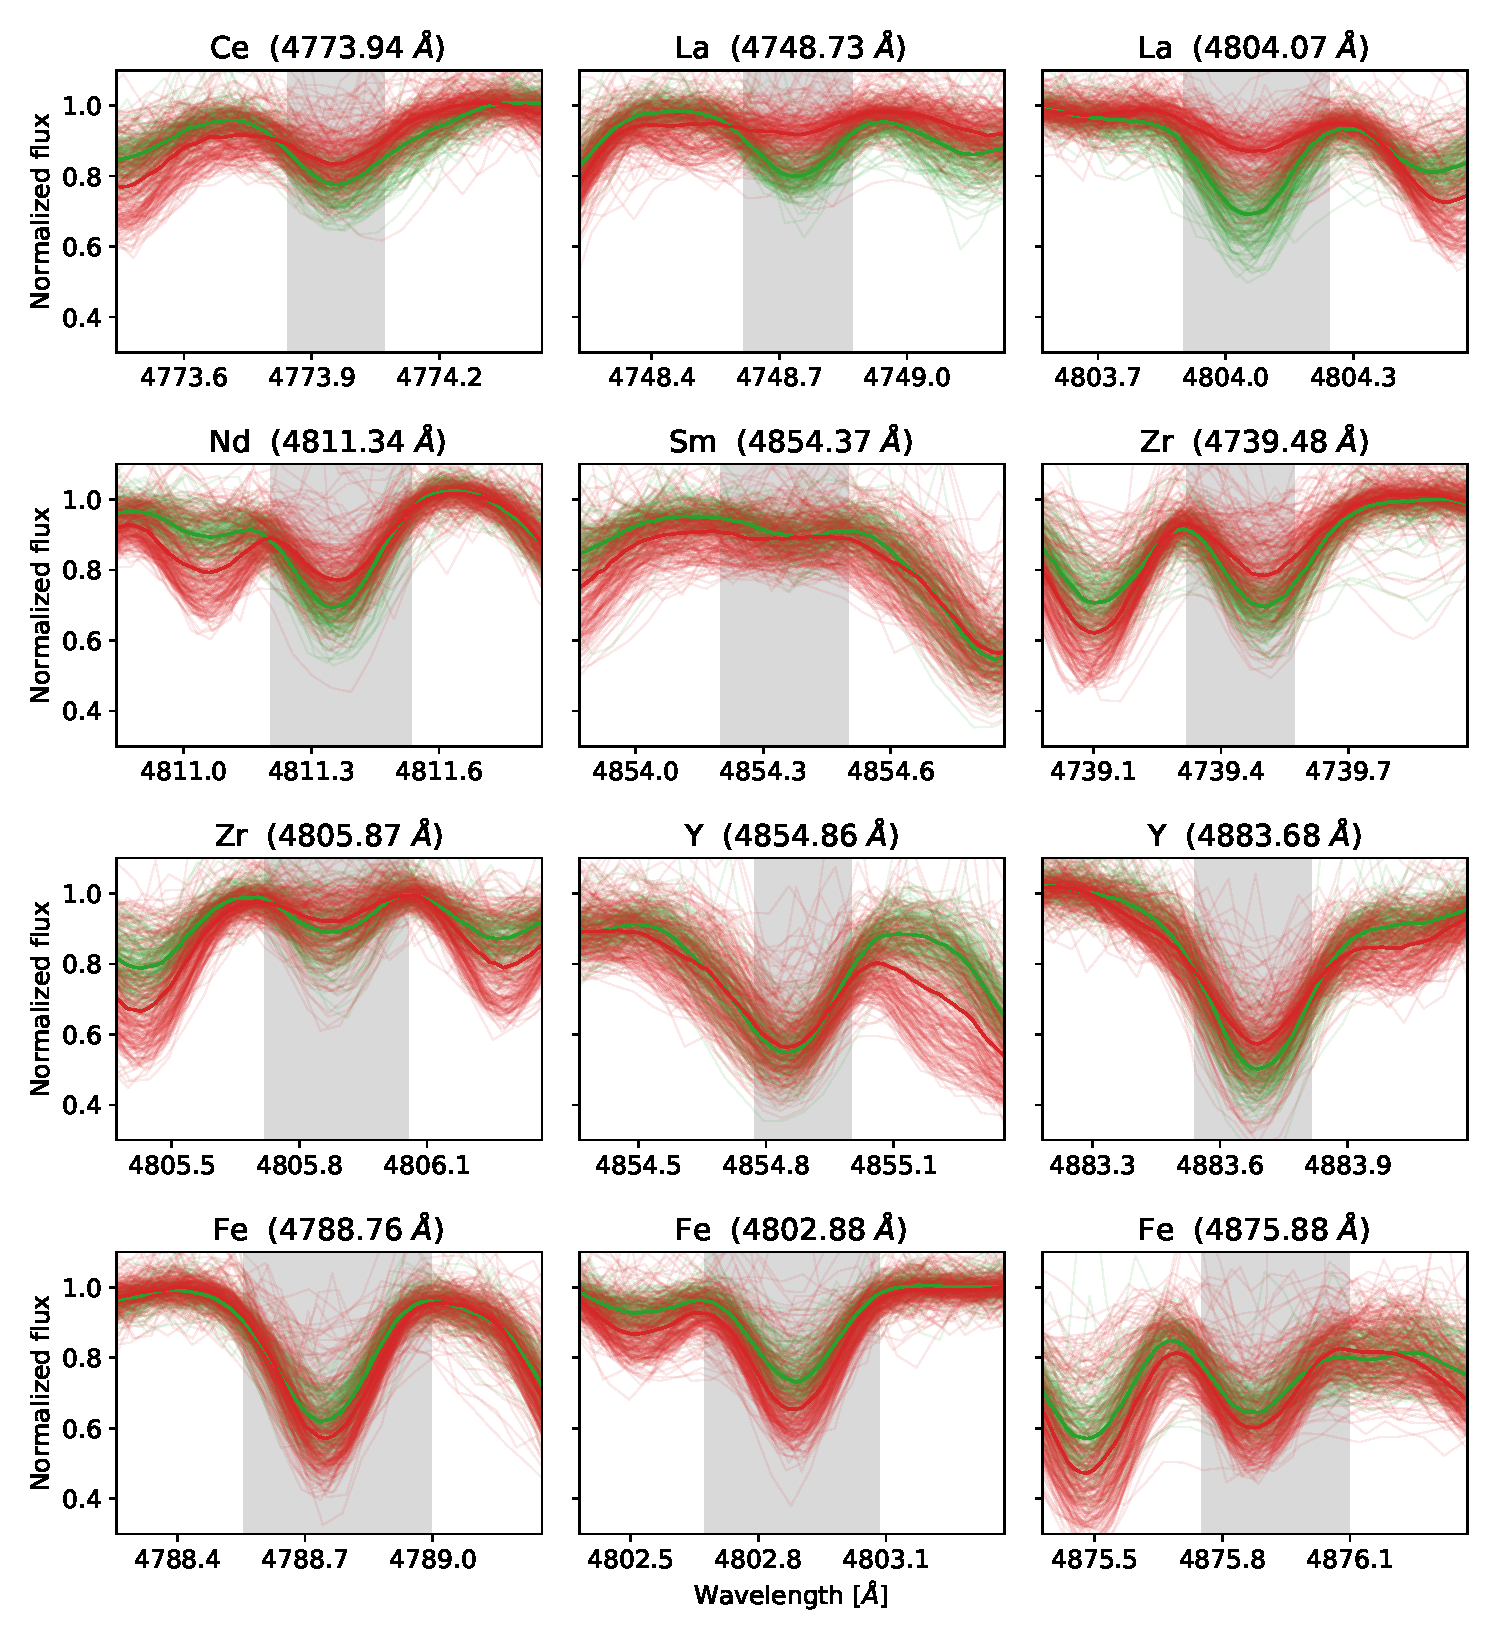
\includegraphics[width=\textwidth]{sprocess_spectra.pdf}
	\caption{Spectral subset around the absorption features in the blue arm that were used to determine abundances of Fe and s-process elements. Same colour coding is used as in Figure \ref{fig:sprocess_hist}. Spectra inside the t-SNE determined clump are shown in red, and outside it in green. Median of all spectra is shown with a bold line of the same colour. The shaded area gives the wavelength range considered in the computation of abundances. The abundance difference is the result of green spectra having lower Fe enhancement and higher enhancement (deeper absorption lines) of s-process elements.}
	\label{fig:sprocess_spectrum}
\end{figure} 

\subsection{Lithium abundance}
\label{sec:lithium}
The derivation of elemental abundances for known carbon-enhanced stars has shown that some of them can exhibit strongly enhanced levels of Li in their atmosphere \cite{1991A&A...245L...1A}. Lithium is thought to be produced by hot-bottom burning \cite{1974ApJ...187..555S} and brought to the surface from the stellar interior. Investigation of the Li line at 6707~\AA\ revealed 32 of such stars. Their spectra, centred around the Li feature, show a greatly varying degree of absorption in Figure \ref{fig:li_abund}.

\begin{figure}
	\centering
	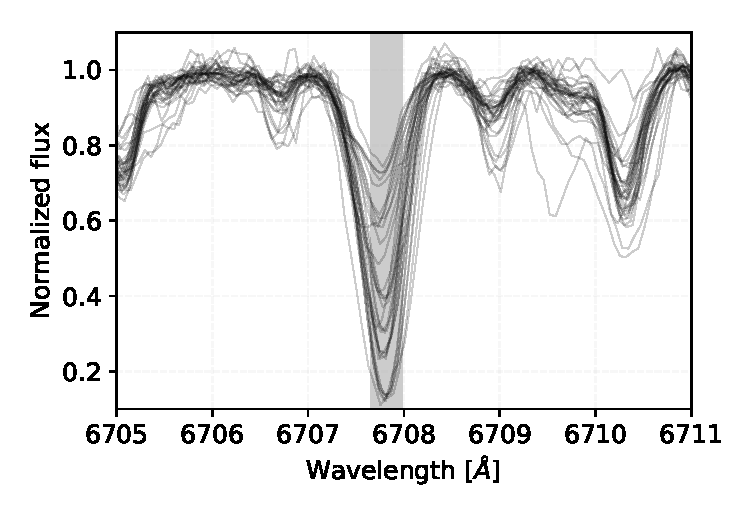
\includegraphics[width=0.6\textwidth]{li_string_ch.pdf}
	\caption{Spectral subset of 32 lithium-rich carbon-enhanced stars among the identified stars. The highlighted wavelength region is used by \TC\ to determine the lithium abundance of a star.}
	\label{fig:li_abund}
\end{figure}

\subsection{Sub-classes}
\label{sec:subclasses}
Following a revision of the original MK classification \cite{1941ApJ....94..501K} introduced by \citet{1996ApJS..105..419B}, carbon stars are separated into five different classes named \mbox{C-H}, \mbox{C-R}, \mbox{C-J}, \mbox{C-N}, and Barium stars. Of all the spectral indices proposed for the spectral classification, we are only able to measure a small part of Swan C$_2$ bands and Ba II line at 6496~\AA. For a more detailed classification of detected objects into proposed classes, we would need to carry out additional observations with a different spectroscopic setup to cover all the significant features. 

Additionally, the features caused by the $^{13}$C$^{12}$C molecule are strongly enhanced only for a handful of spectra in our data set, therefore we did not perform any isotopic ratio analysis or identification of possible C-J objects, which are characterised by strong Swan bands produced by the heavier isotopes.

According to the abundance trends presented in Section \ref{sec:sprocess} and the classification criteria defined by \citet{1996ApJS..105..419B}, we could argue that the stars selected from the t-SNE projection belong to the C-N sub-class. Their s-process elements are clearly enhanced over solar values (see Figure \ref{fig:sprocess_hist}), but the actual values should be treated with care as they are mostly flagged by \TC (having quality flag \texttt{flag\_cannon}~>~0). This uncertainty might come from the fact that the training set does not cover carbon-enhanced stars and/or stars with such enhancement of s-process elements.

\subsection{Match with other catalogues}
In the literature we can find numerous published catalogues of carbon-enhanced (CH) stars \cite{2001A&A...375..366C, 2001BaltA..10....1A,2016ApJS..226....1J} and CEMP stars \cite{2007ApJ...658..367K, 2010A&A...509A..93M, 2010AJ....139.1051P, 2014ApJ...797...21P, 2015A&A...581A..22A, 2017yCat..18330020Y} observed by different telescopes and analysed in inhomogeneous ways. Most of those analyses were also performed on spectra of lower resolving power than the HERMES, therefore some visual differences are expected for wide molecular bands. By matching published catalogues with the GALAH observations that were analysed by our procedures, we identified 44 stars that matched with at least one of the catalogues. Of these, 28 were found in CH catalogues and 16 in CEMP catalogues.

From the stars recognised as CEMPs in the literature, we were able to detect only 1 star using the described methods. Visual assessment of the diagnostic plots provided by our analysis pipeline proved that the remaining 15 CEMP matches do not expresses any observable carbon enhancement in Swan bands and were therefore impossible to detect with the combination of our algorithms. The reason for this difference between our and literature results might be in the CEMP selection procedure employed by the aforementioned literature. Every considered study selects their set of interesting stars from one or multiple literature sources based on values of \Meh\ and \Cfe\ that were measured from the atomic spectral lines and not molecular lines. 

The match is larger in the case of CH matches, where we were able to confirm 11 out of 33 possible matched carbon-enhanced stars. As the observed molecular bands are prominent features in the spectra, we explored possible reasons for our low detection rate. Visual inspection of spectra for the remaining undetected matched stars proved that they also show no or barely noticeable carbon enhancement in the spectral region of Swan bands, therefore reason must lie in the detection procedures used in the cited literature. \citet{2001A&A...375..366C} used low-resolution spectra to evaluate enhancement of C$_2$ and CN bands. The results are also summarised in their electronic table. In here, all of our undetected stars are marked to contain enhanced CN bands but no C$_2$ bands. Combining this with Figure \ref{fig:ch_xmatch} we speculate that those stars occupy a narrow range of parameter space where C$_2$ is not expressed and therefore undetectable in the HERMES spectra. 

Number of successfully detected stars matched between the surveys could also be influenced by different excitation temperatures of analysed carbon-rich molecules. Frequently studied photometric G-band (centred at 4640~\AA\ and FWHM of 1200~\AA), that is not present in our spectra, covers a spectral region rich in CH molecule features whose temperature dependence is different than for a C$_2$ molecule. Presence of those bands is identified by classifying a carbon-enhanced star into C-H sub-class (see Section \ref{sec:subclasses}). As we detected all C-H stars identified by \citet{2016ApJS..226....1J}, that are also present in the GALAH data set, we are unable to discuss about the selection effect in the \Teff\ range between $\sim$5100 and $\sim$5300~K where those three stars were found.

\begin{figure}
	\centering
	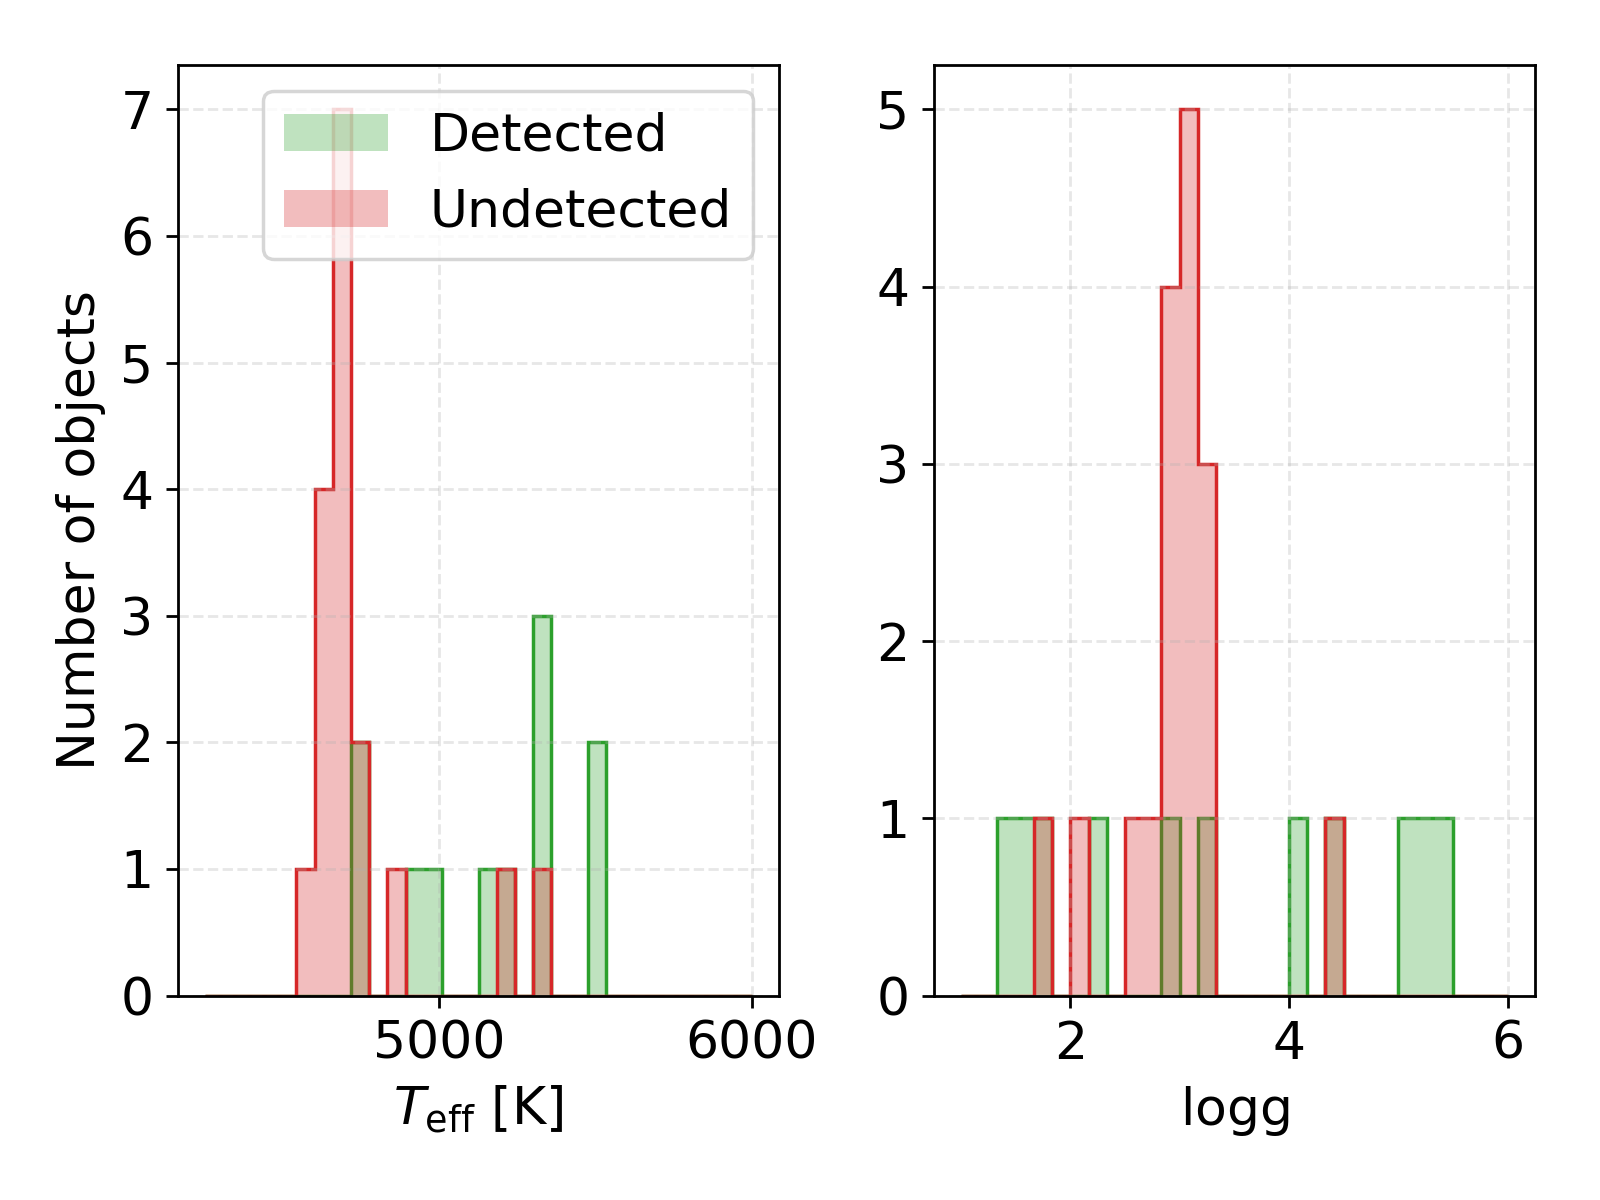
\includegraphics[width=0.6\textwidth]{ch_comb.png}
	\caption{Comparison between the stellar parameters of detected (green histogram) and undetected (red histogram) carbon-enhanced stars found in literature.}
	\label{fig:ch_xmatch}
\end{figure}

The position of all stars matched with the literature is also visualised on the \mbox{t-SNE} projection in Figure \ref{fig:tsne_ref_ch}, where it can be clearly seen that they lie outside the selected clump with identified carbon enhancement and are strewn across the projection. Close inspection of spectra that are spatially near the aggregation of CEMP stars from the literature, revealed no visible carbon enhancement. The enhancement is present neither in form of molecular bands nor expressed as stronger atomic carbon line. They therefore are indistinguishable from other metal-poor stars with similar physical parameters.

\begin{figure}
	\centering
	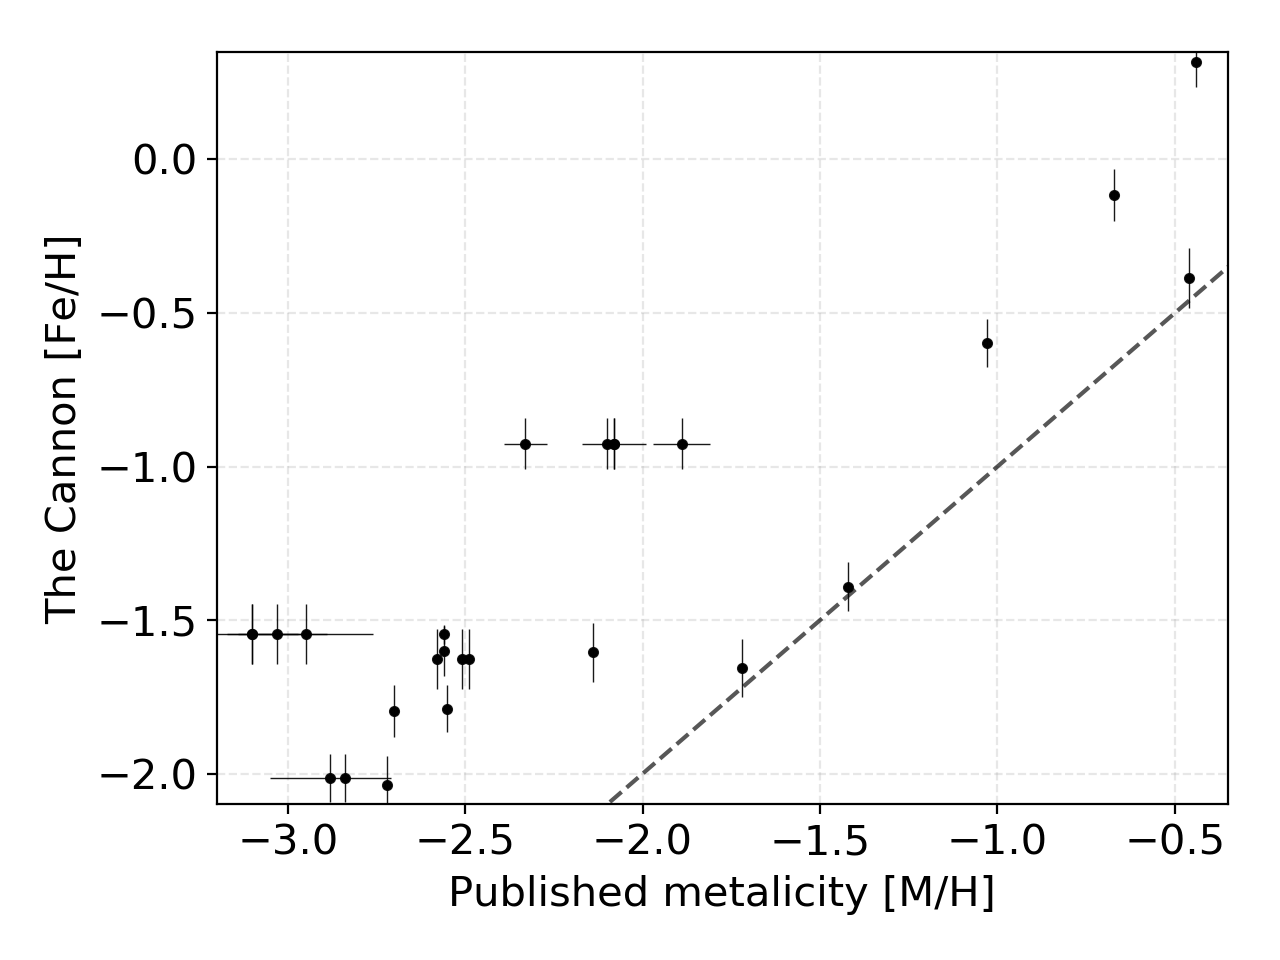
\includegraphics[width=0.6\textwidth]{cemps_meh_feh.png}
	\caption{Correlation between published metallicities and \TC\ iron abundance for the stars that were classified as CEMPs in the literature. As some of those stars were taken from multiple literature sources, we also have multiple determinations of \Meh\ for them. This can be identified as horizontal clusters of dots at different \Meh, but with the same \Feh. Where available, uncertainties of parameters are shown. The dashed line follows a 1:1 relation.}
	\label{fig:cemps_feh}
\end{figure}

\section{Metal-poor candidates}
\label{sec:cemp_cemp}
CEMP stars are defined in the literature as having low metallicity \Meh \textless $-1$ and strong carbon enrichment \Cfe \textgreater $+1$. In the scope of this analysis, we assume that our measurement of \Feh\ is a good approximation for the metallicity. To be sure about this we compared \Meh\ values of CEMP stars found in the literature and \Feh\ derived by \TC\ for the same stars. The relation between them is shown in Figure \ref{fig:cemps_feh}. We see that our values start deviating from the published values at metallicities bellow $-1.5$. Bellow that threshold the differences are in the range of $\sim1$ dex, but the same trend is obvious for both data sets. General offset between \Feh\ and \Meh\ is expected as the later gives abundance information of all elem and not just iron. Uncertainty of the published \Meh, derived from multiple sources, can reach up to $0.5$. 

\begin{figure}
	\centering
	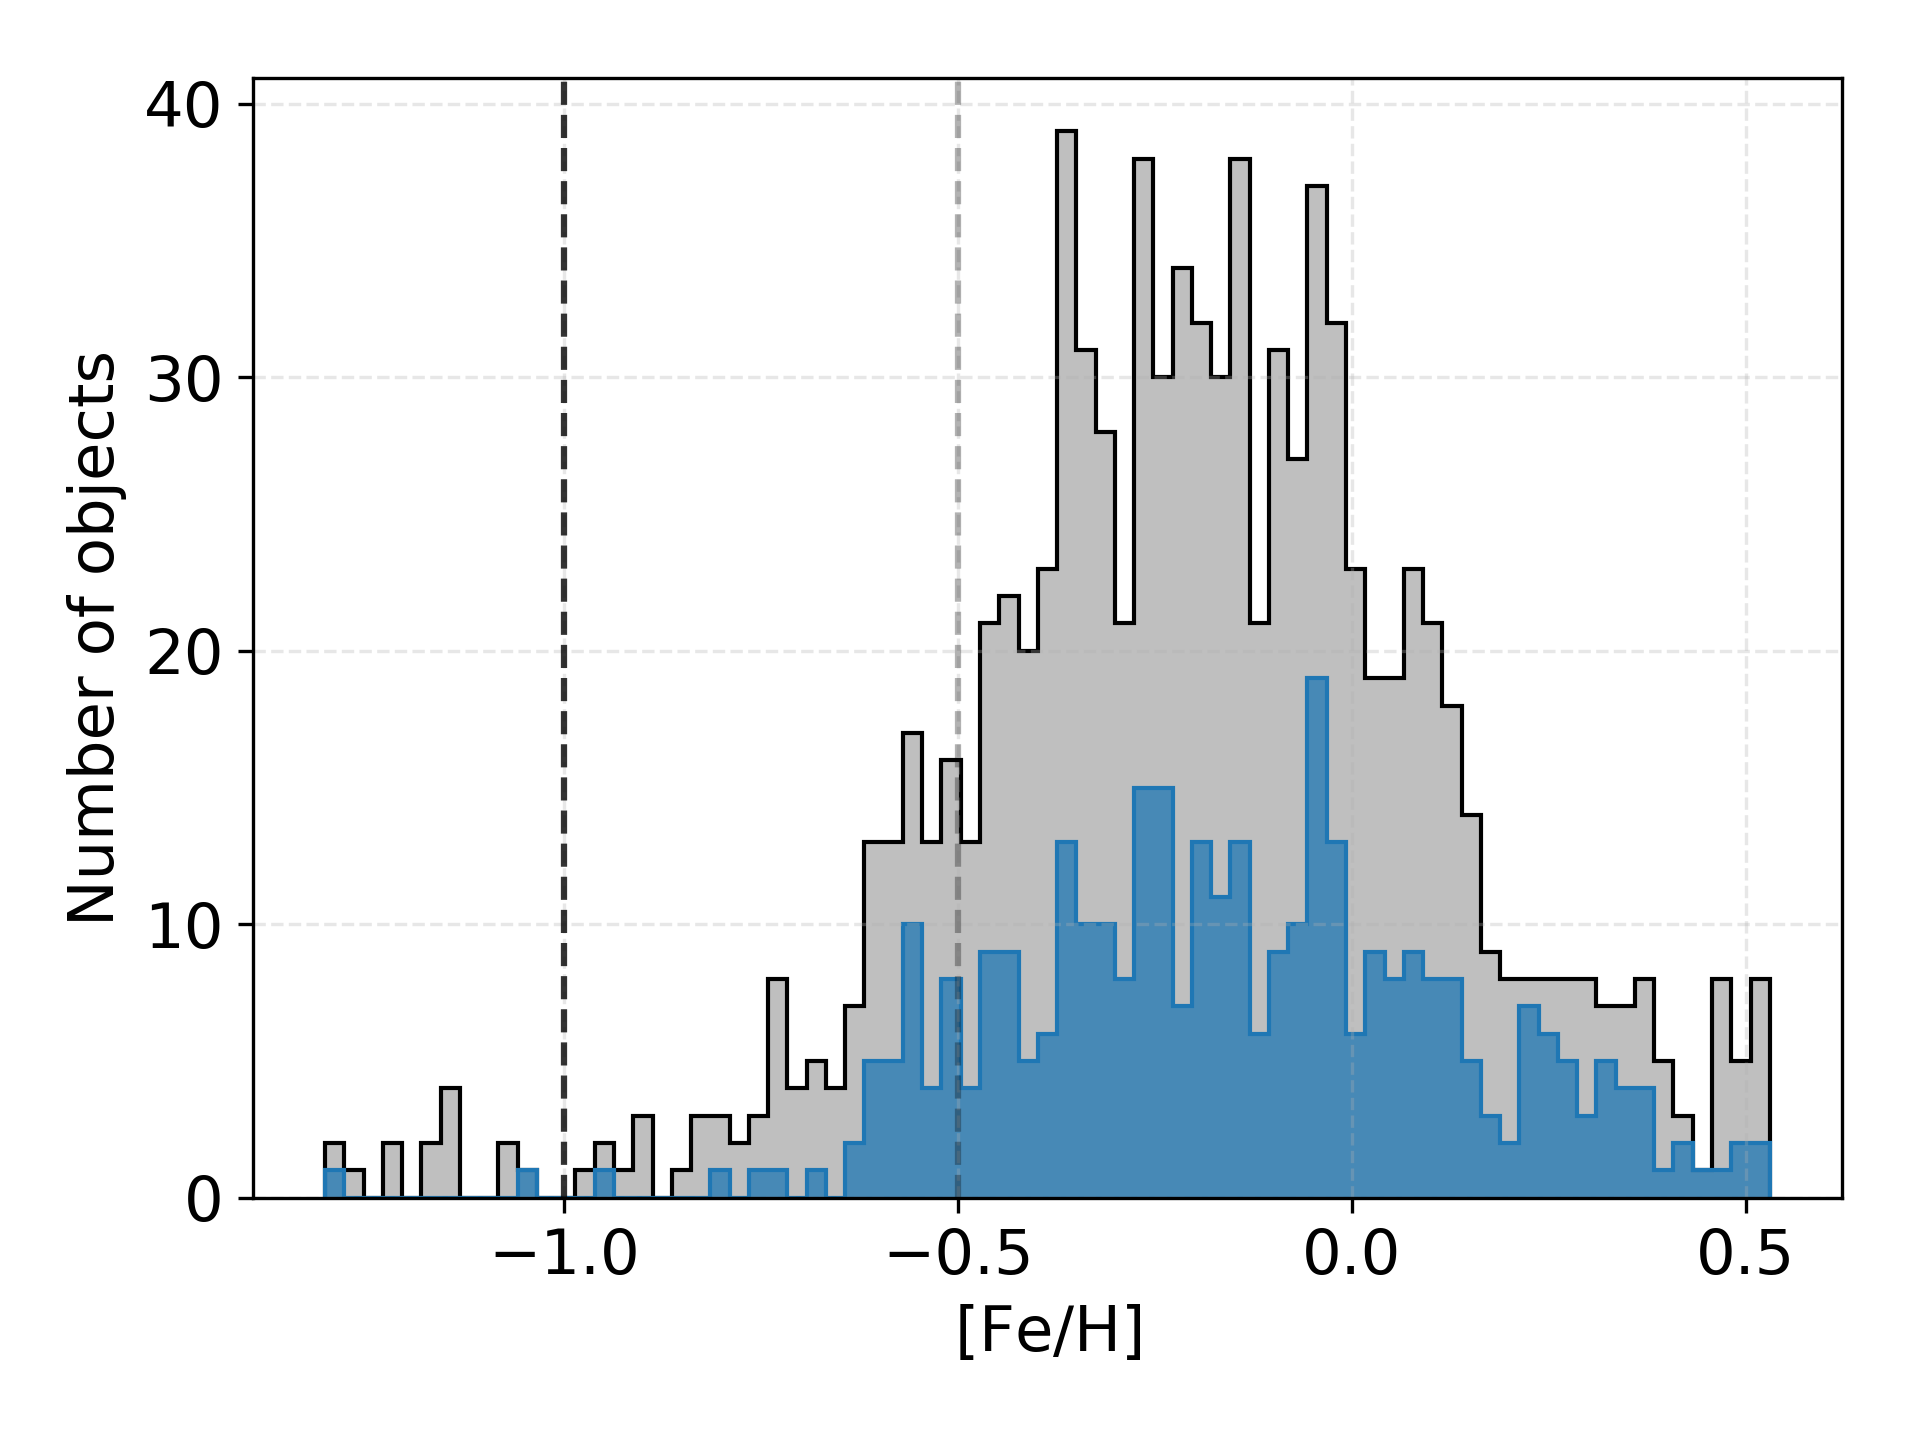
\includegraphics[width=0.6\textwidth]{Fe_H_cannon.png}
	\caption{Histogram of \Feh\ for detected carbon-enhanced stars with valid \TC\ stellar parameters in blue and for every detected carbon-enhanced star in grey. Two vertical lines are located at iron abundances of $-1.0$ and $-0.5$.}
	\label{fig:feh_candidates}
\end{figure}

Taking unflagged \TC\ parameters and abundances of the detected objects we can determine possible CEMP candidates among our sample. As also shown by Figure \ref{fig:feh_candidates} our set of carbon-enhanced stars consists of 41 objects with \Feh \textless $-0.5$ and 2 objects with \Feh \textless $-1.0$. If we also include potentially incorrect parameters, the number of objects with \Feh \textless $-1.0$ increases to 28, which is equal to $2.8$~\% of detected carbon-enhanced spectra. In any case, none of them has a valid determination of carbon abundance. Analysing HERMES spectra in order to determine carbon abundance is difficult because the automatic analysis is based on only one very weak atomic absorption line that is believed to be free of any blended lines. Consequently, we are also not able to measure the \CO\ abundance ratio, as a majority of determined \Cfe\ abundances is flagged as unreliable. Complementary observations are needed to determine the abundance and confirm suggested CEMP candidates.

A low number of metal-poor candidates could also be explained by the specification of the HERMES spectrograph as its spectral bands were not selected in a way to search for and confirm most metal-poor stars. With the release of {\it Gaia} DR2 data \cite{2018A&A...616A...1G}, stars low/high-metallicity could also be compared with their Galactic orbits. To determine the distribution of detected stars among different Galactic components, we performed an orbital integration in \texttt{MWPotential2014} Galactic potential using the \texttt{galpy} package \cite{2015ApJS..216...29B}. In order to construct a complete 6D kinematics information, {\it Gaia} parallax and proper motion measurements were supplemented with the GALAH radial velocities. Results shown in Figure \ref{fig:orbits_zmax} suggest that our CEMP candidates could belong to two different components of the Galaxy. Stars with maximal $z$~<~4~kpc most probably belong to the thick disk and stars with $z$~>~5~kpc to the halo population that is inherently metal-poor. This is also supported by their angular momentum in the same plot and their Galactic velocities shown in Figure \ref{fig:orbits_vxvyvz}.

\begin{figure}
	\centering
	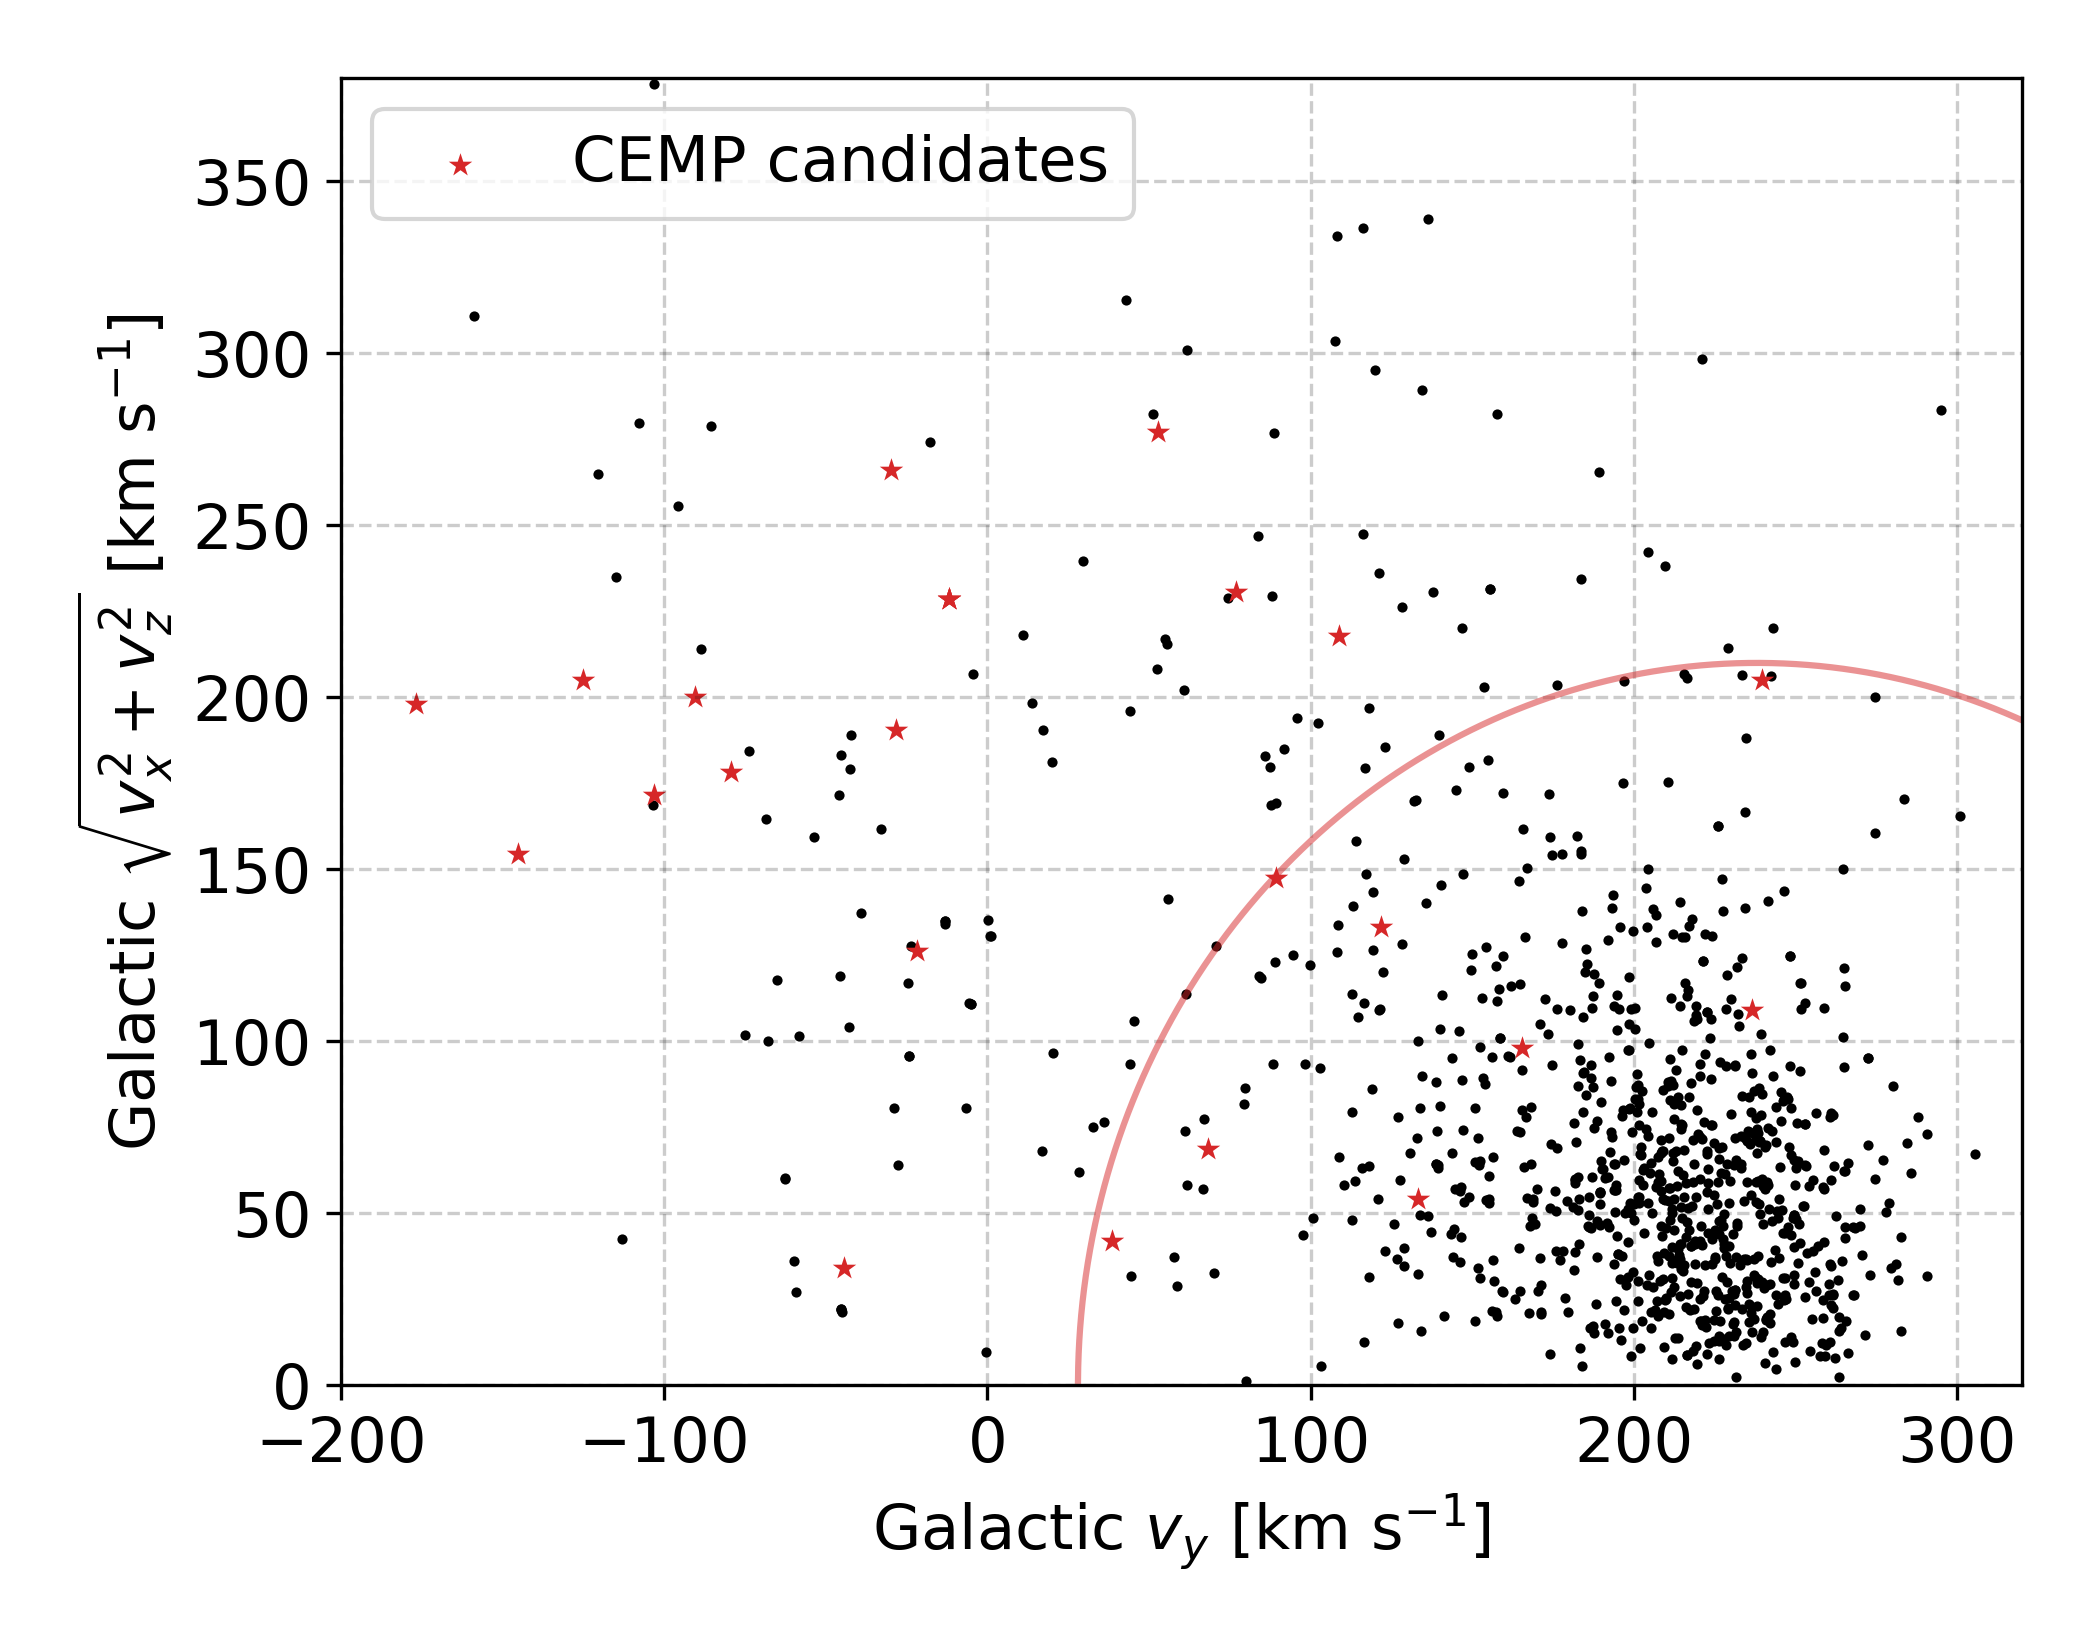
\includegraphics[width=0.6\textwidth]{carbon_orbits_vy_vxvz.png}
	\caption{Toomre diagram used to identify possible local halo stars among our detected carbon-enhanced stars, especially CEMP candidates. Halo stars in this diagram are located above the red circular line, satisfying the velocity condition $\left|\mathbf{v} - \mathbf{v_{LSR}} \right|$~>~210~\kms\ (the threshold taken from \citet{2018ApJ...860L..11K}). CEMP candidates are marked with star symbols.}
	\label{fig:orbits_vxvyvz}
\end{figure}

When looking at the distribution of \Feh\ for the complete set of observed stars, we find a comparable distribution as for carbon-enhanced stars. Similarly, about $1.8$~\% of stars are found to be metal-poor with \Feh \textless $-1.0$.

\begin{figure}
	\centering
	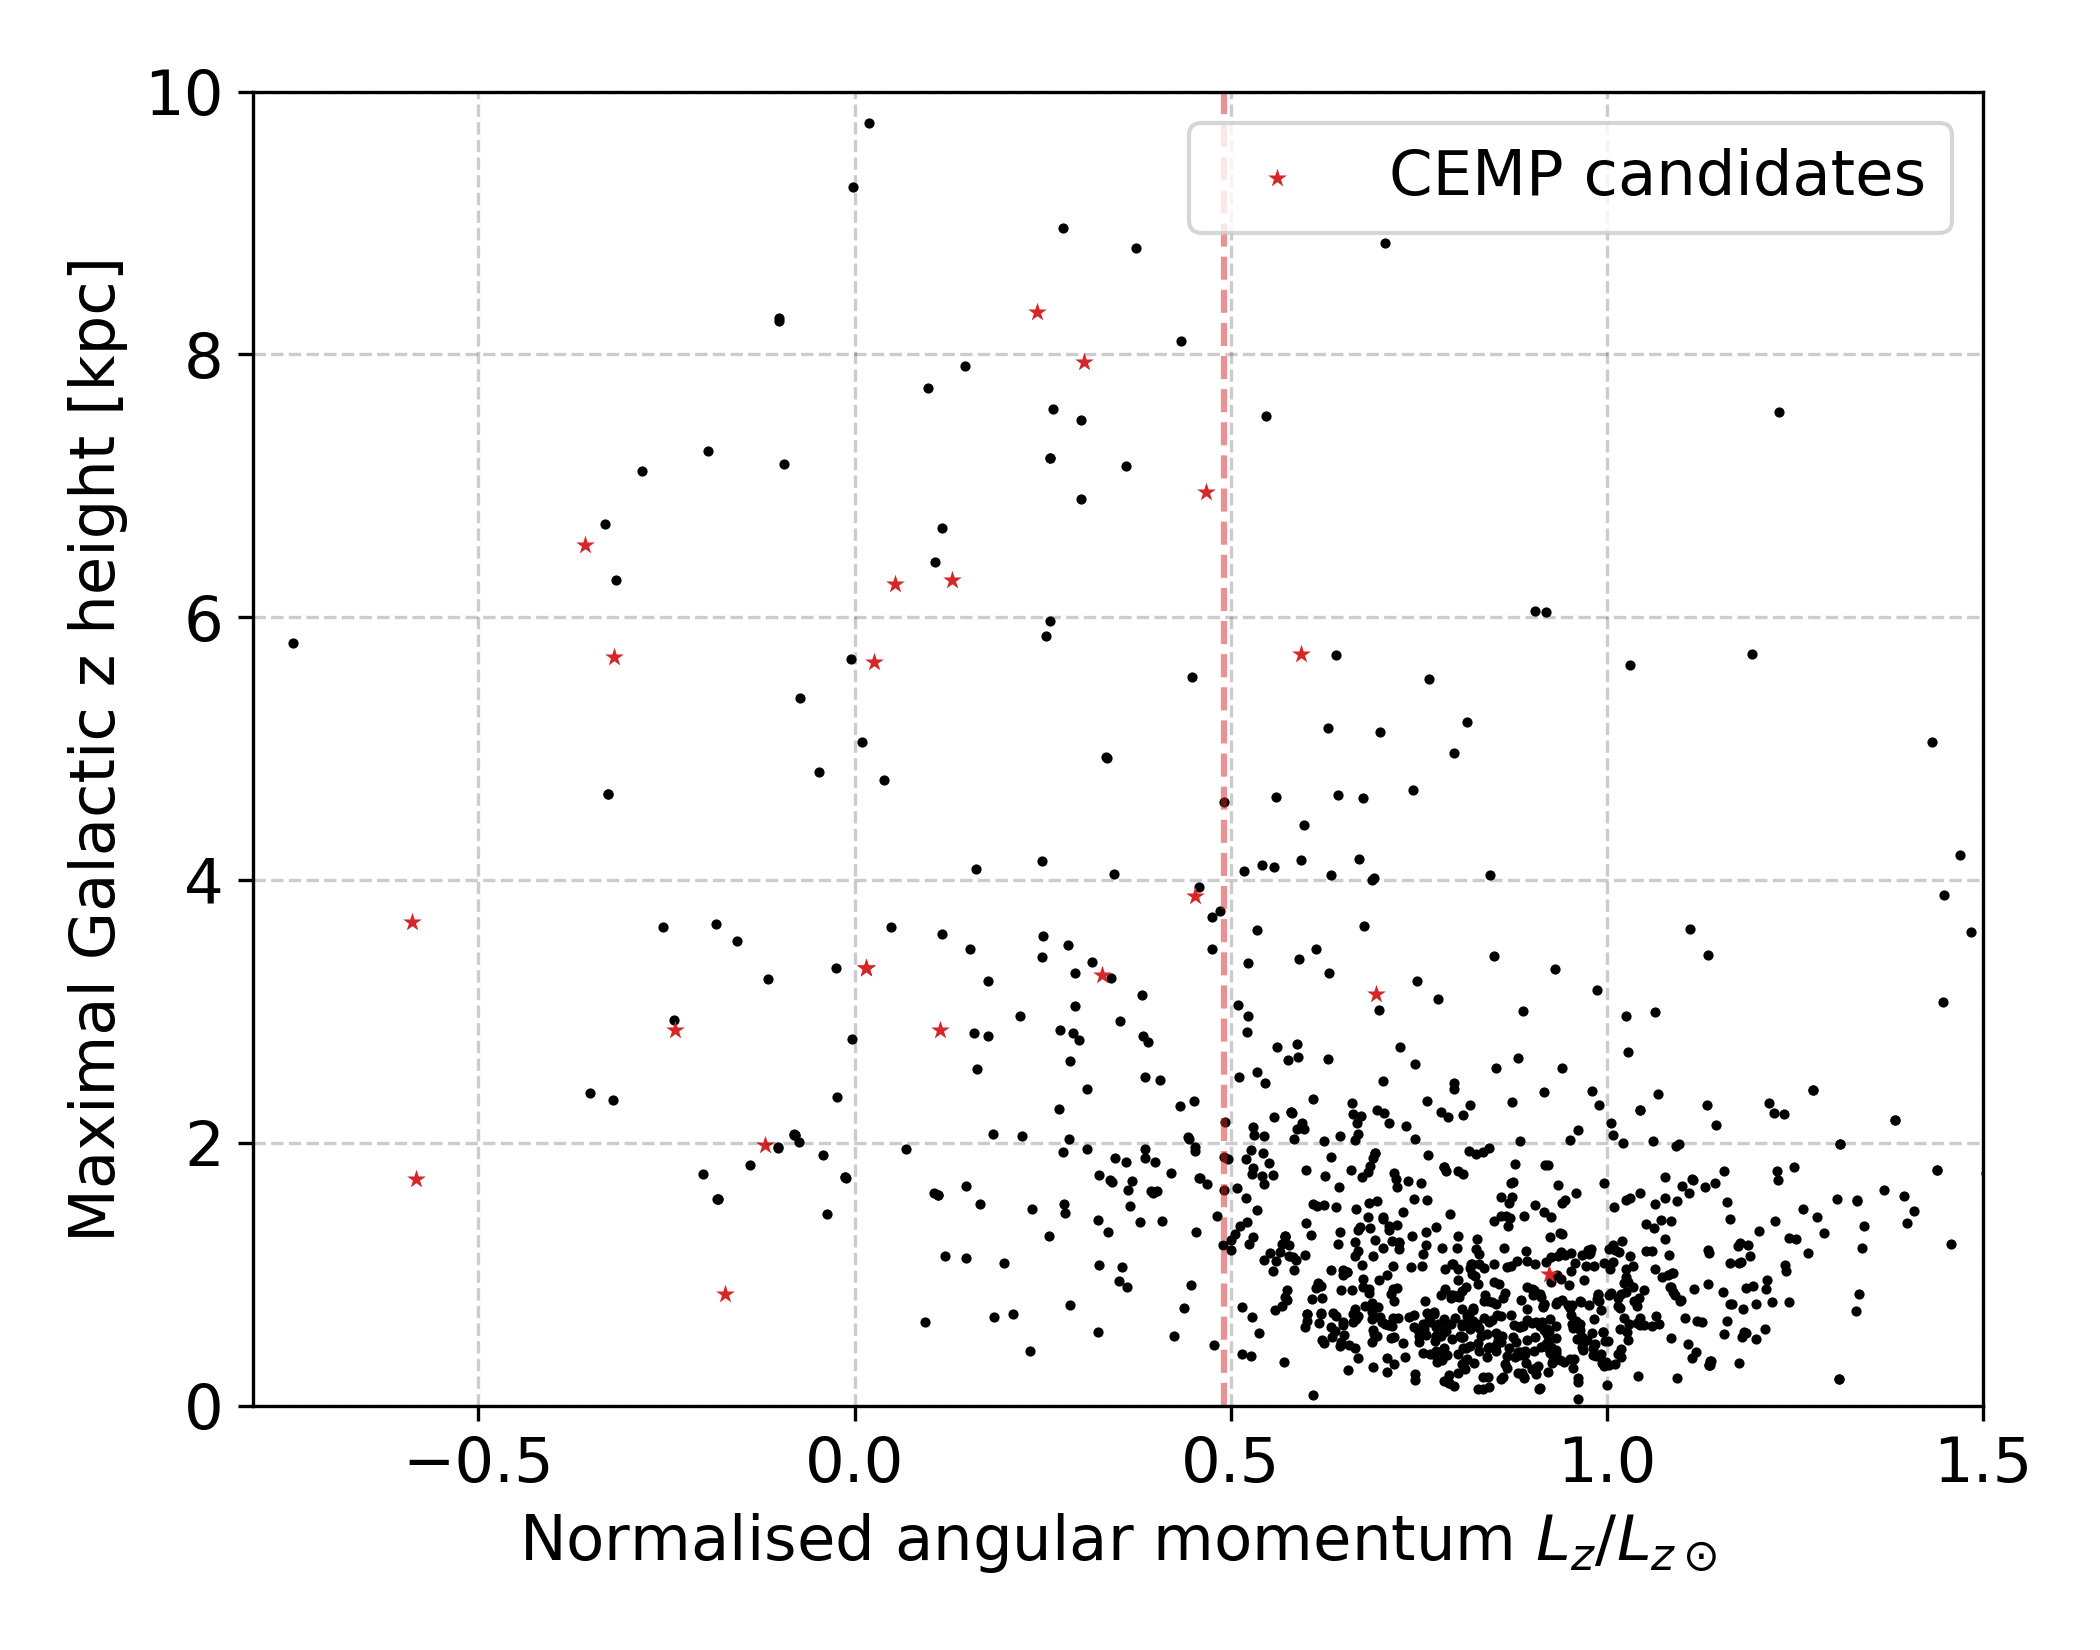
\includegraphics[width=0.6\textwidth]{carbon_orbits_zmax_lznorm.png}
	\caption{Distributions of maximal height above/below the Galactic plane reached by the detected stars on their orbit around the centre of the Galaxy. Heights are compared towards their normalised angular momentum L$_z$, where L$_odot$~=~$2033.6$~\kms~kpc. Vertical dashed line at L$_z$~=~$1000$~\kms~kpc highlights the transition from the halo to the disk population, where a majority of the halo stars is located below this threshold (the threshold was visually estimated from similar plots in \citet{2018ApJ...860L..11K}).  CEMP candidates are marked with star symbols.}
	\label{fig:orbits_zmax}
\end{figure}

\section{Follow-up observation}
\label{sec:asiago_cemp}

\begin{figure}
	\centering
	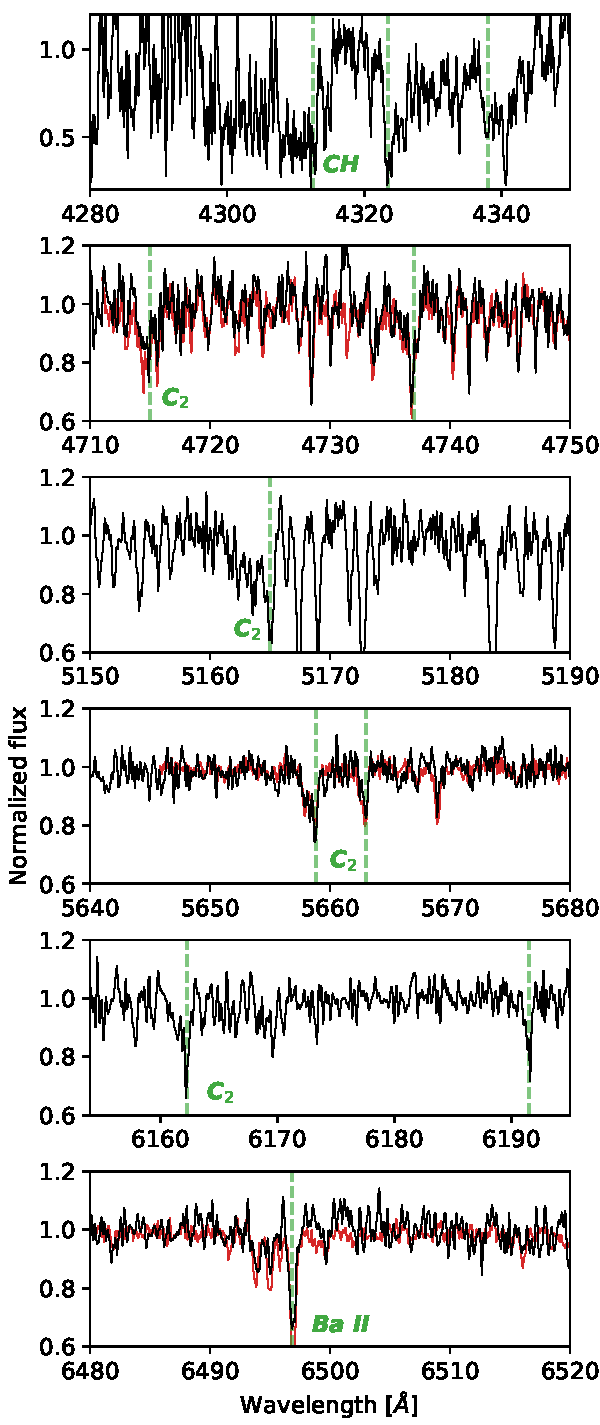
\includegraphics[width=0.55\textwidth]{asiago_cemp2.pdf}
	\caption{Subsets from the follow-up Asiago spectrum with resolving power comparable, but not identical, to the HERMES spectrum. It contains multiple spectral features used to evaluate carbon enhancement in a star and its carbon sub-class. Relevant spectral features (single line or tip of a molecular band) are marked with vertical dashed green lines and labels that represent a molecule or an element that is responsible for the features shown in the individual panel. The 2MASS identifier of the observed star is J11333341-0043060. In the wavelength ranges where it is available, the GALAH spectrum of the same star is shown in red.}
	\label{fig:asiago}
\end{figure}

To further classify and analyse one of the detected objects, a star with 2MASS identifier J11333341-0043060 was selected for a follow-up observation. We acquired its high-resolution Echelle spectrum (with the resolving power R $\sim 20,000$), using a spectrograph mounted on the $1.82$~m Copernico telescope located at Cima Ekar (Asiago, Italy). Because only a few of our detected candidates are observable from the Asiago observatory, we selected the best observable CEMP candidate, whose \Feh\ was determined by \TC\ to be $-0.96$. The selected star, with V = $12.79$, was on the dark limit of the used telescope, therefore low SNR was expected. The one-hour long exposure of the selected object was fully reduced, normalised order by order, and shifted to the rest frame.

Although the acquired spectrum covers a much wider and continuous spectral range (from 3900 to 7200~\AA) than the HERMES spectra, only subsets, relevant for the classification of carbon-enhanced stars are presented in Figure \ref{fig:asiago}. They were identified by visually matching our observed spectrum with the published moderate-resolution spectral atlas \cite{1996ApJS..105..419B} of peculiar carbon stars. Where available, the GALAH spectrum is shown alongside the Asiago spectrum. Carbon enhancement is not expected to vary over a period of several years, therefore both spectra should show similar features. The second and fourth panel in Figure \ref{fig:asiago} confirm that both observations indicate a similar degree of carbon enhancement.

Following the classification criteria of carbon stars, we determined that the star belongs to the C-H sub-class. The definitive features for this class are strong molecular CH bands, prominent secondary P-branch head near 4342~\AA\ (top panel in Figure \ref{fig:asiago}), and noticeable Ba II lines at 4554 and 6496~\AA\ \cite{2018ApJS..234...31L}, which are all present in the spectrum. The star definitely does not have a high ratio between $^{13}$C and $^{12}$C isotopes as the Swan features corresponding to $^{13}$C are clearly not present, therefore it can not be of a C-J sub-class.

Following the current state of knowledge \cite{1990ApJ...352..709M, 2016AA...586A.158J, 2016ApJ...826...85S} that most, if not all, C-H stars show clear evidence for binarity, we compared the radial velocity between both observations. They hint at the variability of the object as the follow-up radial velocity ($126.75 \pm 1.63$ \kms) deviates by more than $3$~\kms\ from the velocity ($123.43 \pm 0.08$ \kms) observed as part of the GALAH survey. The time span between the two observations is more than 2.5~years, where the exact JD of the observation is $2458090.702$ for the Asiago spectrum, and $2457122.095$ for the GALAH spectrum. Further observations along the variability period would be needed to confirm whether it is a multiple stellar system.

\section{Conclusions}
\label{sec:summary_cemp}
This work explores stellar spectra acquired by the HERMES spectrograph in order to discover peculiar carbon-enhanced stars, which were observed in the scope of multiple observing programmes conducted with the same spectrograph.

We show that the spectra of such stars are sufficiently different from other stellar types to be recognisable in high-resolution spectra with limited wavelength ranges. This can be done using a supervised procedure, where some knowledge about the effects of carbon enhancement on the observed spectra is put into the algorithm, or using an unsupervised method. The latter was used to identify observed stars solely on the basis of acquired spectra. By combining both methodologies we identified 918 unique stars with evident signs of carbon enhancement of which 12 were already reported in the literature. Out of all matched objects from the literature, we were unable to detect and confirm 16 ($57$~\%) CH and 15 ($93$~\%) CEMP stars with our procedures. As some of those objects were proven to contain carbon enhancement detectable outside the HERMES wavelength ranges, this would have to be taken into account to say more about the underlying population of carbon-enhanced stars. In addition to a detection bias imposed by the analysis of C$_2$ bands and exclusion of CN, and CH molecular bands that might be excitated in different temperature ranges, varying degree of carbon-enhancement also has to be accounted for accurate population studies. As shown by \citet{2016ApJ...833...20Y}, CEMP stars can be found within a wide range of absolute carbon abundances. When an object selection is performed with a pre-defined threshold, as in the case of our supervised methodology, this may reduce the number of objects in only one of the sub-classes. In the case of CEMP stars, this selection may influence a number CEMP-no stars that are known to have lower absolute carbon abundance \cite{2016ApJ...833...20Y}.

The identified objects were separated into dwarf and giant populations using their stellar atmospheric parameters that were also used to select possible CEMP candidates. All of the detections, with multiple observations at different epochs, were investigated for signs of variability. More than half of the repeats show signs of variability in their measured radial velocities. This could be an indicator that we are looking at a pulsating object or a multiple stellar system.

With a follow-up observation of one of the identified stars, we were able to confirm the existence of carbon-rich molecules in its atmosphere in a wider wavelength range. The acquired spectrum was also used to determine its sub-class. Variation in radial velocity points to a possible variable nature of the star or binarity that is common for C-H stars.

Follow-up observations are required to confirm variability of radial velocities observed for some of the detected carbon-enhanced stars and further investigate their nature. Careful spectral analysis, with the inclusion of carbon enhancement in models, is needed to confirm the metallicity levels of the metal-poor candidates. 

The list of detected stars presented in this chapter is accessible as electronic table through the CDS. Detailed structure is presented in Table \ref{tab:out_table}. The list also includes stars from the literature, matched with our observations, for which we were unable to confirm their carbon enhancement. The list could be used to plan further observations, allowing a better understanding of these objects.

\begin{figure}
	\centering
	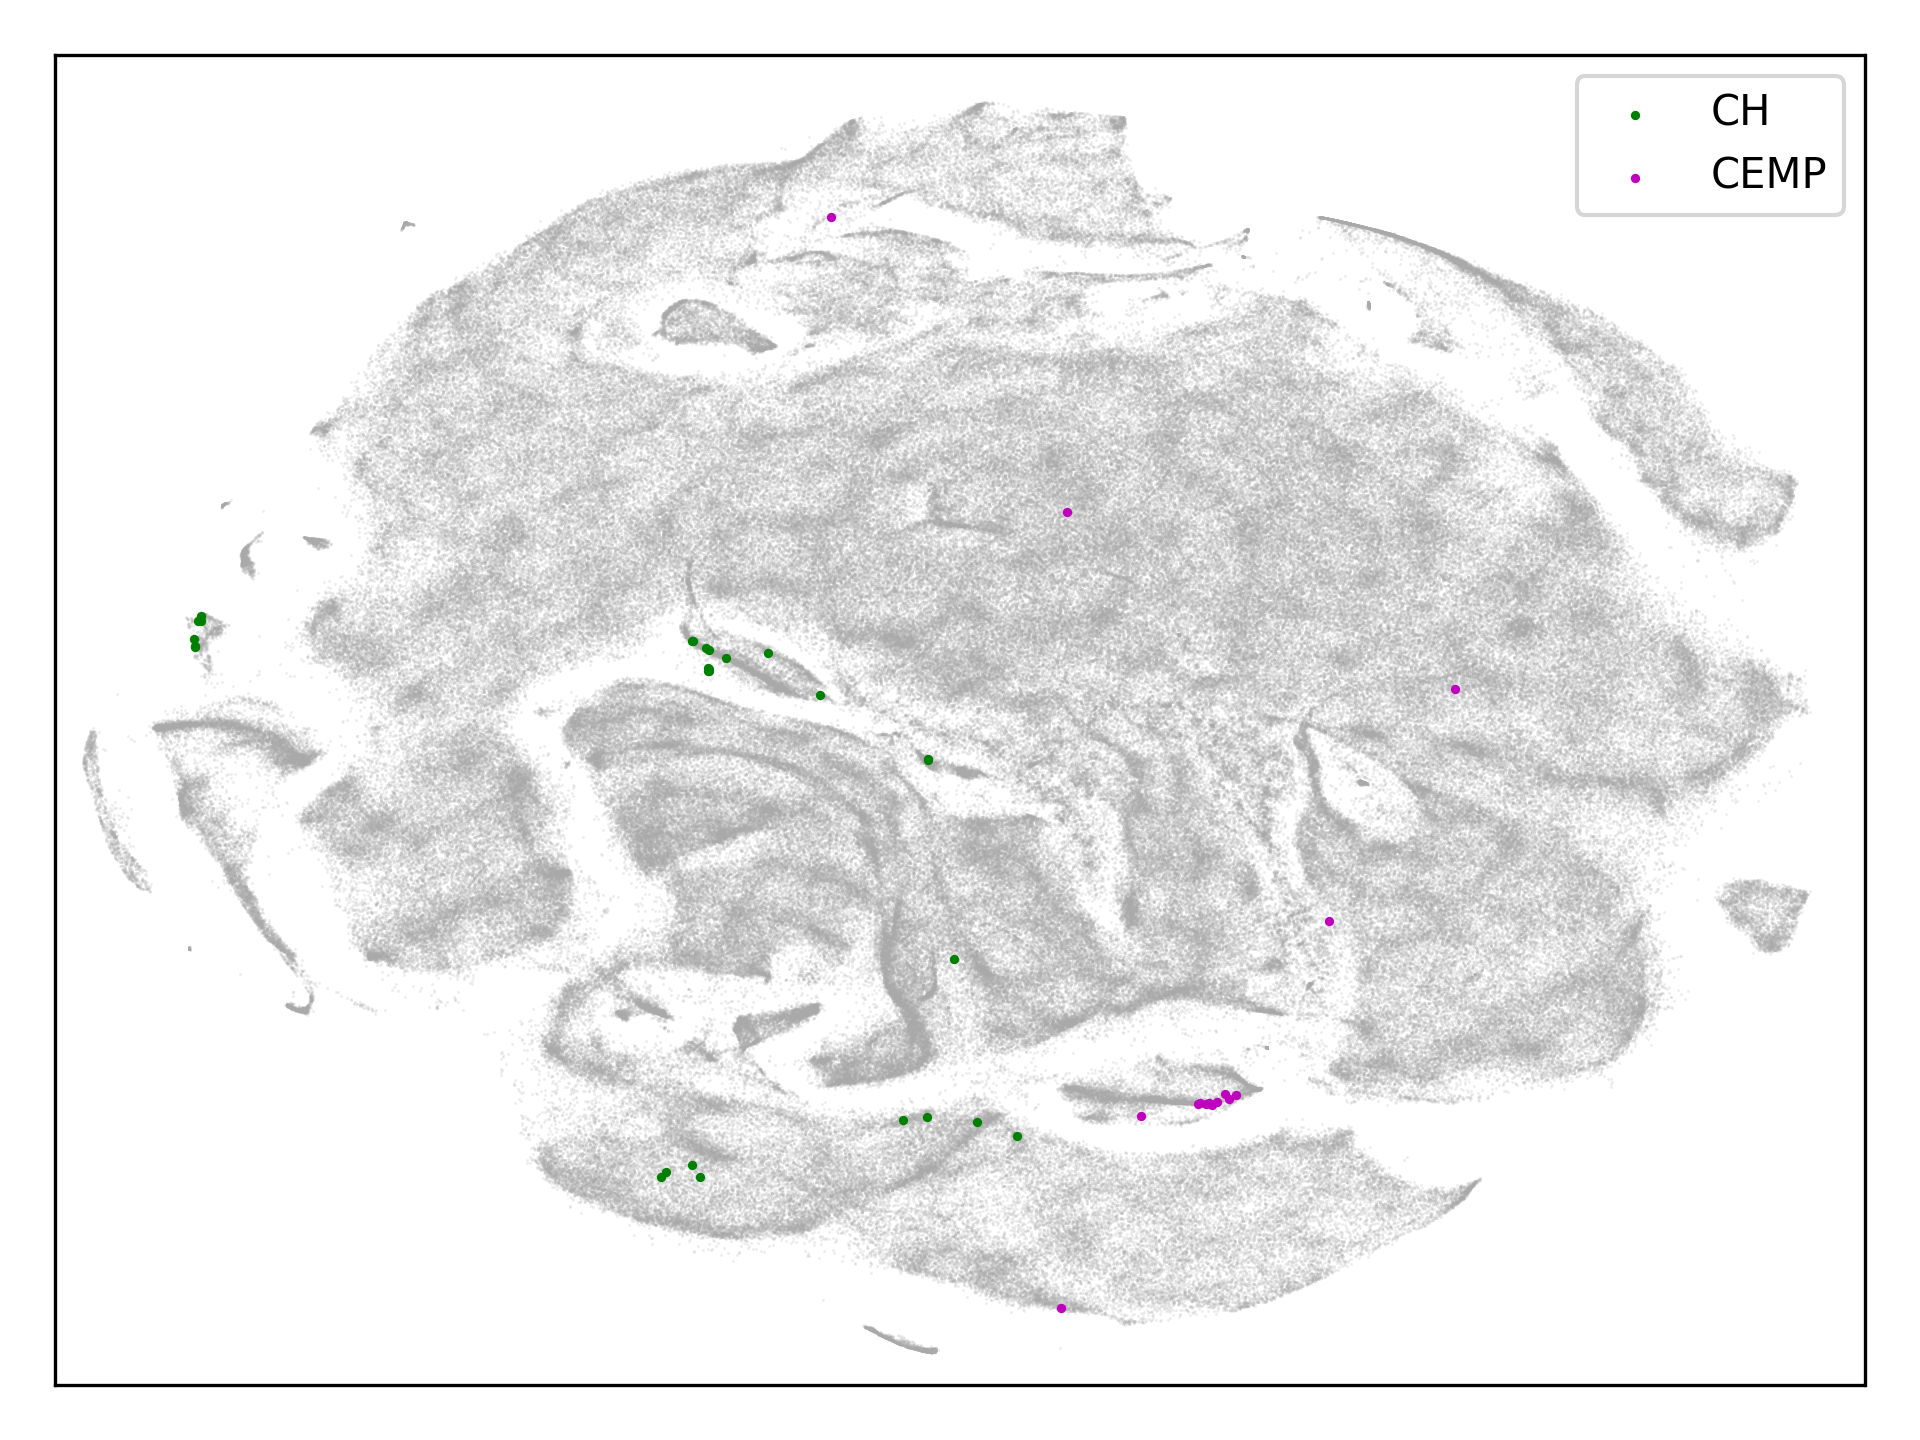
\includegraphics[width=\textwidth]{tsne_refpapers.png}
	\caption{t-SNE projection with marked known carbon-enhanced and CEMP objects from multiple different catalogues found in the literature that are also part of our analysed set of spectra. The dense clump of known CEMP stars is located close to our region of detected CEMP stars.}
	\label{fig:tsne_ref_ch}
\end{figure}

\begin{figure}
	\centering
	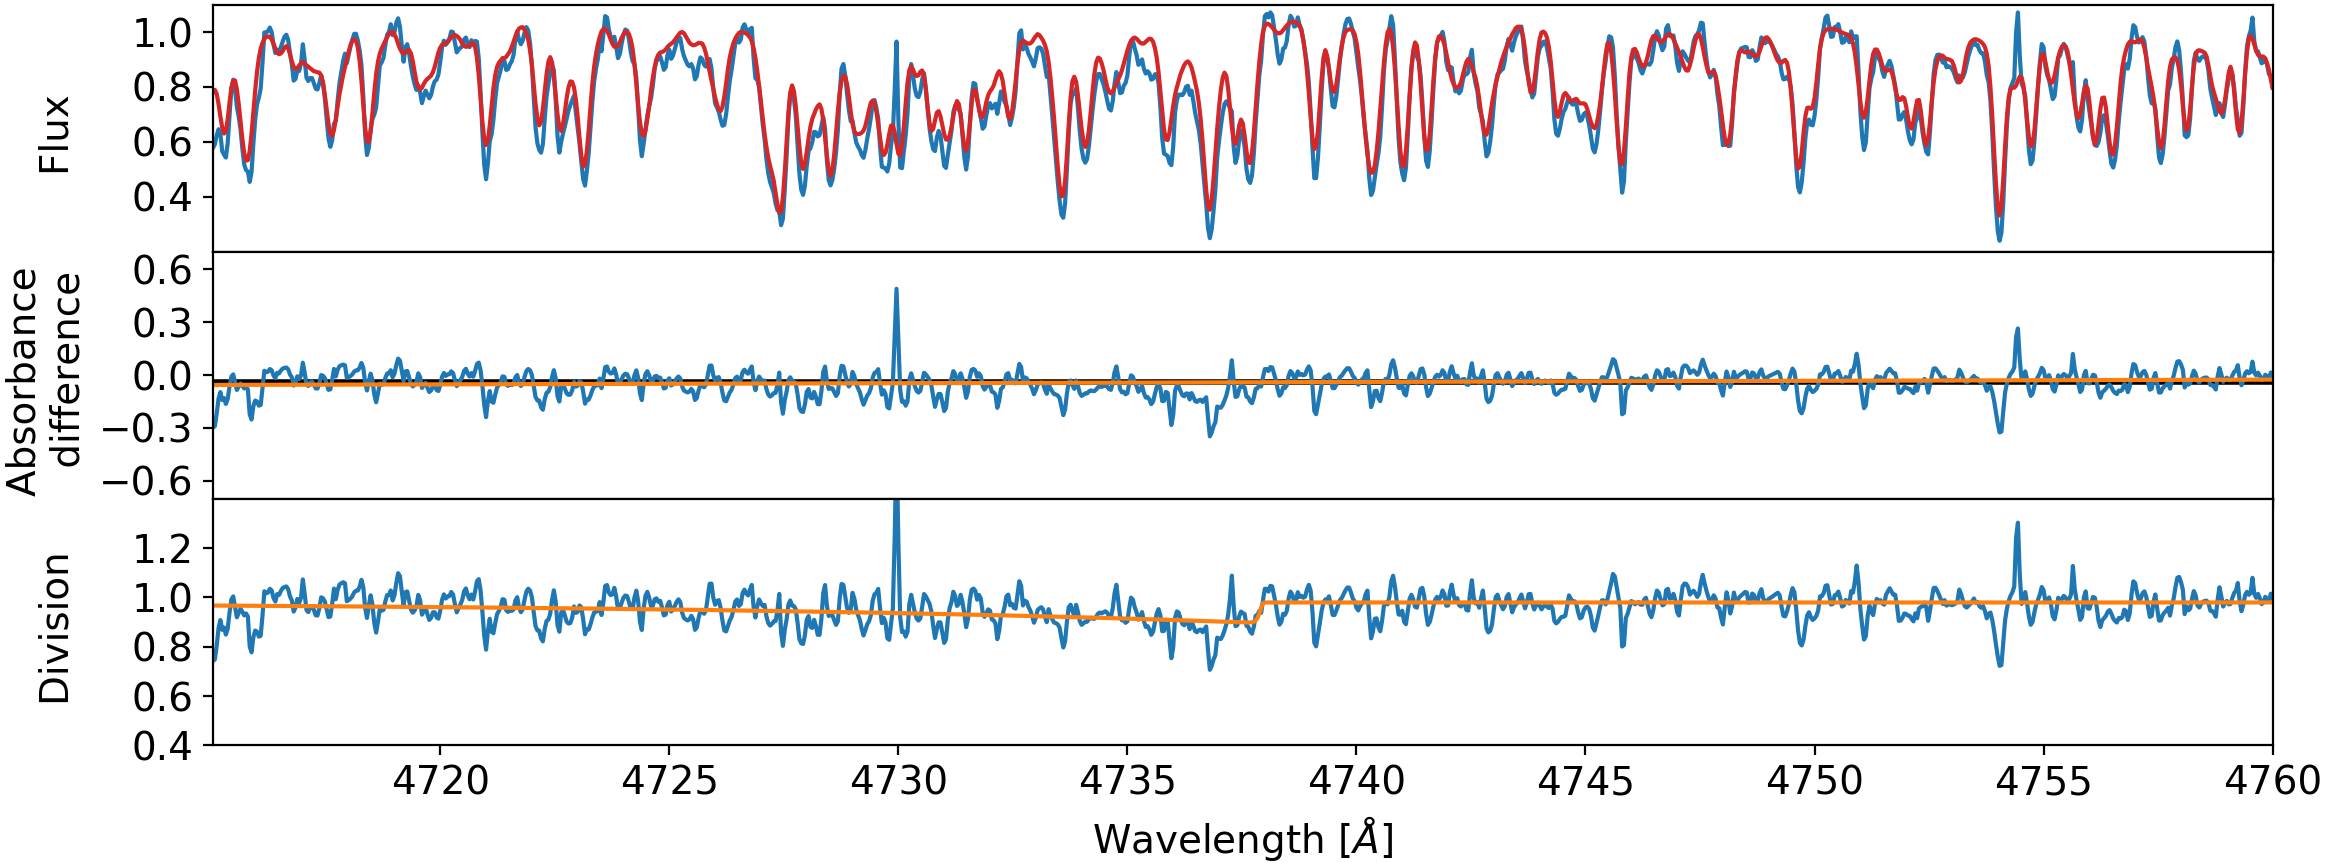
\includegraphics[width=\textwidth]{last_170515005101173.png}
	\caption{Equivalent plot as in the Figure \ref{fig:carbon_example} showing the last of 400 spectra, ordered by their degree of carbon enhancement, selected by the supervised methodology.}
	\label{fig:carbon_last_supervised}
\end{figure}

\begin{figure}
	\centering
	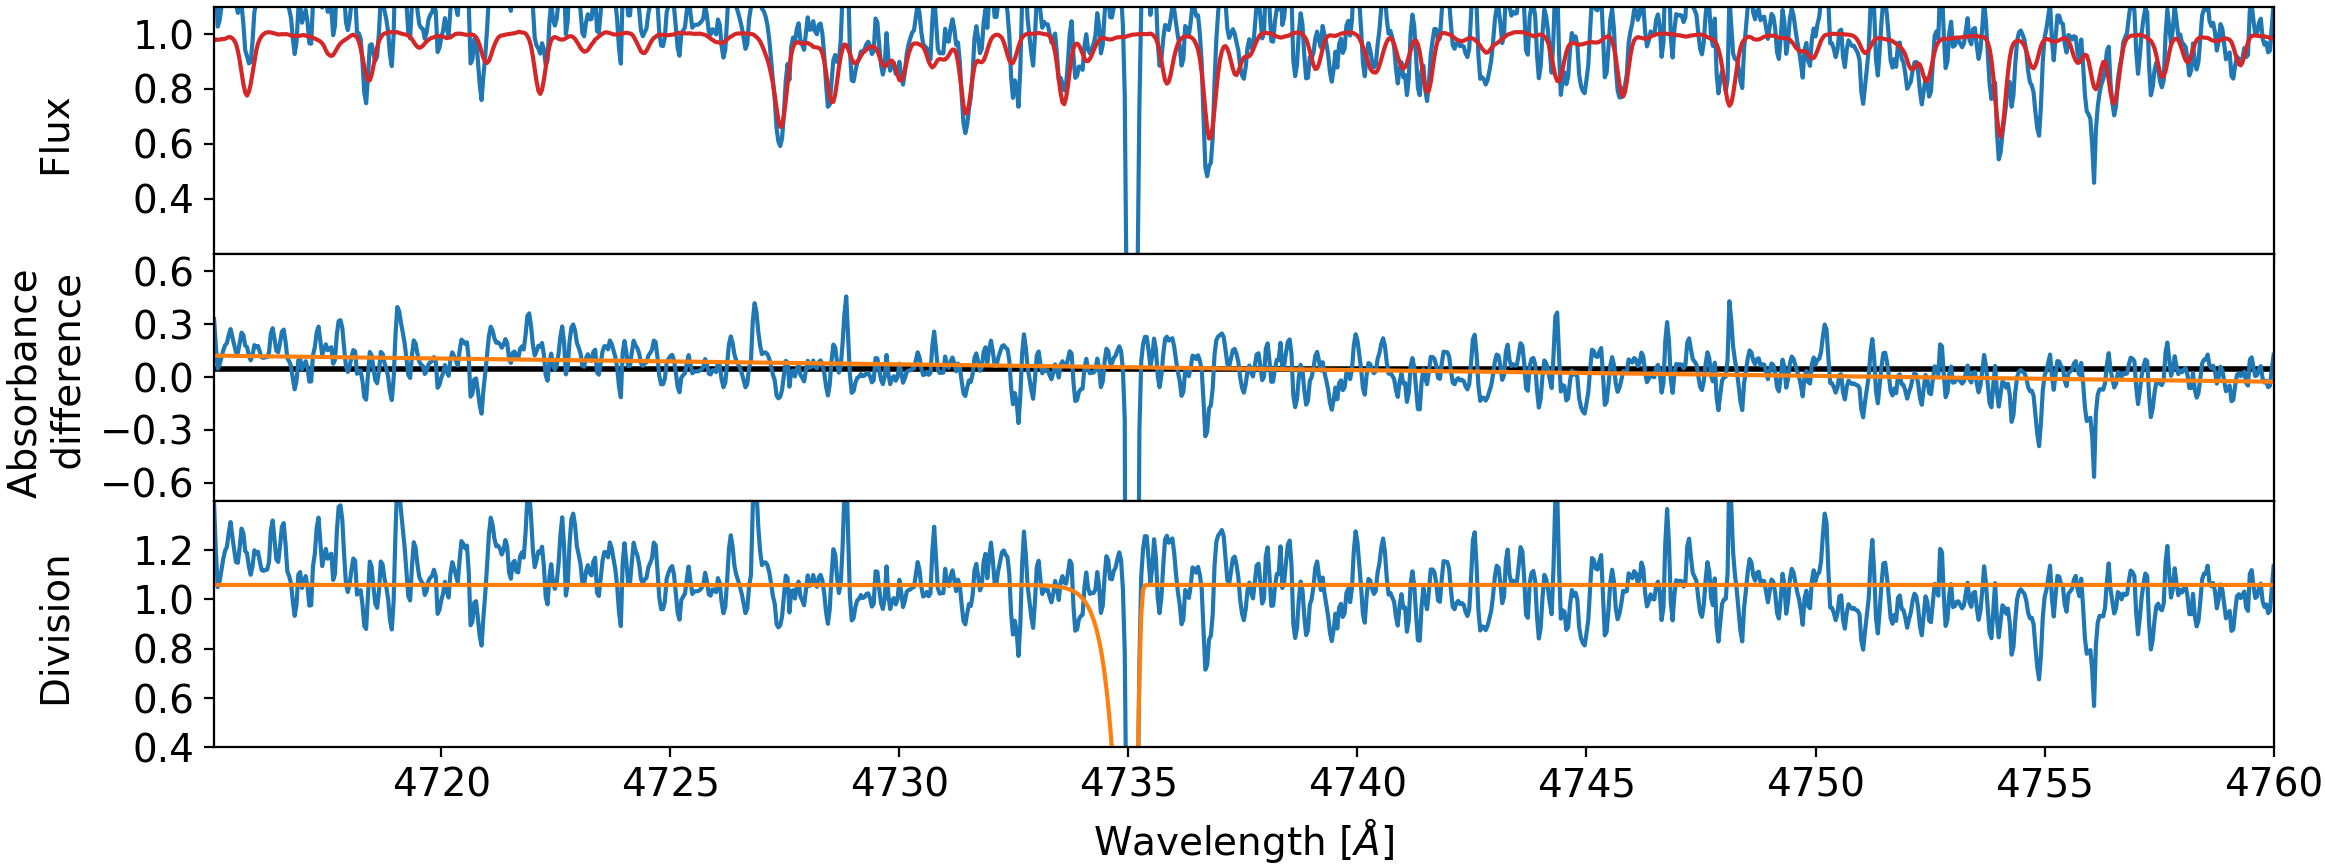
\includegraphics[width=\textwidth]{bad_fit1_150902002901051.png}
	\caption{Equivalent plot as in the Figure \ref{fig:carbon_example} but representing grossly over exaggerated carbon enhancement by a fit that describes a reduction problem (a cosmic ray in a subtracted sky spectrum).}
	\label{fig:bad_fit1}
\end{figure}

\begin{figure}
	\centering
	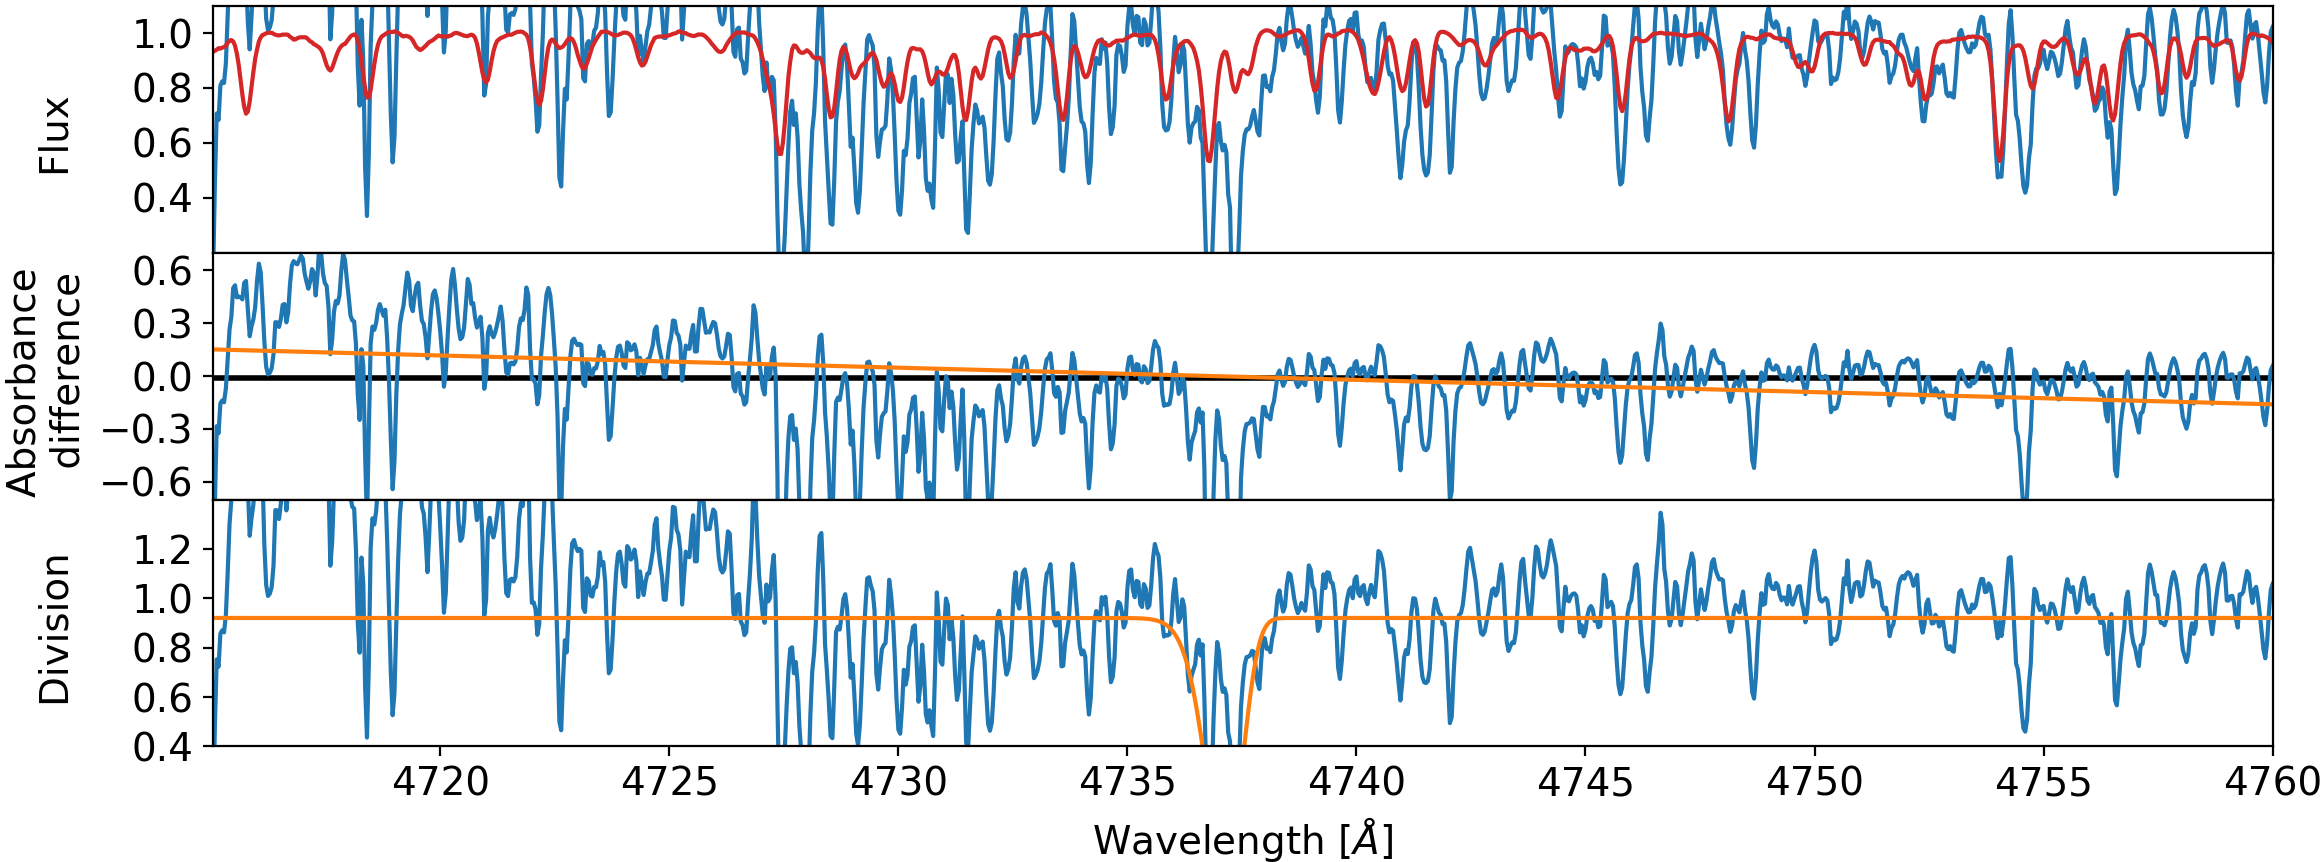
\includegraphics[width=\textwidth]{bad_fit2_150603001801056.png}
	\caption{Equivalent plot as in the Figure \ref{fig:carbon_example} but representing a fit to absorption lines of a double-lined spectroscopic binary. Final fit is not skewed as would be expected in the case of carbon enhancement.}
	\label{fig:bad_fit2}
\end{figure}


\chapter{Peculiar emission stars}
\label{chap:peculiars_emis}
This chapter has been adapted from the paper in preparation titled \textit{The GALAH survey: Characterization of emission-line stars with spectral modelling using autoencoders} \cite{2020arXiv200603062C} whose first author is author of this Doctoral thesis. The used computer code is published on GitHub platform \footnote{\url{https://github.com/kcotar/GALAH-suervey-Emission-lines-and-autoencoders}} and results of the analysis as a catalogue on the VizieR service \footnote{\href{http://vizier.u-strasbg.fr/viz-bin/}{exact link will be available after the paper is published}}.

Among all machine learning approaches, neural network structures are receiving the highest interest in all fields of big data analysis in recent years. Astronomy is no exception in this regard. In previous Chapter \ref{chap:peculiars_chem} we saw that peculiar stars are commonly detected by comparing observed spectra with reference spectra of stars that do not show any peculiarities in them. In this chapter we explore the autoencoder structure that provides us with the reference spectra for the comparison. Whenever we are interested in the precise elemental abundances (as used in Chapter \ref{chap:clusters}), the first step in their determination of stellar physical parameters that could be based on the strongest hydrogen Balmer lines in stellar spectra. As any deviations in their shape might endanger the analysis, we tried to identify all stars whose spectrum shows emission-lines in the Balmer region. The chapter begins with Section \ref{sec:intro_emis} that gives a detailed description of the problem and presents multiple scenarios of why and how emission-lines can be used and identified. In Section \ref{sec:det_chart} we explain our analysis pipeline whose main components are the generation of reference spectra (Section \ref{sec:ref_modeling}) and identification of multiple emission features (Sections \ref{sec:hahbemis} and \ref{sec:nebularemis}). The temporal variability of detected emissions is analysed in Section \ref{sec:temporal}. The results are summarised and discussed in Section \ref{sec:discussion_emis}.

\section{Introduction}
\label{sec:intro_emis}
The identification of peculiar stars, whose spectra contain emission lines, is of interest to a wide field of stellar research. Spectral complexity of such stars brings insight into the ongoing physical processes on and around the star. Presence of emission lines hints to an optically thin material that surrounds a star. Such optically thin structures can be present at different evolutionary stages of the star. As those stages are temporally short compared to the stellar life span, they are regarded as peculiar at that time.

Emission features in stellar spectra might adversely impacted the quality of stellar parameters and abundances determined by automatic data analysis pipelines that are only configured to produce the best results for most common stellar types. Examples of how these features might compromise spectroscopic measurements when we assume that a star is not peculiar include the determination of effective temperature \cite{2011A&A...531A..83C, 2018A&A...615A.139A, 2019A&A...624A..10G}, computation of stellar mass \cite{2016ApJ...823..114N, 2016A&A...594A.120B}, and the effects of self broadening on line wing formation \cite{2000A&A...363.1091B, 2008A&A...480..581A}. Highly accurate measurement of the hydrogen absorption profiles are needed in those cases. Any deviations in the line shapes from model predictions would produce misleading results. We would therefore like to know if the investigated line is modified by additional, unmodelled physical process or spectral reduction process.

Stars with evident emission lines populate a wide variety of regions on the HR diagram. Because of possible overlaps between different stellar types, detailed photometric (especially in the infrared region where warm circumstellar dust disc can be identified) and spectroscopic observations are needed for an accurate physical explanation of the observed features. An examples of such work is presented in \citet{2019MNRAS.488.5536M}, who performed detailed a multi-band photometric study of an emission-line star, originally discovered on objective prism plates. The detailed photometric time-series study described in that work, together with observations of the star's infrared excess, led to the star VES~263 being identified as a massive pre-main-sequence star and not a semi-regular AGB cool giant as classified previously. In a similar way, \citet{2020arXiv200207852L} performed an analysis of the stellar object V* CN Cha, which had previously been identified as an emission star. By studying a long photometric time-series of the star, they concluded that the object was most likely a symbiotic binary star system whose emission was lined to a long-duration, low-luminosity nova phase.

Numerous different physical processes that can contribute to the complex shapes of the H$\alpha$ emission profile are discussed by \citet{1996A&AS..120..229R, 2011AJ....141..150J, 2014ApJ...795...82S, 2018AJ....156...97I}, who compare observations with expected physical models. Following the classification scheme introduced by \citet{2007ASSL..342.....K}, emission-line stars are predominately observed in close binaries, earliest-type, latest-type, and pre-main sequence stars. For systems in which mass accretion is occurring, the examination of emission lines can allow the mass accretion rate onto the central star to be estimated \cite{2003ApJ...582.1109W, 2004A&A...424..603N}. The procedure involves measuring simple indices (such as the equivalent width and broadening velocity) of the emission lines in the stars's spectrum.

In recent years, multiple dedicated photometric and spectroscopic surveys (e.g. \cite{2008MNRAS.384.1277W, 2008MNRAS.388.1879M, 2012ApJS..200...14M, 2012AJ....143...61N, 2014MNRAS.440.2036D, 2016MNRAS.456.1424A, 2016ASPC..505...66N}), and exploratory spectral classifications of large unbiased all-sky spectroscopic observational datasets (e.g. \cite{1999A&AS..134..255K, 2012MNRAS.425..355R, 2015A&A...581A..52T, 2016ASPC..505...66N, 2016RAA....16..138H, 2017ApJS..228...24T}) have been performed, each finding from hundreds to tens of thousands of interesting emission-line stars. Some of these surveys provide a basic physical classification in addition to an emission detection. Therefore they can be used as source lists for further in-depth studies of individual stars.

If a star is engulfed in a hot rarefied interstellar medium or stellar envelope, emission features of the forbidden lines (the most commonly studied of which are the [NII] and [SII] lines) could be observed in its spectrum, providing an insight into the temperature, density, intrinsic movement, and structure of its surrounding interstellar environment \cite{1973ApJ...184...93B, 1993Ap&SS.204..205R, 2005MNRAS.361..813E, 2016A&A...591A..74D, 2017A&A...604A.135D}.

Focusing on spectroscopic data, procedures for the detection of emission lines can roughly be separated into two categories. Simpler procedures searching for obvious emitters above the global continuum \cite{2015A&A...581A..52T, 2016ASPC..505...66N, 2016RAA....16..138H, 2016ASPC..505...66N} and more complex procedures, where the observed spectrum is compared to an expected stellar spectrum of a normal star \cite{2013ApJ...776..127Z}. The reference spectra in the latter case can be generated using exact physics-based stellar modelling or data-driven approaches. Of these, the data-driven approaches can be separated into supervised and unsupervised generative models, where, for the later, it is not required to provide an estimate of the stellar parameters for a given spectrum in advance. To predict a reliable model using supervised models, we must determine the correct stellar labels of an emission star in advance. This can pose a serious limitation if the strongest lines in the acquired spectrum can be populated by an emission feature, which happens for \G\ and RAVE spectra \cite{2013ApJ...776..127Z}. In light of the future publication of Gaia RVS spectra as part of Gaia DR3 for several million of stars, it is thus important to develop tools to identify emission-line stars, as we aim to do in this study via GALAH spectra.
% kak odstavek: poudariš da boš tukaj delal to for in zakaj so autoencoderji kul, recimo

\section{Detection and characterization}
\label{sec:det_chart}
The first attempts to discover H$\alpha$/H$\beta$ emission spectra in GALAH survey observations were performed by \citet{2017ApJS..228...24T}, who also detected emission line stars in the Gaia-ESO \cite{2012Msngr.147...25G} dataset using the Gaussian fitting and arbitrary thresholding \cite{2015A&A...581A..52T}. \citet{2017ApJS..228...24T} used the unsupervised dimensionality reduction technique t-SNE \cite{2013arXiv1301.3342V} to group morphologically similar spectra. As the amplitude and shape of the observed emission can vary substantially depending on the astrophysical source, \citet{2017ApJS..228...24T} presumably detected only a portion of the strongest emitters. One of the reasons for this is the manual classification of data clumps determined by the clustering algorithm. In the case of weak emissions in an investigated clump (performed manually by the operator), an expressed emission feature must be strong enough to be visually perceived when looking at a spectrum. To broaden the range of detectability to include spectra with marginal levels of emission as well, a more sophisticated and partially supervised procedure must be employed.

To expand the search, our methodology uses additional prior knowledge about the expected wavelength locations of interesting emission spectral lines. The prior wavelengths are used to narrow down the interesting wavelength regions during the comparison between the spectrum of a possibly peculiar star and an expected (reference) spectrum of a star with similar physical parameters and composition.

\subsection{Spectral modelling using autoencoders}
\label{sec:ref_modeling}
A reference or a synthetic spectrum of a normal star without emission lines can be produced by a multitude of physics-based computational stellar models \cite{1993sssp.book.....K, 2005A&A...442.1127M, 2012ASInC...6...53D} or supervised generative data-driven approaches \cite{2015AAS...22530207N, 2019ApJ...879...69T}, whose common weakness is the need for prior knowledge of at least an approximate stellar parameters of an analysed stars used by the data-driven algorithm.

As some of our spectra do not have determined stellar parameters or they are flagged with warning signs that indicate different reduction and analysis problems (missing infrared arm, various reduction issues, bad astrometric solutions, \SME\ did not converge etc.), we focused on an unsupervised spectral modelling to produce our set of reference spectra. Given the large size of available training data set, we chose to use an autoencoder type of an artificial neural network (ANN) that is rarely used to analyse astronomical data. Its current use ranges from data denoising \cite{2017ChA&A..41..282Q, 2019arXiv190303105S, 2019MNRAS.485.2628L} to unsupervised feature extraction and feature based classification \cite{2015MNRAS.452..158Y, 2017RAA....17...36L, 2017ChA&A..41..318P, 2018arXiv180901434K, 2019arXiv191104320C, 2019ApJS..240...34M, 2019PASP..131j8011R}.

An autoencoder is a special kind of ANN, shaped like an hourglass, that takes input data (a stellar spectrum in our case), reduces it to a selected number of latent features (a procedure known as encoding) and tries to recover the original data from the extracted latent features (decoding process). Our dense, fully connected autoencoder consists of the data input layer, four encoding layers, a middle feature layer, four decoding layers and the output layer. The number of nodes (or latent spectral features) in the encoding part slowly decreases in the following arbitrary selected order: $75\%$, $50\%$, $25\%$, and $10\%$ of input spectral wavelength samples (4500 in the case of the red spectral arm). The exact numbers of nodes at each layer are shown in Figure \ref{fig:autoann}. At the middle feature layer, the autoencoder structure reduces to only $5$ relevant extracted features. Selecting a higher number of extracted features would also mean that the ANN structure could extract more uncommon spectral peculiarities which is not what we want. In our case, the goal is the reconstruction of a normal non-peculiar spectrum by extraction of a few relevant spectral features. Additionally, because of the low number of extracted features, our decoded output spectrum is a smoothed and denoised version of an input spectrum.

\begin{figure}
	\centering
	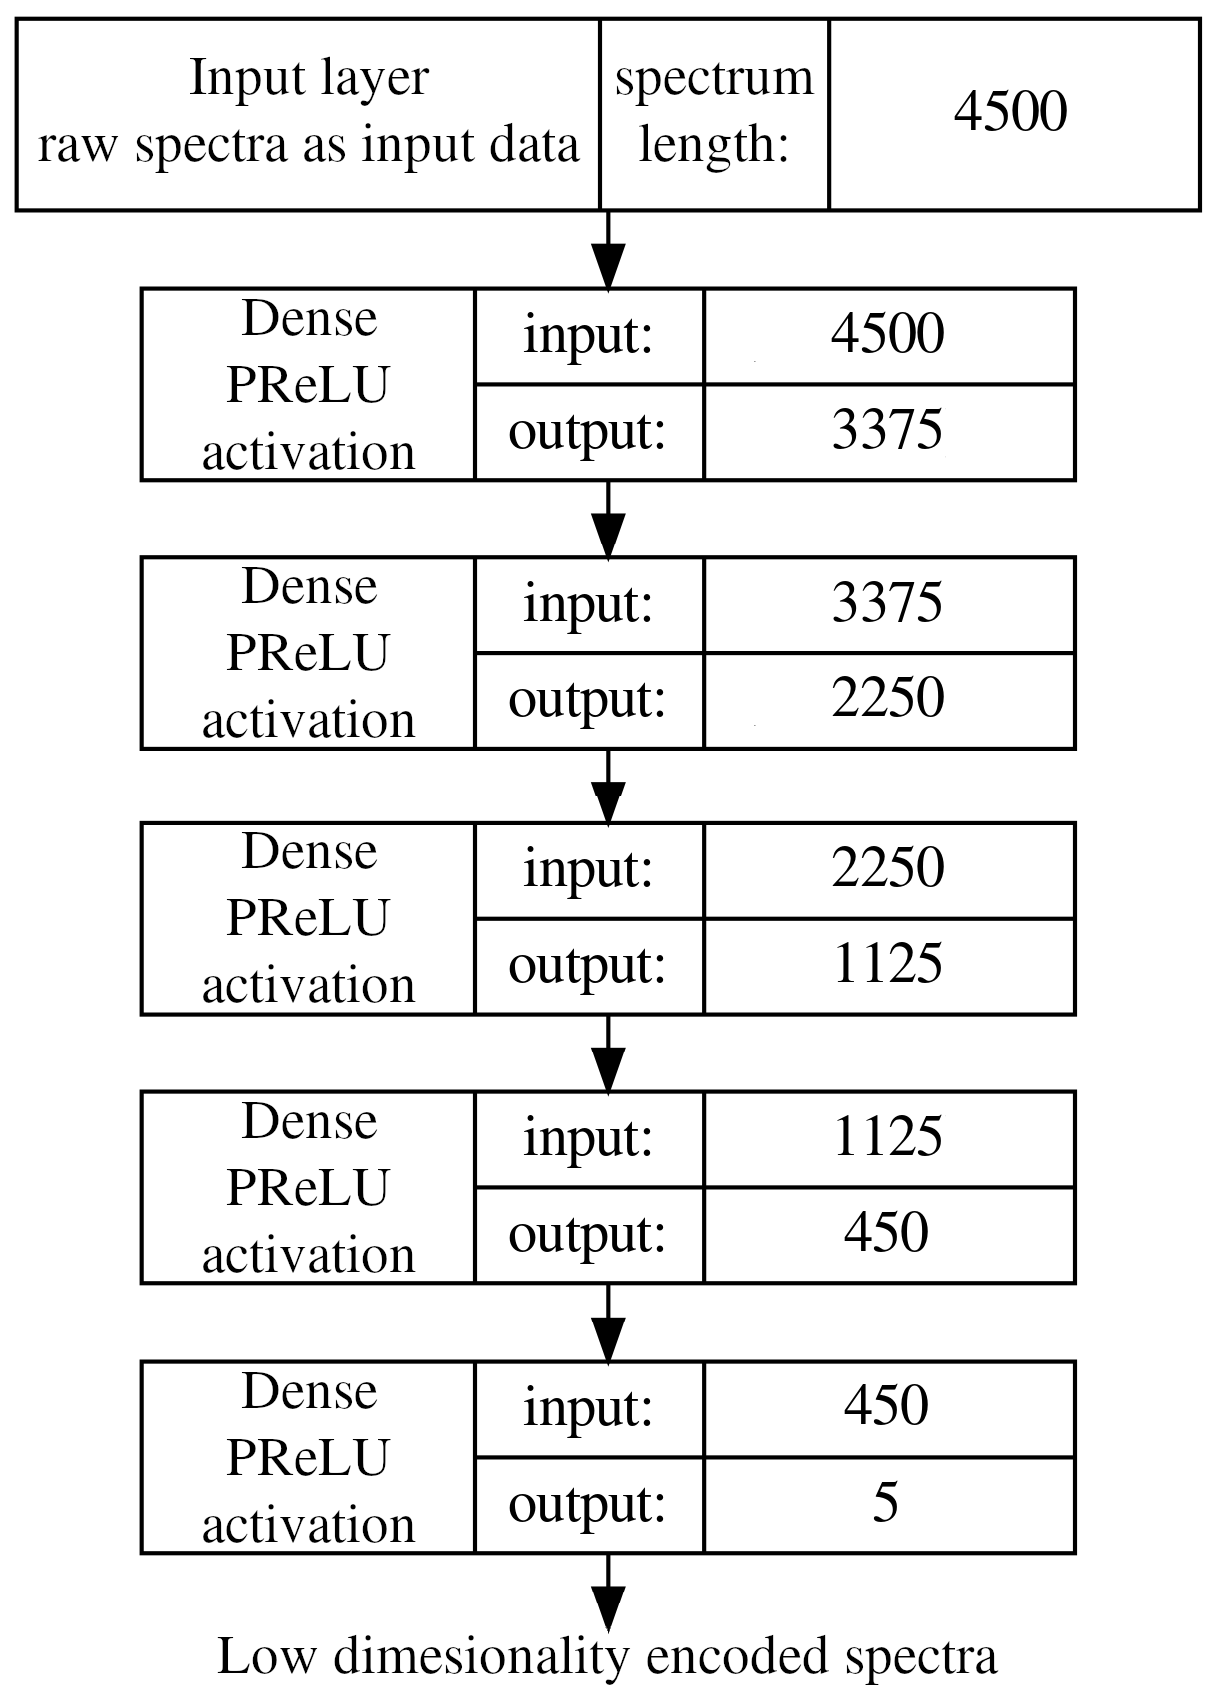
\includegraphics[width=0.6\textwidth]{ann_network_structure_a.png}
	\caption{Visual representation of an encoder part of the used autoencoder structure for the red spectral arm. After the input spectra are encoded, they are passed through the same inverted architecture to produce modeled low-noise spectra. The value in the right most column indicates a number of input and output connections to neighboring layers. The number of nodes in a layer is equal to the output value. The input spectrum length is given as the number of wavelength bins in a spectrum.}
	\label{fig:autoann}
\end{figure}

A visual representation of the described architecture is shown in Figure \ref{fig:autoann}. The shape of the decoding structure of the autoencoder is the same, except in a reverse order. The Parametric Rectified Linear Unit (PReLU, \cite{2015arXiv150201852H}) activation function defined as
\begin{equation}
f(x) = \begin{cases}
x, & \mathrm{if} x > 0 \\
ax, & \mathrm{if} x \le 0
\end{cases}
\label{equ:prleu}
\end{equation}
is used for all nodes of the network, with the exception of the final output layer that uses a linear (i.e. identity) activation function. The $x$ denotes one spectrum flux value in the first layer and one latent feature in the remaining layers. The free parameter $a$ in Equation \ref{equ:prleu} is optimised during the training phase.

If the network learns a physics-based generative model of a stellar spectrum, information contained in the extracted features should be related to real physical parameters, such as \Teff, \Logg, \Feh, and \vsin, or their mathematical combinations. 

To train our autoencoder, we created a set of presumably normal spectra (with no emission features), resampled to a common wavelength grid ($\delta \lambda$ equal to $0.04$ and $0.06$~\AA\ for the blue and red arm). Coverage of the grid is slightly wider than the range of an individual HERMES arm to account for variations in wavelength span because of stellar radial velocity and field curvature which slightly shifts wavelength span of every fiber on a CCD. Observations that did not completely fill the selected range were padded with continuum value of 1. To be classified as normal, spectra must suffice the following selection rules: signal to noise ratio (SNR) in the green arm must be greater than $30$, a spectrum must not contain any known reduction issues (\texttt{red\_flag}~=~0 in \citet{2017MNRAS.464.1259K}) and have valid spectral parameters (\texttt{flag\_sp}~<~16 in \citet{buder2020}). Although choosing \texttt{flag\_sp}~=~0 returns the spectra with the most trustworthy parameters, we choose to use this higher cutoff in \texttt{flag\_sp} to filter out only the strangest spectra and not to produce a set of spectra with well defined parameters. Spectra with 0~<~\texttt{flag\_sp}~<~16 include objects with bad astrometric solution, unreliable broadening, and low SNR that are still useful for our training process. From \citet{2017ApJS..228...24T, buder2018} and \citet{2019MNRAS.483.3196C}, we know that some GALAH spectra display peculiar chemical composition or consist of multiple stellar components. Therefore we removed all identified classes of peculiar spectra with the exception of stars classified as hot or cold that are actually treated as normal spectra in our case. Even such a rigorous filtering approach can miss some strange spectra.

After we applied these quality cuts, we were left with $482,900$ spectra, of which last $10\%$ were used as an independent validation set during the training process. Before the training, normalised spectra were inverted ($1$~$-$~normalised flux), which sets the continuum level to a value of $0$. The inversion improved the model stability and decreased the required number of training epochs.

The described autoencoder was trained with the Adam optimisation algorithm \cite{2014arXiv1412.6980K} for $350$ epochs. At every epoch all training spectra were divided into multiple batches of $40,000$ spectra, whose content is randomised at every epoch. A batch is a subset of data that is independently used during a training process. Such splitting and randomisation of training spectra into batches decreases the probability of model over-fitting. To enable the selection of the best network model, it was saved after the end of every training epoch. 

The loss score minimised by the Adam optimiser, shown in Figure \ref{fig:trainann}, was computed as a mean absolute error (MAE) between the input observed and decoded spectra defined as:
\begin{equation}
\label{equ_mae}
loss_\mathrm{MAE} = \frac{1}{N n_\lambda} \sum_{n=1}^{N}\sum_{i=1}^{n_\lambda}\left|f_{\mathrm{ae}, n, i} - f_{\mathrm{obs}, n, i}\right|,
\end{equation}
where N is the number of all spectra, $n_\lambda$ the number of wavelength bins in each spectrum,  $f_{\mathrm{ae}, n, i}$ the flux value of a decoded spectrum at one of the training epochs, and $f_{\mathrm{obs}, n, i}$ the flux value of a normalised observed spectrum. Such a loss function gives lower weight to gross outliers in comparison to the mean squared error (MSE). At the same time, outputs are closer to a median spectrum of spectra with a similar appearance and less affected by remaining peculiar spectra in the training set. 

\begin{figure}
	\centering
	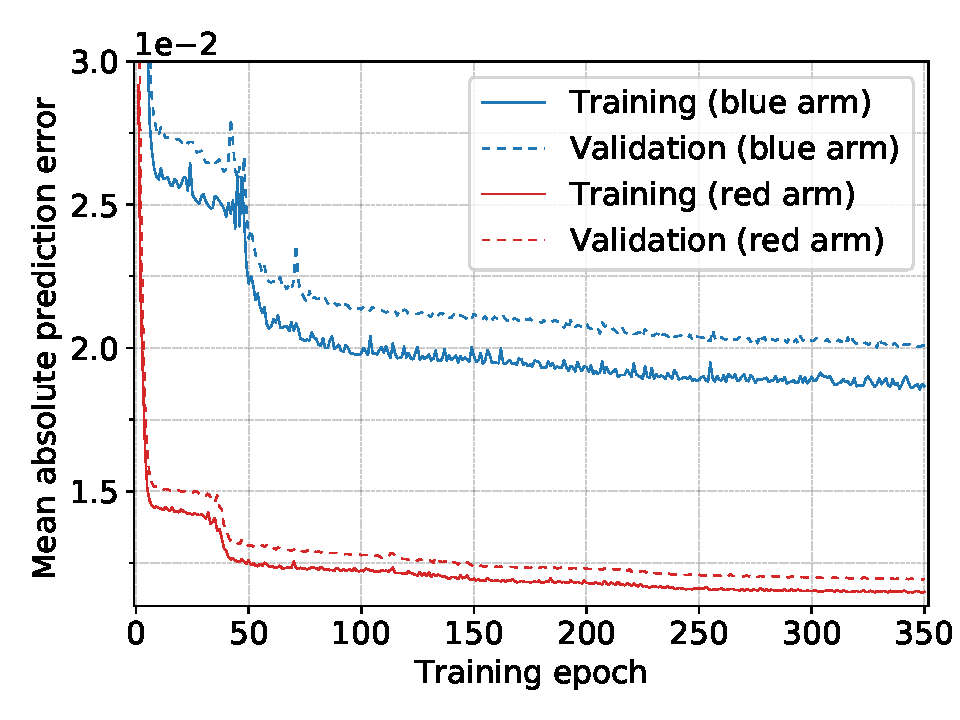
\includegraphics[width=0.6\textwidth]{ann_network_loss_ccd13.pdf}
	\caption{Prediction accuracy of the blue and red arm autoencoders at different training epochs. The prediction error is computed as a sum of all absolute differences between the input and output data set (see Equation \ref{equ_mae}). Shown are training (solid line) and validation curves (dashed line) which do not show any strong model over-fitting on the training set. The curves indicate that both autoencoders learned in a similar way because the same optimiser was used. The blue arm model has a bit higher loss and shows slower learning because of a greater spectral complexity and lower signal to noise ratio in that wavelength region.}
	\label{fig:trainann}
\end{figure}

After examining the decoded outputs at different epochs in comparison with known normal and peculiar spectra, we decided to use the model produced after $150$ training epochs. After that, overall improvements of the model are minor, which increases the model opportunity to over-fit on a low number of peculiar spectra. After closer inspection of the last epoch, we found indications of over-fitting on known emission stars, which further confirms the validity of choosing a model with shorter training period (with greater prediction loss) and rejects the need for a longer model training.

To decrease the complexity of a dense neural network and reduce the required training time, two independent autoencoders were trained, separately for the blue and red HERMES spectral arms.

After the training and model selection were completed, all available $669,845$ spectra were run through the same autoencoder to produce their high SNR reference spectra. An example of four such spectra is shown in Figures \ref{fig:refann} and \ref{fig:refann2}.

\begin{figure}
	\centering
	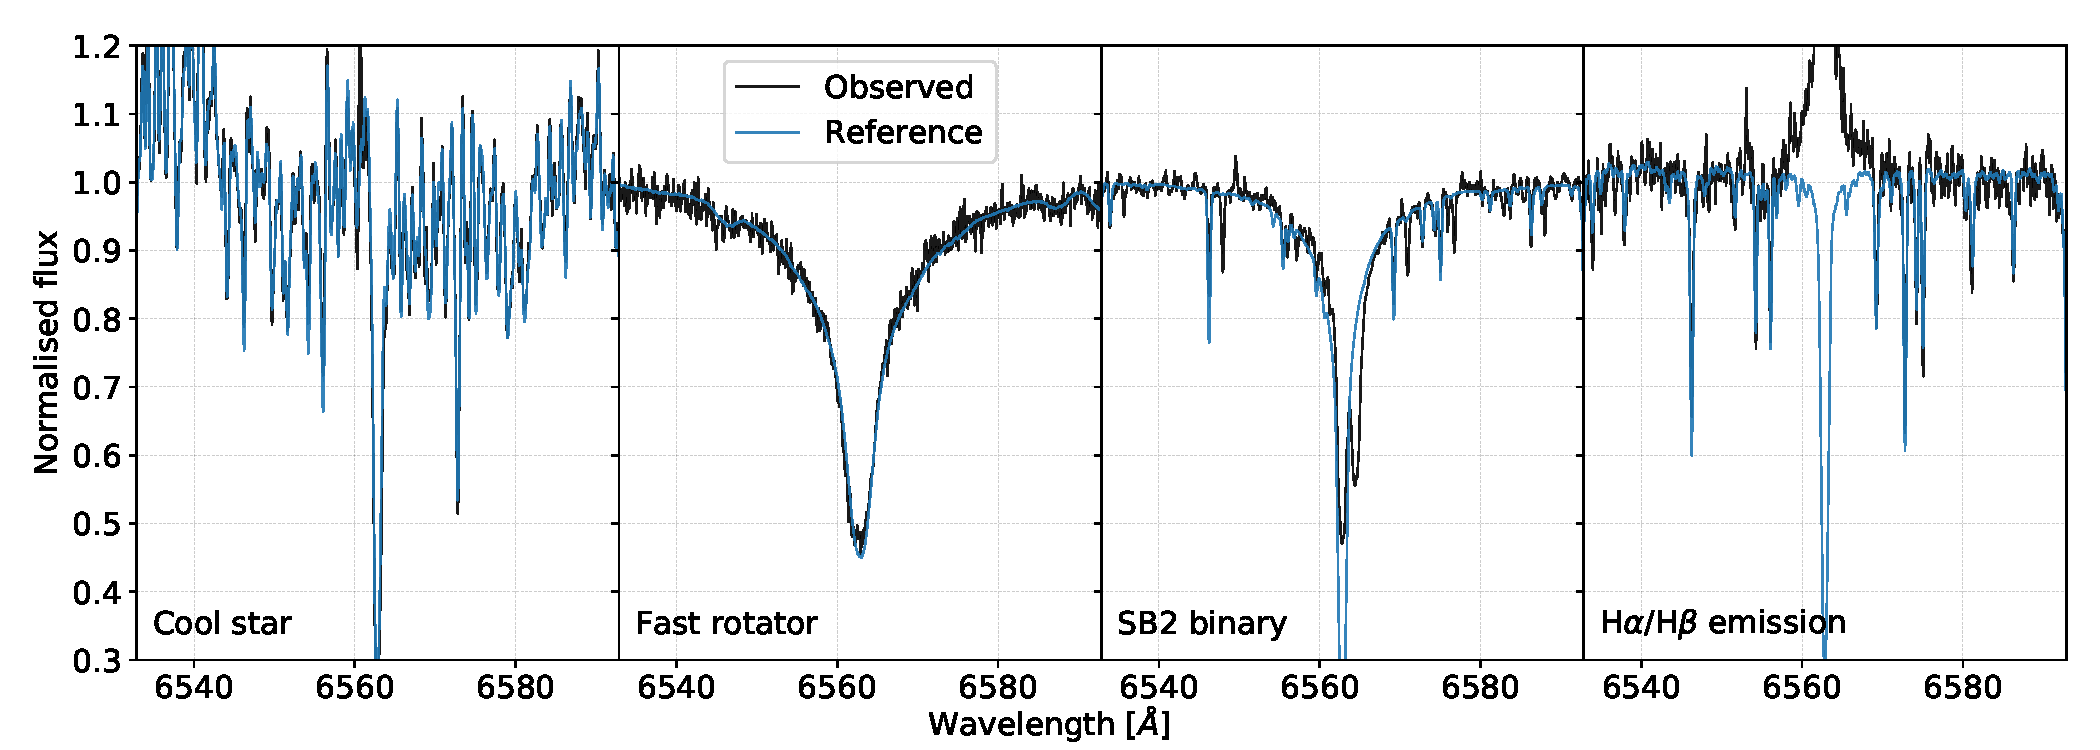
\includegraphics[width=\textwidth]{sample_spectra_spectra_ccd3.pdf}
	\caption{The diversity of spectra that must be processed by our reference spectrum generation scheme. Panels show spectra of the following normal and peculiar stars: cool, hot fast-rotating, spectroscopic binary, and H$\alpha$/H$\beta$ emission star. All examples show that the autoencoder network did reproduce the observed shapes of the normal spectra (first two) and not the peculiar spectra (last two) as desired from the reference spectrum generator. The original spectra are shown in black and reconstructed in blue.}
	\label{fig:refann}
\end{figure}

\begin{figure}
	\centering
	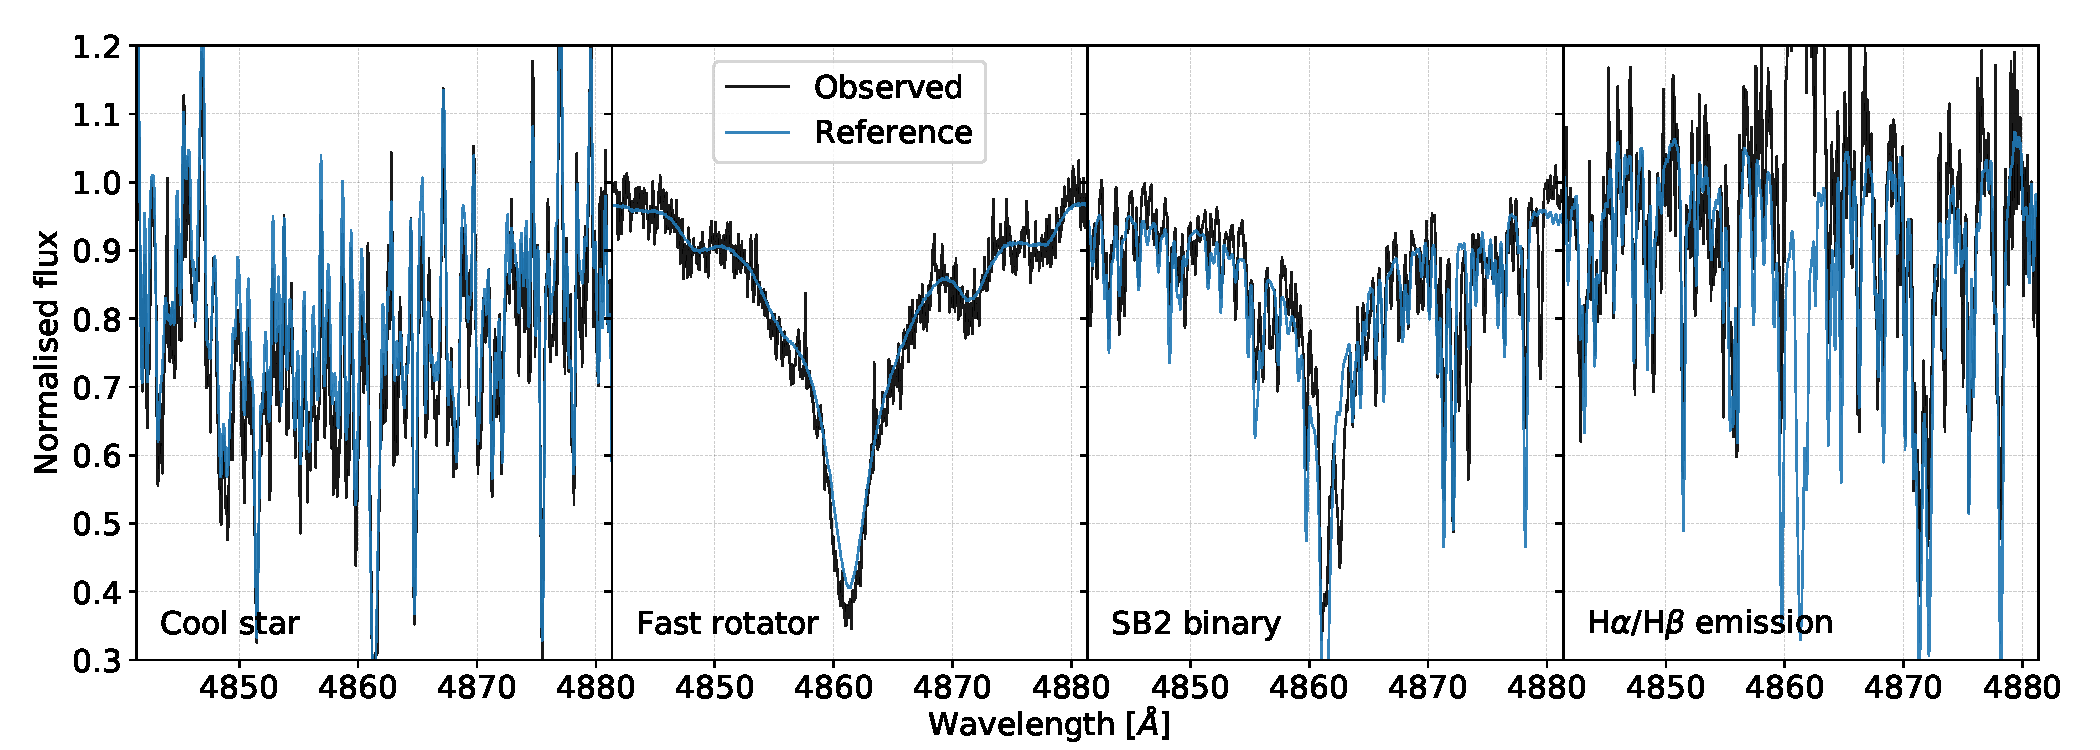
\includegraphics[width=\textwidth]{sample_spectra_spectra_ccd1.pdf}
	\caption{Same plots and objects as in Figure \ref{fig:refann} but for the blue spectral arm.}
	\label{fig:refann2}
\end{figure}

\subsection{Latent features}
To test the idea of extracted scalar latent features being connected to physical parameters, and to inspect how an autoencoder structure actually orders spectra, we colour coded values of latent features by unflagged physical parameters of input the GALAH spectra. Latent feature scatter plots, colour coded by a different combination of stellar parameters, are presented in Figures \ref{fig:latent_ccd3_1} (with \Teff\ and \Logg\ for the red arm) as well as \ref{fig:latent_ccd1_1} (with \Teff\ and \Logg\ for the blue arm) and \ref{fig:latent_ccd1_2} (with \Teff\ and \Feh\ for the blue arm).

As expected, all plots show continuous colour changes induced by the changing value of investigated physical parameter. This gives us a confirmation that the derived stellar physical parameters are spectroscopically meaningful and have the strongest influence on the appearance of acquired spectra. Rough physical parameters of previously unanalysed or peculiar spectra can therefore be acquired by averaging the parameter values of their neighborhood in the latent space. Similar procedures for parameter estimation have already been successfully explored by \citet{2015MNRAS.452..158Y, 2017ChA&A..41..318P, 2017RAA....17...36L}.

\begin{figure}
	\centering
	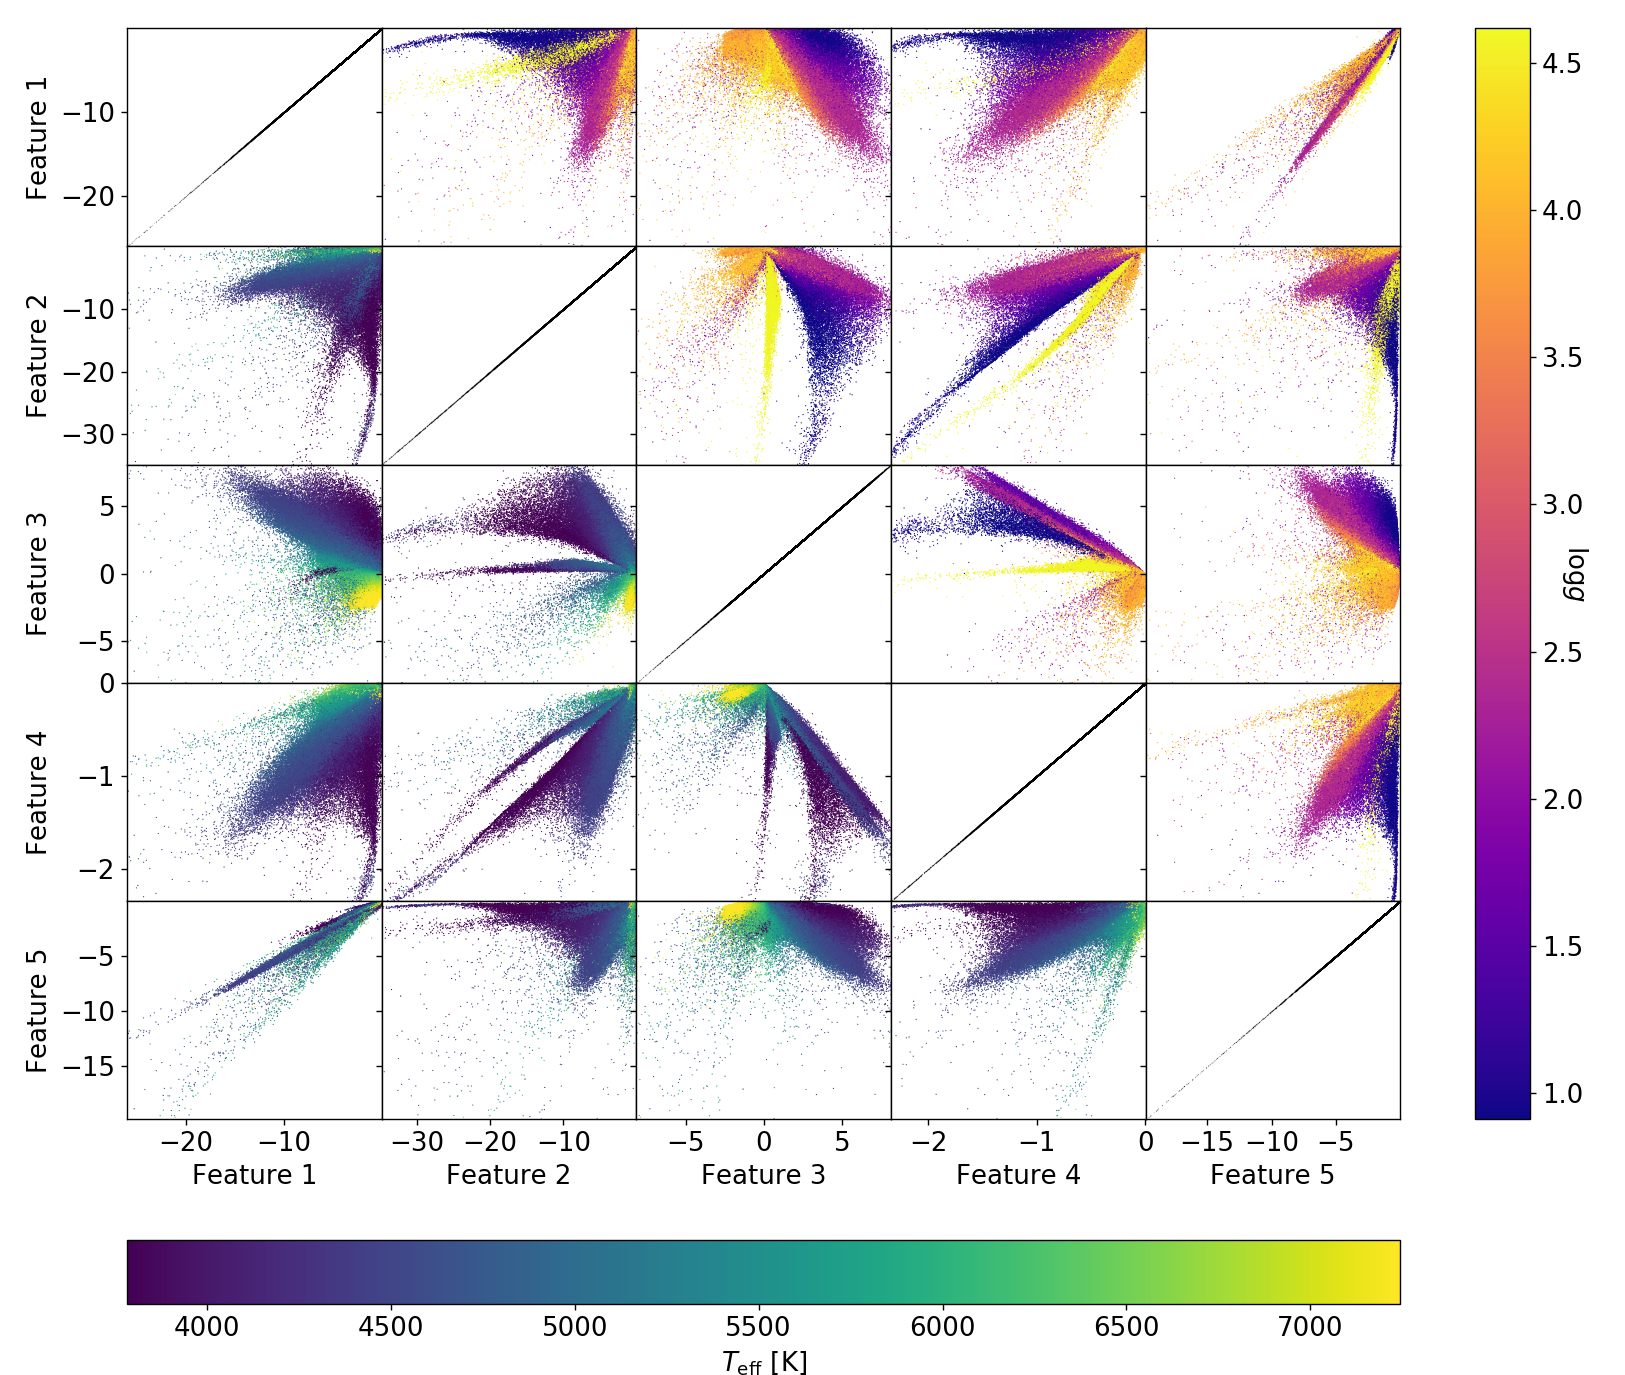
\includegraphics[width=\textwidth]{encoded_features_scatter_teff_logg_ccd3.png}
	\caption{Correlation between extracted latent features and physical parameters. Scatter plots between different features are colored by the GALAH physical parameters of original spectra. Points in the lower triangle are colored by their \Teff\ and in upper triangle by their \Logg. Associated colour mappings are given below the figure (for the lower triangle) and on its right side (for the upper triangle). Presented are results for the red arm autoencoder.}
	\label{fig:latent_ccd3_1}
\end{figure}

\begin{figure}
	\centering
	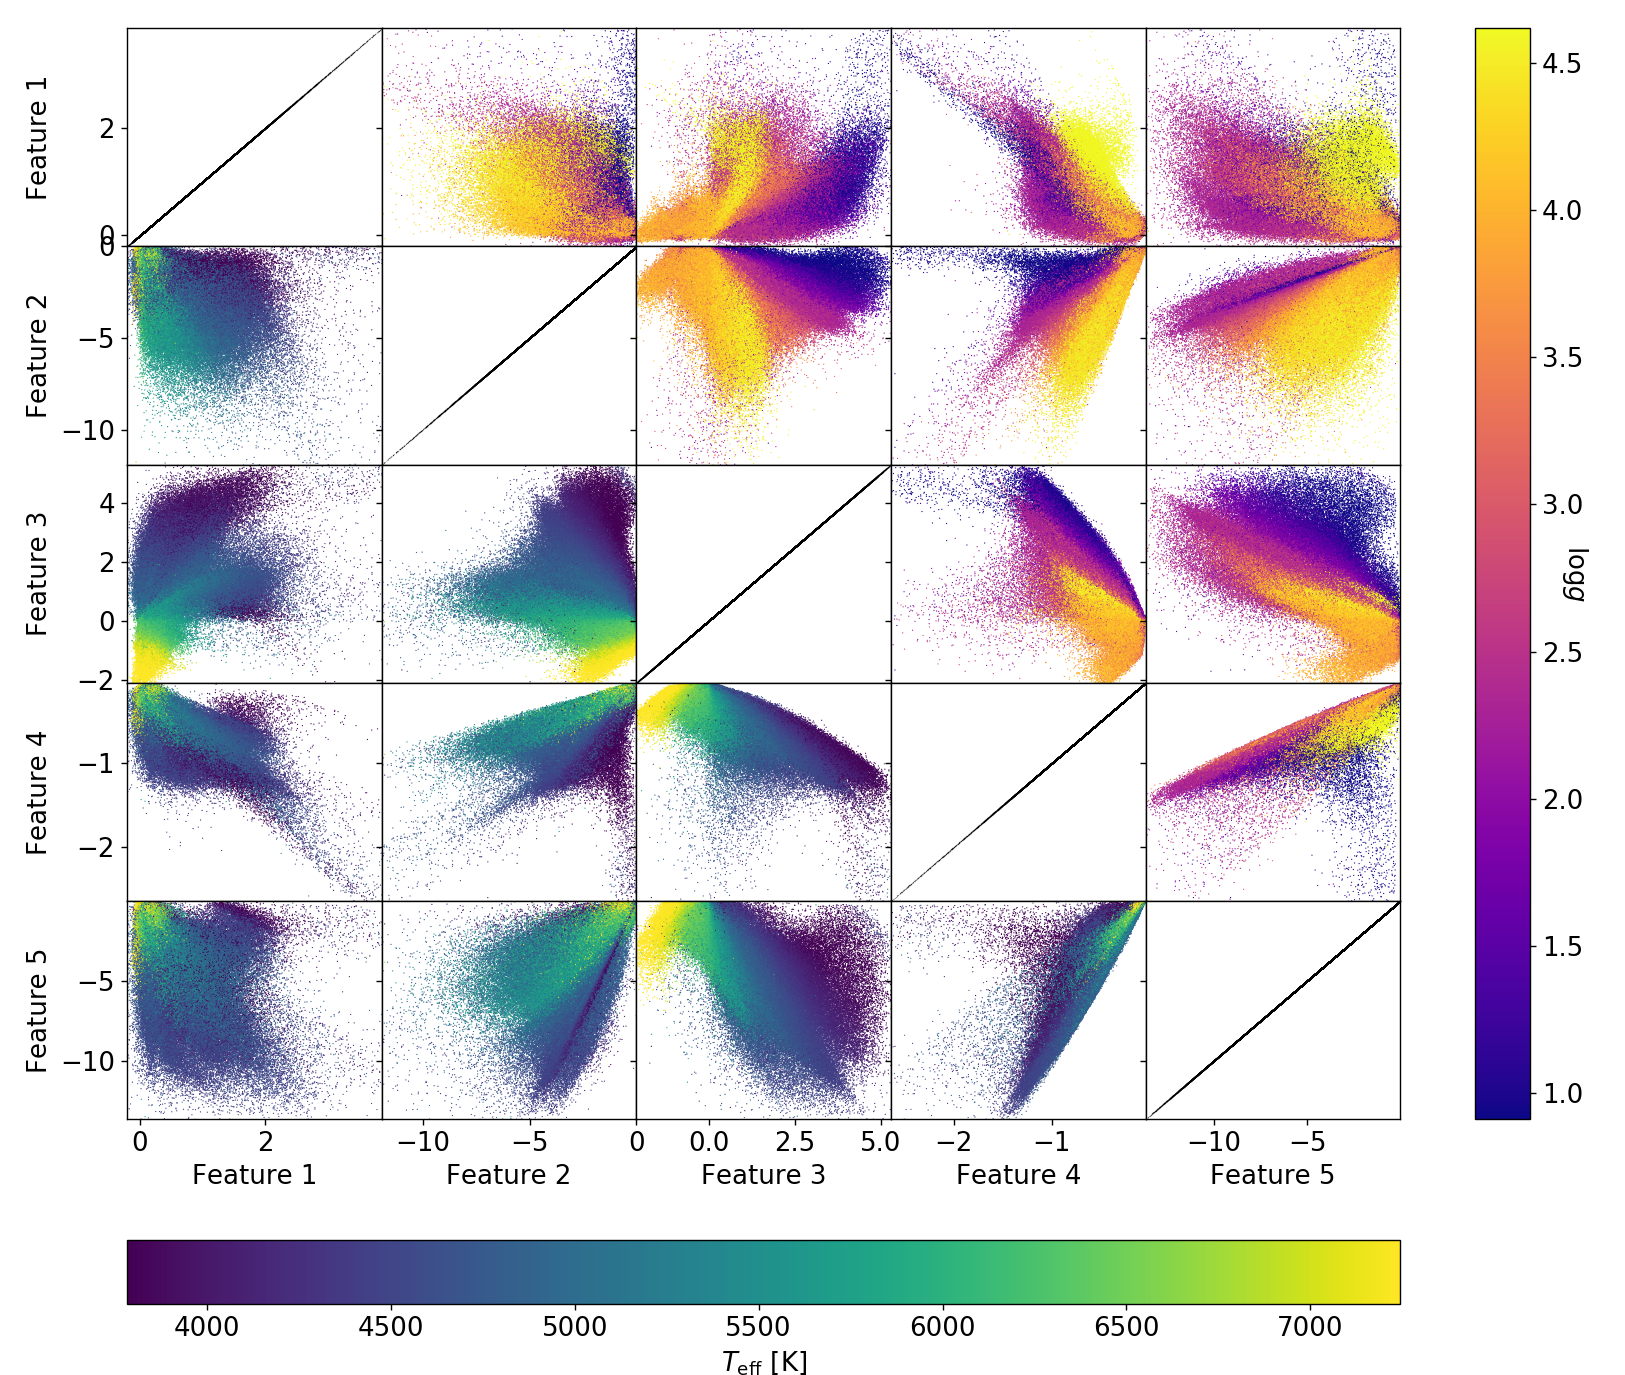
\includegraphics[width=\textwidth]{encoded_features_scatter_teff_logg_ccd1.png}
	\caption{Same plots as shown in Figure \ref{fig:latent_ccd3_1}, but for the latent features of the blue HERMES band, coloured by parameter \Teff\ on lower triangle and by \Logg\ on the upper triangle.}
	\label{fig:latent_ccd1_1}
\end{figure}

\begin{figure}
	\centering
	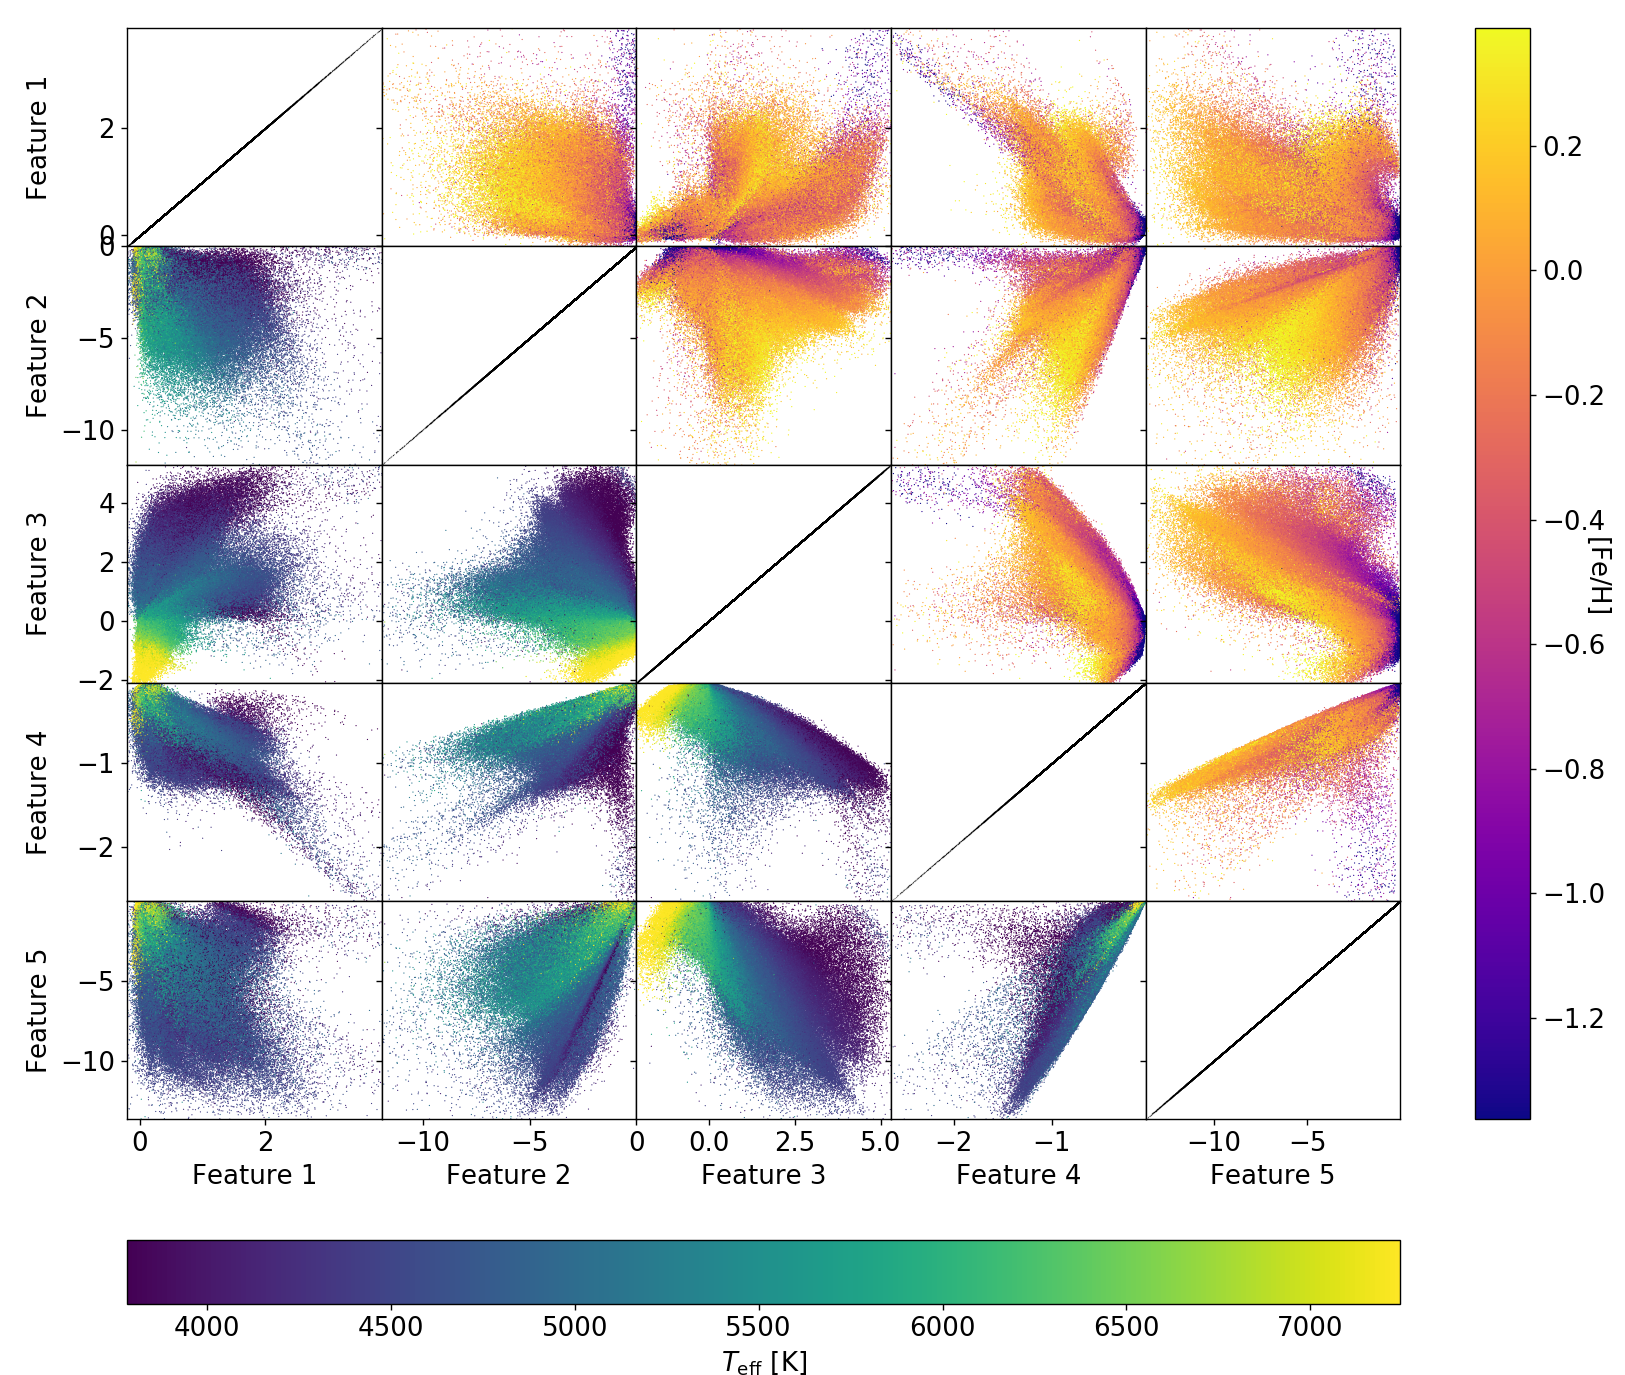
\includegraphics[width=\textwidth]{encoded_features_scatter_teff_fe_h_ccd1.png}
	\caption{Same plots as shown in Figure \ref{fig:latent_ccd3_1}, but for the latent features of the blue HERMES band, coloured by parameter \Teff\ on lower triangle and by \Feh\ on the upper triangle.}
	\label{fig:latent_ccd1_2}
\end{figure}

\subsection{H$\alpha$ and H$\beta$ emission characterization}
\label{sec:hahbemis}
The detection of emission components in spectra is based on a spectral difference $f_\mathrm{diff}$, computed as:
\begin{equation}
\label{equ:spec_diff}
f_\mathrm{diff} = f_\mathrm{obs} - f_\mathrm{ref},
\end{equation}
where $f_\mathrm{obs}$ and $f_\mathrm{ref}$ are the observed spectrum and the generated reference spectrum respectively. The result of a computed difference $f_\mathrm{diff}$ for an emission spectrum is shown in the top panel of Figure \ref{fig:emissfit}. Ideally, this computation would enhance only mismatch between both spectra, with inclusion of spectral noise, if both represent a star with the same physical stellar parameters. During the initial processing, we found out that some observed spectra have slight normalisation problems, therefore we re-normalised them prior to difference computation. As the reference spectrum $f_\mathrm{ref}$ is known and has a continuum level close to a median value of similar stars in the training set, we first compute a spectral ratio $f_\mathrm{div}$, defined as:
\begin{equation}
\label{equ:spec_div}
f_\mathrm{div} = \frac{f_\mathrm{obs}}{f_\mathrm{ref}}.
\end{equation}
The resulting ratio can be viewed as a proxy for a renormalisation curve that would bring $f_\mathrm{obs}$ to the same continuum level as $f_\mathrm{ref}$, but would at the same time cancel out any spectral differences between them. To avoid the latter, we fitted $f_\mathrm{div}$ with a $3^{rd}$ degree polynomial with a symmetrical $2$-sigma clipping, ran for five iterations. We used the polynomial fit to renormalise $f_\mathrm{obs}$.

\begin{figure}
	\centering
	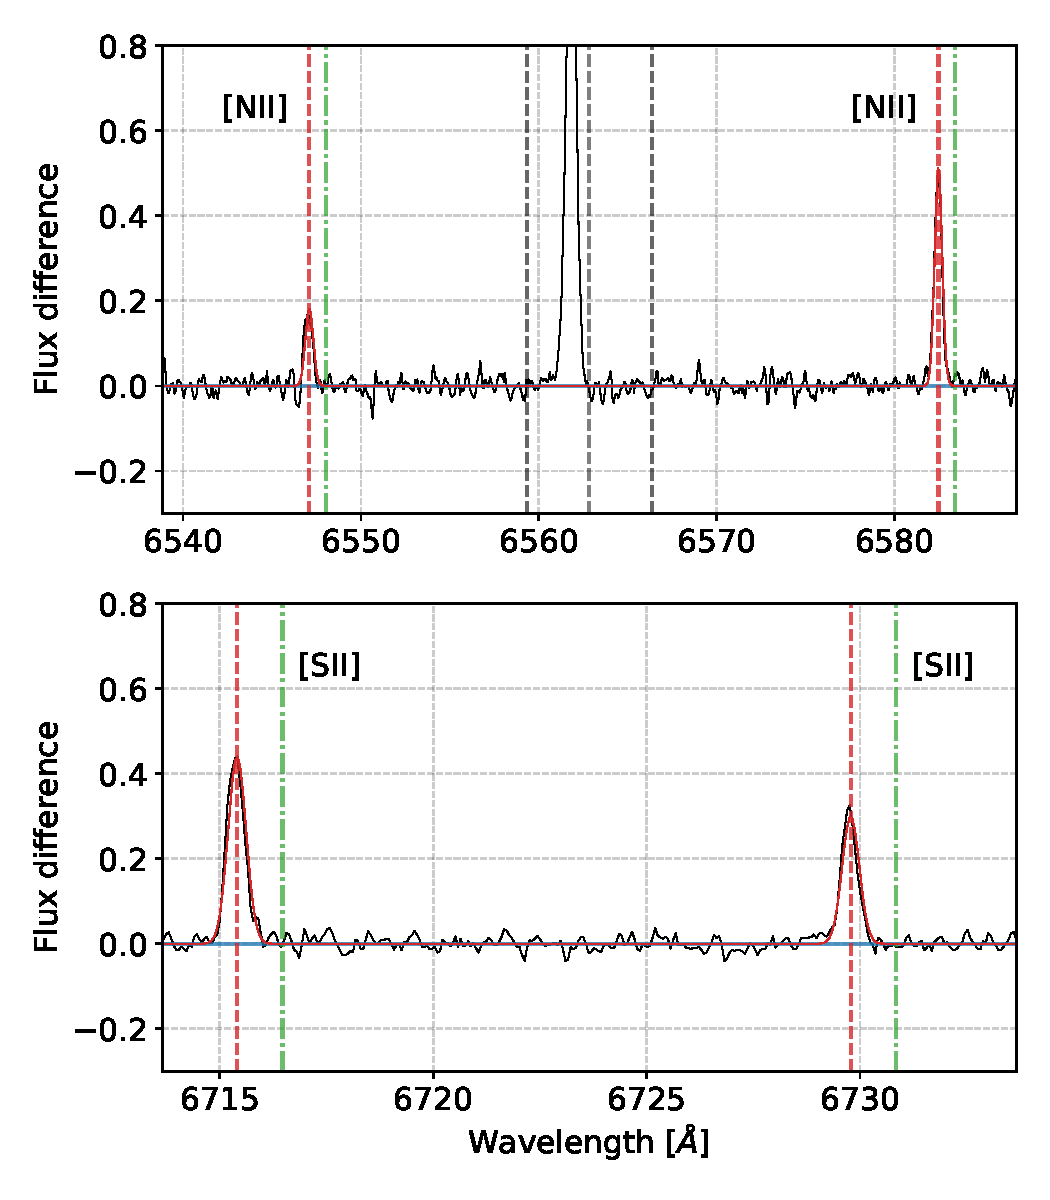
\includegraphics[width=0.6\textwidth]{paper_180131002701292_1.pdf}
	\caption{Panels show two different wavelength regions of $f_\mathrm{diff}$ for the same star. The top panel is focused on the H$\alpha$ and [NII] nebular lines, while the second panel focuses on [SII] lines. Rest wavelengths of both nebular doublets are given by the green dash-dotted vertical lines. Their fitted locations, affected by a gas cloud movement, are given by the red dashed vertical lines that both have the same radial velocity. The constant integration range around EW(H$\alpha$) is bounded by the left and right black dashed vertical lines on the top panel. The middle black dashed vertical line represents H$\alpha$ rest wavelength. All wavelengths are given in the stellar rest frame.}
	\label{fig:emissfit}
\end{figure}

To get the first identification of an emission features, we calculate the equivalent width (EW) of the spectral difference in a $\pm3.5$ \AA\ range around the investigated Balmer H$\alpha$ and H$\beta$ lines. The selected range (shown in Figure \ref{fig:emissfit}) is wide enough to encompass emission profile of all spectra, with the exception of a few, which have very broad and structured profiles. We kept the width narrow to reduce the effect of spectral noise and nearby sky emission lines (see Section \ref{sec:skyemis}). The correlation between measurements of both equivalent widths is shown in Figure \ref{fig:hab_EW} from which it is evident that the H$\beta$ emission feature is weaker than the H$\alpha$ feature. This gradual intensity reduction is a well known relation also known as the Balmer decrement. As the decrement depends on many physical parameters of stars, absorbing medium, and type of the observed object, \citet{bloom1969balmer} collected multitude of known measurements. In our case the measured ratio EW(H$\alpha$)/EW(H$\beta$) has a value close to 3/2. The ratio seems to be independent of the Balmer line strength if the emission was detected. Low EW values in Figure \ref{fig:hab_EW} should not be taken in this approximation as they are burdened by the reference model uncertainty, spectral noise, and precise continuum levels of both spectra.

\begin{figure}
	\centering
	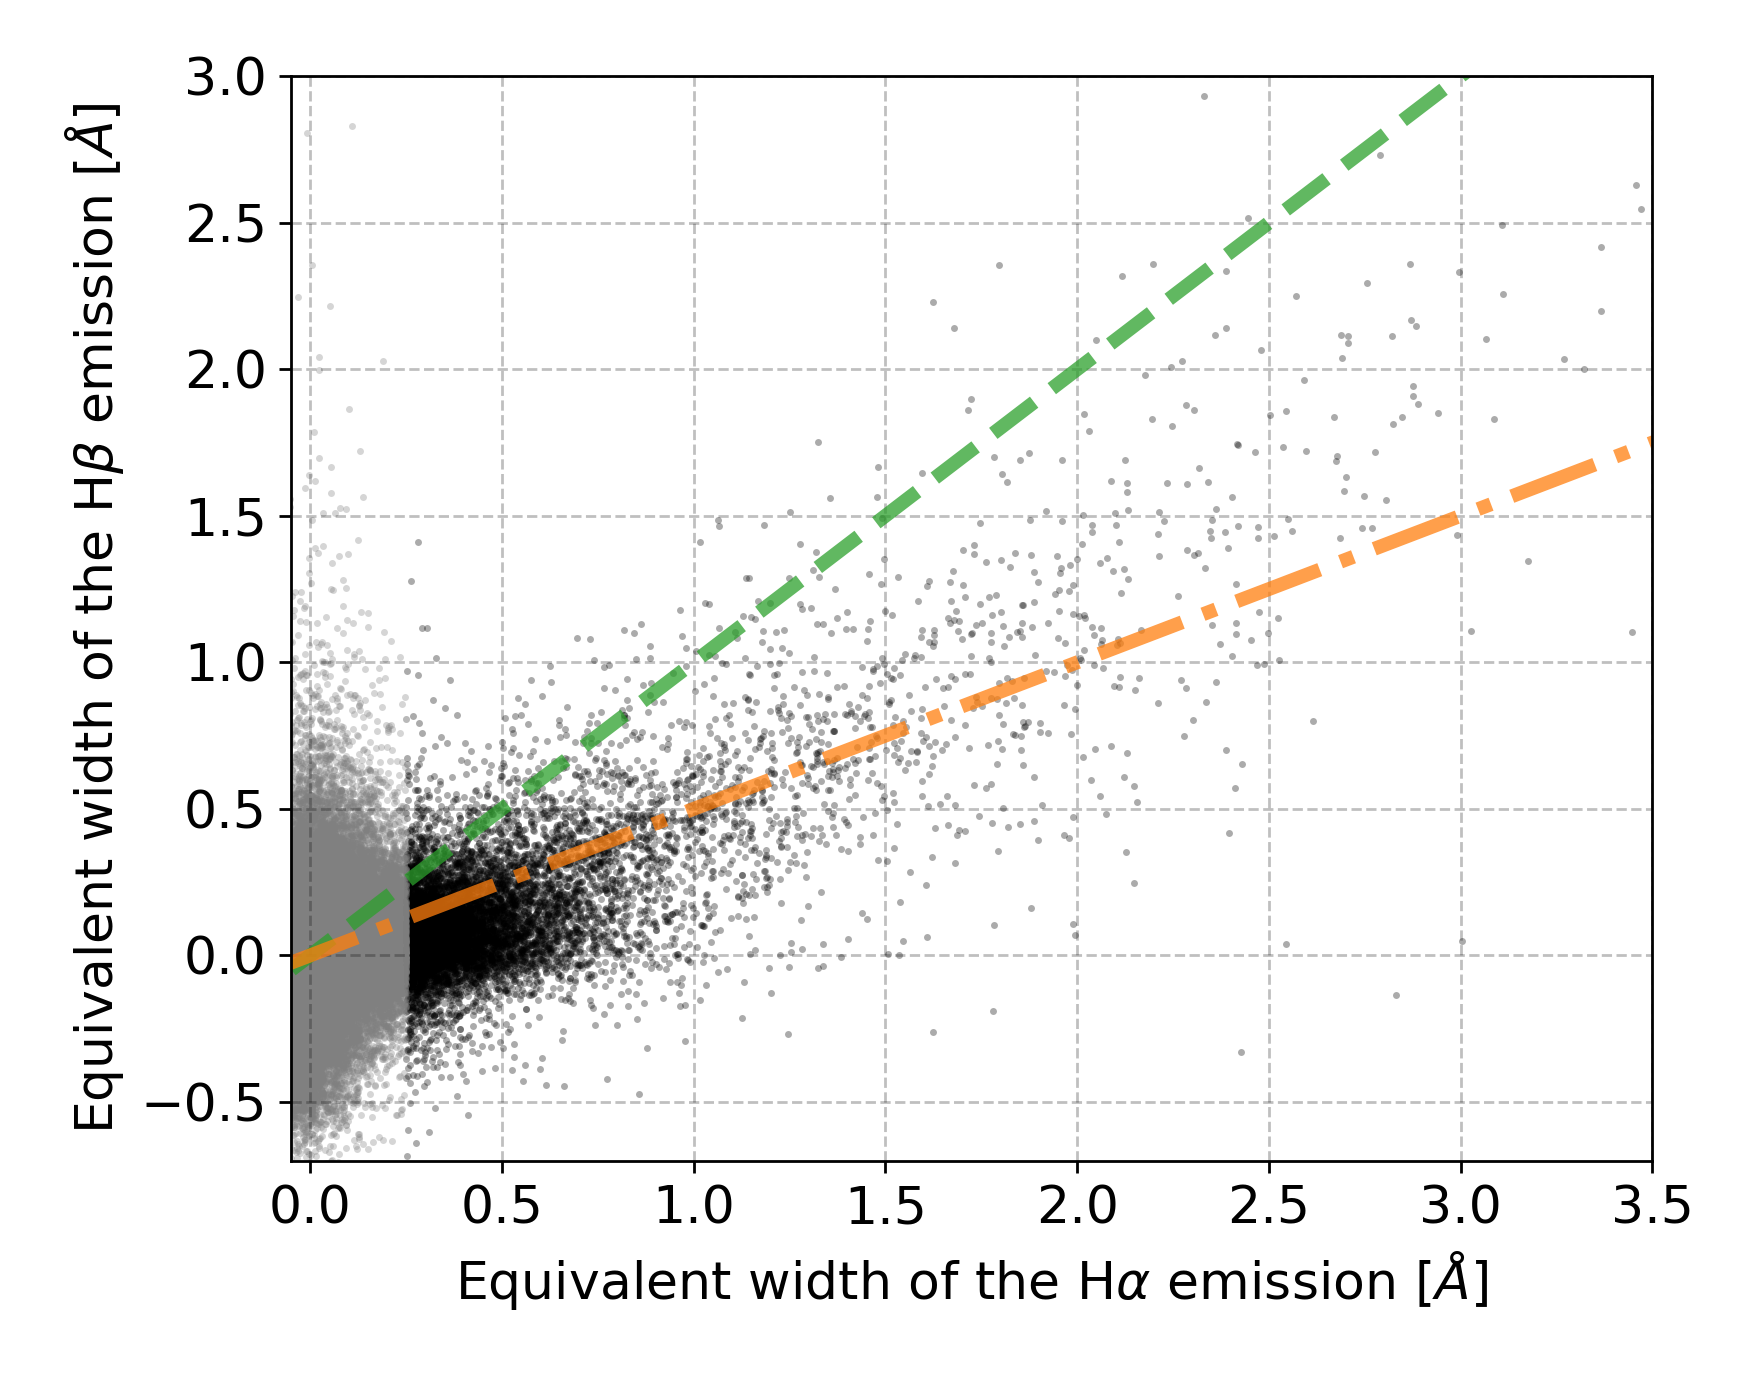
\includegraphics[width=0.6\textwidth]{H_emission_EW_dist_all.png}
	\caption{Correlation between equivalent widths of the H$\alpha$ and H$\beta$ emission components for our set of detected stars (defined as having \texttt{Ha\_EW}~>~$0.25$~\AA) as black points. The remaining set of objects is shown with gray dots. All flagged objects and possible spectroscopic binaries are taken out for this plot. The green dashed linear line represent the one-to-one relation and the orange dash-dotted line identicates cases where the equivalent width of the H$\beta$ is half of the H$\alpha$ line.}
	\label{fig:hab_EW}
\end{figure}

Alongside the equivalent widths of the residual components (EW(H$\alpha$) and EW(H$\beta$)), we also measured two additional properties of these lines, which give some insight into physical understanding of emission source. The broadening velocity of a line is described by its width at the $10$\% of the line peak (W10\%(H$\alpha$) and W10\%(H$\beta$)) expressed in \kms. The automatic measurement procedure first finds the highest point inside the integration wavelength range and then slides down on both sides of the peak until the flux drops below 10\% of the peak value. The broadening velocity is defined as a width between those two limiting cuts. As the computation is done for every object in an unsupervised way, the results are meaningful only for the spectra with evident emission lines. In the case when a low broadening velocity is estimated (equivalent to a very narrow peak), the highest peak could be a residual sky emission line or a cosmic ray streak. By combining EW(H$\alpha$) and W10\%(H$\alpha$), mass accretion could be estimated if emission is of a chromospheric origin \cite{2015A&A...575A...4F}.

The second emission line index measured in the $f_\mathrm{diff}$ spectrum, that roughly describes the shape and location of an emission feature, is the asymmetry index defined as:
\begin{equation}
\label{equ:hab_asym}
Asymmetry = \frac{|EW_\mathrm{red}| - |EW_\mathrm{blue}|}{|EW_\mathrm{red}| + |EW_\mathrm{blue}|},
\end{equation}
where $|EW_x|$ is the equivalent width of the absolute difference $|f_\mathrm{diff}|$ on the red and blue side of the rest wavelength of the investigated Balmer line. By this definition, a line that is, as a whole, moved to the redward side would have this index equal to $1$, whilst if it was moved to the blueward side, the index would instead equal $-1$. The distribution of the asymmetry index values for the most prominent and unflagged (see Section \ref{sec:flagging}) emitters is shown in Figure \ref{fig:hab_asym}, where a strong correlation between the asymmetry of H$\alpha$ and H$\beta$ lines is evident. As the H$\beta$ line in most cases produces a much weaker or even no emission feature, its asymmetry is much harder to measure. That is evident in Figure \ref{fig:hab_asym} where its index is scattered a around $0$, except for the most asymmetric cases. The distribution of the H$\alpha$ asymmetry is much more uniform outside the central symmetric region. From this index, we can roughly classify the source of the emitting component as a chromospheric origin would produce a centered component with an asymmetry index close to $0$. Everything outside the central region in Figure \ref{fig:hab_asym}, defined by the circle with a radius of $0.25$, could be thought to be of an extra-stellar origin as lines are not perfectly aligned. The used thresholding radius value of $0.25$ was defined by observing Figure \ref{fig:hab_asym} to encircle the main over-density of almost symmetric emission profiles.

\begin{figure}
	\centering
	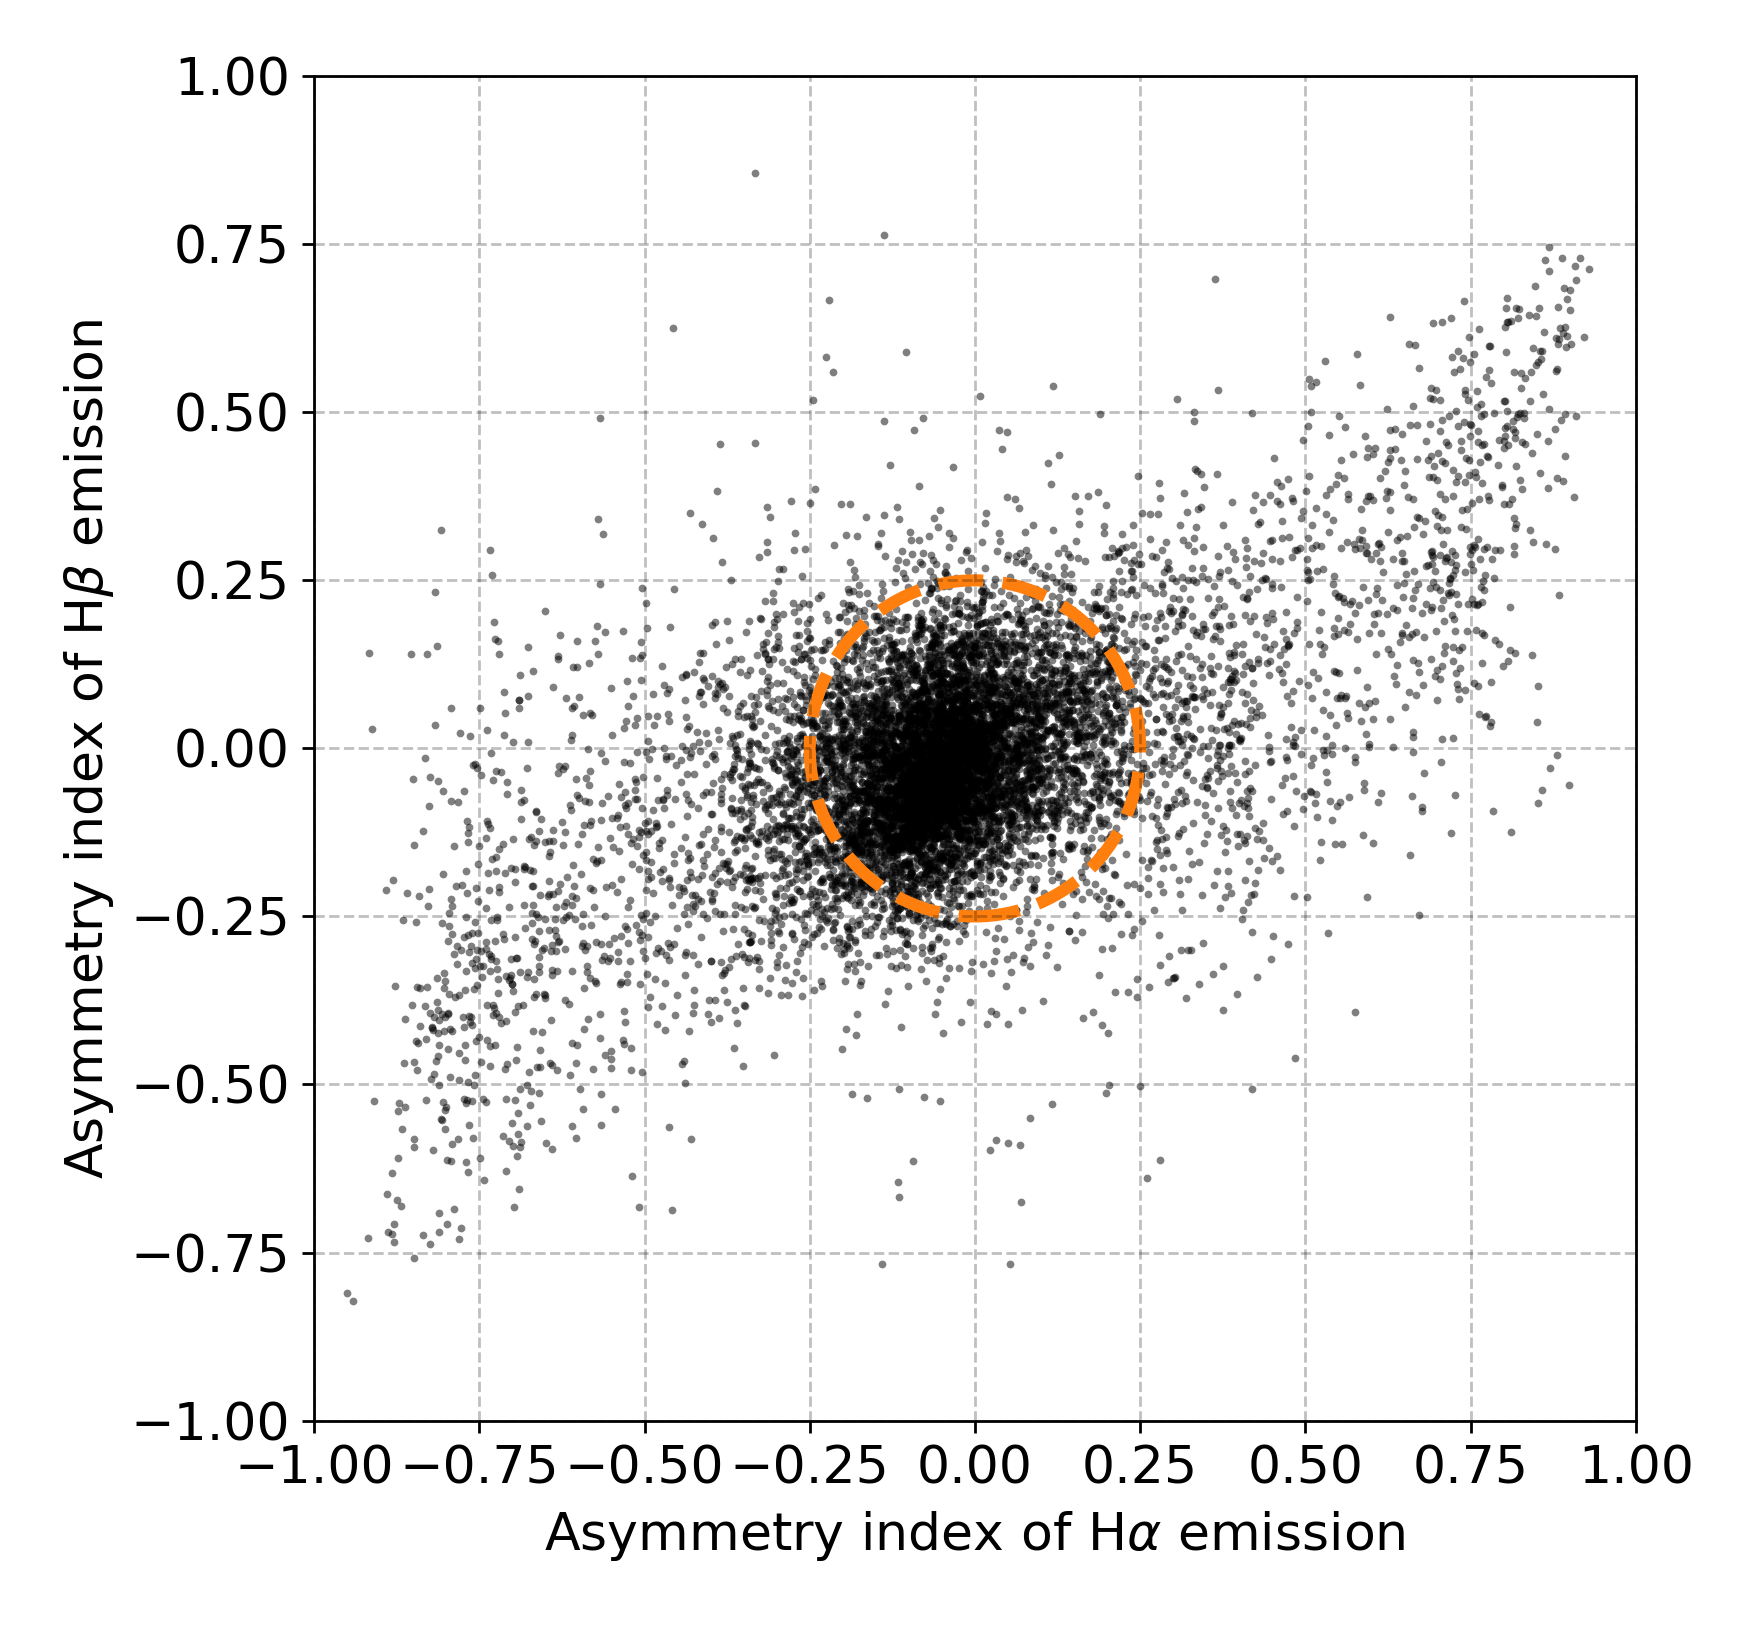
\includegraphics[width=0.6\textwidth]{H_emission_asymmetry.png}
	\caption{Asymmetry index of objects with prominent emission lines in the integration range around investigated Hydrogen Balmer lines. Objects with index inside the green dashed circle are considered to have a symmetric emission contribution, which can be attributed to a chromospheric activity. Central circular region has a radius of asymmetric index $0.25$.}
	\label{fig:hab_asym}
\end{figure}

% Like with figures 6 and 7, do we have expectations for how the data should look in figures 8 and 9? 
\begin{figure}
	\centering
	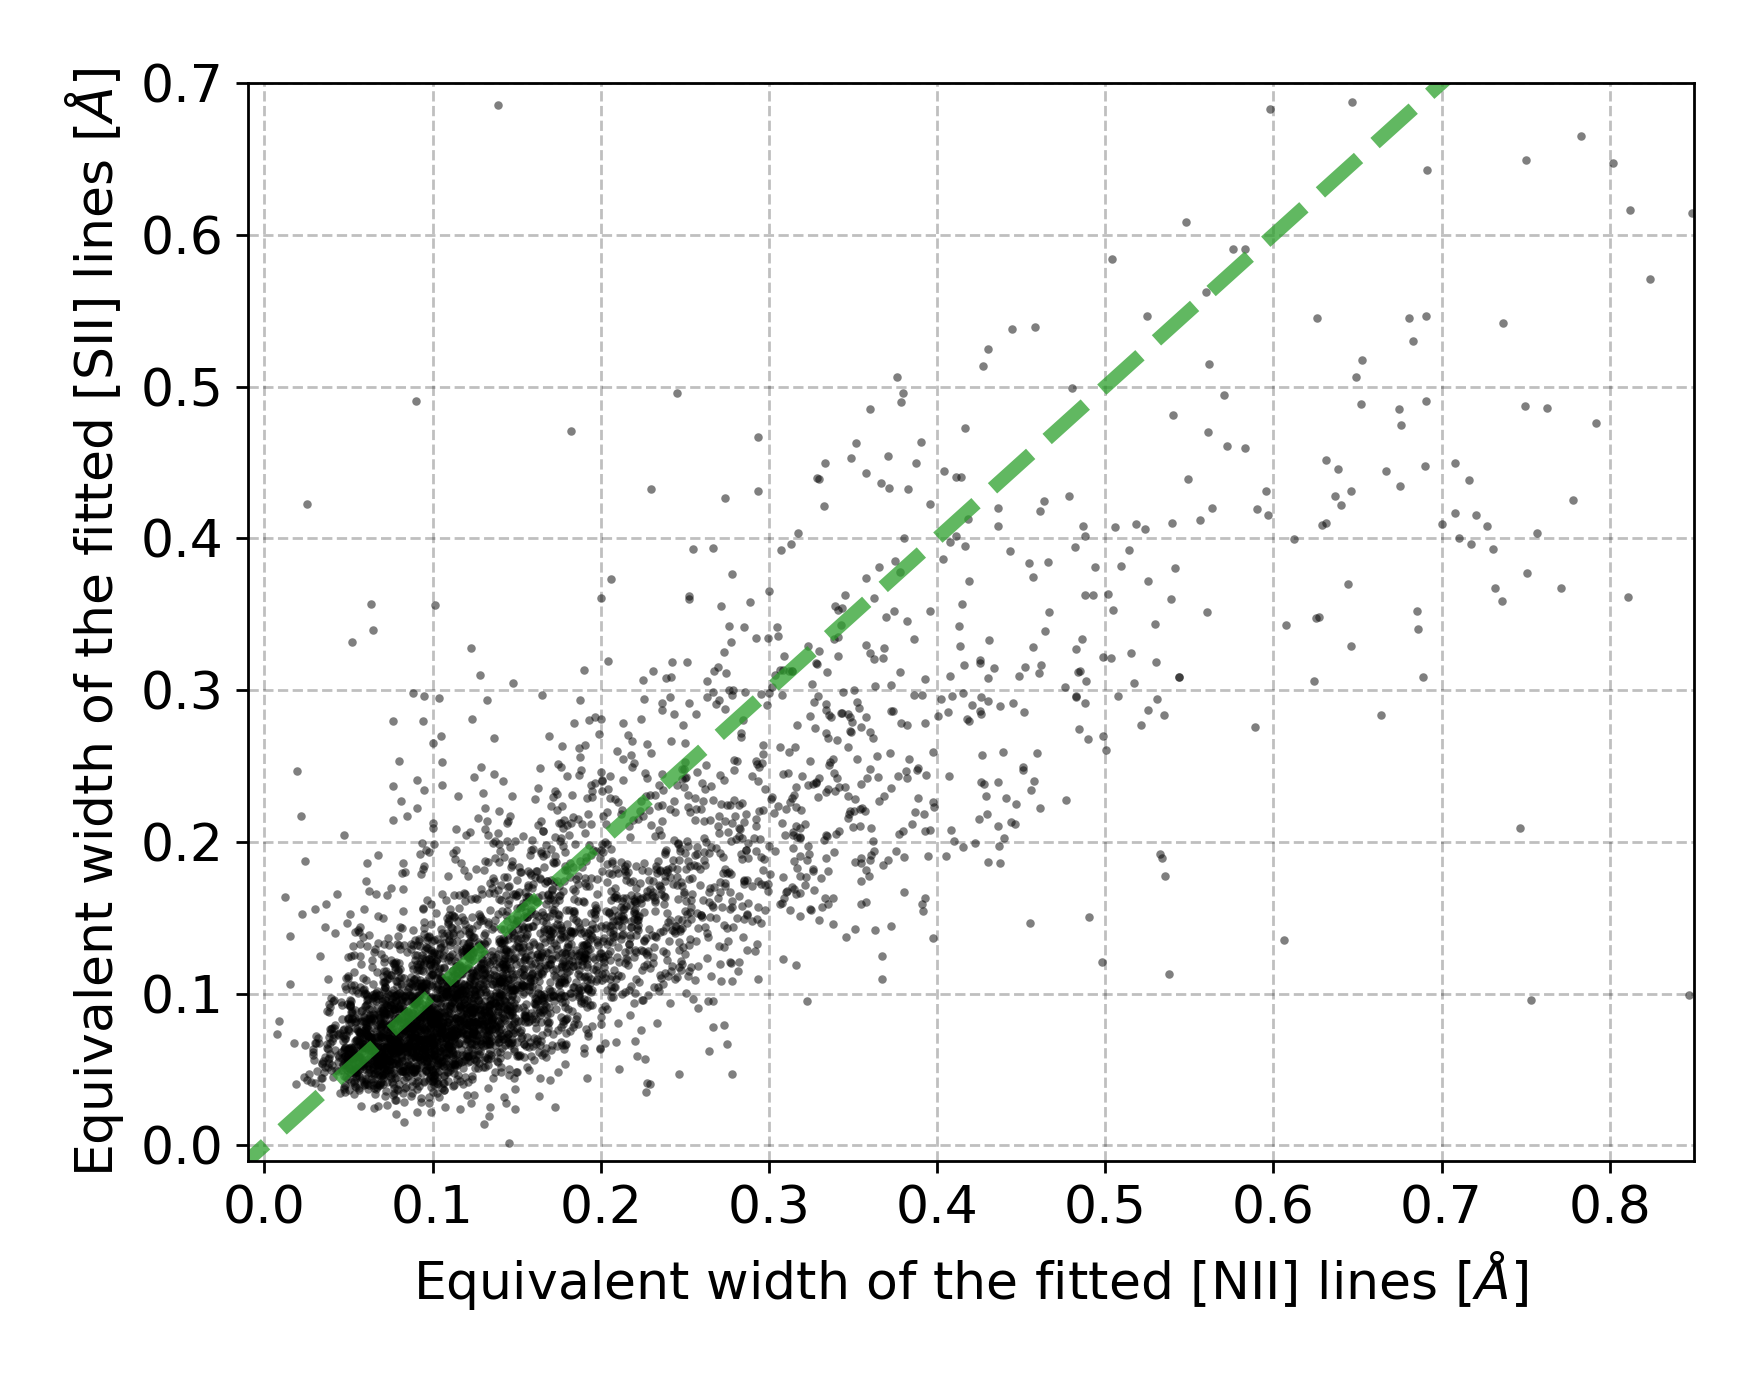
\includegraphics[width=0.6\textwidth]{sii_nii_ew_corr.png}
	\caption{Correlation between the strengths of the nebular contributions from both elements. Shown are only cases with a small difference in the determined radial velocities as shown in Figure \ref{fig:sii_nii_rv}.}
	\label{fig:sii_nii_ew}
\end{figure}

\subsection{Detection of nebular contributions}
\label{sec:nebularemis}
Due to the multiple possible origins of H emission lines \cite{2007ASSL..342.....K}, we also attempted to detect the extra-stellar nebular contributions of nearby optically thin gas. Its presence is expressed as forbidden emission lines in addition to the H emission. The spectral coverage  of the HERMES red arm enables us to observe doublets of [SII] ($6548.03$ and $6583.41$ \AA), and [NII] ($6716.47$ and $6730.85$ \AA). Having usually a weak emission contribution that could possibly be blended with nearby absorption lines, they are most easily detected when we remove the expected reference spectrum from the observed one (resulting in $f_\mathrm{diff}$). To automatically detect the emission strength and position of both doublets, we independently fitted two Gaussian functions with the same radial velocity shift for each element to $f_\mathrm{diff}$. Because the contributing medium is not necessarily physically related to the observed object, its radial velocity could be different, therefore it was treated as a free parameter in our fit. Two independent velocities, one for each of the two doublets, give us an indication of a spurious or unreliable fit component if their difference is large. To filter out outliers, we adopted a threshold of $15$~\kms\ on their velocity difference. Some of the discarded outliers might be correct detections because few of the spectra show two or more peaks for each nebular line which might point to a contribution of multiple clouds with different radial velocities. Such cases are not fully accounted for by the fitting algorithm that only identifies the strongest emission.

\begin{figure}
	\centering
	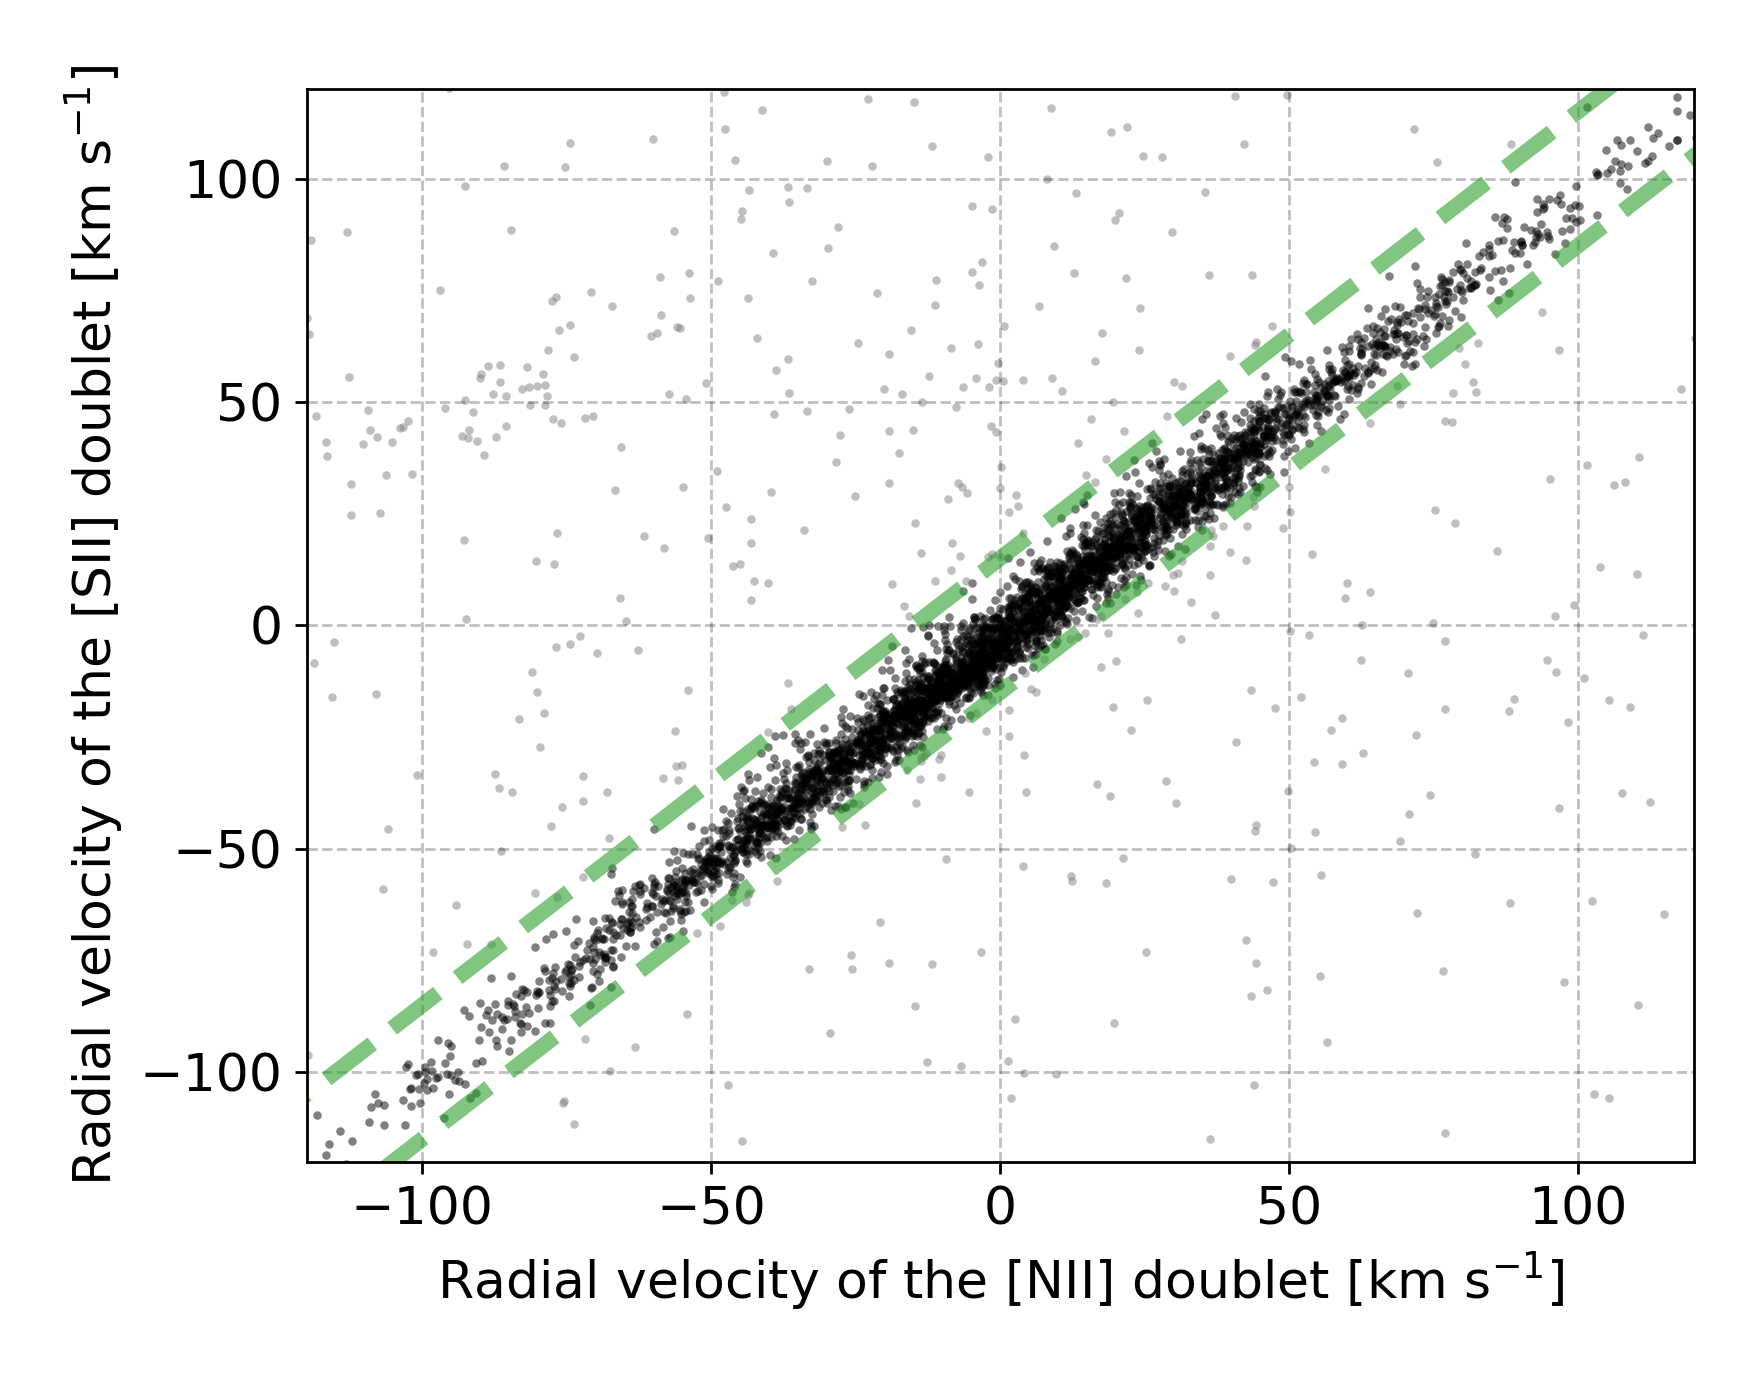
\includegraphics[width=0.6\textwidth]{sii_nii_rv.png}
	\caption{Correlation between radial velocity of both assessed nebular contributions that are observable in the red arm of the HERMES spectrum. Shown are only cases with at least three detected forbidden lines. The grey dots were further discarded as their absolute difference between velocities is more than $15$~\kms. The limiting thresholds are visualized by dashed linear lines. Plotted velocities are measured in the stellar rest frame and therefore grouped towards zero velocity, meaning they are moving together with the star. Velocity distributions of selected measurements are presented around the main scatter plot.}
	\label{fig:sii_nii_rv}
\end{figure}

In the absence of additional fitting constraints, the routine might also find two noise peaks and lock onto them. Therefore, we put an arbitrarily selected detection threshold ($0.05$ of relative flux) on a minimum amplitude of the fitted forbidden lines to be counted as detected. The result from this fitting and analysis procedure is a number of successfully detected peaks per element and their combined equivalent widths (EW([NII]) and EW([SII])), reported in the final published table (Table \ref{tab:results}). To filter out some possible miss-detection, we count a spectrum as having nebular lines when at least three nebular lines above the threshold were detected. The correlations for measured radial velocities and equivalent widths of identified objects with nebular emission are given in Figure \ref{fig:sii_nii_ew} and \ref{fig:sii_nii_rv} respectively.

The radial velocities of both doublets shown in Figure \ref{fig:sii_nii_rv} give us a first impression that the gas dynamics of the elements in all observed clouds is nearly coincident, but elements are moving at slightly different velocities. This velocity offset, but in the opposite direction, was also observed by \citet{2016A&A...591A..74D, 2017A&A...604A.135D} who attributed it to the uncertainties in their adopted line wavelengths, that are slightly different to ours (less than $0.05$~\AA), causing the velocity points to be located either above or under the identity line in Figure \ref{fig:sii_nii_rv}. Additionally, the plot reveals that the majority of the gas clouds have a different radial velocity than stars behind or inside a cloud.

As we are working with fully reduced normalised spectra, with inclusion of sky background removal, the detection procedure would, in the case of an ideal background removal, not detect emission due to nebular clouds. As the measured flux of the nebular contribution is very unlikely the same for object and because of the physical separation of the sky fibres (see next Section \ref{sec:skyemis} and \citet{2017MNRAS.464.1259K}), the ideal cases are very rare. Similarly, the densities and the temperatures of such nebular clouds, extracted from corrected spectra could be influenced by the extraction pipeline and were therefore not performed in our case. 

\begin{figure}
	\centering
	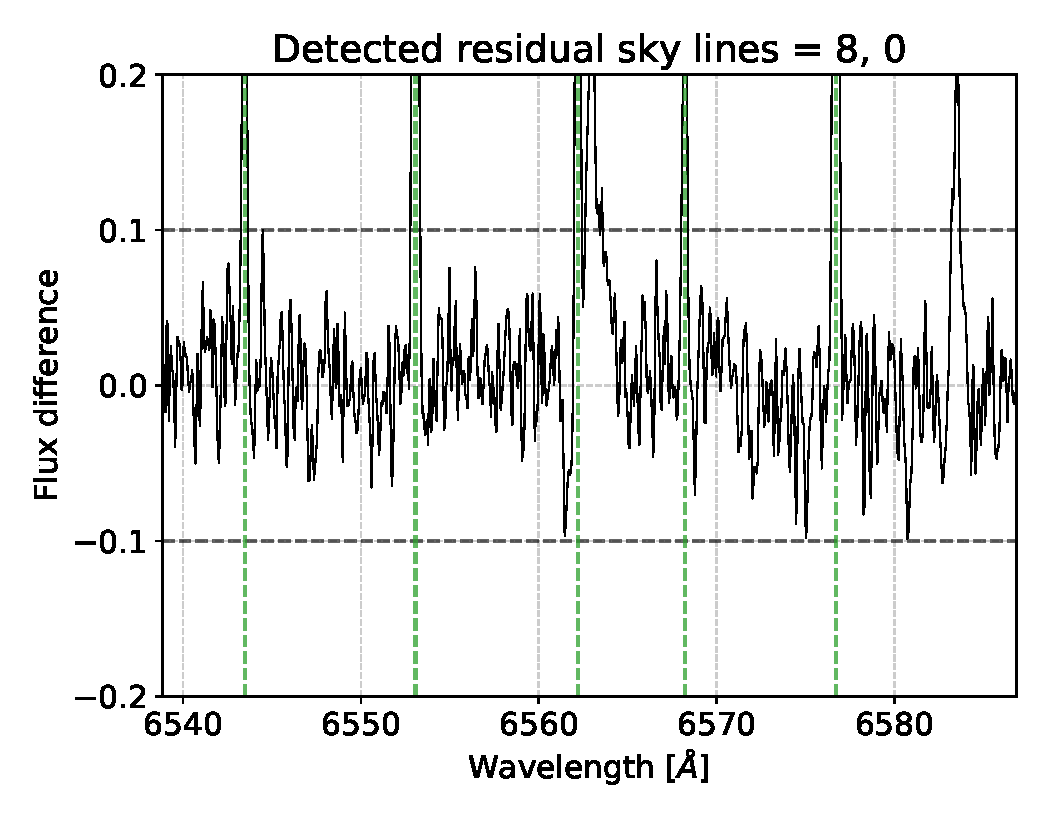
\includegraphics[width=0.6\textwidth]{paper_170509002201287_2.pdf}
	\caption{Sky emission lines are most evident after spectra subtraction in $f_\mathrm{diff}$. Green vertical dashed lines represent expected locations of emission lines in the rest frame of an observed star. The middle sky line in this plot falls inside the actual H$\alpha$ emission feature and changes its shape from single- to double-peaked and consequently modifies the measured equivalent width. Upper and lower thresholds for detection are given by the bold horizontal dashed lines. The number of detected under- and over-corrected sky lines in this order is given above the plot.}
	\label{fig:skyemiss}
\end{figure}

The strength of the identified lines, measured by their equivalent widths, is shown in Figure \ref{fig:sii_nii_ew}. This shows a high degree of correlation, where on average [SII] lines have lower strength than [NII] lines. Rough estimation of ratio between their measured equivalent widths EW([NII])/EW([SII]) is close to the value of 4/3.

\subsection{Identification of sky emission lines}
\label{sec:skyemis}
Attributing a limited and relatively low number of the HERMES fibres to monitor the sky in hopefully star and galaxy free regions, imposes limitations to a quality of the sky background removal in the GALAH reduction pipeline \cite{2017MNRAS.464.1259K}. As the sky spectrum is sampled at $25$ distinct locations over the whole $2^\circ$ diameter field, it must be interpolated for all other fibre locations that are pointing towards stellar sources. Depending on the temporal and spatial variability of weather conditions, and possible nebular contributions, interpolation may produce an incorrect sky spectrum that is thereafter removed from the observed stellar spectra.

In most cases, this does not influence the spectral analysis, unless one of the strongest sky emission lines falls in a range of the analysed stellar line. For us, the most problematic sky emission line, which can alter the shape of the H$\alpha$ profile, is located at $6562.7598$~\AA\ (used list of sky emission lines was taken from \citet{2003A&A...407.1157H}). Being close to the adopted wavelength of the H$\alpha$ ($6562.8518$~\AA), it can get blended with a real emission feature or simulate its presence. We tried to estimate the impact of the sky residual in the spectrum from multiple nearby emission lines. First, we select only the strongest sky emitters (with parameter \texttt{Flux}~$\ge$~$0.9$ in \citet{2003A&A...407.1157H}) and shift their reference wavelength into a stellar rest frame. After that, we use a simple thresholding (see Figure \ref{fig:skyemiss}) to estimate their number. By the thresholding procedure, we want to simultaneously catch over- and under-corrected stellar spectra.

When a sufficient number ($\ge$~$4$) of strong residual sky lines with a normalised flux above $10$\% is detected, a quality flag (see Section \ref{sec:flagging}) is raised, warning a user that the equivalent width of the H$\alpha$ emission could be affected by uncorrected sky emission. As this potential contamination is present only in the red HERMES arm, we do not check for spurious strong emitters in the region around the H$\beta$ line.

\begin{figure}
	\centering
	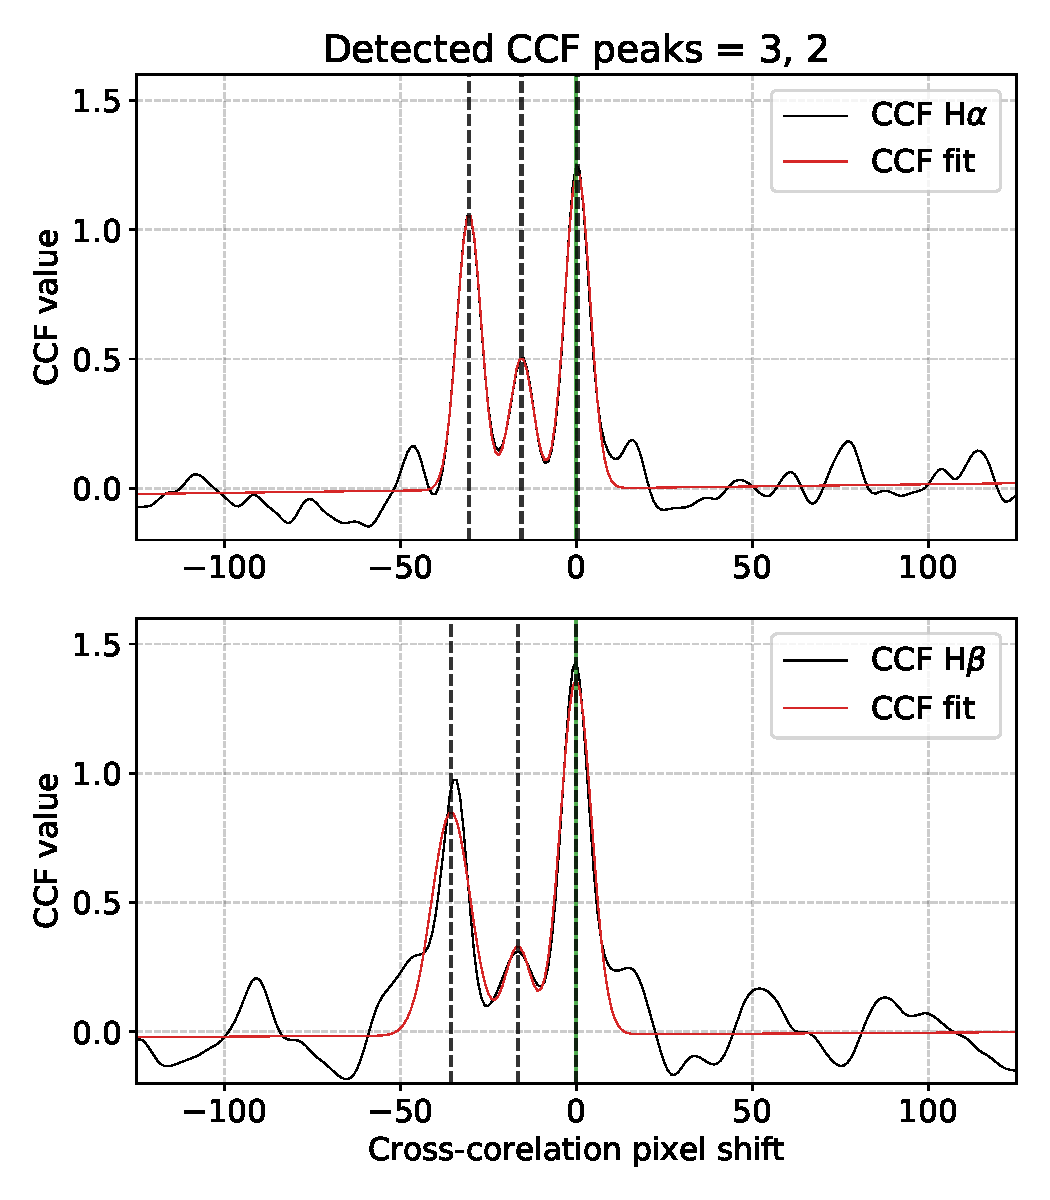
\includegraphics[width=0.6\textwidth]{paper_140812003801021_3.pdf}
	\caption{Detection of a spectroscopic binary candidate by cross-correlating observed spectrum with its reference spectrum. Three Gaussian functions that are fitted to the resulting CCF (black solid curve) are depicted by their means (dashed vertical lines) and their best fitting sum in red. Presented are CCFs for the red arm in the top panel and for the blue arm in the bottom panel. Number of detected peaks for both arms is given above the figure. The middle marked peak in the bottom plot was not detected due to its low fitted amplitude that could hint to a feature caused by a spectral noise. Peaks of similar amplitude, that could cause wrong binarity determination, are seen left and right of central CCF region.}
	\label{fig:sb2ccf}
\end{figure}

\subsection{Determination of spectral binarity}
During the inspection of our initial results, we noticed that the spectra of spectroscopically resolved binary stars (SB2) produce a mismatch between observed and reference spectra whose $f_\mathrm{diff}$ have a profile similar to the P Cygni or inverted P Cygni profile \cite{1979ApJS...39..481C} that is often observed in emission-line objects. To detect SB2 candidates, we performed cross-correlation between the reference and the observed spectra, disregarding the wavelength range of $\pm10$\AA\ around the centre of the Balmer lines to avoid broadening of the cross-correlation function (CCF) peak. Cross-correlation was performed independently for both (the blue and red) HERMES spectral arms. The resulting CCF, shown as the black curve in Figure \ref{fig:sb2ccf}, was fitted by three Gaussian functions, centred at three strongest peaks, to describe its shape. The location, amplitude and width of those peaks were assessed to determine the number of stellar components in the spectrum. When fitting three peaks, there is a possibility of finding triple stars and distinguishing them from binaries. Every spectral arm with more than one prominent peak was marked as potential SB2 detection in the final results (see Table \ref{tab:results}), where binarity indication is given independently for both arms. Nevertheless, the results of the blue arm (column \texttt{SB2\_c1}) are more trustworthy because of the higher number of absorption lines in the red arm (column \texttt{SB2\_c3}). For even greater completeness of detected SB2 candidates, a list of analyzed binaries, compiled by \citet{2020arXiv200500014T} can be used. They combined unsupervised spectral dimensionality reduction algorithm t-SNE and semi-supervised CCF analysis \cite{2017A&A...608A..95M} to compile their list of SB2 binaries. After their analysis, they discarded spectra that were falsely identified as SB2 by their detection procedures.

An unexpected result of this binarity search was the realization that some reduced spectra show duplicated lines only in the red arm or even stranger, only in a smaller subsection of it. After a thorough investigation, we uncovered that this effect is caused by improper treatment of fibre cross-talk while extracting spectra from the original 2D image \cite{2017MNRAS.464.1259K}. A partial culprit of this is also a poorer focus in the red arm. Therefore if only flag \texttt{SB2\_c3} is set, and not \texttt{SB2\_c1}, this can be used as an indication of the above reduction effect.

Additionally, the highest peak of our CCF function is used to determine the correctness of the wavelength calibration during the reduction of the spectra \cite{2017MNRAS.464.1259K}. If the peak is shifted by more than five correlation steps (maximum shift equals to about 13~\kms) from the rest wavelength of the reference spectrum, the quality flag (see Section \ref{sec:flagging}) is raised, warning the user that the derived radial velocity, equivalent width, and asymmetry index might be wrong in the respective arm as both spectra were not aligned ideally.

\subsection{Resulting table}
\label{sec:results}
The emission indices and other computed parameters are collected in Table \ref{tab:results}. The complete table is available in electronic form at the CDS. An excerpt of the published results, containing a subset of 30 rows and 11 most interesting columns for the strongest unflagged emitters is given in Table \ref{tab:results_values}.

\begin{table}
	\centering
	\caption{List and description of the fields in the published catalogue of analysed the GALAH spectra.}
	\label{tab:results}
	\begin{tabular}{l c l}
		\hline
		Column & Unit & Description \\
		\hline \hline
		\texttt{source\_id} & & \G\ DR2 star identifier \\
		\texttt{sobject\_id} & & GALAH internal per-spectrum unique id \\
		\texttt{ra} & deg & Right ascension coordinate from Two Micron All-Sky Survey (2MASS, \cite{2006AJ....131.1163S})\\
		\texttt{dec} & deg & Declination coordinate from 2MASS\\
		\texttt{Ha\_EW} & \AA & Equivalent width of a difference between observed \\
		& & and template spectrum in the range of $\pm3.5$~\AA\ \\
		& & around the H$\alpha$ line \\
		\texttt{Hb\_EW} & \AA & Same as the \texttt{Ha\_EW}, but for the H$\beta$ line \\
		\texttt{Ha\_EW\_abs} & \AA & Equivalent width of an absolute difference between \\
		& & observed and template spectrum in the range of \\
		& & $\pm3.5$~\AA\ around the H$\alpha$ line \\
		\texttt{Hb\_EW\_abs} & \AA & Same as the \texttt{Ha\_EW\_abs}, but for the H$\beta$ line\\
		\texttt{Ha\_W10} & \kms & Width (in \kms) of the H$\alpha$ emission feature at \\
		& & $10$\% of its peak flux amplitude \\
		\texttt{Ha\_EW\_asym} & & Value of asymmetry index for the H$\alpha$ line \\
		\texttt{Hb\_EW\_asym} & & Value of asymmetry index for the H$\beta$ line \\
		\texttt{SB2\_c3} & & Was binarity detected in the red arm \\
		\texttt{SB2\_c1} & & Was binarity detected in the blue arm \\
		\texttt{NII} & & Number of detected [NII] peaks in the doublet \\
		\texttt{SII} & & Number of detected [SII] peaks in the doublet \\
		\texttt{NII\_EW} & \AA & Combined equivalent width of a fitted Gaussian profiles \\
		& & to both studied [NII] emission features \\
		\texttt{SII\_EW} & \AA & Same as the \texttt{NII\_EW}, but for the [SII] doublet \\
		\texttt{rv\_NII} & \kms & Intrinsic radial velocity of the [NII] doublet, \\
		& & corrected for the barycentric and stellar velocity \\
		\texttt{rv\_SII} & \kms & Same as \texttt{rv\_NII}, but for the [SII] doublet \\
		\texttt{nebular} & & Is spectrum considered to have an additional \\
		& & nebular component \\
		\texttt{emiss} & & Is spectrum considered to have an additional H$\alpha$ \\
		& & emission component \\
		\texttt{flag} & & Sum of all bitwise flags raised for a spectrum \\
		\hline
	\end{tabular}
\end{table}

As we do not perform any quality cuts on our results, a suggested set of limiting parameter thresholds and quality flags is provided in Section \ref{sec:flagging}. Their use depends on user-specific requirements and the analysed science case.

\begin{sidewaystable}
	\centering
	\caption{Excerpt of 30 strongest unflagged emitters from the published table presented in detail by Table \ref{tab:results}. The rest of the table can be downloaded in electronic form CDS service and publishers' website.}
	\label{tab:results_values}
	\begin{tabular}{c c c c c c c c c c c}
		\hline
		source\_id & Ha\_EW & Ha\_EW\_abs & Ha\_W10 & Ha\_EW\_asym & NII & SII & NII\_EW & rv\_NII & rv\_SII & flag \\
		\hline \hline
		3337923100687567872 & 5.37 & 5.37 & 373.63 & 0.36 & 1 & 0 & 0.05 & -30.22 & 23.54 & 0 \\
		3217769470732793856 & 5.06 & 5.06 & 252.48 & 0.07 & 0 & 1 & 0.01 & -11.32 & 35.71 & 0 \\
		4660266122976778240 & 4.51 & 4.51 & 199.66 & 0.15 & 0 & 0 & 0.02 & -310.50 & -231.18 & 0 \\
		3340892714091577856 & 4.35 & 4.35 & 205.94 & -0.06 & 2 & 2 & 0.20 & -24.73 & -27.14 & 0 \\
		3336365097008009216 & 4.14 & 4.14 & 188.62 & -0.08 & 0 & 0 & 0.07 & -76.99 & -43.80 & 0 \\
		3217804483306125824 & 4.02 & 4.02 & 152.24 & -0.03 & 0 & 1 & 0.01 & -85.06 & 28.70 & 0 \\
		3214742618300312064 & 3.97 & 3.98 & 277.85 & -0.08 & 0 & 0 & 0.01 & -63.06 & -32.82 & 0 \\
		6243142063220661248 & 3.87 & 3.87 & 120.97 & -0.07 & 2 & 1 & 0.08 & 7.21 & 15.98 & 0 \\
		2967553747040825856 & 3.80 & 3.80 & 330.27 & 0.07 & 0 & 1 & -0.00 & -66.11 & -10.92 & 0 \\
		5948023586013872128 & 3.72 & 3.72 & 277.77 & 0.17 & 0 & 0 & 0.00 & -72.55 & -127.22 & 0 \\
		5416221633076680704 & 3.65 & 3.65 & 126.59 & -0.08 & 0 & 0 & -0.01 & 69.68 & 19.93 & 0 \\
		3222267297922229248 & 3.64 & 3.64 & 265.38 & -0.07 & 0 & 0 & 0.04 & -60.66 & 13.30 & 0 \\
		6245775565362814976 & 3.59 & 3.59 & 133.82 & -0.08 & 0 & 0 & -0.07 & 194.28 & 59.86 & 0 \\
		3235905365276381696 & 3.52 & 3.82 & 211.08 & -0.43 & 1 & 0 & 0.05 & -4.52 & 57.50 & 0 \\
		3236272877038986240 & 3.47 & 3.47 & 141.67 & -0.06 & 0 & 0 & 0.06 & -50.01 & 10.89 & 0 \\
		5200035927402217472 & 3.46 & 3.46 & 148.65 & -0.03 & 1 & 0 & 0.04 & -89.98 & 15.81 & 0 \\
		5820283738165246976 & 3.45 & 3.45 & 380.58 & -0.08 & 0 & 0 & -0.02 & 55.83 & 78.12 & 0 \\
		3222024374573501952 & 3.37 & 3.37 & 224.71 & -0.11 & 0 & 1 & 0.00 & -0.04 & 17.76 & 0 \\
		3221019798902558720 & 3.37 & 3.37 & 142.94 & -0.07 & 0 & 0 & 0.03 & -64.74 & 48.73 & 0 \\
		6235172592479759360 & 3.32 & 3.32 & 147.53 & 0.02 & 0 & 0 & 0.01 & -2.29 & 46.61 & 0 \\
		\hline
	\end{tabular}
\end{sidewaystable}

\subsection{Flagging, quality control and results selection}
\label{sec:flagging}
The above described pipeline runs blindly on every successfully reduced spectrum (\texttt{guess\_flag} = 0, for details see \citet{2017MNRAS.464.1259K}), and could therefore produce wrong or misleading results for some spectra. To have the ability to filter out such possible occurrences, we created a set of warning flags for different pipeline steps that are listed and described in detail in Table \ref{tab:flags}. An interested user can base their selection of results according to the desired confidence level and a physical question of interest. The cleanest set of $10,364$ H$\alpha$ emission stars can be produced by selecting unflagged stars that do not show any signs of possible binarity, defined such that parameter \texttt{emiss} in the published Table \ref{tab:results} is set to one (the equivalent of true). To be included among the cleanest set of detections, we considered only spectra whose \texttt{Ha\_EW}~>~$0.25$~\AA. Below this limit, we are less confident in marking an object as having an emission feature because visual inspection showed that this strength could be mimicked by spectral noise, the uncertainty of the reference spectrum, or induced by the reduction pipeline. This selection criteria at the same time discards the weakest chromospheric components, which might be of great interest for specific studies. If the user is interested only in stronger emitters, the threshold should be raised to \texttt{Ha\_EW}~>~$0.5$~\AA\ or above.

\begin{table}
	\centering
	\caption{Quality binary flags produced during different steps of our detection and analysis pipeline. Lower value of the flag represents lower significance to the quality of detection and classification. The final reported \texttt{flag} value in Table \ref{tab:results} is a sum of all raised binary quality flags.}
	\label{tab:flags}
	\begin{tabular}{r l}
		\hline
		Flag & Description \\
		\hline \hline
		128 & Reference spectrum for the H$\alpha$ range does not exist.\\
		64 & Reference spectrum for the H$\beta$ range does not exist.\\
		32 & Large difference between reference and observed spectrum in the red arm\\
		   & of a spectrum. Median squared error (MSE) between them was $\ge 0.002$\\
		16 & Large difference between reference and observed spectrum in the blue \\
		   & arm of a spectrum. MSE was $\ge 0.008$.\\
		8 & The spectrum most likely contains duplicated spectral absorption lines \\
		  & of a resolved SB2 binary. Binarity was detected in both arms.\\
		4 & Possible strong contamination by sky emission features. 4 or more \\
		  & residual sky lines were detected. Could be a result of an \\
		  & under- or over-correction.\\
		2 & Wavelength solution (or determined radial velocity) might be wrong in \\
		  & the red arm of the spectrum. Determined from cross-correlation peak \\
		  & between observed and reference spectra.\\
		1 & Wavelength solution (or determined radial velocity)\\
		  & might be wrong in the blue arm of the spectrum.\\
		\hline
	\end{tabular}
\end{table}

The published Table \ref{tab:results} also contains a flag that describes whether the spectrum is considered to contain an additional nebular contribution. Such spectra can be filtered out by choosing the parameter \texttt{nebular} to be equal to $1$. To compile this less restrictive list of $4004$ spectra, we selected entries with at least three prominent forbidden emission lines (\texttt{NII}~$+$~\texttt{SII}~$\ge$~$3$) and a small difference in their measured radial velocities ($|$\texttt{rv\_NII}~$-$~\texttt{rv\_SII}$|$~$\le$~$15$~\kms).

\section{Temporal variability}
\label{sec:temporal}
The strategy of the GALAH survey is to observe as many objects as possible, and as a result, not many repeated observations were made. The repeated fields were mostly observed to assess the stability of the instrument. Time spans between observations are therefor on the orders of days or years. This greatly limits the possibility of finding a variable object, but still enables us to discover potential interesting objects and diagnose analysis issues.

To find possible emission stars with repeated observations, we selected stars with repeats, among which at least one spectrum was identified to harbour a stronger (\texttt{Ha\_EW}~>~$0.5$~\AA) unflagged emission feature. This selection produced $621$ stars, having between $2$ and $9$ observations. To be confident about the observed variability, we visually inspected the observed and the reference spectra of $208$ stars with at least three observations. A subset of these spectra are shown in Figure \ref{fig:temporal_variab}, where we present typical types of variability discovered by visual inspection. The types can roughly be described as shape transformation (e.g. change from single- to double-peak or P Cygni emission profile), peak location shift, intensity change, and possible reduction issue.

In the sample of 208 stars, whose spectra were visually inspected, we found that $\sim20$\% of the inspected spectra display a stable H$\alpha$ profile. Noticeable profile shape transformation was observed in $\sim10$\% of the cases, and peak location change in $\sim5$\% of the cases. Some degree of emission intensity change was noticed for $\sim40$\% of the cases. Visually similar is reduction induced variability (see the rightmost panel in Figure \ref{fig:temporal_variab}), observed for $\sim25$\% of all inspected repeated observations. In the case of multiple observations of the same star, we can distinguish between the last two profile changes (intrinsic and reduction induced intensity change) by looking at the whole spectrum to inspect whether variability is also exhibited in other absorption lines as shown by the last example in Figure \ref{fig:temporal_variab}. That kind of reduction induced variability is limited to a few observed fields. 

\begin{figure}
	\centering
	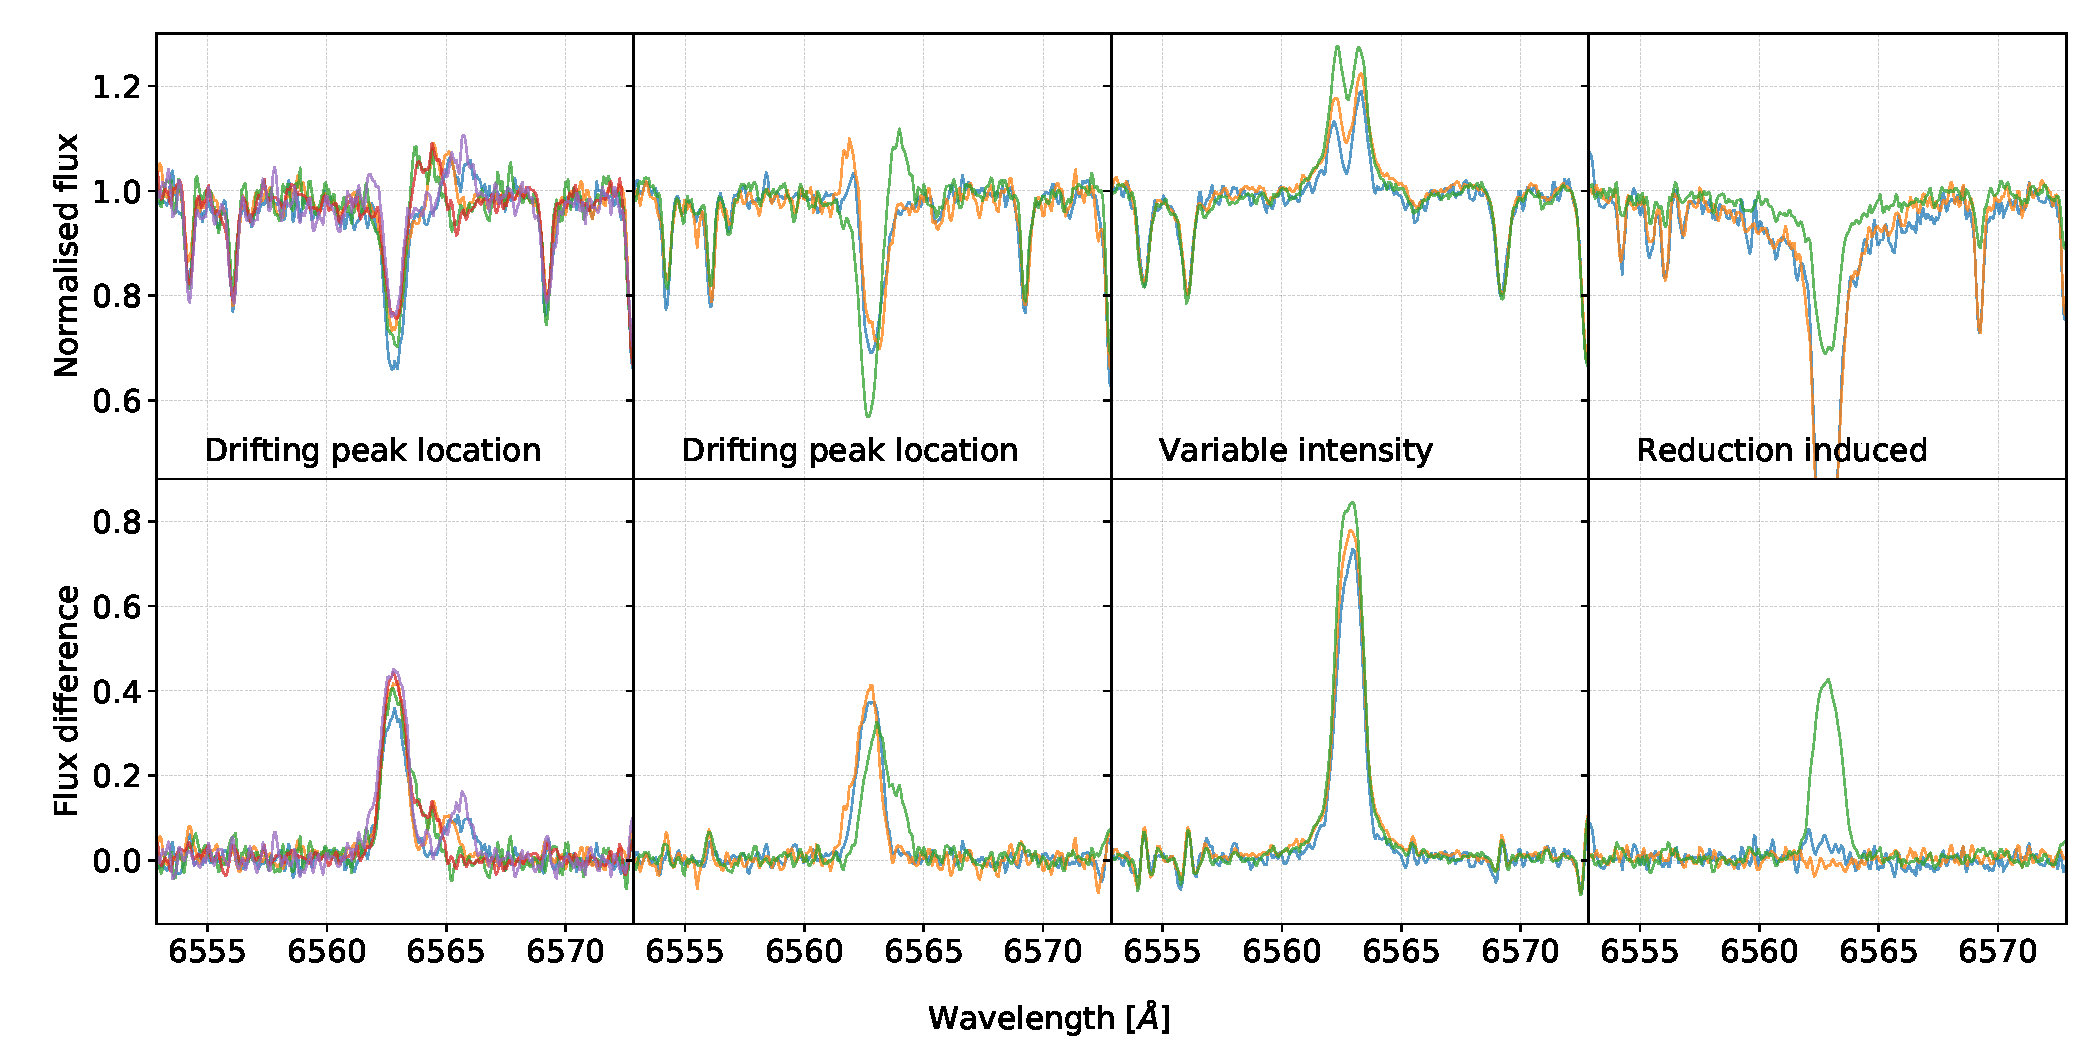
\includegraphics[width=\textwidth]{repetas_spectra_spectra_ccd3.pdf}
	\caption{A sample of objects with repeated observations, where at least one of the normalised spectra (top row) contains strong H$\alpha$ emission detected by comparison towards reference spectrum (bottom row). The first two objects (or columns) show shifting location of an additional emission component peak, and the last two varying degree of its strength. The last example is most likely a result of a miss-reduction as not only H$\alpha$, but also other absorption lines show reduced strength. The existence of this problem is confirmed by other objects in the same field as majority of them show the same tendency of having weaker absorption lines across the spectrum.} % TODO datum te noci
	\label{fig:temporal_variab}
\end{figure}

\section{Discussion and conclusions}
\label{sec:discussion_emis} 
In this chapter, we describe the development and application of a neural network autoencoder structure that is able to extract the most relevant latent features from the spectrum. Low feature dimensionality contains only the most basic spectral informations that are used to reconstruct a non-peculiar spectrum with the same physical parameters as the input spectrum.

\begin{figure}
	\centering
	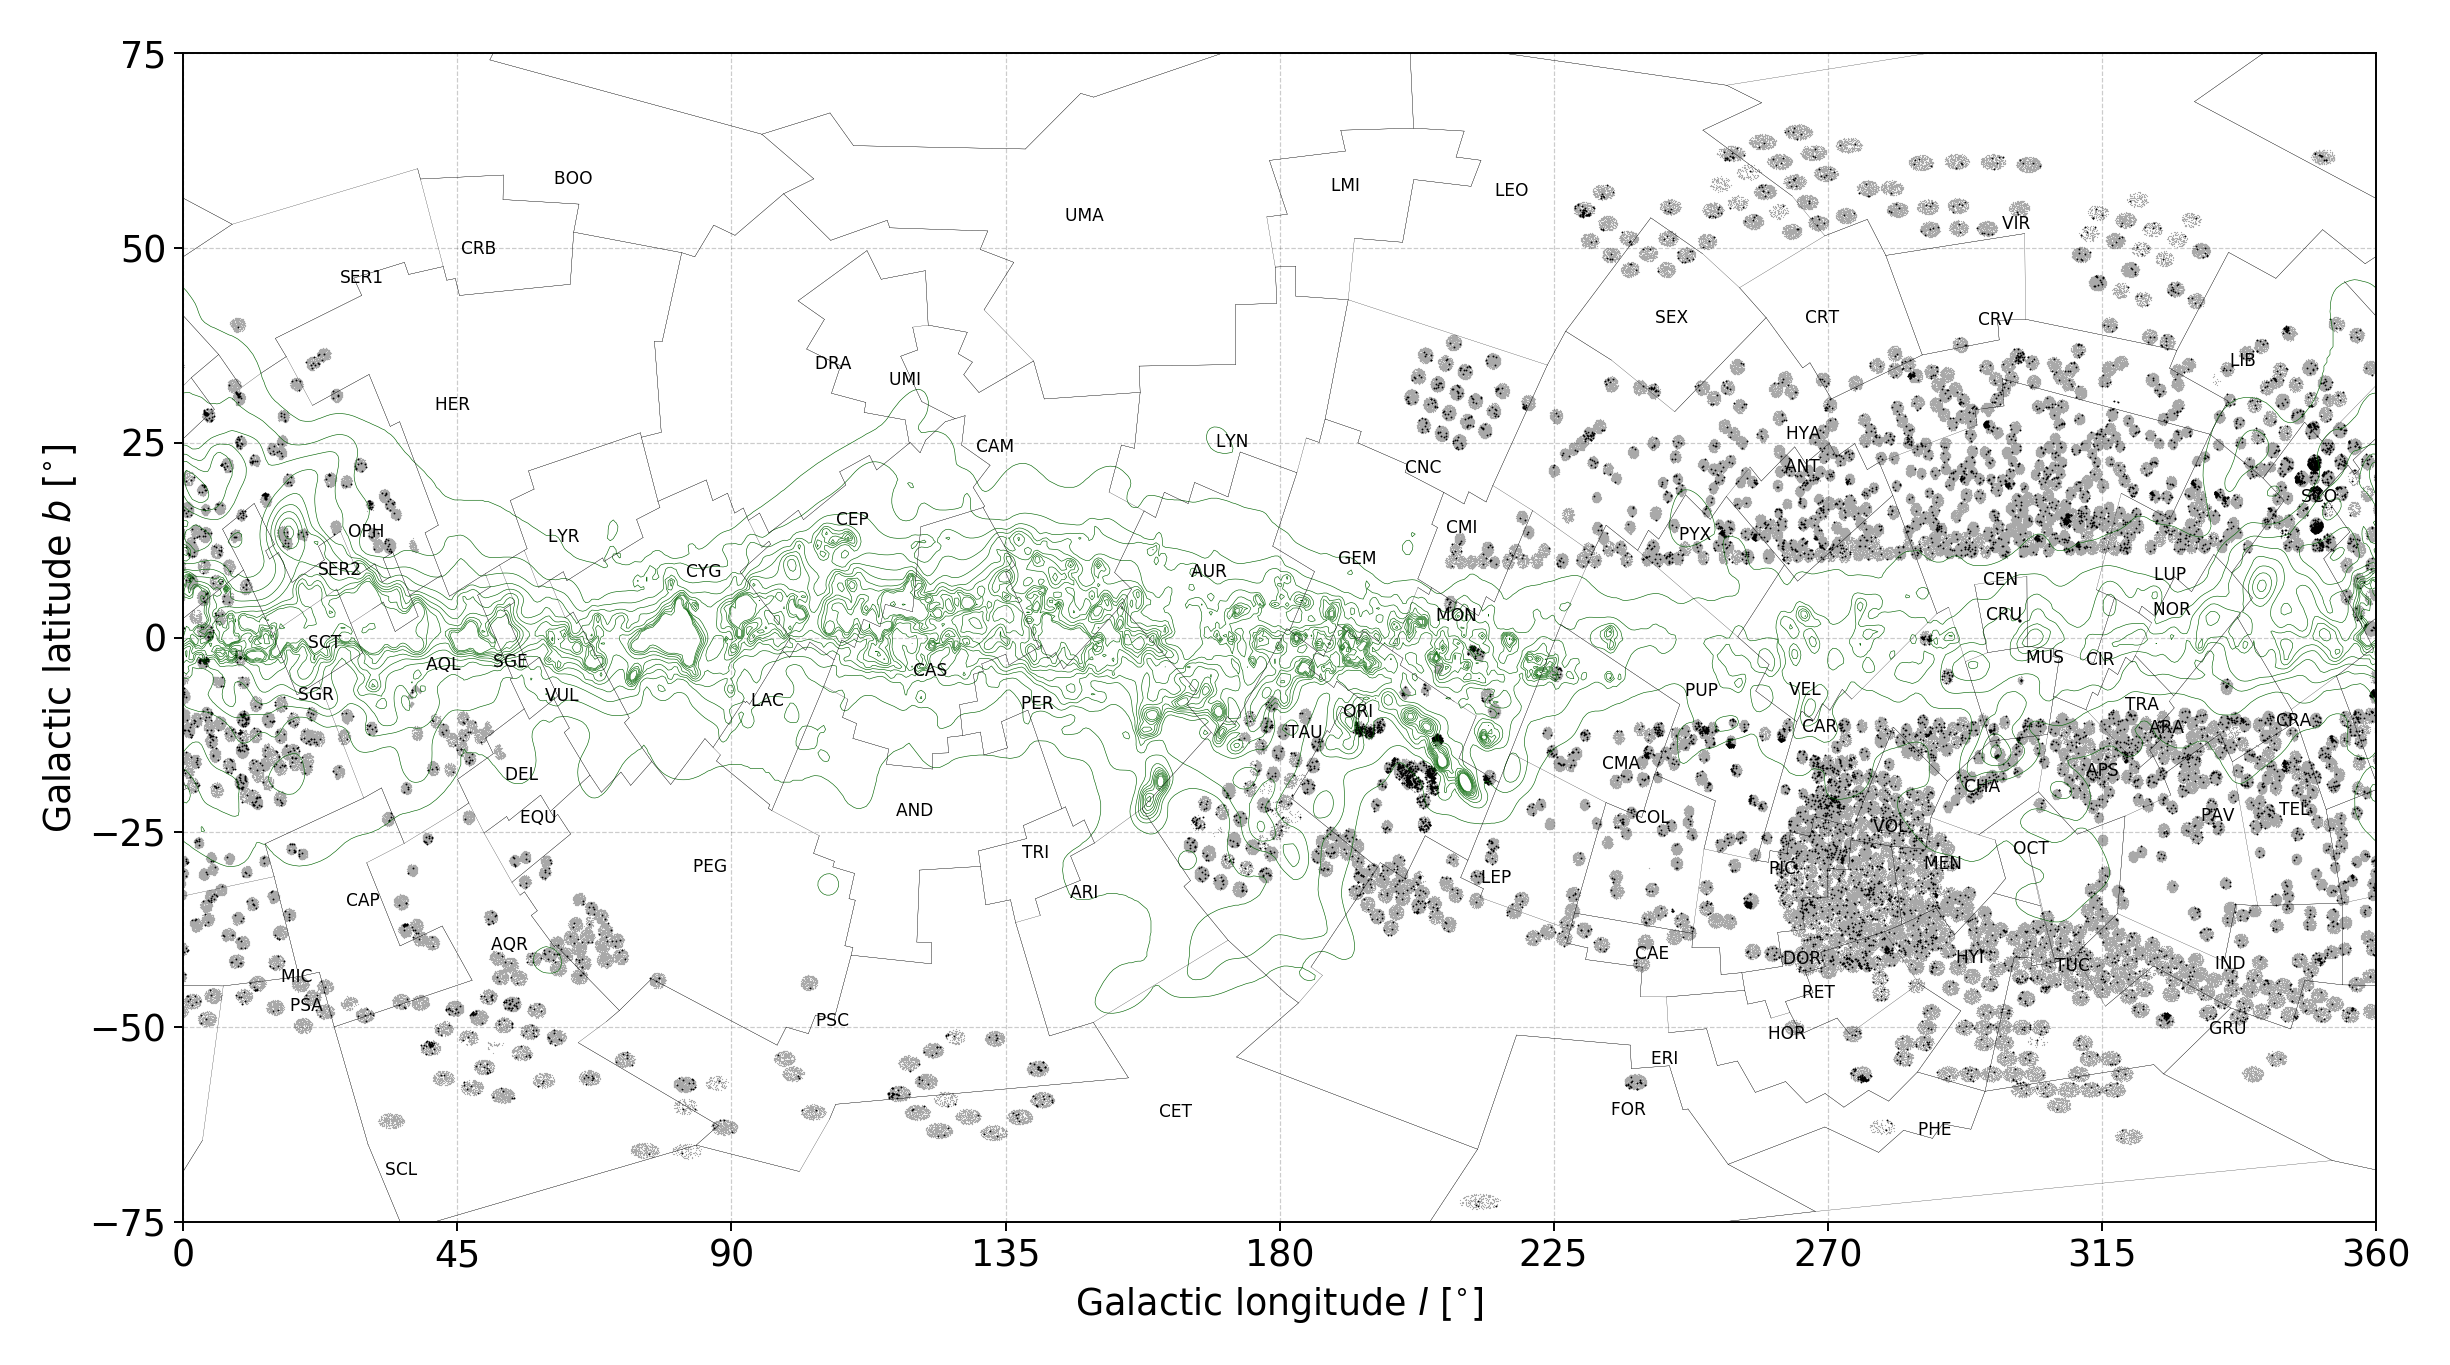
\includegraphics[width=\textwidth]{reddening_d2000_n720_cont_wemisions.png}
	\caption{Spatial distribution of stars with detected Balmer emission profiles. Grey areas represent regions that were observed and analysed in this chapter. The green lines represent location of equal reddening in steps of $0.1$ magnitude at the distance of $2$~kpc. Reddening data were taken from results published by \citet{2017A&A...606A..65C}. For readability, no isoline is shown above the reddening of 1~magnitude. Constellation boundaries were taken from \citet{const_data}. Locations of their designations are defined by median values of constellation polygon vertices.}
	\label{fig:spatialemission}
\end{figure}
% TODO Morda bi bralca spomnil, koliko je teh emisijskih zvezd in da so s črnimi simboli (neemisijske pa s sivimi, če prav razumem). Je pa sliko relativno težko brat - morda ima tu (in pri naslednji) za pozitivne detekcije bolje izbrat drugo barvo (recimo rdečo ali modro). A bi se dalo kaj tudi rečt o deležu objektov z emisijami predvsem glede na parametre (če recimo vzameš mediano parametrov, kot jih imajo zvezde z bližnjimi vrednostmi tvojih latent features). To je dodatno delo, torej premisli, koliko gre. Lažje kot ukvarjanje z latent parametri je pogledat, ali se kaj vidi glede lokacij objektov v HR diagramu (iz reddeninga na določeni razdalji (recimo Green et al.) dobiš absolutno G magnitudo in dereddened Bp-Rp barvo - takopotem lahko vsaj okvirno rečeš, za kakšne emisijske objekte gre. S pozicijami si že utemeljil, da gre za mlade objekte. Sedaj pa bo ven prišlo še kaj okrog mas: so to masivne modre zvezde ali mlade nizkomasivne, ki se šele usedajo na glavno vejo? V tekstu potem dodaš kak odstavek komentarjev na to temo. 

Our method of differential spectroscopy is one of the most widely used approaches to find peculiar spectral features that are not found in normal stars. As a part of this chapter, we showed that a dense autoencoder neural network structure can be reliably used for generation of non-peculiar reference spectra if trained on a large set of normal spectra. With the additional exclusion of our detected emission-line stars, the training set could iteratively be further cleaned of peculiar stars before training the network. As all the information about the spectral look is contained in the real flux values, there is no need to add additional convolutional layers for the extraction of more complex spectral shapes. 

By identifying significant residuals after subtracting the generated reference spectra from the observed spectra, we detected emission star candidates in the GALAH fields all over the sky. Figure \ref{fig:spatialemission} shows that we can identify few locations with a higher density of detected emission-line objects. The position of emission-line objects coincides with regions of young stars such as the Orion complex, Blanco 1, Pleiades, and other possibly random over-densities of interstellar gas and dust. Detected nebular emission in stellar spectra, shown in Figure \ref{fig:spatialnebular}, coincide with large visually-identified nebular clouds (by comparing detected locations with the red all-sky photographic composite of The Second Digitized Sky Survey, described by \citet{2000ASPC..216..145M}) such as the Antares Emission nebulae, clouds around $\pi$ Sco and $\delta$ Sco, Barnard's loop, Carina Nebula, nebulae around $\lambda$ Ori, nebular veils in the constellations of Puppis, Pyxis and Antlia, and other less prominent features.

\begin{figure}
	\centering
	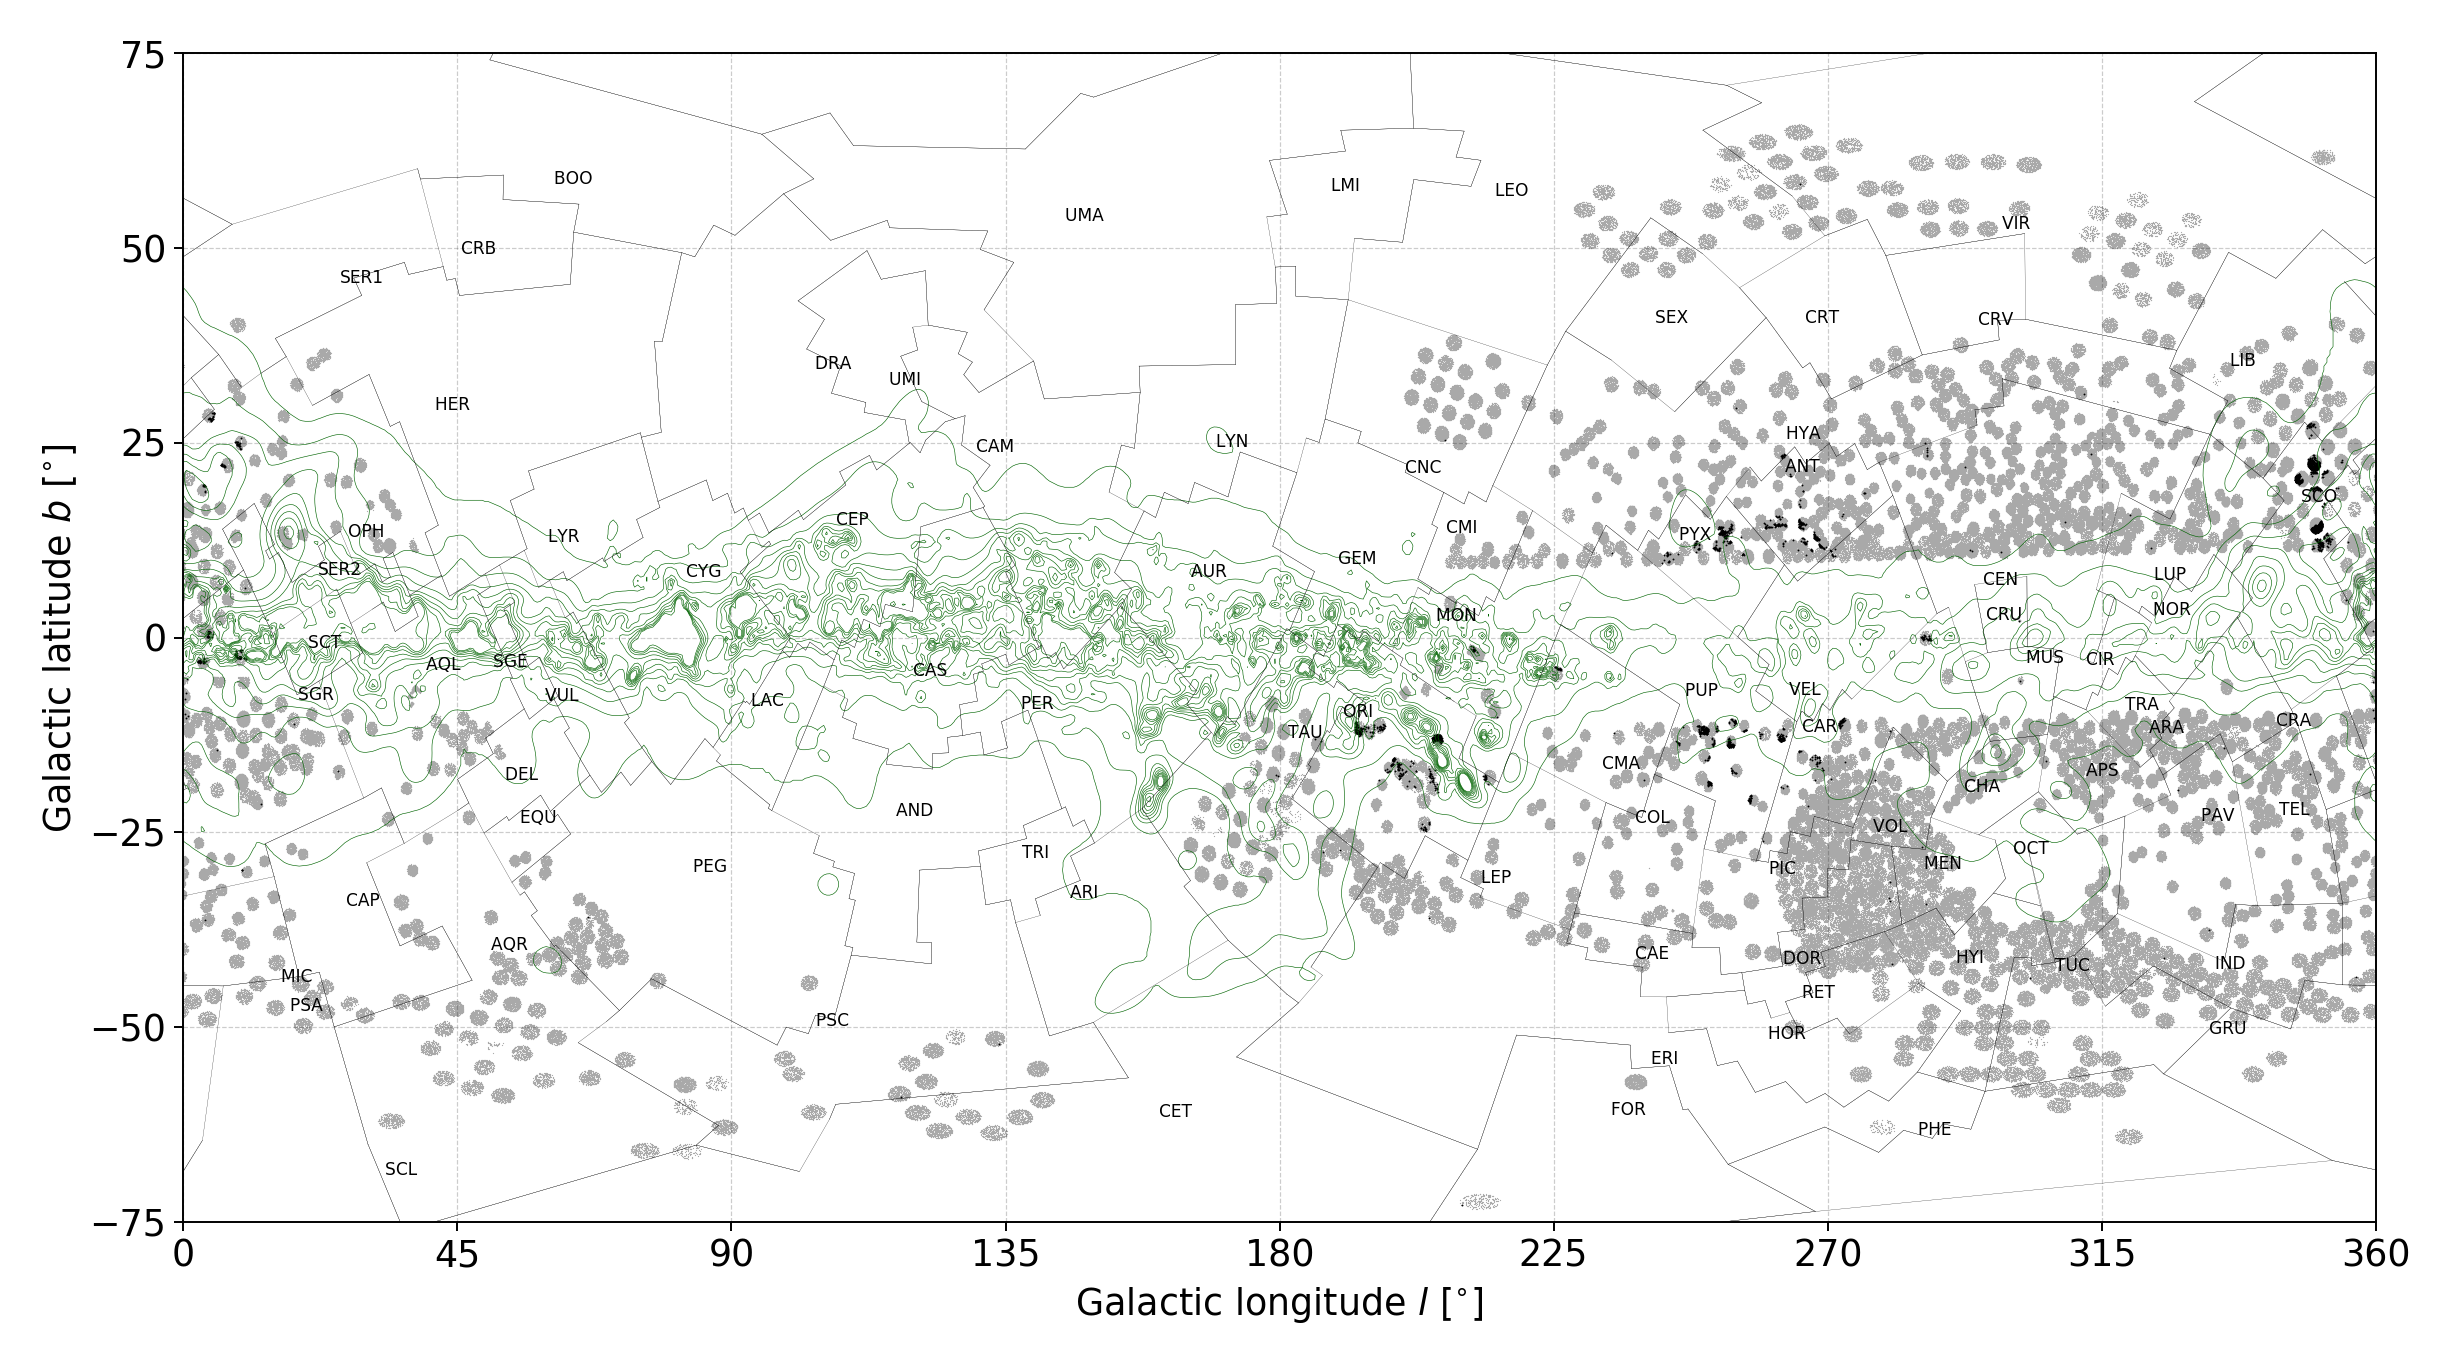
\includegraphics[width=\textwidth]{reddening_d2000_n720_cont_wnebular.png}
	\caption{Same as Figure \ref{fig:spatialnebular} but showing stars with at least three detected nebula emission lines, shown with black dots.}
	\label{fig:spatialnebular}
\end{figure}

By combining our detections with additional auxiliary data sets, we can start exploring more detailed physical explanations of the observed emissions and their structure. Among them are two specific photometric surveys, VPHAS \cite{2014MNRAS.440.2036D} and IPHAS \cite{2008MNRAS.384.1277W} which were designed to detect and study emission-line sources close to the Galactic plane. Because of their positional selection function, their combined photometric data are available only for $4431$ GALAH spectra. Of these, the spectroscopically confirmed emission stars are shown in Figure \ref{fig:iphas_vphas}, whose color-color diagram can be used to infer accreting objects.

% TODO A se da tu na nivoju enega stavka dodat, zakaj so akrecijski objekti levo zgoraj od tiste črte. In morda, kaj bi znali biti vsi ti ostali objekti (glej komentar o Gabs vs. Bp-Rp pri prejšnjem grafu). 

\begin{figure}
	\centering
	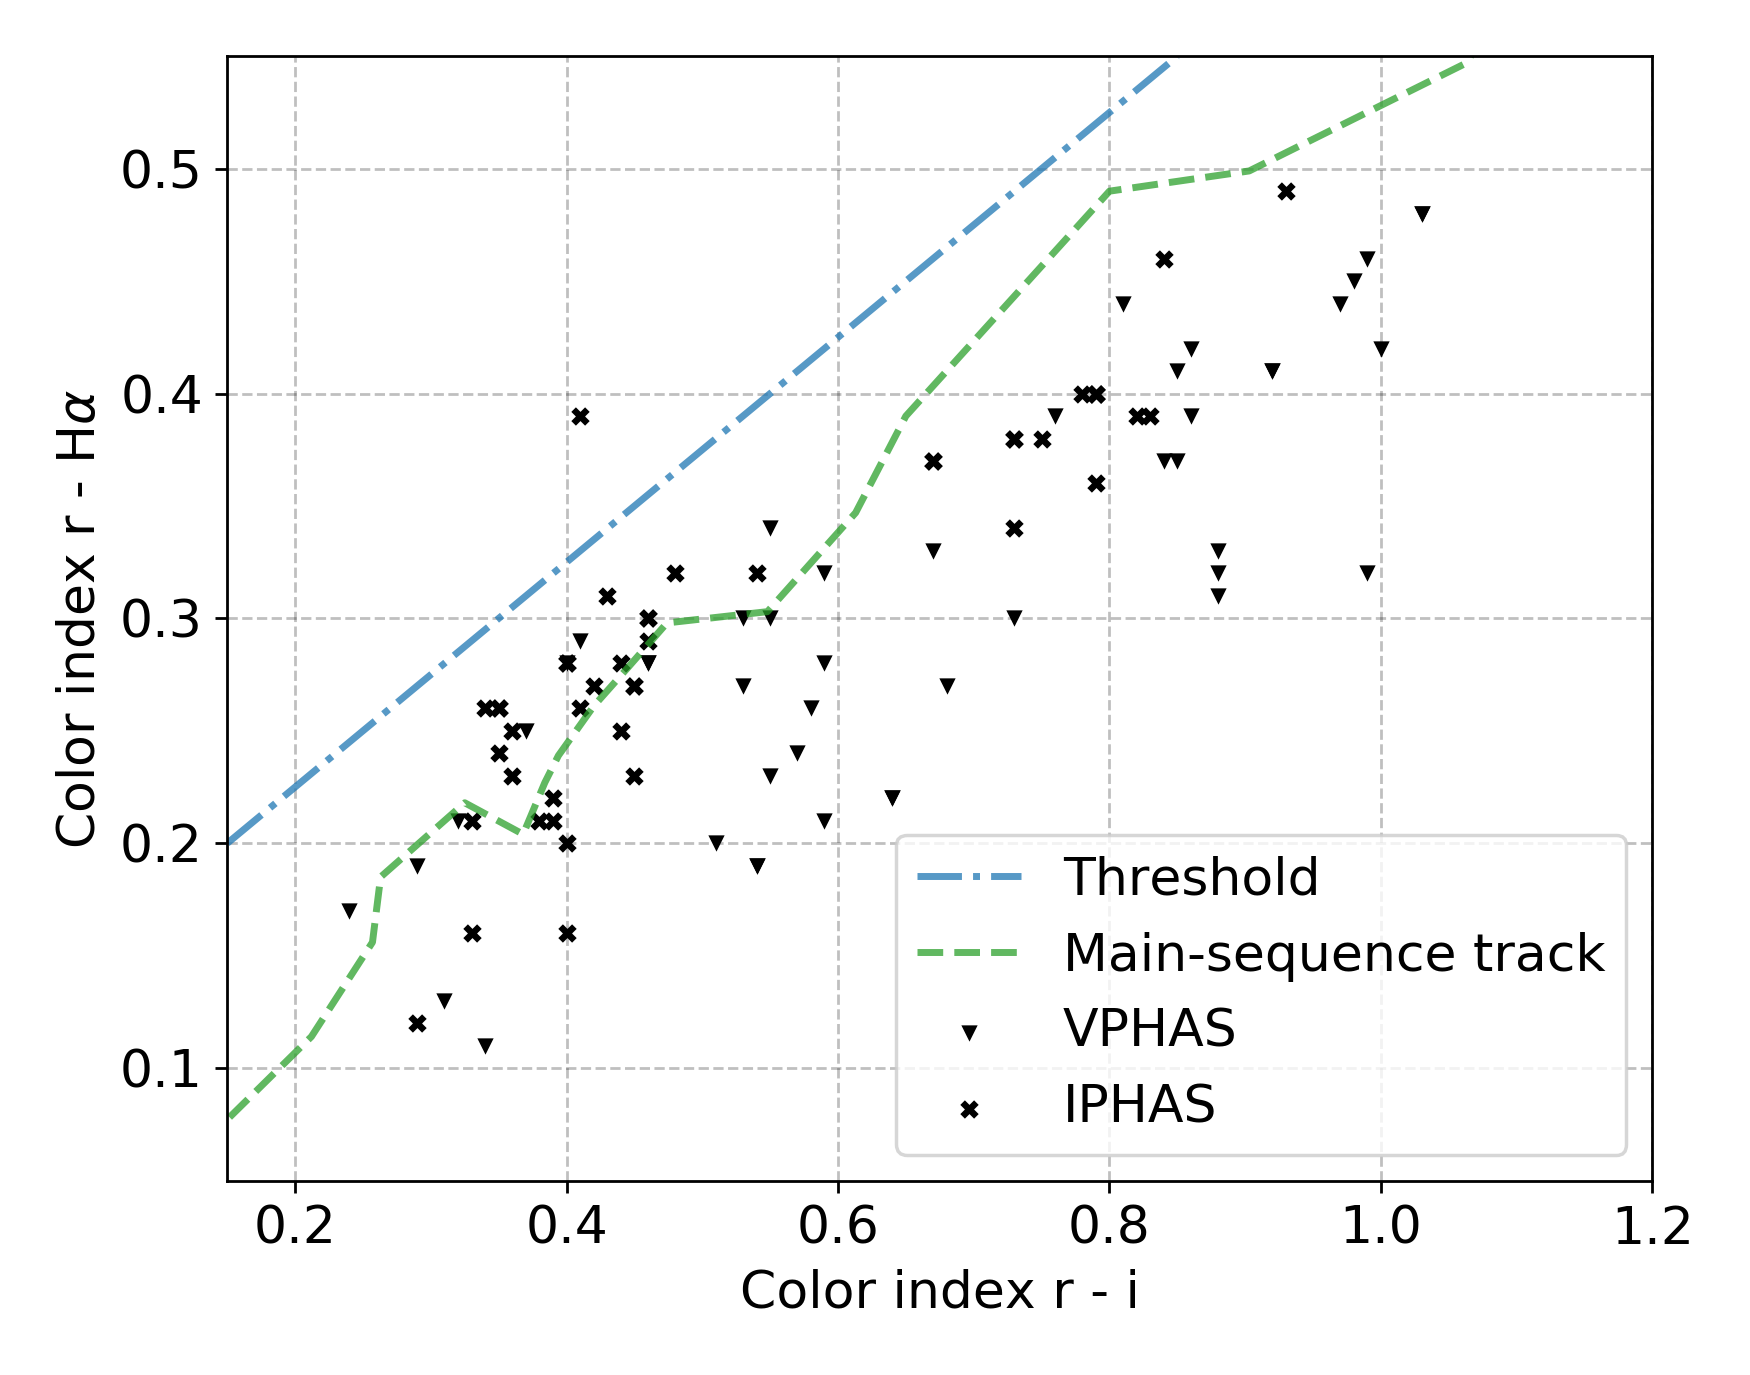
\includegraphics[width=0.6\textwidth]{mag_iphas_vphas_sep.png}
	\caption{r - H$\alpha$ versus r - i color-color diagram using combined IPHAS and VPHAS photometry for detected emission stars. The dashed green line represents the unreddened main-sequence track tabulated by \citet{2014MNRAS.440.2036D}. An empirical threshold, shown by dash-dotted blue line, can be used to distinguish non-accreting and accreting objects above the line \cite{2018A&A...609A..10V}.}
	\label{fig:iphas_vphas}
\end{figure}

Our detected emission spectra have a broad range of emission components - these range from very strong to barely detectable chromospheric emission component whose identification can be mimicked or masked at multiple steps of the analysis and data preparation. To limit the number of false-positive classifications due to reduction and analysis limitations, we focused on stronger components (\texttt{Ha\_EW}~>~$0.25$~\AA) whose existence can be confirmed visually. Because that kind of process would be slow for the whole sample, we introduced quality flags that can be used to filter out unwanted or specific cases. Additionally, the stability of the spectra and emission features was investigated by repeated observations of the same objects. Among them, we observed different variability types, of which one could be attributed to the data reduction pipeline, limiting the confidence of finding weak emission profiles in the spectra.

To reliably detect even the weakest chromospheric emissions, uncertainty of the used reference spectra must be well known as well. By showing that the proposed neural network structure can be used as intended, we are looking into possibilities to improve our methodology using variational autoencoder. Its advantage lies in the possibility of simultaneous determination of a reference spectrum and its uncertainty which would enable uncertainty estimation of the measured emission-line indices.

% TODO Nekam v te conclusions bi dodal povzetek, približno koliko emisijskih objektov si našel, približno za kakšen tip emisije gre (morfološko - npr. koliko je (a)simetričnih, koliko močnih/šibkih emisij - in tudi fizikalno (imaš že nekaj o starosti, dodaš še kaj o barvah in izsevih)).   


\chapter{Peculiar solar-like multiple stars}
\label{chap:twins}
This chapter has been partially adapted from the published paper titled \textit{The GALAH survey: unresolved triple Sun-like stars discovered by the \G\ mission} \citep{2019MNRAS.487.2474C} that was prepared and written by the author of this Doctoral thesis. The used computer code was published on GitHub platform  \footnote{\url{https://github.com/kcotar/GALAH-survey-Solar-like-triple-stars}} and results of the analysis as a catalogue on VizieR service  \footnote{\url{http://vizier.u-strasbg.fr/viz-bin/VizieR?-source=J/MNRAS/487/2474}}.

% ----------------------------------
% intro to solar twins and their spectra
% ----------------------------------

\section{Introduction}
The Sun, begin the closest and most analyzed star is widely used as a reference for the calibration of many fundamental stellar astronomical parameters \cite{2010A&A...522A..98M, 2012MNRAS.426..484D}. This implies a desire to find and catalogues as many stars similar to Sun as possible. They can be used for intra-calibration of observations done with the same setup or inter-calibration between multiple surveys that share observations of the same objects. Stars resembling the Sun in all physical parameters such as luminosity, mass, radius, rotation period, and chemical composition should also have an identical spectrum like our Sun. The definition of such stars, also known as solar twins, was first introduced by \citet{1981A&A....94....1C}, but it is still far from being finalized as it follows evolution of astronomical instrumentation, observational techniques \cite{2017AN....338..442A}, and quality of determined stellar parameters and chemical abundances.

Before the release of accurate parallaxes, nowadays measured by the \G\ satellite, one of the approaches to determine distances of twin stars or its hosting stellar cluster was based on the assumption that solar twins should have the same intrinsic luminosity as the Sun. Therefore its apparent brightness on the sky is directly related to its distance \cite{2015MNRAS.453.1428J, 2016A&A...595A..59M, 2017MNRAS.472.2517J}.

Another widely debated topic is the chemical composition of the Sun and its evolution in time. \citet{2009A&A...508L..17R, 2015A&A...579A..52N} addressed the question if the composition of the Sun is peculiar when compared to other solar twins. Works like these benefit from using spectra with high signal to noise ratio and very high spectral resolution that are especially needed when trying to disentangle if the observed solar chemical composition is a consequence of the planetary system formation \cite{2014A&A...572A..48R} or intrinsic galactic chemical composition during formation of the Sun \cite{2015A&A...579A..52N, 2016A&A...593A..65N, 2020A&A...633L...9J}. However, even the best solar twin candidates (currently tough to be the star 18 Sco \cite{2014ApJ...791...14M}), when observed with the highest possible precision, still show minute differences in the abundance pattern which will make it even harder to disentangle the place where the Sun and its siblings were formed.

% With the increasing number of large all sky surveys, searches for the closest solar twin have been performed on numerous on-going and archival data sets. 

\section{Selection of the best solar-like spectra}
\label{sec:05_selection}
Our search for spectra that most resemble spectrum of the Sun uses data acquired by the GALAH survey and few other surveys that used the same telescope and spectrograph. The search is based on the direct comparison between a random acquired stellar spectrum and the reference solar spectrum, where both were observed with the same setup of the HERMES spectrograph.

\subsection{Reference Solar spectrum}
\label{sec:05_reference}
Before finding the best solar-like spectra in our data set, the reference spectrum had to be constructed. For its construction, we identified $3708$ twilight flats with the SNR per resolution element in the green HERMES arm greater than 210. Selected spectra were first normalised using the $7^\text{th}$ degree Chebyshev polynomial with an asymmetric sigma clipping ($2\sigma$ low and $3\sigma$ high threshold) that was run for $11$ steps. Normalisation procedure was tailored explicitly for solar-like objects as it excluded wavelength ranges with wide absorption features and regions with no near continuum levels that were determined from the high-resolution spectrum of the Sun created by \citet{2005MSAIS...8..189K}. Especially problematic for the normalisation process is the blue arm that is packed with absorption lines, topped by the H$\beta$ line. Because of high SNR and presence of additional "wiggles" in observed twilight flats, we used a higher degree of polynomial function than in the case of a stellar spectrum normalisation (see Section \ref{sec:05_preprocessing}). Source of identified additional spectra features is not known and might be contributed by a reflection in optics when observing bright targets or by a residual background flux that was not properly removed by the GALAH reduction pipeline \cite{2017MNRAS.464.1259K}

The radial velocity of normalised twilight spectra was determined by correlating an observed spectrum with the high-resolution solar spectrum \cite{2005MSAIS...8..189K}. The peak of the resulting correlation function was determined by fitting the Gaussian function to it. Before correlation, the high-resolution solar spectrum was convolved with a Gaussian kernel to match its resolving power with the HERMES spectrograph and to visually look as close as observed spectra as possible. 

Normalised twilight spectra, shifted to the rest-frame, were then median stacked to generate the final reference solar spectrum. Before it could be used, it was analyzed for possible residual flux offsets that are impossible to remove by the reduction pipeline as we can not acquire background spectrum at the same time as a twilight spectrum. Any residual flux would render too shallow absorption lines in the median reference Solar spectrum. To equalize strengths of absorption lines in our reference Solar spectrum and the high-resolution one, a small linearly changing offset was subtracted from the normalised spectrum that was re-normalised after subtraction. 

\subsection{Stellar spectra preprocessing}
\label{sec:05_preprocessing}
Preprocessing of observed stellar spectra began with combined and fluxed spectra that were prepared by the pipeline as an intermediate reduction result. Firstly they were normalised using $5^\text{th}$ degree Chebyshev polynomial and asymmetric sigma clipping ($2\sigma$ low and $3\sigma$ high threshold) that was run for $15$ steps. To determine the level of a continuum as accurately as possible, we masked spectral ranges without near continuum pixels (H$\alpha$ and H$\beta$) during the normalisation process. Normalised spectra were then shifted for the barycentric and radial velocity that was determined by the GALAH pipeline and linearly resampled to the same wavelength step as used by the generated reference solar spectrum. Performing both steps (radial velocity shift and resampling) at the same time retain a quality of the spectrum and reduces the number of resampling steps compared to if we would use already shifted and normalised spectra prepared by the pipeline.

\subsection{Candidate selection}
\label{sec:05_candidates}
As the number of spectra in our set is quite large (more than $600,000$) and some of them have entirely different spectrum than the Sun (e.g. hot stars, metal-poor giants, cool stars), we performed an initial selection of possible solar twins purely based on stellar physical parameters. They were determined by \TC\ interpolation pipeline \cite{buder2018}, that was part of the GALAH data release 2. For this, we first had to determine the possible offset of our interpolated parameters towards the parameters of well known solar-like benchmark stars \cite{2014A&A...564A.133J, 2015A&A...582A..49H} and the Sun. Offset determination was done by comparing parameters of well-studied stars that were observed by the GALAH survey. Table \ref{tab:params_twins} gives reference values of physical parameters for the Sun alongside median parameters of selected twilight flats and their standard deviations. 

\begin{table}
	\centering
	\caption{Stellar physical parameters of reference objects used to determine possible offsets between published benchmark values and values determined by \TC. For every object, the first line in table gives reference values and the second line parameters determined from the GALAH spectra.}
	\label{tab:params_twins}
	\begin{tabular}{r c c c}
		\hline
		Object & \Teff\ [K] & \Logg\ [dex] & \Feh\ [dex] \\ 
		\hline
		Sun & $5771$ & $4.44$ & $0.02$ \\ 
		Flats & $5605 \pm 40$ & $4.21 \pm 0.06$ & $-0.14 \pm 0.03$ \\ 
		\hline
		18 Sco & $5810 \pm 80$ & $4.44 \pm 0.03$ & $0.03 \pm 0.01$ \\
		& $5750 \pm 20 $ & $4.37 \pm 0.1$ & $ 0.05 \pm 0.02$ \\ 
		\hline
		$\beta$ Hyi & $5873 \pm 45$ & $3.98 \pm 0.02$ & $-0.04 \pm 0.01$ \\
		& $5784 \pm 5$ & $3.93 \pm 0.01$ & $-0.11 \pm 0.01$ \\ 
		\hline
		$\mu$ Ara & $5902 \pm 66$ & $4.3 \pm 0.03$ & $0.35 \pm 0.01$ \\
		& $5657 \pm 20$ & $4.15 \pm 0.01$ & $0.28 \pm 0.01$ \\
		\hline
	\end{tabular}
\end{table}

Table \ref{tab:sim_combine_twins} also shows parameters for three benchmark stars with Solar like properties that were observed and reduced as any other object in our data set. Parameter values in the first line were taken from the published set of \G\ FGK benchmark stars (\cite{2014A&A...564A.133J, 2015A&A...582A..49H}) and the second line gives \TC\ parameters for the same object. From the comparison it is obvious that twilight flats have slightly more under-determined parameters as apposed to other stars used in the comparison. \TC\ trend, of stellar parameters being a bit too low, is observable for all stars and parameters given in the Table \ref{tab:params}. Taking this into consideration, we initially selected stars a within broader range of \Teff$ \pm 250 $~K, \Logg$ \pm 0.4 $~dex and \Feh$ \pm 0.3 $~dex around median parameters of twilight flats. Applying parameter cuts to our data set, we were left with 92284 spectra that were analyzed further.

\subsection{Spectral similarity}
\label{sec:spec_comp_twins}

\begin{figure}
	\centering
	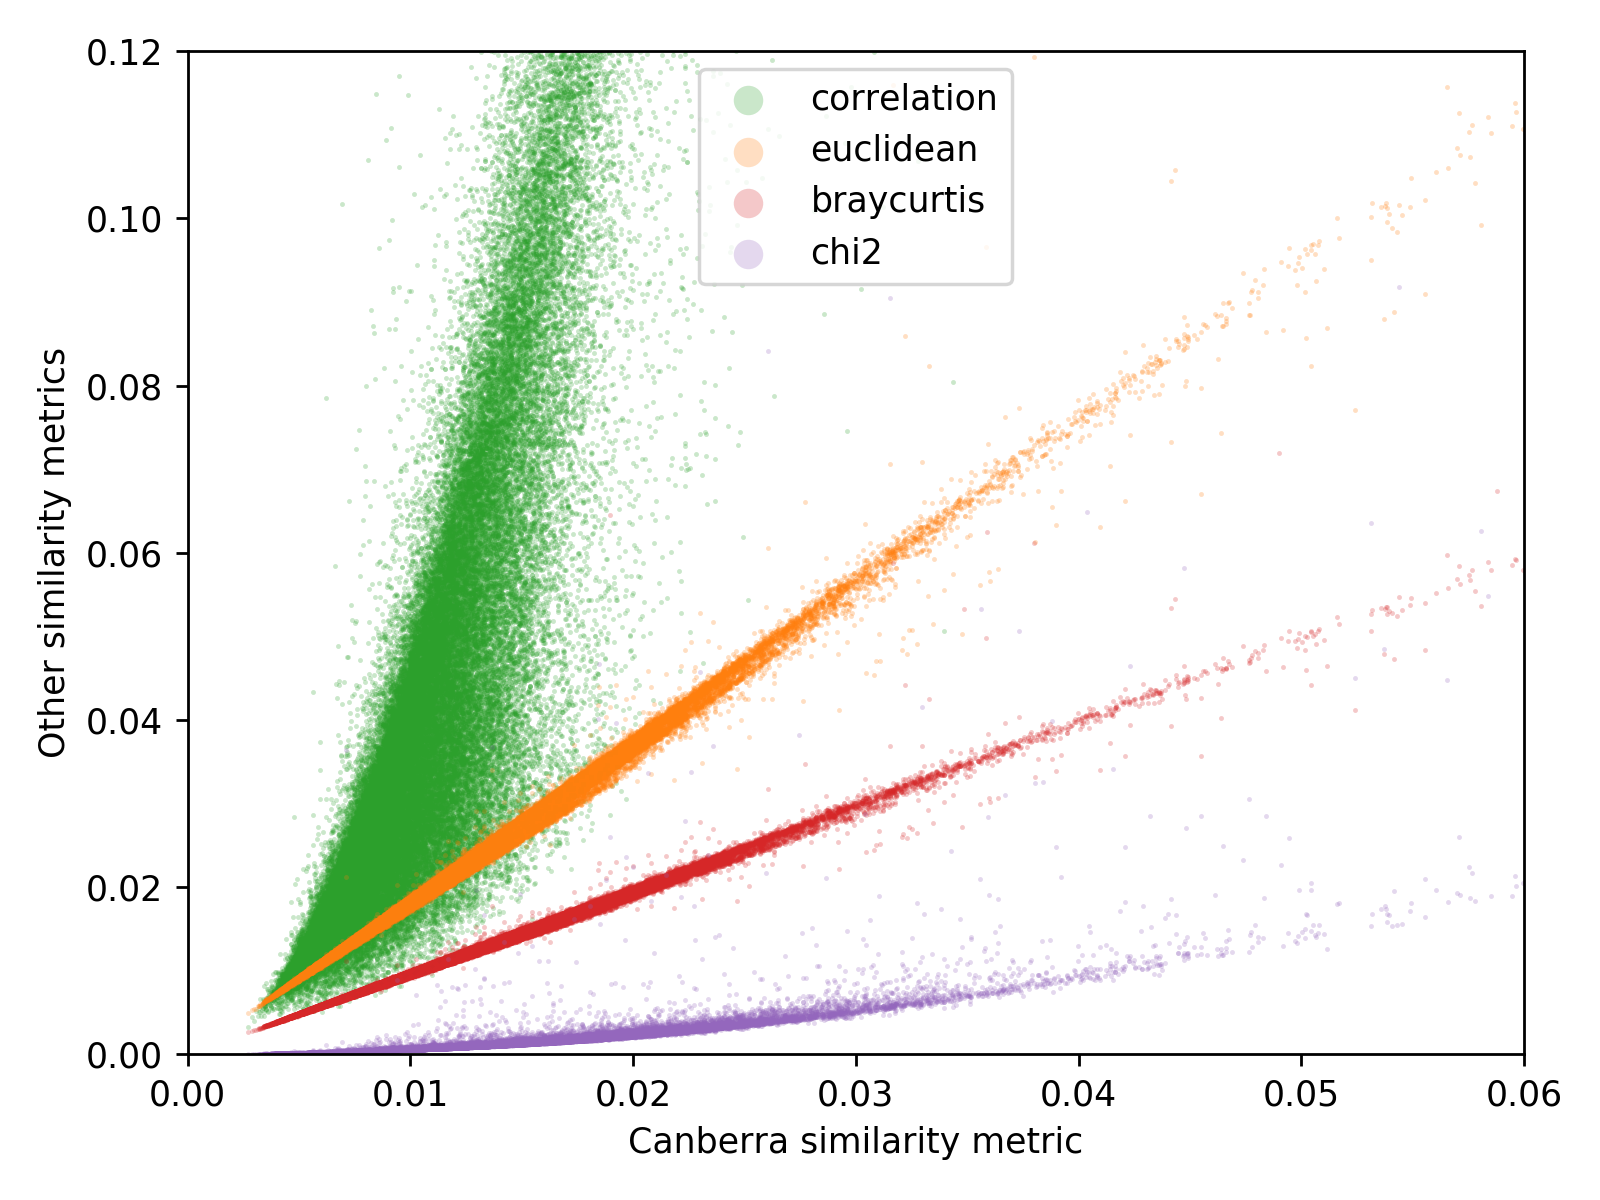
\includegraphics[width=0.75\textwidth]{sim_combine_b2.png}
	\caption{Correlation between different similarity metrics for the objects considered in the rough spectral comparison step.}
	\label{fig:sim_combine_twins}
\end{figure}

The similarity between observed spectra and generated reference solar spectrum was calculated using multiple distance metrics, where identical spectra are described by the similarity value of 0. Figure \ref{fig:sim_combine} shows that all considered metrics are strongly linearly correlated with few outliers. Some degree of the correlation was expected as all of the shown metrics are based on differently weighted per pixel difference between two spectra. For all the following comparisons we choose to use the Canberra distance metric \citep{Lance1967MixedDataCP} that is less sensitive to large, unnatural outlying flux values than the Euclidean distance and is defined as 
\begin{equation}
	\label{equ:equ_canberra}
	distance_{Canberra}(f_{\odot}, f_{obs}) = \sum_{\lambda}^{\ } \frac{|f_{\odot,\lambda} - f_{obs,\lambda}|}{|f_{\odot,\lambda}| + |f_{obs,\lambda}|},
\end{equation}
where $f_{\odot}$ is the reference solar spectrum and $f_{obs}$ an observed spectrum. Similarity value determined by the given function heavily depends on the SNR of the evaluated spectrum, which effectively degrades its spectral similarity at lower SNR values. Dependency was analysed by computing the same similarity metric between the original reference solar spectrum and noisy reference that was generated by adding noise with Gaussian distribution to the original spectrum to represent spectra with different SNR values. To determine the uncertainty of similarities, the test was repeated 1500 times for every noise level. Smooth dependence between SNR and similarity metric can be described by the following composite of linear and power-law function
\begin{equation}
	\label{equ:sim_twins}
	sim(SNR) = A \Big(\frac{SNR-SNR_{off}}{SNR_0}\Big)^{-\alpha} + B (SNR-SNR_{off}) + C,
\end{equation}
that was fitted to the resulting points shown in the Figure \ref{fig:similarity_snr_twins}. Parameters $A$, $B$, $C$, $SNR_0$, $SNR_{off}$ and $\alpha$ in Equation \ref{equ:sim_twins} are free and were fitted to the simulated similarity measurements at different SNR levels.

\begin{figure}
	\centering
	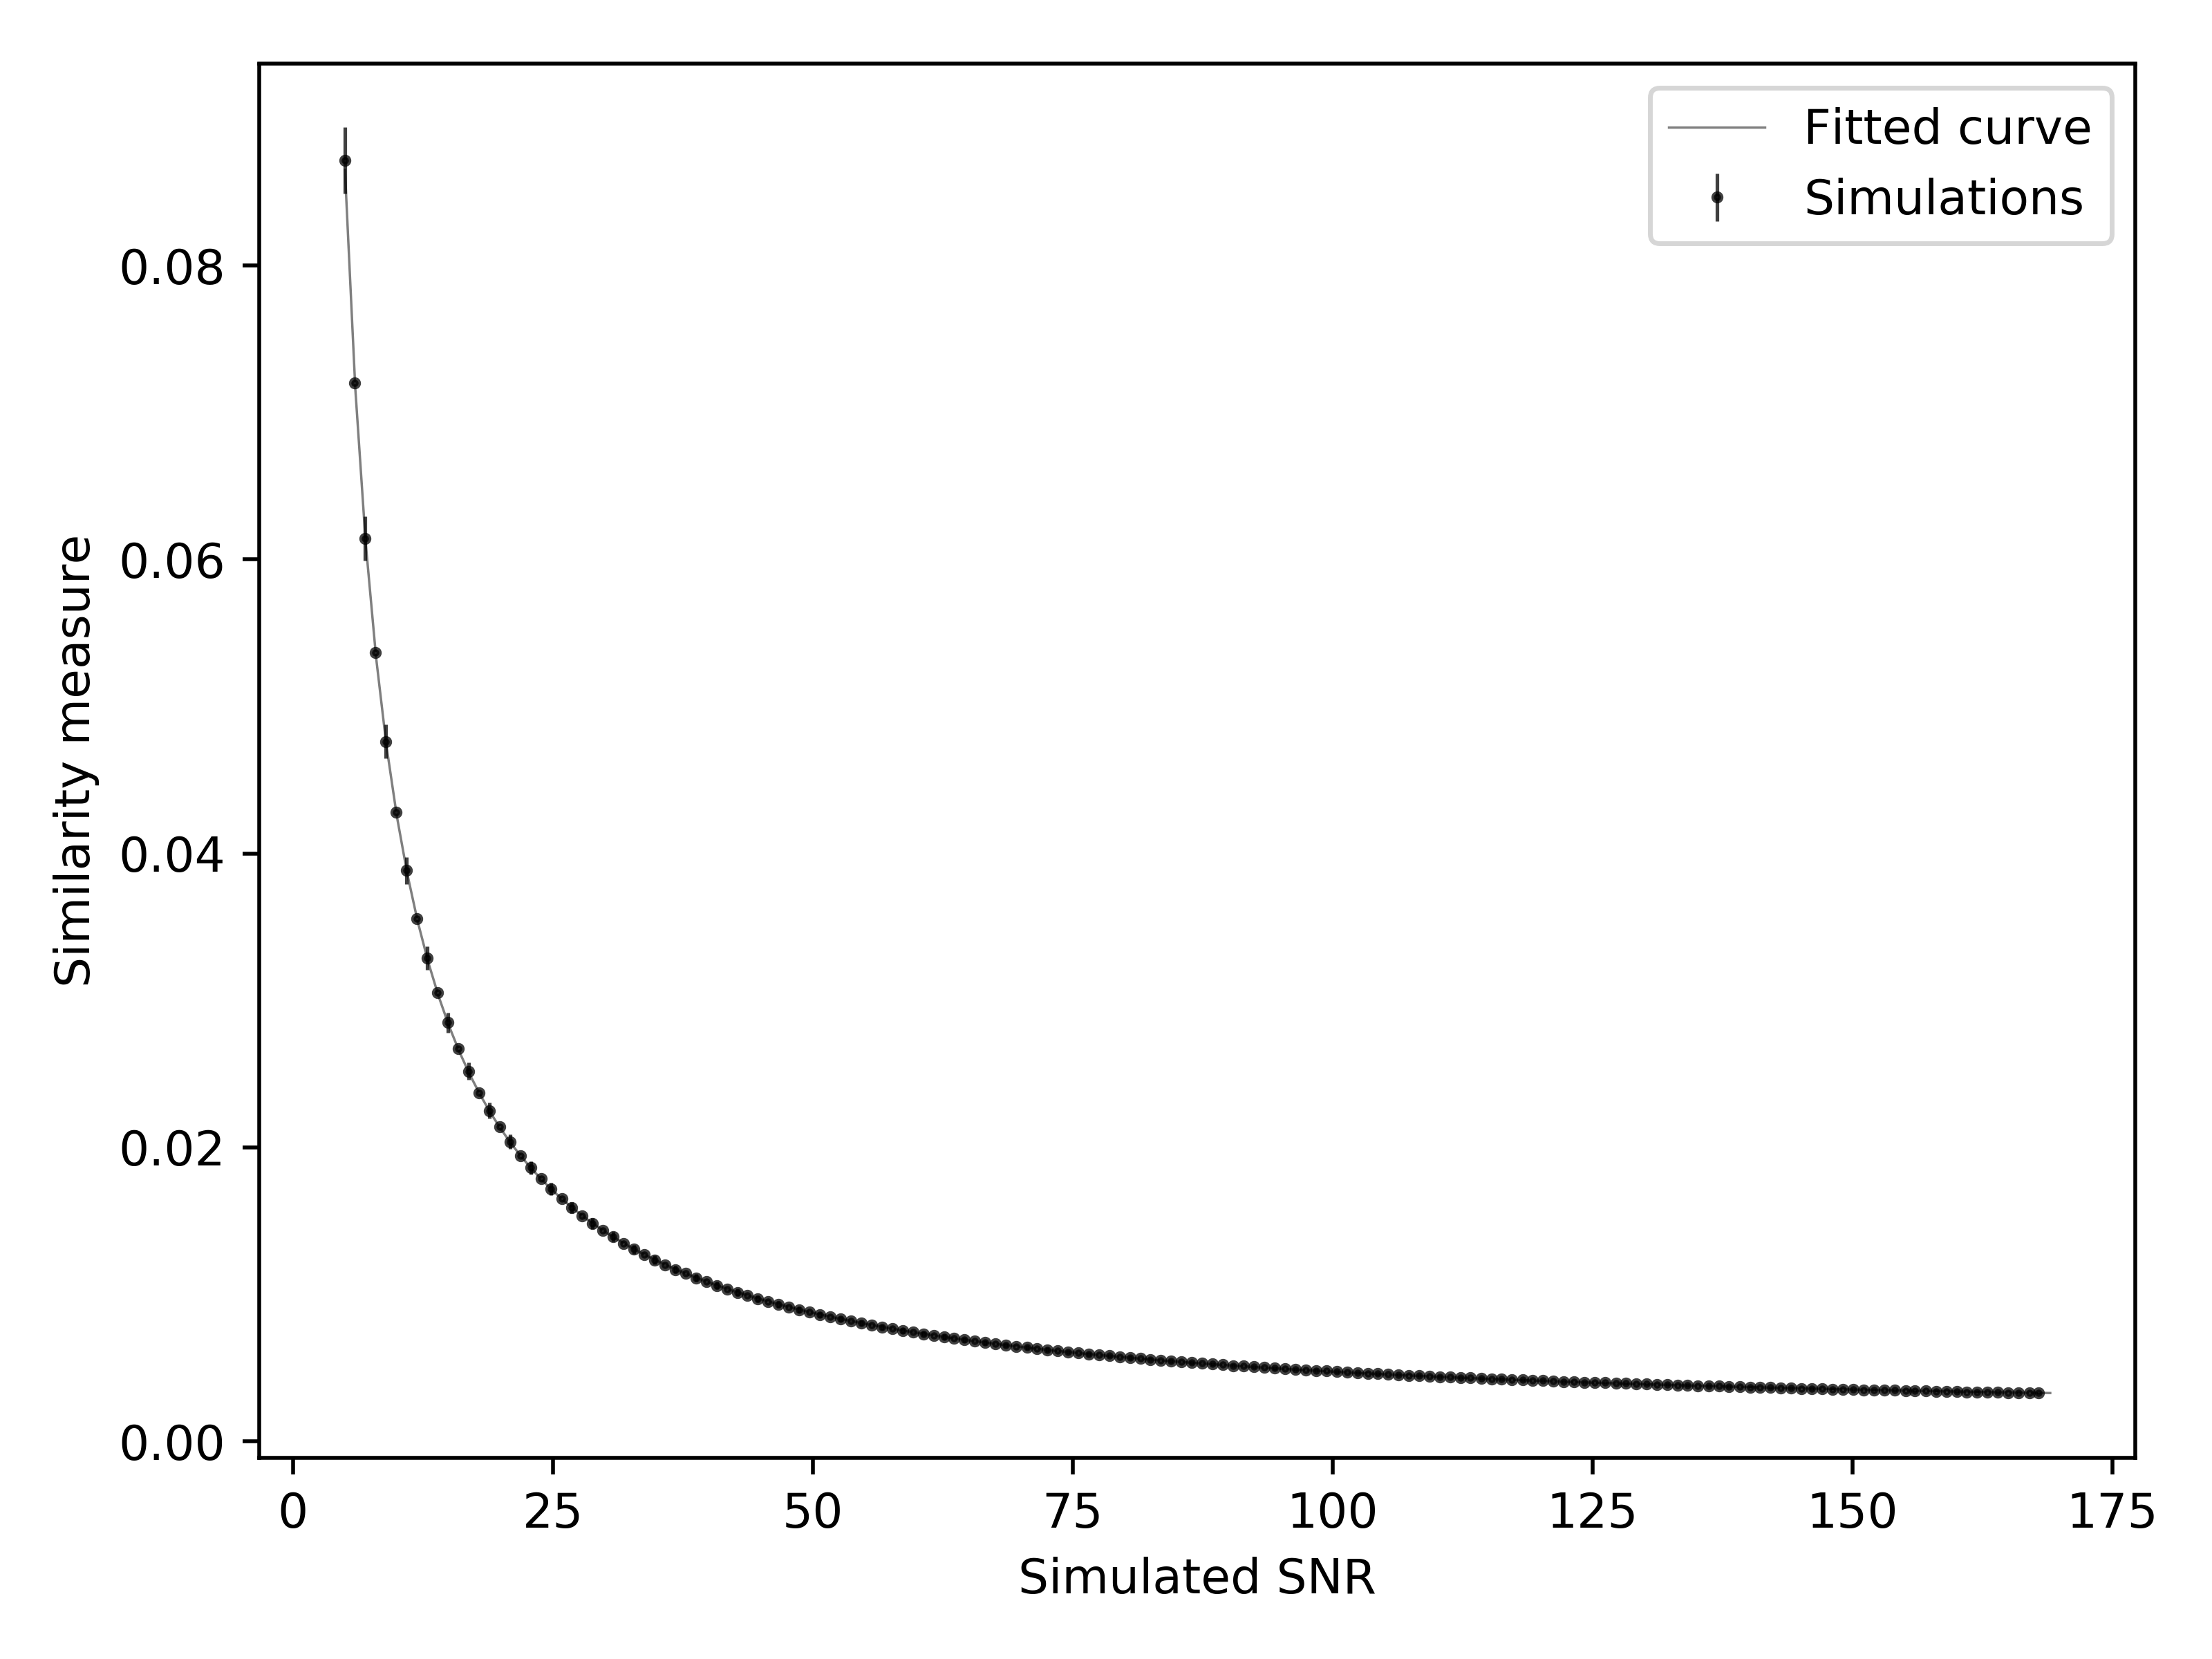
\includegraphics[width=0.75\textwidth]{canberra_b2_flux0_05.png}
	\caption{Equation \ref{equ:sim_twins} fitted to the simulated data points describing dependence between spectral SNR and Canberra distance metric of noisy solar spectrum in comparison towards the original noise free spectrum of the Sun.}
	\label{fig:similarity_snr_twins}
\end{figure}

We used the above-described similarity distance (Equation \ref{equ:equ_canberra}) to compare observed spectra along the following ranges of HERMES spectrum: 4725~-~4895~\AA\ in the blue arm, 5665~-~5865~\AA\ in the green arm, 6485~-~6725~\AA\ in the red arm and 7700~-~7875~\AA\ in the near-infrared spectral arm. Selected ranges are valid for all observed spectra. They do not pose any limitations on the number of usable spectra that might have undefined flux values at the range borders because of large radial velocities. The similarity between reference and an observed spectrum was not computed for the whole specified spectral range but was limited to known and isolated (not blended) spectral absorption lines, representing multiple different chemical elements. Their statistics are given in Table \ref{tab:elements_list} and is the same as used by \TC\ abundance determination procedure described in \citet{buder2018}. Around the central wavelength of each absorption line, wavelength pixels in the mean range of $0.47$~\AA\ are considered for the comparison. The range differs for every line and is not necessarily centred on a given line centre \cite{buder2018}.

\begin{table}
	\centering
	\caption{Number of absorption lines for different chemical elements that were used to measure similarity between observed and reference spectrum. Elements marked with * are problematic for precise abundance determination in solar twins because of their shallow or rarely noticeable absorption feature. Total number of used absorption lines is 180.}
	\begin{tabular}{l l c | c l l }
		\hline
		Element & Lines & & & Element & Lines\\ 
		\hline
		Al & 4 & & & Na & 3\\ 
		Ba & 2 & & & Nd* & 5\\ 
		C* & 1 & & & Ni & 7\\ 
		Ca & 5 & & & O & 3 \\ 
		Co* & 3 & & & Rb* & 1\\ 
		Cr & 9 & & & Ru* & 1\\ 
		Cu & 2 & & & Sc & 10\\ 
		Eu* & 2 & & & Si & 4\\ 
		Fe & 52 & & & Sm* & 2\\ 
		K* & 1 & & & Sr* & 1\\ 
		La* & 4 & & & Ti & 20\\ 
		Li* & 1 & & & V & 17\\ 
		Mg & 2 & & & Y & 4\\ 
		Mn & 4 & & & Zn & 2\\ 
		Mo* & 2 & & & Zr* & 4 \\ 
		\hline
	\end{tabular}
	\label{tab:elements_list}
\end{table}

\subsubsection{Best candidates}
\begin{figure}
	\centering
	\includegraphics[width=0.75\textwidth]{canberra_b3_07_envelope.png}
	\caption{Equation \ref{equ:sim_twins} was fitted to thresholding values, denoted with red downwards arrows, that delineated 7\% of the most similar spectra in every narrow SNR bin. The resulting fit on the thresholding values is represented by the blue dashed line. Shown plot is made for the red spectral arm.}
	\label{fig:envelope_fit_twins}
\end{figure}

The spectral comparison described in Section \ref{sec:spec_comp_twins} was independently computed for every HERMES arm. With four similarity values per spectrum, we selected the set of best matching spectra in the following way. As the similarity value heavily depends on the SNR value of a spectrum, we first determined thresholding similarity values for the best 7\% of spectra in each narrow SNR bin. The thresholds are in Figure \ref{fig:envelope_fit_twins} visualized as red downward arrows. Width of the SNR bins was set to $4$ and separation between them to 2 SNR values. After fitting the function described by Equation \ref{equ:sim_twins} to those thresholds, the best matching objects were all whose spectral similarity fell below the fitted line. By combining all four bands, we determined $329$ objects whose spectral similarities fell bellow the fitted thresholding line in all HERMES bands. Considering every spectral arm individually, we effectively removed objects with possible reduction problems in any of them. Spectra determined to be the best solar twin candidates are show in Figure \ref{fig:selection_step1_twins}.

\begin{figure}
	\centering
	\includegraphics[width=\textwidth]{selection_step1.png}
	\caption{Visual comparison between a set of the most probable solar twins spectra and the solar reference spectrum shown in black. Grayed out regions represent wavelength ranges used in the similarity computation described in Section \ref{sec:spec_comp_twins}. Chemical element responsible for the observed line is also indicated above the spectra for every absorption line.}
	\label{fig:selection_step1_twins}
\end{figure}

%\begin{figure}
%	\centering
%	\includegraphics[width=\columnwidth]{solar_twins_like_Teff_cannon.png}
%	\includegraphics[width=\columnwidth]{solar_twins_like_Logg_cannon.png}
%	\includegraphics[width=\columnwidth]{solar_twins_like_Fe_H_cannon.png}
%	\caption{Histogram of parameters \Teff, \Logg\ and \Feh\ for selected Solar twin candidates based on their spectral similarity towards the Solar reference spectrum. Red vertical line represents median value of the histogram and black line the Solar value of the same parameter.}
%	\label{fig:step1_params}
%\end{figure}

\section{Chemical composition}
\begin{figure}
	\centering
	\includegraphics[width=\textwidth]{abund_all_selection.png}
	\label{fig:abund_candidates}
	\caption{\rb{TODO ali pa tudi ne, mogoce plot s starostmi} Normalized distribution of unflaged abundance values determined by \TC\ procedure for the complete set of Solar twin candidates. Median value and one sigma deviation are marked by the red vertical lines in the plot. Values on the left represent number of used abundance values for the construction of histogram and its median deviation from zero abundance value that should represent Solar abundance after \TC\ corrects for the abundance value measured in the HERMES Solar spectra as explained by \protect\cite{buder2018}.}
\end{figure}


\section{Follow-up observation}
In order to evaluate our selection of the best candidates, we acquired multiple high-resolution Echelle spectra. Here we present the spectrum of a star TYC 502-985-1 that was one of our best candidates and is observable from the Asiago observatory located in the northern hemisphere. The acquired spectrum that spans a much wider wavelength range than the HERMES spectrum is presented in Figure \ref{fig:asiago_spectrum_twin}. The final spectrum consists of three $30$~min long exposures that were individually wavelength calibrated and had its background flux deducted. Individual calibrated spectra were then summed together and normalised order by order using 13$^{th}$ degree Chebyshev polynomial function. Normalised Echelle orders were at the end combined into one continuous spectrum covering wavelengths from $\sim$3900 to $\sim$7300 \AA. Comparison in Figure \ref{fig:asiago_spectrum_twin} shows remarkable spectral similarity between the degraded (to a common resolving power) high-resolution solar spectrum \cite{2005MSAIS...8..189K} and the spectrum of observed star. The only perceptible differences between them are caused by the telluric absorption and normalisation procedure, especially where no continuum pixels are present in a wider wavelength range.

\begin{figure}
	\centering
	\includegraphics[width=\textwidth]{asiago_ref_comp.pdf}
	\label{fig:asiago_spectrum_twin}
	\caption{Follow up observation of the star TYC 502-985-1. Our observed and normalised spectrum is shown with the red curve and high-resolution solar spectrum convolved to the same resolving power in black. Labels on the left side give wavelength ranges of the individual subplot. To generate this plot, shown subsets of both spectra were renormalized with a linear function and the same sigma clipping levels.}
\end{figure}

% ----------------------------------
% binaries, triples and multiples
% ----------------------------------

\section{Absolute magnitudes of solar twin candidates}
The latest {\it Gaia} data release enables us to accurately determine absolute magnitudes for the majority of stars in the sky. Given the fact that all our determined solar-like stars have similar spectra, we expected their absolute magnitudes to be almost the same. When we plotted their apparent magnitudes against their measured parallaxes, shown in Figure \ref{fig:par_gmean}, it became evident that this assumption does not hold for all stars in our set. A fraction of them appeared to be overluminous and could be unresolved stellar multiple systems with two or more near-identical stars. As the multiplicity is not uncommon among solar-type stars (see Section \ref{sec:multiplicity_intro_twins}), we developed a data-driven model in Section \ref{sec:models_all} that was used to model observed spectrum and absolute magnitudes of our solar twin candidates.

\begin{figure}
	\centering
	\includegraphics[width=0.75\textwidth]{mag_parallax_gaia_ebv_c3_07.png}
	\caption{Parallax versus measured apparent \G\ G magnitude for our solar twin candidates. Stars marked with black crosses have a significant normalised astrometric uncertainties (RUWE~>~$1.4$) which may lead to wrongly determined distance and consequently their absolute magnitude. The dashed line represents an absolute theoretical magnitude of the Sun G~=~$4.68$ as it would be observed at different parallaxes. The solar absolute magnitude was computed from the relations given by \citet{2018arXiv180409368E}. Similarly, the relations for a binary and a triple system composed of multiple solar twins are plotted with the dash-dotted and dotted line.}
	\label{fig:par_gmean}
\end{figure}

\section{Solar-type stars and their multiplicity}
\label{sec:multiplicity_intro_twins}
The investigation of solar-type stars in the solar neighbourhood has revealed that around half of them are found in binary or more complex stellar systems \citep{2010ApJS..190....1R, 2013ARA&A..51..269D, 2017ApJS..230...15M}. Of all multiple systems, about 13~\% are part of higher-order hierarchical systems \citep{2010ApJS..190....1R, 2014AJ....147...87T}. Beyond the solar neighbourhood, the angular separation between members of such multiple systems becomes too small for their components to be spatially resolvable in the sky. Spectroscopic, photometric, and astrometric surveys observe those sources as single light points. It has been suggested that the population of binaries in the field could be even higher than in the solar neighbourhood \citep{2000A&A...361..770Q}. Therefore a combination of multiple complementary approaches must be used to detect and analyse multiple stellar systems with different properties \citep{2017ApJS..230...15M}.

If the orbital period of such a system is relatively short, with high orbital velocities, it can be spectroscopically identified as a multiple system in two ways. When the components are of comparable luminosities, the effect of multiple absorption lines can be observed in the system's spectrum. Such an object is also known as a double-lined binary (SB2) system \citep{2004A&A...424..727P, 2010AJ....140..184M, 2017PASP..129h4201F, 2017A&A...608A..95M}. By contrast, a single-lined binary (SB1) system does not show the same effect, as the secondary component is too faint to significantly contribute to the observables. Short period SB1 systems can be identified from the periodic radial velocity variations if multi-epoch spectroscopy is available \citep{1991A&A...248..485D, 2004A&A...418..989N, 2011AJ....141..200M, 2016AJ....151...85T, 2018ApJ...854..147B}. Other extrema are very wide binaries \citep{1988ApJ...335L..47G, 1990AJ....100.1968C, 1995ApJ...441..200G, 2009ApJ...703.1511K, 2011ApJS..192....2S, 2017MNRAS.472..675A, 2018MNRAS.480.4302C}, and co-moving pairs \citep{2017AJ....153..257O, 2019AJ....157...78J} that can only be identified by their spatial proximity and common velocity vector.

\citet{2013ARA&A..51..269D} summarized that the majority of Solar-type stars are part of binary systems with periods of hundreds to thousands of years, whose period distribution reaches a maximum at $\log(P)\approx5$, for $P$ measured in days. Because of the wide separation and long orbital periods of the components in such a scenario, the radial velocity variations will have both low amplitude and long period. This makes them challenging to detect in large-scale spectroscopic surveys, which typically last for less than a decade, and have a low number of revisits. A spectrum of such a binary or triple still contains a spectroscopic signature of all members, and those contributions can be disentangled into individual components \citep{2018MNRAS.473.5043E, 2018MNRAS.476..528E}. Such a decomposition is easier when a binary consists of spectrally different stars \citep{2005A&A...440..995S, 2007MNRAS.382.1377R, 2012MNRAS.419..806R, 2013AJ....146...82R, 2016MNRAS.458.3808R}, but becomes much harder or near-impossible when the composite spectrum consists of contribution from near-identical stars whose individual radial velocities are almost identical \citep{2015IJAsB..14..173B}. In that case, additional photometric and distance measurement have to be used to constrain possible combinations \citep{2018ApJ...857..114W}. If spectroscopic data are not available, determination of multiples can be attempted purely on the basis of photometric information \citep{1997A&A...327..598F, 1998MNRAS.300..977H, 2016MNRAS.455.3009M, 2018ApJ...857..114W}, but such approaches are limited to certain stellar types, and yield results that might be polluted with young pre-main-sequence stars \citep{2018arXiv181010435Z}.

In the scope of the GALactic Archaeology with HERMES (GALAH) survey, most stars are observed at only one epoch, limiting the number of available data points that can be used to identify and characterize unresolved spectroscopic binaries. For this study, GALAH observations were complemented by multiple photometric surveys presented in Section \ref{sec:data}. Both spectroscopic (Section \ref{sec:s_model}) and photometric (Section \ref{sec:p_model}) observations were used to create data-driven models of a single star. Those models were used to analyse Solar twin candidates detected amongst the GALAH spectra (Section \ref{sec:solar_twins_sel}). Sections \ref{sec:multi_fit} and \ref{sec:single_fit} describe the employed fitting procedure that was used to determine multiplicity and physical parameters of the twin systems. In Section \ref{sec:orital_periods} we determine constraints on orbital periods of the detected triple candidates. Constraints are imposed using the observational limits and simulations described in Section \ref{sec:simulations}, where a population bias introduced by the magnitude-limited survey is assessed in Section \ref{sec:bias}. Concluding Section \ref{sec:concl} summarises the results and introduces additional approaches that could be used to verify the results.

\section{Data}
\label{sec:data}

\begin{figure}
	\centering
	\includegraphics[width=\columnwidth]{multimagplotebvc307.png}
	\caption{Violin density plots showing the distribution of extinction-corrected absolute magnitudes in multiple photometric systems. Separate distributions are given for stars that we considered as single and multiple in our analysis. Star symbols indicate absolute magnitude of the Sun \citep{2018ApJS..236...47W}. The bottom panel shows a difference between the median magnitudes of both distributions.}
	\label{fig:viol_photometry}
\end{figure}

%% GALAH
In this work, we analyse a set of high-resolution stellar spectra that were acquired by the High Efficiency and Resolution Multi-Element Spectrograph \citep[HERMES,][]{2010SPIE.7735E..09B, 2015JATIS...1c5002S}, a multi-fibre spectrograph mounted on the $3.9$-metre Anglo-Australian Telescope (AAT). The spectrograph has a resolving power of R $\sim 28,000$ and covers four wavelength ranges (4713 -- 4903 \AA, 5648 -- 5873 \AA, 6478 -- 6737 \AA, and 7585 -- 7887 \AA), frequently also referred to as spectral arms. Observations used in this study have been taken from multiple observing programmes that make use of HERMES spectrograph: the main GALAH survey \citep{2015MNRAS.449.2604D}, the K2-HERMES survey \citep{2018AJ....155...84W}, and the TESS-HERMES survey \citep{2018MNRAS.473.2004S}. Those observing programmes mostly observe stars at higher Galactic latitudes ($|b|$>$10^\circ$), employ different selection functions, but share the same observing procedures, reduction, and analysis pipeline \citep[internal version $5.3$,][]{2017MNRAS.464.1259K}. All three programmes are magnitude-limited, with no colour cuts (except the K2-HERMES survey), and observations predominantly fall in the V magnitude range between 12 and 14. This leads to an unbiased sample of mostly southern stars that can be used for different population studies, such as multiple stellar systems in our case. Additionally, stellar atmospheric parameters and individual abundances derived from spectra acquired during different observing programmes are analysed with the same \TC\ procedure \citep[internal version 182112 that uses parallax information to infer \Logg\ of a star,][]{2015ApJ...808...16N, buder2018}, so they are inter-comparable. \TC\ is a data-driven interpolation approach trained on a set of stellar spectra that span the majority of the stellar parameter space \citep[for details, see][]{buder2018}. Whenever we refer to valid or unflagged stellar parameters in the text, only stars with the quality flag \texttt{flag\_cannon} equal to 0 were selected.

%% Gaia
With the latest \G\ DR2 release \citep{2016A&A...595A...1G, 2018arXiv180409365G}, the determination of distance for stars within a few kpc away from the Sun becomes straightforward, and the derived distances are accurate to a few percent. Along with the measurements of parallax and proper motion, stellar magnitudes in up to three photometric bands (G, G$_{BP}$ and G$_{RP}$) are provided. Coupling those two measurements together, we can determine the absolute magnitude and luminosity of a star. This can be done for the majority of stars observed in the scope of the GALAH survey as more than 99~\% of them can be matched with sources in \G\ DR2. Although the uncertainty in \G\ mean radial velocities is much larger than those from GALAH \citep{2018arXiv180406344Z}, especially at its faint limit, they can still be used in the multi-epoch analysis (Section \ref{sec:orbits_rv}) to determine the lower boundary of its variability.

%% RAVE survey and Asiago spectra
Because observations of both surveys were acquired at approximately the same epoch ranges, wide binaries with long orbital periods would show little variability in their projected velocities. Observational time-series were therefore extended into the past with the latest data release from The Radial Velocity Experiment \citep[RAVE DR5,][]{2017AJ....153...75K} that also surveyed the southern part of the sky. More recent spectra of accessible (stars' declination >~$-25^{\circ}$ and G magnitude <~$13.5$) multiple candidates were acquired by the high-resolution Echelle spectrograph (with the resolving power R $\sim$20,000) mounted on the $1.82$-m Copernico telescope located at Cima Ekar in Asiago, Italy. As this telescope is located in a northern observatory, we were able to observe only a limited number of stars. Every observation consisted of two half-hour long exposures that were fully reduced, shifted to the heliocentric frame, combined together, and normalized. The system's radial velocity was determined by cross-correlating the observed spectrum with that of the Sun. Data from those two additional spectroscopic surveys enabled us to further constrain the variability of the analysed systems.

%% APASS, WISE, 2MASS
For a broader wavelength coverage, additional photometric data were taken from three large all-sky surveys. In the visual part of the spectrum we rely on the AAVSO Photometric All-Sky Survey \citep[APASS,][]{2015AAS...22533616H} B, V, g', r', i' bands that are supplemented by the Two Micron All-Sky Survey \citep[2MASS,][]{2006AJ....131.1163S} J, H, K$_S$ bands, and the Wide-field Infrared Survey Explorer \citep[WISE,][]{2010AJ....140.1868W} W1, W2 bands. All of those surveys were matched with the GALAH targets, which resulted in up to 13 photometric observations per star. Photometric values and their uncertainties were taken as published in these catalogues, ignoring any specific quality flags. During the initial investigation of their usefulness, WISE W3, and W4 bands proved to be unreliable for our application and were therefore removed from further use. The main reason for their removal is a large scatter in magnitude measurements of similar stars and a strong overlap between single and multiple stars evident in Figure \ref{fig:viol_photometry}.

\begin{figure}
	\centering
	\includegraphics[width=\columnwidth]{solar_twins_like_07_ebv_c3.png}
	\caption{Distribution of physical parameters for discovered Solar twin candidates. Values above the plots represent difference between median of the distribution (solid vertical line) and actual Solar values (dashed vertical line).}
	\label{fig:twins_stats}
\end{figure}

\section{Solar-like spectra}
\label{sec:solar_twins_sel}
The selection of the most probable Solar twin candidates observed in the scope of the GALAH survey was performed purely on the basis of spectral comparison using the Canberra distance metric \citep{Lance1967MixedDataCP}. It is defined as
\begin{equation}
	\label{equ:equ_canberra}
	distance_{Canberra}(f_{\odot}, f_{obs}) = \sum_{\lambda}^{\ } \frac{|f_{\odot,\lambda} - f_{obs,\lambda}|}{|f_{\odot,\lambda}| + |f_{obs,\lambda}|},
\end{equation}
where $f_{\odot}$ is the reference Solar spectrum and $f_{obs}$ observed spectrum. This avoided the need for prior knowledge about the physical parameters of the considered stars. Observed spectra were compared with reference twilight Solar spectrum that was acquired by the same spectrograph. The comparison was done in two steps. First, the observed spectra were compared arm by arm, where only 7~\% of the best matching candidates were selected for every HERMES arm. The selection does not consist of only one hard threshold on spectral similarity, but it varies as a power law of spectral SNR. Larger discrepancies between spectra are therefore allowed for spectra with low SNR. The final selection consisted of a set of stars whose spectra were adequately similar to the Solar spectrum in every arm. Further processing consisted of modelling the spectral noise and the comparison of individual chemical abundances. For details about spectral comparison and Solar twin determination see \v{C}otar et al. (in preparation). The parameter distribution for the selected set of objects is presented in Figure \ref{fig:twins_stats}. As the computation of \Logg\ uses prior knowledge about the absolute magnitude of a star, lower \Logg\ values are attributed to objects that exhibit excess luminosity. 

\subsection{Candidate multiple systems}
\label{sec:multi_cand}
Among the determined Solar twin candidates, we noticed a photometric trend that is inconsistent with the distance of an object that resembles the Sun. Solar twins, mimicking the observed Solar spectrum, should also be similar to it in all other observables such as luminosity, effective temperature, surface gravity, chemical composition and absolute magnitude. Plotting their apparent magnitude against \G\ parallax measurement (Figure \ref{fig:par_gmean}), all of the detected stars should lie near or on the theoretical line, describing the same relation for the Sun observed at different parallaxes. As the magnitude of the Sun is not directly measured by the \G\ or determined by the \G\ team, we computed its absolute magnitude using the relations published by \citet{2018arXiv180409368E} that connect the \G\ photometric system with other photometric systems. The reference Solar magnitudes (in multiple filters) that were used in the computation were taken from \citet{2018ApJS..236...47W}. The resulting absolute G magnitude of the Sun is $4.68 \pm 0.02$, where the uncertainty comes from the use of multiple relations. This value also coincides with the synthetic \G\ photometry produced by \citet{2018MNRAS.479L.102C}, who determined magnitude of the Sun to be M$_{G, \odot} = 4.67$.

Within our sample of the probable Solar twins, we identified 64 stars that show signs of being too bright at a given parallax. In Figure \ref{fig:par_gmean} they are noticeable as a sequence of data points that lie below the theoretical line and are parallel to it. Another even more obvious indication of their excess luminosity is given by the colour-magnitude diagram in Figure \ref{fig:gabs_colour}. There, the same group of stars is brighter by $\sim$0.7 magnitude when comparing stars with the same colour index. As both groups of stars are visually separable, the multiple stellar candidates can easily be isolated by selecting objects with extinction corrected absolute G magnitude above the binary limit line shown in Figure \ref{fig:gabs_colour}. To compute the absolute magnitudes, we used the distance to stars inferred by the Bayesian approach that takes into account the distribution of stars in the Galaxy \citep{2018AJ....156...58B}. As the reddening published along the \G\ DR2 \citep{2018A&A...616A...8A} could be wrong for stars located away from the used set of isochrones, we took the information about the reddening at specific sky locations and distances from the all-sky three-dimensional dust map produced by \citet{2017A&A...606A..65C}. To infer a band dependent extinction from the acquired reddening, a reddening coefficient ($R$) was used. The values of $R$, considering the extinction law $R_V = 3.1$, were taken from the tabulated results published in \citet{2011ApJ...737..103S}. 

To determine the limiting threshold between single and multiple candidates, we first fit a linear representation of the main sequence to the median of the absolute magnitudes distribution in the $0.02$~mag wide colour bins. The lower limit for the binaries was placed $0.25$~mag above the fitted line.

Confirmation that this extra flux could be contributed by the unseen companion also comes from other photometric systems, where the distribution of absolute magnitudes for both groups is shown in Figure \ref{fig:viol_photometry}. On average, multiple candidates are brighter by $\sim$0.55 magnitude in every considered band. For an identical binary system, a measured magnitude excess would be $0.75$, and $1.2$ for a triple system. As the observed difference is not constant in every band, as would be expected for a system composed of identical stars, we expect some differences in parameters between the components of the system. This can be said under the assumption that all considered photometric measurements were performed at the same time. Of course, that is not exactly true in our case as the acquisition time between different photometric surveys can vary by a few to 10 years. As the Sun-like stars are normal, low activity stars, this effect is most probably negligible, but events like occultations between the stars in the system can still occur. 

\begin{figure}
	\centering
	\includegraphics[width=\columnwidth]{mag_hr_gaia_bin-multi_evol_mh000_nores_ebv_c3_07.png}
	\caption{\G\ extinction corrected absolute G magnitude and colour index computed from G$_{BP}$, and G$_{RP}$ bands. Stars marked with black crosses have large normalised astrometric uncertainty (RUWE~>~$1.4$). The green dashed line represents a threshold that was used as a delimiter between objects treated as multiple and single stars. Overlaid evolutionary tracks, constructed from the PARSEC isochrones \citep{2017ApJ...835...77M}, represent an evolution of stars with Solar-like initial mass M$_{ini}$ and metallicity \Mh~=~0 for stellar ages between $0.1$ and $12$~Gyr.}
	\label{fig:gabs_colour}
\end{figure}


\section{Single star models}
\label{sec:models_all}
Once the selection of interesting stars was performed, we began with the analysis of their possible multiplicity. Our procedure for the analysis of suspected multiple stellar systems is based on spectroscopic and photometric data-driven single star models that were constructed from observations taken from multiple large sky surveys. With this approach, we exclude assumptions about stellar properties and populations that are usually used to generate synthetic data. In this section, we describe approaches that were used to create those models.

\subsection{Spectroscopic model}
\label{sec:s_model}
Every stellar spectrum can be largely described using four basic physical stellar parameters: \Teff, \Logg, chemical composition, and \vsin. To construct a model that would be able to recreate a spectrum corresponding to any conceivable combination of those parameters, we used a data-driven approach named \TC. The model was trained on a set of normalised GALAH spectra that meet the following criteria: the spectrum must not be flagged as peculiar \citep{2017ApJS..228...24T}, have a signal to noise ratio (SNR) per resolution element in the green arm >~20, does not contain any monitored reduction problems and have valid \TC\ stellar parameters. Additionally, we limited our set to main sequence dwarf stars (below the arbitrarily defined line shown in Figure \ref{fig:kiel_cannon}) as giants are not considered for our analysis. Additionally, the decision not to consider giants was taken as a result of the fact that accurate modelling of their spectra requires information about their luminosity. It should be noted that the application of these limits does not ensure that our training set is completely free from spectra of unresolved (or even clearly resolved SB2 binaries), as would be desired in the case of an ideal training set.

In order to train the model, all spectra were first shifted to the rest frame by the reduction pipeline \citep{2017MNRAS.464.1259K}, and then linearly interpolated onto a common wavelength grid. The training procedure consists of minimising a loss function between an internal model of \TC\ and observations for every pixel of a spectrum \citep{2015ApJ...808...16N}.

The result of this training procedure are quadratic relations that take desired stellar parameters \Teff, \Logg, \Feh, and \vsin\ to reconstruct a target spectrum. Spectra generated in this manner are trustworthy only within the parameter space defined by the training set, where the main limitation is the effective temperature which ranges from $\sim$4600 to $\sim$6700~K on the main sequence. Spectra of hotter stars are easy to reproduce, but they lack elemental absorption lines that we would like to analyse. On the other hand, spectra of colder stars are packed with molecular absorption lines and therefore harder to reproduce and analyse. The model itself can be used to extrapolate spectra outside the initial training set, but as they can not be verified, they were not considered to be useful for the analysis.

\subsection{Photometric model}
\label{sec:p_model}
With the use of a model that produces normalised spectra for every given set of stellar parameters, we lose all information about the stars' colour, luminosity, and spectral energy distribution. This can be overcome using another model that generates the photometric signature of a desired star. To create this kind of a model, we first collected up to 13 apparent magnitudes from the selected photometric surveys (\G, APASS, 2MASS, and WISE) for every star in the GALAH survey. Whenever possible, these values were converted to absolute magnitudes using the distance to stars inferred by the Bayesian approach \citep{2018AJ....156...58B}. Before using the pre-computed published distances, we removed all sources whose computed astrometric re-normalised unit-weight error \citep[RUWE,][]{ruwe} was greater than $1.4$. The magnitudes of every individual star were also corrected for the reddening effect, except for the WISE photometric bands W1 and W2 that were considered to be extinction free.

Using the valid \TC\ stellar parameters, the inferred and corrected absolute magnitudes in multiple photometric bands were grouped into bins that contain stars within $\Delta$\Teff~=~$\pm$80~K, $\Delta$\Logg~=~$\pm$0.05~dex, and $\Delta$\Feh~=~$\pm$0.1~dex around the bin centre. As spectroscopically unresolved multiple stellar systems could still be present in this bin, median photometric values are computed per bin to minimise their effect. Extrapolation outside this grid, that covers the complete observational stellar parameter space, is not desired nor implemented as it may produce erroneous values. When a photometric signature of a star with parameters between the grid points is requested, it is recovered by linear interpolation between the neighbouring grid points. The median photometric signature for the requested stellar parameters could also be computed on-the-fly using the same binning, but we found out that this produced insignificant difference and increased the processing time by more than a factor of 2.

\begin{figure}
	\centering
	\includegraphics[width=\columnwidth]{kiel_cannon_contour_iDR3.png}
	\caption{Complete observational set of valid stellar parameters shown as a varied density of grey dots. Contours around the diagram illustrate a coverage of parameter space in different \Feh\ bins. Overlaid orange dashed curve represents a relation on the main sequence from where single stars considered in the fit are drawn. Additionally, black dashed linear line represents arbitrarily defined limit between giant and dwarf stars that were used in the process of training a spectroscopic single star model.}
	\label{fig:kiel_cannon}
\end{figure}

\subsection{Limitations in the parameter space}
As already emphasized, spectroscopic and photometric models were built on real observations and are therefore limited by the training set coverage. The limitations are visually illustrated by Figure \ref{fig:kiel_cannon}, where the dashed curve, from which single stars are drawn, is plotted over the observations. This arbitrary quadratic function is defined as:
\begin{equation}
	\label{equ:logg_teff}
	\log g = 2.576 + 9.48 \cdot 10^{-4} \ T_\mathrm{eff} - 1.10 \cdot 10^{-7} \ T_\mathrm{eff}^2,
\end{equation}
where values of \Teff\ and \Logg\ are given in units of K and \cms\ respectively. The polynomial coefficients were determined by fitting a quadratic function to manually defined points that represent regions with the highest density of stars on the shown Kiel diagram. From Equation \ref{equ:logg_teff}, it follows that the \Logg\ of a selected single star is not varied freely, but computed from the selected \Teff\ whose range is limited within the values 6550~\textgreater~\Teff~\textgreater~4650~K.

Focusing on Solar-like stars gives us an advantage in their modelling as the whole observational diagram in Figure \ref{fig:kiel_cannon} is sufficiently populated with stars of Solar-like iron abundance. When going towards more extreme \Feh\ values (high or low), coverage of the main sequence starts to decrease. For cooler stars, this happens at low iron abundance (\Feh~\textless~$-0.3$) and for hot stars at high abundance (\Feh~\textgreater~$0.3$). Those limits pose no problems for our analysis, unless the wrong stellar configuration is used to describe the observations. At that point, the spectroscopic fitting procedure would try to compensate for too deep or too shallow spectral lines (effect of wrongly selected \Teff) by decreasing or increasing \Feh\ beyond values reasonable for Solar-like objects. 


\section{Characterization of multiple system candidates}
\label{sec:multi_fit}
For the detailed characterization of Solar twin candidates that show excess luminosity, we used their complete available photometric and spectroscopic information. The excess luminosity can only be explained by the presence of an additional stellar component or a star that is hotter or larger than the Sun. Both of those cases can be investigated and confirmed by the data and models described in Sections \ref{sec:data} and \ref{sec:models_all}. In the scope of our comparative methodology, we constructed a broad collection of synthetic single, double, and triple stellar systems that were compared and fitted to the observations.

As the measured \G\ DR2 parallaxes, and therefore inferred distances, of some objects are badly fitted or highly uncertain, the distance results provided by \citep{2018AJ....156...58B} actually yield three distinct distance estimates - the mode of an inferred distance distribution (\texttt{r\_est}) and a near and distant distance (\texttt{r\_lo}, and \texttt{r\_hi}) estimation, between which 68~\% of the distance estimations are distributed. As the actual shape of the distribution is not known and could be highly skewed, we did not draw multiple possible distances from the distribution, but only used its mode value.

\subsection{Fitting procedure}
A complete characterization and exploration fitting procedure for every stellar configuration (single, binary, and triple) consists of four consecutive steps that are detailed in the following sections. As we are investigating Solar twin spectra, the initial assumption for the iron abundance of the system is set to \Feh~=~$0$. This also includes the assumption that stars in a system are of the same age, at similar evolutionary stages, and were formed from a similarly enriched material. If that is true, we can set iron abundance to be equal for all stars in the system. This notion is supported by the simulations \citep{2019arXiv190210719K} and studies \citep{2019arXiv190402159K} of field stars showing that close stars are very likely to be co-natal if their velocity separation is small.

The observed systems must be composed of multiple main sequence stars, otherwise the giant companion would dominate the observables, and the system would not be a spectroscopic match to the Sun. Therefore their parameters \Teff\ and \Logg\ are drawn from the middle of the main sequence determined by \TC\ parameters in the scope of the GALAH survey. The Kiel diagram of the stars with valid parameters and model of the main sequence isochrone used in the fitting procedure are shown in Figure \ref{fig:kiel_cannon}.

\subsection{Photometric fitting - first step}
\label{sec:photo_fit}
With those initial assumptions in mind, we begin with the construction of the photometric signature of the selected stellar configuration. To find the best model that describes the observations, we employ a Bayesian MCMC fitting approach \citep{2013PASP..125..306F}, where the varied parameter is the effective temperature of the components. The selected \Teff\ values, and inferred \Logg\ (Equation \ref{equ:logg_teff}), are fed to the photometric model (Section \ref{sec:p_model}) to predict a photometric signature of an individual component. Multiple stellar signatures are combined together into a single unresolved stellar source using the following equation:
\begin{equation}
	M_{model} = -2.5 \log{}_{10} \Big( \sum_{i=1}^{n_s} 10^{-0.4 M_i} \Big); \ n_s=[1, 2, 3],
\end{equation}
where $M_i$ denotes absolute magnitude of a star in one of the used photometric bands, and $n_s$ number of components in a system. The newly constructed photometric signature at selected \Teff\ values is compared to the observations using the photometric log-likelihood function $\ln p_{P}$ defined as:
\begin{equation}
	\label{equ:lnp_p}
	\ln p_{P}(T_\mathrm{eff} | M, \sigma) = -\frac{1}{2} \sum_{i=1}^{n_p} \Big[ \frac{(M_i - M_{model, i})^2}{\sigma_i^2} +ln(2\pi\sigma_i^2) \Big],
\end{equation}
where $M$ and $\sigma$ represent extinction corrected absolute magnitudes, and their measured uncertainties that were taken for multiple published catalogues presented in Section \ref{sec:data}. The constructed photometric model of a multiple system is represented by the variable $M_{model}$ and the number of photometric bands by $n_p$. The maximum, and most common value for $n_p$ is 13, but in some cases, it can drop to as low as 8. The MCMC procedure is employed to maximise this log-likelihood and find the best fitting stellar components.

To determine the best possible combination of \Teff\ values, we initiate the fit with $1200$ uniformly distributed random combinations of initial temperature values that span the parameter space shown in Figure \ref{fig:kiel_cannon}. The number of initial combinations is intentionally high in order to sufficiently explore the temperature space. Excessive or repeated variations of initial parameters are rearranged by a prior limitation that the temperatures of components must be decreasing, therefore \Teffn{1}~>=~\Teffn{2}~>=~\Teffn{3} in the case of a triple system (example of used initial walker parameters is shown in Figure \ref{fig:teff_initial_walkers}). The initial conditions are run for 200 steps. The number of steps was selected in such a way to ensure a convergence of all considered cases (example of the walkers convergence is shown in Figure \ref{fig:walkers_logprob}). The distribution of priors for such a run is shown as a corner plot in Figure \ref{fig:posterior_dist}. After that, only the best 150 walkers are kept, their values perturbed by 2~\%, and run for another 200 steps to determine the posterior distribution of the parameters varied during the MCMC fit. This two-step run is needed to speed up the process and discard solutions with lower $\ln p_{P}$. During the initial tests, we found that the investigated parameter space can have multiple local minima which attract walkers, especially in the case of a triple system.

\begin{figure*}
	\centering
	\includegraphics[width=0.9\textwidth]{150408004101169_p1884_corner_3star_00.png}
	\caption{Distribution of considered posteriors during the initial MCMC photometric fit for one of the objects that was at the end classified as a triple candidate. As the plots show the first step in the fitting procedure that explores the complete parameter space, the distributions are not expected to be smooth because of possible multiple local minima. Values indicated on the scatter plots represent medians for the 10~\% of the best fitting solutions.}
	\label{fig:posterior_dist}
\end{figure*}

After the completion of all MCMC steps, the considered parameter combinations are ordered by their log-likelihood in descending order. Of those, only 10~\% of the best fitting combinations are used to compute final \Teffn{[1-3]}\ values. They are computed as the median of the selected best combinations. 

\subsection{Spectroscopic fitting - second step}
\label{sec:spectrum_fit}
After an effective temperature of the components has been determined, we proceed with the evaluation of how well they reproduce the observed spectrum. As a majority of the fitted systems do not consist of multiple components with a \Teff\ equal to Solar, the \Feh\ of the system must be slightly changed to equalize absorption strength of the simulated and observed spectral lines.

To determine the \Feh\ of the system, we first compute a simulated spectrum for every component using a spectroscopic model described in Section \ref{sec:s_model}. Individual spectra are afterwards combined using Equation \ref{equ:flux12} in the case of a binary system or Equation \ref{equ:flux123} in the case of a triple system. 

\begin{equation}
	\label{equ:flux12}
	\begin{aligned}  %split can also be used here
	r_{12} &= \frac{L_{2,\lambda}}{L_{1,\lambda}}; \ \lambda=[1, 2, 3, 4]\\ 
	f_{model,\lambda} &= \frac{f_{1,\lambda}}{1+r_{12}} + \frac{f_{2,\lambda}}{1+1/r_{12}}
	\end{aligned}
\end{equation}

\begin{equation}
	\label{equ:flux123}
	\begin{aligned}
	r_{12} &= \frac{L_{2,\lambda}}{L_{1,\lambda}},\ \ r_{13} = \frac{L_{3,\lambda}}{L_{1,\lambda}}\\ 
	f_{model,\lambda} &= \frac{f_{1,\lambda}}{1 + r_{12} + r_{13}} + \frac{r_{12} f_{2,\lambda}}{1 + r_{12} + r_{13}} + \frac{r_{13} f_{3,\lambda}}{1 + r_{12} + r_{13}}
	\end{aligned}
\end{equation}

Individual normalised spectra, denoted by $f_{n,\lambda}$ in Equations \ref{equ:flux12} and \ref{equ:flux123}, are weighted by the luminosity ratios between the components ($r_{xy}$) and then summed together. 

As the HERMES spectrum covers four spectral ranges, whose distribution of spectral energy depends on stellar \Teff, different luminosity ratios also have to be used for every spectral arm. Of all of the used photometric systems, APASS filters B, g', r', and i' have the best spectral match with blue, green, red, and infrared HERMES arm. The modelled APASS magnitudes of the same stars are used to compute luminosity ratios between them.

The described summation of the spectra introduces an additional assumption about the analysed object. With this step, we assume that components have a negligible internal spread of projected radial velocities that could otherwise introduce asymmetries in the shape of observed spectral lines. The assumption allows us to combine individual components without any wavelength corrections.

Similarly, as in the previous case, a Bayesian MCMC fitting procedure was used to maximise the spectroscopic \hbox{log-likelihood} $\ln p_{S}$ defined as:
\begin{equation}
	\label{equ:lnp_s}
	\ln p_{S}(\mathrm{[Fe/H]} | f, \sigma) = -\frac{1}{2} \sum_{\lambda}^{} \Big[ \frac{(f_{\lambda} - f_{model, \lambda})^2}{\sigma_{\lambda}^2} +ln(2\pi\sigma_{\lambda}^2) \Big],
\end{equation}
where $f$ and $\sigma$ represent the observed spectrum and its per-pixel uncertainty, respectively. A modelled spectrum of the system, at selected \Feh, is represented by the variable $f_{model}$ and the number of wavelength pixels in that model by $\lambda$. Combined, all four spectral bands consist of almost $16,000$ pixels. \Teff\ values of the components are fixed for all considered cases.

The MCMC fit is initiated with 150 randomly selected \Feh\ values, whose uniform distribution is centred at the initial \Feh\ value of the system and has a span of $0.4$ dex. All of the initiated walkers are run for 100 steps. At every \Feh\ level, a new simulated spectrum composite is generated and compared to the observed spectrum by computing log-likelihood $\ln p_{S}$ of a selected \Feh\ value. The range of possible \Feh\ values considered in the fit is limited by a flat prior between $-0.5$ and $0.4$. 

By the definition of \Feh\ in the scope of GALAH \TC\ analysis, the parameter describes stellar iron abundance and not its metallicity as commonly used in the literature. Therefore only spectral absorption regions of un-blended Fe atomic lines are used to compute the spectral log-likelihood. Having to fit only one variable at a time, the solution is easily found and computed as a median value of all posteriors considered in the fit.

\subsection{Final fit - third step}
\label{sec:final_fit}
A changed value of \Feh\ for the system will introduce subtle changes to its photometric signature, therefore we re-initiate the photometric fitting procedure. It is equivalent to the procedure described in Section \ref{sec:spectrum_fit}, but with much narrower initial conditions. These new initial conditions are uniformly drawn from the distribution centred at \Teff\ values determined in the first step of the fitting procedure. The width of the uniform distribution is equal to 100~K. Drawn initial conditions are afterwards run through the same procedure as described before.

At this point, the second and third step in the fitting procedure can be repeatedly run several times to further pinpoint the best solution. We found out that further refinement was not needed in our case as it did not influence the determined number of stars in the system.


\subsection{Number of stellar components - final classification}
\label{sec:number_stars_tripple}
The fitting procedure described above was used to evaluate observations of every multiple stellar candidate to determine whether they belong to a single, binary or triple stellar system. This resulted in the following set of results for every configuration: predicted \Teff\ of the components, \Feh\ of the system, simulated spectrum, and simulated photometric signature of the system.

As the photometric and spectroscopic fits do not always agree on the best configuration, the following set of steps and rules was applied to classify results in one of six classes presented in Table \ref{tab:res_multiples}.

\begin{table}
	\centering
	\caption{Number of different systems discovered by the fitting procedure performed on possible multiple stars that exhibit excess luminosity.}
	\begin{tabular}{c c}
		\hline
		Configuration classification & Number of systems \\ 
		\hline
		1 star & 2 \\
		$\geq$ 1 star & 14 \\
		2 stars & 27 \\
		$\geq$ 2 stars & 14 \\
		3 stars & 6 \\
		Inconclusive & 1 \\
		\hline
		Total objects & 64 \\
		\hline
	\end{tabular}
	\label{tab:res_multiples}
\end{table}


\begin{itemize}
	\item Compute $\chi^2$ between the simulated photometric signature of the modelled system and extinction corrected absolute photometric observations for every considered stellar configuration. 
	\item Compute $\chi^2$ between the simulated spectrum of the modelled system and the complete GALAH observed spectrum for every considered stellar configuration. 
	\item Independently select the best fitting configuration with the lowest $\chi^2$ for photometric and spectroscopic fit.
	\item If the best photometric and spectroscopic fit point to the same configuration, then the system is classified as having a number of stars defined by both fitting procedures.
	\item If the best photometric and spectroscopic fit do not point to the same configuration, then the system is classified as having at least as many stars as determined by the prediction with a lower number of stars (e.g. $\geq$~2 stars).
	\item If the difference between those two predictions is greater than 1 (e.g. photometric fit points to a single star and spectroscopic to a triple star), then the system is classified as inconclusive. 
\end{itemize}

\begin{figure}
	\centering
	\includegraphics[width=\columnwidth]{mag_hr_gaia_bin-multi_iso_45Gyr_res_ebv_c3_07.png}
	\caption{Showing the same data points as Figure \ref{fig:gabs_colour} with indicated definite triple (green dots), possible triple (red dots), binary (blue dots), and possible binary stellar systems (orange dots). All other classes are shown with black dots. Overplotted are PARSEC isochrones \citep{2017ApJ...835...77M} for stars with the age of $4.5$~Gyr and different metallicities.}
	\label{fig:gabs_binmulti}
\end{figure}


The classification produced using these rules is shown as colour coded \G\ colour-magnitude diagram in Figure \ref{fig:gabs_binmulti}.

\subsection{Quality flags}
\label{sec:quaflags}
In additional to our final classification, we also provide an additional quality checks that might help to identify cases for which our method might return questionable determination of a stellar configuration. Every of those checks, listed in Table \ref{tab:q_flag}, is represented by one bit of a parameter \texttt{flag} in the final published table (Table \ref{tab:out_table}). The first bit gives us an indication of whether the object could have an uncertain astrometric solution, whereas the second and the third bits indicate if the final fitted solution has a worse match with the observations than the parameters produced by the \TC\ pipeline. To evaluate this, we used the original stellar parameters reported for the object to construct their photometric and spectroscopic synthetic model that was compared to the observations by computing their $\chi^2$ similarity (\texttt{m\_sim\_p} and \texttt{m\_sim\_f} in Table \ref{tab:out_table}). The resulting fitted spectrum or photometric signature is marked as deviating if its similarity towards observations is worse than for the reported one star parameters. This might not be the best indication of possible mismatch as it is common that \TC\ parameters of the analysed multiple candidates deviate from the main sequence in Kiel diagram (Figure \ref{fig:kiel_cannon}) and therefore fall into less populated parameter space, where they can skew the single star models (Sections \ref{sec:s_model} and \ref{sec:p_model}).

\begin{table}
	\centering
	\caption{Explanation of the used binary quality flags in the final classification of the stellar configuration. A raised bit could indicate possible problems or mismatches in the determined configuration. Symbol X in the last two descriptions represents the best fitting configuration, therefore X~=~[1,2,3].}
	\begin{tabular}{c l}
		\hline
		Raised bit & Description \\ 
		\hline
		0 & None of the flags was raised \\
		1$^{\text{st}}$ bit & High astrometric uncertainty (RUWE~>~1.4)\\
		2$^{\text{nd}}$ bit & Deviating photometric fit (\texttt{sX\_sim\_p} > \texttt{m\_sim\_p})\\
		3$^{\text{rd}}$ bit & Deviating spectroscopic fit (\texttt{sX\_sim\_s} > \texttt{m\_sim\_s})\\
		\hline
	\end{tabular}
	\label{tab:q_flag}
\end{table}

\begin{figure}
	\centering
	\includegraphics[width=\columnwidth]{triple_stars_params_multi.png}
	\caption{Parameters of triple stellar systems discovered and characterized by our analysis. Histograms represent distribution of all fitted results for 6 objects that were classified as triple stellar systems and observationally mimic Solar spectrum. Median values of the distributions are given above individual histogram and indicated with dashed vertical line.}
	\label{fig:triple_params}
\end{figure}

\section{Characterization of single star candidates}
\label{sec:single_fit}
Once we concluded our analysis of the set of 64 objects that showed obvious signs of excess luminosity, we then proceeded to study the remaining 265 objects that are most probably not part of a complex stellar system. To explore their composition, they were analysed with the same procedure as multiple candidates (Section \ref{sec:multi_fit}). Before running the procedure, we omitted the option to fit for a triple system as they clearly do not possess enough excess luminosity for that kind of a system.

The obtained results were analysed and classified using the same set of rules introduced in Section \ref{sec:number_stars_tripple}. Retrieved classes are summarized in Table \ref{tab:res_single} and in Figure \ref{fig:gabs_binmulti}. In the latter we see that the potential binaries are located on the top of the colour-magnitude diagram, which is consistent with the potential presence of an additional stellar source.

\begin{table}
	\centering
	\caption{Number of different systems discovered by the fitting procedure performed on stars that do not exhibit excess luminosity. Classes and their description is the same as used in Table \ref{tab:res_multiples}. In addition, number of stars without parallactic measurements is added for completeness.}
	\begin{tabular}{c c}
		\hline
		Configuration classification & Number of systems \\ 
		\hline
		1 star & 230 \\
		$\geq$ 1 star & 31 \\
		2 stars & 4 \\
		$\geq$ 2 stars & 0 \\
		3 stars & 0 \\
		Inconclusive & 0 \\
		Unknown parallax & 0 \\
		\hline
		Total objects & 265 \\
		\hline
	\end{tabular}
	\label{tab:res_single}
\end{table}


\section{Orbital period constraints}
\label{sec:orital_periods}
The observational data we have gathered on possible multiple systems point to configurations that change slowly as a function of time. Using the observational constraints and models that describe the formation of the observed spectra, we try to set limiting values on the orbital parameters of the detected triple stellar system candidates. In order to have a greater sample size, we use both definite (class 3) and probable (class $\geq$2) triple stars.

With the limited set of observations, we have to set assumptions about the constitution of those systems. For a hierarchical 2~+~1 system to be dynamically stable on long timescales, its ratio between the orbital period of an inner pair $P_S$ and outer pair $P_L$ must be above a certain limit. \citet{2006epbm.book.....E} showed that $P_L$/$P_S$ must be higher than 5. The same lower limit is noticeable when the correlation between periods of the known triple stars is plotted \citep{2008MNRAS.389..925T, 2018ApJS..235....6T}.

In order to estimate the periods, we have to know the masses and distances between the stars in a system. Without complete information about the projected velocity variation in a system, masses can also be inferred from the spectral type. As we are looking at the Solar twin triples, whose effective temperatures are all very similar and close to Solar values (see Figure \ref{fig:triple_params}), our rough estimate is that all stars also have a Solar-like mass $\sim$M$_{\odot}$. From this, we can set the inner mass ratio $q_S$ to be close to $1$ and the outer mass ratio $q_L \sim 0.5$. When we are dealing with the outermost star, the inner pair is combined into one object with twice the mass of the Sun. The likelihood of such a configuration is also supported by the observations \citep{2008MNRAS.389..925T} where a higher concentration of triple systems is present around those mass ratios. Contrary to our systems, twin binaries with equal masses usually have shorter orbital periods \citep{2000A&A...360..997T}. 

With the initial assumption about the configuration of the triple systems and masses of the stars, the periods of the inner and outer pair can be constrained to some degree as other orbital elements (inclination, ellipticity, phase \ldots) are not known.

\begin{figure}
	\centering
	\includegraphics[width=\columnwidth]{dist_pc.png}
	\caption{Histogram showing distribution of radial distances for the analysed set of stars. Distances were inferred by the Bayesian approach that takes into account the distribution of stars in the Galaxy \citep{2018AJ....156...58B}.}
	\label{fig:gaia_dist}
\end{figure}

\subsection{Outer pair and \G\ angular resolution}
\label{sec:orbits_gaia}
Limited by its design, \G\ spacecraft and its on-ground data processing are in theory unable to resolve stars with the angular separation below $\sim0.1$~arcsec. Above that limit, their separability is governed by the flux ratio of the pair. The validation report of the latest data release \citep{2018A&A...616A..17A} shows that the currently achieved angular resolution is approximately $0.4$~arcsec as none of the source pairs is found closer than this separation. We used this reported angular limit to assess possible orbital configurations that are consistent with both the spectroscopic and astrometric observations.

Along with the final astrometric parameters, the \G\ data set also contains information about the goodness of the astrometric fit. \citet{2018RNAAS...2b..20E} used those parameters to confirm old and find new candidates for unresolved exoplanet hosting binaries in the data set. As we are looking at a system of multiple stars that orbit around their common centre of mass, we expect their photo-centre to slightly shift during such orbital motion. The observed wobble of the photo-centre also depends on the mass of stars in the observed system. In the case of a binary system containing two identical stars, the wobble would not be observed, but its prominence increase as the difference between their luminosities becomes more pronounced. This subtle change in the position of a photo-centre adds additional stellar movement to the astrometric fit, consequently degrading its quality. Improvements for such a motion will be added in latter \G\ data releases. If a system has an orbital period much longer than the time-span of \G\ DR2 measurements (22 months), its movement has not yet affected the astrometric solution. This puts an upper limit on an orbital period as it should not be longer than few years in order to already affect the astrometric fit results. 

Setting limits to the parameters of astrometric fit quality \citep[\texttt{astrometric\_excess\_noise}~>~5, and \texttt{astrometric\_gof\_al}~>~20 as proposed by][]{2018RNAAS...2b..20E}, none of our 329 stars meets those requirements. This suggests that all of them are most likely well below the \G\ separability limit and/or have long orbital periods. Another indicator for a lower-quality astrometric fit that we can use is RUWE. Figure \ref{fig:gabs_colour} shows distribution of potentially problematic large RUWE among single and multiple candidates. The latter, on average, have a much poorer fit quality that might indicate a presence of an additional parameter that needs to be considered in the astrometric fit. 

Distances to triple stars, shown by the histogram in Figure \ref{fig:gaia_dist} range from around $0.3$ to $0.9$~kpc. From this we can assume the maximal allowable distance between components of an outer pair to be in the order of $100-350$~AU, pointing to outer orbital periods larger than $500$~years. To test if such systems would meet our detection constraints, we created 100,000 synthetic binary systems whose orbital parameters were uniformly distributed within the parameter ranges given in Table \ref{tab:mc_gaia}. Observable radial velocities of both components were computed using the following equations:

\begin{equation}
	\label{equ:rad_vel1}
	v_{1} = \frac{2 \pi \sin i}{P \sqrt{1 - e^2}} \frac{a q}{1+q} \Big(\cos(\theta + \omega) + e \cos \omega \Big)
\end{equation}

\begin{equation}
	\label{equ:rad_vel2}
	v_{2} = \frac{2 \pi a \sin i}{P \sqrt{1 - e^2}} \frac{a}{1+q} \Big(\cos(\theta + \omega + \pi) + e \cos (\omega  + \pi) \Big)
\end{equation}

\begin{equation}
	\label{equ:rad_period}
	P = \sqrt{a^3 \frac{4 \pi^2}{G M_1 (1 + q)}}
\end{equation}

The distribution of velocity separations ($\Delta v = v_2 - v_1$) for synthetic systems is given by Figure \ref{fig:mc_rv_sep}, where we can see that more than $99.7$~\% of generated configurations would produce a spectrum that would still be considered as a Solar twin ($\Delta v$~<~6~\kms, see Section \ref{sec:rv_sep_sim} and Figure \ref{fig:rv_similarity_2} for further clarification). If we set the semi-major axis $a$ (in Table \ref{tab:mc_gaia}) to single value in the same simulation, we can find the closest separation that would still meet the same observational criteria in at least $68$~\% of the cases. In our simulation this happens at the mutual separation of $10$~AU (and at $50$~AU for $95$~\% of the cases). The orbital period of a such outer pair is about $18$~years (and $200$~years for $50$~AU) and is most probably way too long to had significant effect on the quality of the astrometric fit. Considering observationally favorable orbital configurations with face-on orbits, the actual system could be much more compact than estimated.

\begin{table}
	\centering
	\caption{Ranges of the orbital parameters used for the prediction of observable radial velocity separation between stars in an outer binary pair. The range of the semi-major axis length $a$ is set between the \G\ separability limit for the closest and farthest triple candidate. The uniform distribution of $a$ is a good approximation of the real periodicity distribution published by \citet{2010ApJS..190....1R} as we are sampling a narrow range of it. Use of the real observed distribution would in our case introduce insignificant changes in radial velocity separation as we are simulating wide, slowly rotating systems.}
	\begin{tabular}{c | c}
		\hline
		Parameter & Considered range \\ 
		\hline
		$M_1$ & 2 M$_{\odot}$ \\
		$a$ & 100 \ldots 350 AU \\
		$q$ & 0.45 \ldots 0.55 \\
		$\sin i$ & 0 \ldots 1 (i = 0 \ldots 90 deg)\\
		$e$ & 0.1 \ldots 0.8 \\
		phase & 0 \ldots 1, used for calculation of $\theta$ \\
		$\omega$ & 0 \ldots 360 deg \\
		\hline
	\end{tabular}
	\label{tab:mc_gaia}
\end{table}

\begin{figure}
	\centering
	\includegraphics[width=\columnwidth]{MC_rv_from_sep_outer.png}
	\caption{Distribution of computed radial velocity separations between a primary and secondary component of the simulated binary systems defined by the orbital parameters given in Table \ref{tab:mc_gaia}. Red vertical lines show 1, 2, and 3 $\sigma$ probabilities of the given distribution.}
	\label{fig:mc_rv_sep}
\end{figure}

\subsection{Inner binary pair and formation of double lines in a spectrum}
\label{sec:orbits_sb2}
An upper estimate of orbital sizes for an outer pair gives us a confirmation that almost every considered random orbital configurations would satisfy the observational and selection constraints. To ensure the long-term stability of such a system, the inner pair must have a period that is at least five times shorter \citep{2006epbm.book.....E}. At such short orbital periods, the inner stars could potentially move sufficiently rapidly in their orbits as to produce noticeable absorption line splitting for edge-on orbits. To be confident that none of the analysed objects produces such an SB2 spectrum, we visually checked all considered spectra and found no noticeable line splitting in any of the acquired GALAH or Asiago spectra. A subtle hint about a possible broadening of the spectral lines comes from the determined \vsin. The median of its distribution in Figure \ref{fig:vsini_hist} is higher for multiple candidates with excess projected velocity of $\sim$0.5~\kms.

Accounting for the GALAH resolving power and spectral sampling, we can estimate a minimal radial velocity separation between components of a spectrum to show clear visual signs of duplicated spectral lines. To determine a lower limit, we combined two Solar spectra of different flux ratios and visually evaluated when the line splitting becomes easily noticeable. With equally bright sources, this happens at the separation of $\sim$14~\kms. When the secondary component contributes 1/3 of the total flux, minimal separation is increased to $\sim$20~\kms. A similar separation is needed when secondary contributes only 10~\% of the flux. As no line splitting is observed in our analysed spectra, we can be confident that the velocity separation between the binary components was lower than that during the acquisition.

\begin{figure}
	\centering
	\includegraphics[width=\columnwidth]{hist_Vsini_cannon_ebv_c3_07.png}
	\caption{Distribution of determined \vsin\ for analysed single and multiple candidates. Median values of the distributions are marked with dashed vertical lines.}
	\label{fig:vsini_hist}
\end{figure}

Considering the minimal ratio between outer and inner binary period, we can deduce an expected radial velocity separation of an inner pair for the widest possible orbits. As explained in previous section, we used Equations \ref{equ:rad_vel1}-\ref{equ:rad_period} and possible ranges of inner orbital parameters (Table \ref{tab:mc_gaia_inner}) to generate a set of synthetic binary systems. The distribution of their $\Delta v$ is shown in Figure \ref{fig:mc_rv_sep_inner} and represent inner binaries with orbital periods from $100$ to $700$~years. At those orbital periods, more that $92$~\% of the considered configurations would satisfy the condition of $\Delta v$~<~4~\kms, ensuring that the observed composite of two equal Solar spectra would still be considered as a Solar twin (see Section \ref{sec:rv_sep_sim} and Figure \ref{fig:rv_similarity} for further clarification). If we limit our synthetic inner binaries to only one orbital period, we can estimate the most compact system that would still meet the observational criteria in at least $68$~\% of the cases. This would happen at the orbital period of $40$~years with a semi-major axis of $14$~AU. 

\begin{table}
	\centering
	\caption{Same as Table \ref{tab:mc_gaia}, but for an inner binary of a hierarchical triple stellar system.}
	\begin{tabular}{c | c}
		\hline
		Parameter & Considered range \\ 
		\hline
		$M_1$ & M$_{\odot}$ \\
		$P_S$ & $P_L$ / 5, used for calculation of $a$ \\
		$q$ & 0.9 \ldots 1.0 \\
		$\sin i$ & 0 \ldots 1 (i = 0 \ldots 90 deg)\\
		$e$ & 0.1 \ldots 0.8 \\
		phase & 0 \ldots 1, used for calculation of $\theta$ \\
		$\omega$ & 0 \ldots 360 deg \\
		\hline
	\end{tabular}
	\label{tab:mc_gaia_inner}
\end{table}

\begin{figure}
	\centering
	\includegraphics[width=\columnwidth]{MC_rv_from_sep_inner.png}
	\caption{Same as Figure \ref{fig:mc_rv_sep}, but for an inner binary of a simulated triple stellar system.}
	\label{fig:mc_rv_sep_inner}
\end{figure}

\subsection{Multi-epoch radial velocities}
\label{sec:orbits_rv}
To support our claims about slowly changing low orbital speeds in detected triple candidates, we analysed changes in their measured radial velocities between the GALAH and other comparable all-sky surveys. Distributions of changes are presented by three histograms in Figure \ref{fig:rv_survey} where almost all velocity changes, except one, are within 5~\kms. Differences between the GALAH and \G\ radial velocities were expected to be small as the latter reports median velocities in the time-frame that is similar to the acquisition span of the GALAH spectra. Extending the GALAH observations in the past with RAVE and in the future with Asiago observations did not produce any extreme changes. For this comparison, we also have to consider the uncertainty of the measurements that are in the order of $\sim$2~\kms\ for RAVE and $\sim$1~\kms\ for Asiago spectra.

With the data synergies, we could produce only three observational time-series that have observations at more than two sufficiently separated times. With only three data points in each graph, not much can be said about actual orbits.

\begin{figure}
	\centering
	\includegraphics[width=\columnwidth]{guess_all_rv_diff.png}
	\caption{RV difference between GALAH and other large spectroscopic surveys. The name of an individual survey or observatory is given in the upper-left corner of every panel. Blue histograms represent velocity difference for all investigated multiple candidates and orange histograms for discovered triple systems only.}
	\label{fig:rv_survey}
\end{figure}

\section{Simulations and tests}
\label{sec:simulations}
To determine the limitations of the employed algorithms, we used them to evaluate a set of synthetic photometric and spectroscopic sources. As the complete procedure depends on the criteria for the selection of Solar twin candidates, we first investigated if the selection criteria allows for any broadening of the spectral lines or their multiplicity as they are both signs of a multiple system with components at different projected radial velocities.

In the second part, we generated a set of ideal synthetic systems that were analysed by the same fitting procedure as the observed data set. The results of this analysis are used to determine what kind of systems could be recognized with the fitting procedure and how the results could be used to spot suspicious combinations of fitted parameters. 

In the final part, we try to evaluate selection biases that might arise from the position of analysed stars on the \G\ colour-magnitude diagram and from the GALAH selection function that picks objects based on their apparent magnitude.

\subsection{Radial velocity separation between components}
\label{sec:rv_sep_sim}
To determine the minimal detectable radial velocity (RV) separation between components in a binary or a triple system, we constructed a synthetic spectrum resembling an observation of multiple Suns at a selected RV separation. The spectrum of a primary component was fixed at the rest wavelength with RV~=~0~\kms\ and a secondary spectrum shifted to a selected velocity. After the shift, these two spectra were added together based on their assumed flux ratio. 

The generated synthetic spectrum was compared to the Solar spectrum with exactly the same metric as described in Section \ref{sec:solar_twins_sel}. Computed spectral similarities at different separations were compared to the similarities of analyzed Solar twin candidates. The first RV separation that produces a spectrum that is more degraded than the majority of Solar twin candidates was determined to be a minimal RV at which the observed spectrum would be degraded enough that it would no longer be recognized as a Solar twin. The high SNR of the generated spectrum was not taken into account for this analysis in contrast to the algorithm that was used to pinpoint Solar twin candidates. Therefore we also omitted candidates with a lower similarity that in our case directly corresponds to their low SNR. 

The result of this comparison is presented in Figure \ref{fig:rv_similarity}, where we can see that the minimal detectable separation of two equally bright stars resembling the Sun is $\sim$4~\kms. In the case where a primary star contributes $2/3$ of the total flux, the minimal RV increases to $\sim$6~\kms\ (see Figure \ref{fig:rv_similarity_2}). Further increase in the ratio between their fluxes would also increase a minimal detectable separation, but only to a certain threshold from where on a secondary star would not contribute enough flux for it to be detectable, and its received flux would be comparable to the typical HERMES spectral noise. In our case, this happens when the secondary contributes less than 10~\% of the total flux. These boundaries are only indicative as they also heavily depend on the quality of the acquired spectra. When a low level of noise with the Gaussian distribution ($\sigma=0.01$) is added to a secondary component with a comparable luminosity, the minimal RV decreases because the similarity between spectra also decreases. In that case, the similarity for $\Delta v$~=~0 is located near the mode value of similarity distribution in Figure \ref{fig:rv_similarity}. 

\begin{figure}
	\centering
	\includegraphics[width=\columnwidth]{sinlg_multi_sim_b3_50_50.png}
	\caption{Histograms of Canberra similarities towards Solar spectrum for multiple stellar candidates (orange histogram) and single star candidates (green histogram) in the red HERMES arm. Vertical dashed lines represent the same similarity measure, but for a binary system comprising of two equally bright Suns, whose components are at different radial velocities. The separation between components is increasing in 2~\kms\ steps, where the leftmost vertical line represents the case where both stars are moving with the same projected velocity. The selected maximal velocity at which the composite spectrum would still be considered a Solar twin is marked with the thicker red vertical line. Distribution of histograms also shows that spectra of multiple system candidates are as (dis)similar as spectra of single stars.}
	\label{fig:rv_similarity}
\end{figure}

\subsection{Analysis of synthetic multiple systems}
The limitations and borderline cases of the fitting procedure were tested by evaluating its performance on a set of synthetic binary and triple systems that were generated using the same models and equations as described in the fitting procedure. An ideal, virtually noiseless set comprised 95 binary and 445 triple systems whose components differ in temperature steps of 100~K. The hottest component in the system was set to values in the range between 5300 and 6200~K. The \Teff\ of the coldest component could go as low as 4800~K. The \Feh\ of all synthetic systems was set to $0.0$ to mimic Solar-like conditions. Condensed results are presented in Figures \ref{fig:triple_sym_res} and \ref{fig:binary_sym_res}.

As expected, the fitting procedure (Section \ref{sec:multi_fit}) did not have any problem determining the correct configuration of the synthesized system. Temperatures of the components were also correctly recovered with a median error of $0 \pm 13$~K for the hottest component and  $0 \pm 43$~K for the coldest component in a triple system. A more detailed analysis with the distribution of prediction errors, where the temperature difference between components is taken into account, is presented in Figure \ref{fig:triple_sym_res}. From that analysis, we can deduce that \Teff\ of the secondary component is successfully retrieved if it does not deviate by more than 1000~K from the primary. Results at such large temperature difference are inconclusive as the number of simulated systems drops rapidly. The same can be said for the tertiary component, but with the limitation that it should not be colder by more than 700~K when compared to the secondary star. Beyond that point, the uncertainty of the fitted result increases and a star is determined to be hotter as it really is.

Another application of such an analysis is to identify signs that could point to a possibly faulty solution when it is comparably likely that a multiple system is comprised of two or three components. The results of such an analysis are presented in Figure \ref{fig:binary_sym_res}, where we tried to describe a binary system with a triple system fit. From the distribution of errors, we can observe that the effective temperature of a primary star with the largest flux is recovered with the smallest fit errors whose median is $20$~$\pm$~$93$~K. As we are using too many components in that fit, \Teff\ of a secondary is reduced in order to account for the redundant tertiary component in the fit. As imposed by the limit in the fitting procedure, the tertiary \Teffn{3} is set to as low as possible. If the same thing happens for a real observed system, this could be interpreted as a model over-fitting.

\begin{figure}
	\centering
	\includegraphics[width=\columnwidth]{three_stars_fit_sim_res.png}
	\caption{The accuracy of our analysis when the fitting procedure is applied to a synthetic triple system. Upper panel shows the distribution of \Teff\ prediction errors for a secondary star depending on the difference between selected temperatures of a primary and a secondary star. The lower panel shows the same relation but for a tertiary star in comparison to a secondary. As a reference, the prediction error of a primary star is shown on the left side of both panels. Labels \Teffn{1}, \Teffn{2}, and \Teffn{3} indicate decreasing effective temperatures of stars in a simulated system.}
	\label{fig:triple_sym_res}
\end{figure}

\subsection{Triple stars across the H-R diagram}
In the current stage of Galactic evolution, binary stars with a Solar-like \Teff\ are located near a region that is also occupied by main sequence turnoff stars in the Kiel and colour-magnitude diagram (Figures \ref{fig:kiel_cannon} and \ref{fig:gabs_binmulti}). This, combined with the fact that older stars with a comparable initial mass and metallicity would also pass a region occupied with binaries (Figure \ref{fig:gabs_colour}) poses an additional challenge for detection of unresolved multiples if their spectrum does not change sufficiently during the evolution.

\begin{figure}
	\centering
	\includegraphics[width=\columnwidth]{teff_triple_dist.png}
	\caption{The upper panel shows the percentage of objects at different positions on the Kiel diagram shown in Figure \ref{fig:kiel_cannon} that show excessive luminosity and are spectroscopically similar to main sequence stars. Similarly, the lower panel shows upper and lower boundary on a percentage of triple system candidates at the same positions. For a definitive candidate, both fits must agree on a triple configuration. The strong dashed vertical line repents a point on Kiel diagram where the main sequence visually starts merging with the red-giant branch, the point where a region above the main sequence becomes polluted with more evolved stars.}
	\label{fig:triple_hr}
\end{figure}

To analyse the possible influence of the turnoff stars and older, more evolved stars, we ran the same detection procedure as described in Section \ref{sec:solar_twins_sel} and analysis (Section \ref{sec:multi_fit}) to determine the fraction of binaries and triples at different \Teff, ranging from 5100 to 6000~K, with a step of 100~K. A comparison median spectrum was computed from all spectra in the range $\Delta$\Teff~$\pm$~60~K, $\Delta$\Logg~$\pm$~0.05~dex and $\Delta$\Feh~$\pm $~$0.05$~dex, where the main sequence \Logg\ was taken from the main sequence curve shown in Figure \ref{fig:kiel_cannon}, and \Feh\ was set to $0.0$. The limiting threshold for multiple candidates was automatically determined in the same way as for Solar twin candidates (Section \ref{sec:multi_cand}).

Condensed results of the analysis are shown in Figure \ref{fig:triple_hr}, where we can see that both the fraction of stars with excessive luminosity and triple candidates starts increasing above the \Teff~$\sim$~5600~K. This might indicate that the underlying distribution of more evolved and/or hotter stars might have some effect on our selection function. On the other hand, this increasing binarity fraction coincides with other surveys that show similar trends \citep{2013ARA&A..51..269D}.

As the detected triple star candidates encompass a fairly small region in a colour-magnitude space, we were interested in the degree to which our analysed spectra are similar to those of other stars in the same region. For this purpose, the GALAH objects with absolute \G\ corrected magnitudes in the range $3.3$~<~M$_{G}$~<~$3.6$ and $0.77$~<~G$_{BP}$-G$_{RP}$~<~$0.84$ were selected and plotted in Figure \ref{fig:tsne_marked}, where spectra are arranged according to their similarity. In this 2D projection \citep[details about the construction of which are given in][]{2017ApJS..228...24T, buder2018} it is obvious that spectra considered in this paper clearly exhibit a far greater degree of mutual similarity than other spectra with similar photometric signature. As expected, many of them lie inside the region of SB2 spectra. All of our Solar twin candidates were visually checked for the presence of a resolvable binary component. Nevertheless, this plot gives us additional proof of their absence as none of the analysed twins is located inside that region.

\subsection{Observational bias - Galaxia model}
\label{sec:bias}
Every magnitude limited survey, such as the GALAH, will introduce observational bias into the frequency of observed binary stars as their additional flux changes the volume of the Galaxy from where they are sampled. Their distances and occupied volume of space is located further from the Sun and therefore also greater than for comparable single stars with the same apparent magnitude and colour.

To evaluate this bias for our type of analysed stars, we created a synthetic Milky Way population of single stars using the Galaxia code \citep{2011ApJ...730....3S}. First, the code was run to create a complete population of stars in the apparent V magnitude range between 10 and 16 without any colour cuts. In order for the distribution of synthesized stars to mimic the GALAH survey as closely as possible, only stars located inside the observed GALAH $2^\circ$ fields were retained. After the spatial filtering, only stars with Sun-like absolute magnitude $M_V~=~4.81$~$\pm$~$0.05$ and colour index $B-V$~=~$0.63$~$\pm$~$0.05$ were kept in the set \citep[reference magnitudes were taken from][]{2018ApJS..236...47W}.

From the filtered synthetic data set we took three different sub-sets representing a pool of observable single Solar twins ($12.0$~$\leq$~V~$\leq$~$14.0$), binary twins ($12.75$~$\leq$~V~$\leq$~$14.75$), and triple twins ($13.2$~$\leq$~V~$\leq$~$15.2$) based on their apparent V magnitudes. Extinction and reddening were not used in this selection as their use did not significantly alter the relationship between the number of stars in sub-sets. Assuming that the frequency of multiple stars is constant and does not change in any of those sets, we can estimate the selection bias on the frequency of multiple stars. The number of stars in each sub-set was 15862, 35470, and 54567 respectively. According to those star counts, the derived frequency of binaries would be too high by a factor of $2.2$ and a factor $3.4$ for triple stars. Considering those factors, the fraction of unresolved triple candidates with Solar-like spectra is $\sim$2~\% and $\sim$11~\% for binary candidates. 

Accidental visual binaries that lie along the same line-of-sight and have angular separation smaller that the field-of-view of the 2dF spectroscopic fiber ($2 \arcsec$) or smaller than the \G\ end-of-mission angular resolution ($0.1 \arcsec$) were not considered in this estimation.

\section{Conclusions}
\label{sec:concl}
Combining multiple photometric systems with spectroscopic data from the GALAH and astrometric measurements taken by \G, we showed the possible existence of triple stellar systems with long orbital periods whose combined spectrum mimics Solar spectrum. The average composition of such a system consists of three almost identical stars, where one of the stars is $\sim$10~K warmer than the Sun and the coldest has an effective temperature $\sim$120~K below the Sun. The derived percentage of such unresolved systems would be different for nearby/close stars as they become more/less spatially resolved. In the scope of our magnitude limited survey, we sampled only a fraction of possible distances to the systems.

Without any obvious signs of the orbital periodicity in the measured radial velocities of the systems, orbital periods were loosely constrained based on the observational limits and few assumptions. By the prior assumption that the \G\ spacecraft sees those systems as a single light source, we showed that they can be described by orbital periods where a difference between projected velocities of components does not sufficiently degrade an observed spectrum that it no longer recognized as Solar-like. The spectroscopic signature and radial velocity variations were further used to put a limit on the minimum orbital period of an inner pair to be at least 20~years. Shorter periods are not completely excluded as it could happen that the spectrum was acquired in a specific orbital phase where the difference between projected orbital speeds is negligible. From the fact that analysed objects are spatially unresolvable for the \G\ spacecraft, the orbital size of outer binary pair can extend up to 100-350~AU and therefore have orbital periods of order of a few hundred years.

To confirm their existence, detected systems are ideal candidates to be observed with precise interferometric measurements or high time-resolution photometers if they happen to be occulted by the Moon. Simulation of the lunar motion showed that four of the analysed multiple candidates lie in its path if the observations would be carried-out from the Asiago observatory that has suitable photon counting detectors.

The main drawback of the analysis was found to be its separate treatment of photometric and spectroscopic information in two independent fitting procedures. In future analyses, they should be combined to acquire even more precise results as different stellar physical parameters have a different degree of impact on these two types of measurements.


\section{Table description and summary}
\label{sec:outres}

In the Table \ref{tab:out_table} we provide a list of metadata available for every object detected using the methodology described in this paper. The complete table of detected objects and its metadata is available in electronic form at the CDS. An excerpt of the table, containing a subset of columns, for definitive and probable triple candidates is given in Table \ref{tab:out_triple}.

\begin{table}
	\centering
	\caption{List and description of the fields in the published catalogue of analysed objects.}
	\label{tab:out_table}
	\begin{tabular}{l c l}
		\hline
		Field & Unit & Description \\ 
		\hline
		\texttt{source\_id} & & {\it Gaia} DR2 source identifier \\
		\texttt{sobject\_id} & & Unique internal per-observation star ID \\
		\texttt{ra} & deg & Right ascension from {\it Gaia} DR2 \\
		\texttt{dec} & deg & Declination from {\it Gaia} DR2 \\
		\texttt{ruwe} & & Value of re-normalized astrometric $\chi^2$ \\
		
		%\texttt{m\_phot\_excs} & mag & Median photometric excess\\
		\texttt{m\_sim\_p} & & Photometric $\chi^2$ for original parameters \\
		\texttt{m\_sim\_f} & & Spectroscopic $\chi^2$ for original parameters \\
		
		\texttt{s1\_teff1} & K & \Teffn{1} in a fitted single system \\
		\texttt{s1\_feh} & & \Feh\ of a fitted single system \\
		\texttt{s1\_sim\_p} & & Photometric $\chi^2$ of a fitted single system \\
		\texttt{s1\_sim\_f} & & Spectroscopic $\chi^2$ of a fitted single system\\
		
		\texttt{s2\_teff1} & K & \Teffn{1} in a fitted binary system \\	
		\texttt{s2\_teff2} & K & \Teffn{2} in a fitted binary system \\
		\texttt{s2\_feh} & & \Feh\ of a fitted binary system \\
		\texttt{s2\_sim\_p} & & Photometric $\chi^2$ of a fitted binary system \\
		\texttt{s2\_sim\_f} & & Spectroscopic $\chi^2$ of a fitted binary system\\
		
		\texttt{s3\_teff1} & K & \Teffn{1} in a fitted triple system \\	
		\texttt{s3\_teff2} & K & \Teffn{2} in a fitted triple system \\
		\texttt{s3\_teff3} & K & \Teffn{3} in a fitted triple system \\
		\texttt{s3\_feh} & & \Feh\ of a fitted triple system \\
		\texttt{s3\_sim\_p} & & Photometric $\chi^2$ of a fitted triple system \\
		\texttt{s3\_sim\_f} & & Spectroscopic $\chi^2$ of a fitted triple system\\
		
		\texttt{n\_stars\_p} & & Best fitting photometric configuration \\
		\texttt{n\_stars\_f} & & Best fitting spectroscopic configuration\\
		
		\texttt{class} & & Final configuration classification \\
		\texttt{flag} & & Result quality flags \\
		\hline
	\end{tabular}
\end{table}

\begin{table*}
	\centering
	\caption{Subset of results for definitive and probable Solar-like triple candidates detected by our selection and fitting procedure. The complete table is given as a supplementary material to this paper in a form of the textual CSV file. It is also available in the electronic form at the CDS portal.}
	\label{tab:out_triple}
	\begin{tabular}{ccccccccccc}
		\hline
		source\_id & ruwe & s2\_teff1 & s2\_teff2 & s2\_feh & s3\_teff1 & s3\_teff2 & s3\_teff3 & s3\_feh & class & flag \\
		\hline
		6157059919188478720 & 11.1 & 6002 & 6000 & 0.24 & 5825 & 5787 & 5780 & 0.03 & 3 & 1 \\
		6777339306532222080 & 8.0 & 5875 & 5819 & 0.10 & 5642 & 5636 & 5631 & -0.06 & 3 & 1 \\
		6412815502155127808 & 1.1 & 5880 & 5316 & -0.02 & 5922 & 4703 & 4701 & 0.03 & >2 & 4 \\
		6564302331580491904 & 1.1 & 5991 & 4701 & 0.13 & 5945 & 4702 & 4700 & 0.02 & >2 & 0 \\
		5386113598793714304 & 1.5 & 5882 & 5808 & 0.07 & 5878 & 5438 & 5313 & -0.03 & 3 & 5 \\
		2534579880633620992 & 1.2 & 5986 & 5876 & 0.15 & 5750 & 5739 & 5714 & -0.06 & 3 & 6 \\
		5484353352124904064 & 1.1 & 5876 & 5802 & 0.14 & 5844 & 5525 & 5425 & -0.00 & >2 & 0 \\
		5399712362903401984 & 1.3 & 5968 & 4703 & 0.08 & 5922 & 4703 & 4701 & 0.01 & >2 & 4 \\
		3688523450018482432 & 1.1 & 5820 & 5688 & -0.015 & 5998 & 4717 & 4702 & 0.09 & >2 & 2 \\
		6220408320279116032 & 7.6 & 5923 & 5883 & 0.11 & 5724 & 5677 & 5669 & -0.08 & 3 & 1 \\
		6198738457927949440 & 0.9 & 6052 & 4798 & 0.15 & 5986 & 4704 & 4701 & 0.10 & >2 & 4 \\
		5822222074090352384 & 4.7 & 5651 & 5640 & -0.04 & 5866 & 4702 & 4701 & 0.01 & >2 & 1 \\
		6355462192511955456 & 1.0 & 5700 & 5692 & -0.11 & 5471 & 5449 & 5379 & -0.28 & >2 & 4 \\
		4678229218054642176 & 0.9 & 6028 & 4791 & 0.09 & 5968 & 4702 & 4700 & 0.09 & >2 & 4 \\
		4423111085550775680 & 1.6 & 5829 & 5774 & -0.02 & 5645 & 5633 & 5398 & -0.11 & >2 & 1 \\
		6261736621608044416 & 4.7 & 5927 & 5890 & 0.07 & 6154 & 4702 & 4701 & 0.20 & >2 & 1 \\
		5947219160131475712 & 1.1 & 6071 & 5843 & 0.22 & 6007 & 5724 & 5265 & 0.10 & 3 & 4 \\
		6661888382295654656 & 1.5 & 5725 & 5678 & -0.07 & 5956 & 4706 & 4701 & 0.04 & >2 & 1 \\
		6362136502970853120 & 1.8 & 5844 & 5826 & 0.013 & 5666 & 5658 & 5540 & -0.18 & >2 & 1 \\
		6645693508028329728 & 1.3 & 5936 & 4715 & 0.06 & 5833 & 4703 & 4701 & -0.02 & >2 & 4 \\
		\hline
	\end{tabular}
\end{table*}

\section{Additional figures}
In order to increase the readability and transparency of the text, additional and repeated plots are supplied as appendices to the main text.

\begin{figure}
	\centering
	\includegraphics[width=\columnwidth]{150408004101169_p1884_init_3.png}
	\caption{Initial distribution of walker parameters considered in the photometric fit. To ensure unique solutions with increasing \Teff, combinations above the linear line were not considered in the fit.}
	\label{fig:teff_initial_walkers}
\end{figure}

\begin{figure}
	\centering
	\includegraphics[width=\columnwidth]{150408004101169_p1884_lnprob_3star_0.png}
	\caption{Convergence of walkers in the initial photometric fit. The plot shows a log-probability of the posteriors shown in the Figure \ref{fig:posterior_dist}. Walkers converge to the same value of log-probability after ~50 steps. Every walker is plotted with different colour.}
	\label{fig:walkers_logprob}
\end{figure}

\begin{figure}
	\centering
	\includegraphics[width=\columnwidth]{sinlg_multi_sim_b3_66_6_33_3.png}
	\caption{Same as Figure \ref{fig:rv_similarity} but for the case of a triple system where only one component out of three has a radial velocity shift in comparison to other two.}
	\label{fig:rv_similarity_2}
\end{figure}

\begin{figure}
	\centering
	\includegraphics[width=\columnwidth]{two_stars_fit_sim_res.png}
	\caption{Similar to a plot in Figure \ref{fig:triple_sym_res}, but representing a case when we try to describe a synthetic binary system with \Teffn{3}~=~$0$ using a triple star model.}
	\label{fig:binary_sym_res}
\end{figure}

\begin{figure*}
	\centering
	\includegraphics[width=0.98\textwidth]{evaluated_all_tsne.png}
	\caption{Visual representation of similarities between spectra using dimensionality reduction analysis. Clumps in this 2D projection represent morphologically similar spectra, whose features separate them from the rest of the data set. Blue-dashed polygons indicate over-densities, where SB2 spectra are located \citep[projection and regions are taken from Figure 13 in][]{buder2018}. Each grey dot represent one spectrum of GALAH survey. Green coloured dots represent objects considered in this paper, of which objects marked with red were analysed for higher order multiplicity. Yellowish dots represent objects whose \G\ magnitudes fall inside the range of determined triple star candidates.}
	\label{fig:tsne_marked}
\end{figure*}


\chapter{Conclusions}
\label{chap:conclusion}
The fast increase in observational data seen in the last decade with the introduction of new and improved astronomical observational facilities requires new approaches to the exploration of acquired data. The old mentally of exact and painstaking analysis of individual objects had to be changed in order to grasp the full potential of large observational sets. On the other hand, large amounts of data and complex observational scenarios also lead to more complicated data reduction and analysis pipelines. As it is impossible to look through all acquired data and consider all variables, many computer algorithms have over the years been developed to help with those tasks. Of them, the most trending and occasionally misused are numerous machine learning procedures of classification, clustering, and regression.

In this thesis, we used some of the available machine learning tools to explore large astronomical datasets, mainly collected as part of the \Gh\ and \G\ large sky surveys. The data of those surveys were, when needed, supplemented with results of other spectroscopic and photometric surveys. This merger gave us additional information by observing a broader wavelength range and an increase in temporal coverage of variabilities by combing similar data sets.

The body of this thesis focuses on exploring different types of stars. Usually, the stars are generally separated into two broad groups: normal and peculiar. The first term describes the majority of the stars that are happily living through the longest period of their lifetime. Being non-problematic, they are easily modelled and preferred for chemical analyses such as our exploration of open stellar clusters and their surrounding. During the analysis, we explored the possibility of chemical differentiation between chemical signatures of cluster members, possible past members and surrounding stars. Separation into given components for 11 open clusters was based on kinematic vectors defined by \G\ observations. The \Gh\ survey supplied the chemical signature for a subset of stars. The analysis of open clusters in our dataset showed that they are not chemically as homogeneous as theory says and as much as we would like. Not knowing the origin of this discrepancy, we shifted to the differential chemical analysis that takes out the identified trends and compares only chemical signatures of stars with the same stellar parameters, most commonly effective temperature. The results show that uncertainties of the determined abundances and their scatter limit chemical separability between an open cluster and field stars as the majority have very comparable signatures. We showed that inclusion of kinematic information helps with the delineation as it was more likely that potentially ejected stars were chemically tagged to the cluster than remaining field stars.

The second large groups of stars that are not wanted in the above-described analyses are peculiar stars. The term is inclusive and depends on the scientific question in hand and observed wavelength region. In our case, the definition includes spectroscopically detectable classes such as interacting stars, multiple stellar systems, stars in temporally short-lived evolutionary stages and spectra with unexpected chemical compositions. Our selection of all peculiar classes depended on the comparison between normal-looking spectra and observed spectra. The modelling of normal spectra was done in multiple different ways: by averaging spectra with similar parameters, running observed spectra trough a neural network autoencoder and modelling using spectrum generative approach \TC. The direct comparison gave us a difference between spectral modelling and reality. When we were looking at the specific wavelength regions, we uncovered spectra with pronounced molecular absorption bands of C$_2$ - stars that are carbon-rich and spectra with expressed hydrogen, [NII], and [SII] emission lines. As the emission lines are results of different ongoing processes on a star and around it, we tried to delineate them on chromospheric and nebular contributions using the derived line parameters such as position, strength and shape. Combination of normal single star spectra can also be used for the spectral disentanglement of multiple stellar systems. Our methodology was used to describe over-luminous stars whose spectra did not show signs of multiple stars in a system. Therefore we assumed that comprising stars in the system must be orbiting on wide orbits. By combining photometric and spectroscopic single star models, we were able to reproduce the observable quantities and confirm the existence of triple systems with near-identical stars. Orbits of such proposed systems were also modelled to confirm that their configuration is consistent with observational limitations.

All tabulated results presented in this thesis are also published as freely available catalogues on the astronomical online database collection VizieR and directly from the publishers' website. The compiled catalogues could serve as a starting point for many additional research that deals with the exact physics behind identified peculiar stars and their spectra. Some of the possibilities for future studies were already given in the text and will be considered as potential observing possibilities at the available observing facilities, such as Asiago observatory where we are conducting spectroscopic observations almost every month. Most often, spectroscopic data must be complemented with photometric sets to explore or confirm additional possible physical scenarios behind interesting objects.

The hype of the big data era in astronomy is still to increase as many new telescopes and instruments are currently under development and construction. Their observations are planned to start in the following years. Until then, the \G\ satellite is continuously scanning our sky in order to bring us the most precise distances and movements for billions of stars that we are all warning for. The next grander data release is still at least a year away, but everyone is already questioning how much more can it do for science in the field of galactic archaeology. In our case, the updated distances could completely change the membership, shape and structure of open clusters and reclassify exciting possible triple stars to dull single free-floating stars because of their parallactic uncertainty. Until then, we have to double-check our applied quality filters and trust in the data and parameters currently disposable at our hands.


%------------------------------------------------------------------------------------
%       LITERATURA
%------------------------------------------------------------------------------------

\cleardoublepage\phantomsection
\renewcommand\bibname{Bibliography}
\addcontentsline{toc}{chapter}{Bibliography}
\bibliographystyle{apsrev4-2-fmf-eng}
\bibliography{Bibliografija-eng, bibliography_chemtag, bibliography_emis, bibliography_clusters, bibliography_twins}


%-------------------------------------------------------------------------------------
%       DODATKI
%------------------------------------------------------------------------------------

\cleardoublepage\phantomsection
\renewcommand\appendixname{Appendix}
\begin{appendices}

\chapter{Naslov prvega dodatka}
    

\end{appendices}


\cleardoublepage\phantomsection
\addcontentsline{toc}{chapter}{Razširjeni povzetek v slovenskem jeziku}
\chapter*{Razširjeni povzetek v slovenskem jeziku}
\markboth{Razširjeni povzetek v slovenskem jeziku}{}

\foreignlanguage{slovene}{
	% slovenski delilni vzorci
	%Razširjeni povzetek v slovenskem jeziku naj bo dolg vsaj 10 strani. 
%Vključuje naj tudi slike, tabele in enačbe, ki so nujne za razumevanje besedila povzetka.

% -----------------------------------------------------------------------
% Slovenski daljši uvod s pregledom tematik in obdelanih področij
% -----------------------------------------------------------------------
\section{Uvod}
\label{sec:slo_uvod}
Galaksija, kot jo lahko občudujemo dandanes na podlagi opazovanj ni nastala v enem trenutku, ampak je rezultat postopnega rojevanja zvezd in dodatnih zunanjih gravitacijskih vplivov. Njeni najmlajši razpoznavni sestavni deli so razsute zvezdne kopice, ki so nastale iz istega molekularnega oblaka snovi in zaradi tega vse zvezde v njej še vedno ohranjajo določene skupne lastnosti. Najočitnejše lastnosti so njihova zgoščena lokacija na nebu in skupna smer premikanja po Galaksiji. Poleg tega lahko opazujemo še kemično sestavo posameznih zvezd v kopici, ki nam podaja neposredno informacijo o sestavi prvotnega oblaka materiala. Kot vsaka gravitacijsko slabše povezana tvorba tudi razsute kopice sčasoma razpadejo in se pomešajo med okoliške zvezde, trajanje takega procesa pa je odvisen od njene začetne mase. Glavna mehanizma za izgubo zvezd kopice sta izmetavanje članov tekom bližnjih srečanj znotraj kopice ter počasno gravitacijsko odstranjevanje zaradi vpliva zvezd izven kopice. Gravitacijsko trenje in odstranjevanje je najučinkovitejše, ko kopica potuje v gosto naseljenem področju. Takrat zvezde v kopici vlečejo navidezno stacionarne okoliške zvezde proti sebi. Posledično izgubijo nekaj energije, zvezdam kopice se zmanjša hitrost in posledično se spremeni tudi orbita potovanja okrog centra Galaksije. Takšne interakcije lahko trajajo dokler se kopica postopoma popolno ne zlije z okoliškimi strukturami.

Čeprav so kopice zaradi svojega izvora iz skupnega homogenega oblaka snovi idealne za raziskovanje strukture in gradnikov Galaksije, je njihova pričakovana življenjska doba približno 100 milijonov let. Najgostejše strukture lahko preživijo tudi nekaj milijard let. Tako kratka življenjska doba nam skrajšuje čas v katerem so kopice na voljo za raziskovanje, vendar nam po drugi strani njihov hiter razvoj obenem ponuja možnost hkratnega opazovanja dinamično različno razvitih struktur.

\subsection{Razsute kopice v dobi satelita \G}
Najnovejši podatki s satelita \G\ so močno izboljšali znane podatke o zvezdah. Končno poznamo natančne informacije o svetlosti, poziciji, oddaljenosti in popolnem galaktičnem gibanju tako temnih kot svetlih zvezd po celotnem nebu. Takšen podatkovni set je pripomogel tudi k ponovnemu zanimanju za razsute kopice, kar v zadnjem času opazimo kot povečano število novih dognanj o teh strukturah.

Prvi korak v raziskovanju kopic je natančna določitev članov posamezne kopice. Prvi postopki so temeljili na preprostem izbiranju zvezd na podlagi njihove lokacije na nebu, saj kopico opazimo kot lokalno zgoščitev števila zvezd na majhnem območju. Dandanes za tako določevanje uporabljamo kompleksnejše algoritme, saj lahko uporabimo mnogo dodatnih informacij poleg pozicije zvezd. Najpogostejši način izbiranja temelji na določitve zgoščine v kinematičnem prostoru, saj ima večina kopic distinktno drugačno lastno in radialno gibanje v primerjavi z okolico. S poznavanjem barve, navidezne svetlosti zvezde in njene oddaljenosti lahko preko teoretičnega modela razvoja zvezd na HR diagramu izločimo še preostale napačno izbrane člane in posledično določimo natančno starost kopice.

Čeprav so napake meritev paralakse za bolj oddaljene kopice primerljive z njihovo velikostjo, vseeno lahko določimo njihovo približno obliko. Zaradi merskih napak le-ta ni pričakovane sferične oblike, ampak je razpotegnjena v radialni smeri proč od opazovalca. Poznavanje oblike in kopice in razporeditve članov nam omogoča študije notranjih dinamičnih proces in porazdelitev mase zvezd. Še bolj natančne študije dogajanja znotraj samih kopic bodo omogočene z naslednjim, tretjim izidom podatkov \G, za katerega pričakujemo še dodatno zmanjšanje merskih nedoločenosti.

\subsection{Metoda kemičnih podpisov}
Vse prej opisane metodologije potrebujejo le popolne podatke o lokaciji in gibanju zvezd. Napredek opazovalnih metod in obdelave podatkov nam v zadnjem času omogoča, da presežemo te postopke in v analize vključimo še mnogo dimenzionalne podatke o kemični sestavi zvezd - postopek poznan pod imenom metoda kemičnih podpisov \cite{2002ARA&A..40..487F, 2010ApJ...721..582B}. Ta metoda nam omogoča grupiranje zvezd na njihove izvorne oblake snovi le na podlagi njihovih kemičnih podpisov in s tem odpira vrata v področje podrobnega raziskovanja formiranja in evolucije Galaksije. Takšno popolnoma slepo kemično določanje za razsute kopice trenutno še ni bilo pokazano, razen v redkih primerih, ko je kopica zašla v drug del Galaksije in tako imela močno drugačen kemični podpis v primerjavi z okoliškimi zvezdami \cite{2016ApJ...833..262H}. Večji uspeh ima metoda na razločevanju posameznih komponent Galaksije (disk, osrednja odebelitev in halo), saj so bile te formirane ob zelo različnih časih, ko je bila njihova izvorna snov različno obogatena s težjimi snovi. Te elemente, težje od helija, formirajo in oddajo v okoliški prostor razvite zvezde na koncu svojega življenjskega cikla.

\subsection{Posebni zvezdni spektri}
Metoda kemičnih podpisov ni omejena le z fizikalnim dogajanjem v Galaksiji in kvaliteto opazovalnih podatkov, ampak tudi s tipom zvezd, ki jih z njo analiziramo. Poleg množice normalnih tipov zvezd, katerih znamo opazovan spekter fizikalno rutinsko opisati, poznamo še posebne tipe zvezd, katerih spekter vsebuje nepričakovane in s tem hkrati tudi zelo zanimive spektralne posebnosti. Med posebne tipe zvezd, odvisno od fokusa raziskave, štejemo dvojne ali večkratne zvezde, zelo mlade zvezde, zvezde, ki vsebujejo nadpovprečne količine posameznega kemičnega elementa, zvezde s kompleksnimi emisijskimi profili in nenazadnje možne napake v obdelavi podatkov. Zaradi tega želimo takšne zvezde identificirati in jih izločiti iz standardnega nabora podatkov. Pri njihovi analizi lahko z avtomatskimi procedurami, ki pričakujejo normalne spektre, pridobimo potencialno napačne parametre, kar bi še dodatno oteževalo kemično določevanje skupkov sorodnih zvezd.

V vsakem obširnem pregledu neba, kot je \Gh, želimo zato pridobiti čimbolj podroben in raznolik seznam posebnih tipov zvezd, ki smo jih opazovali pri ne selektivnem izbiranju zvezd le po njihovi navidezni svetlosti. Njihova svetlost o sami zvezdi ne pove nič drugega kot to, ali bomo tekom opazovanja pridobili ustrezno kvaliteten spekter za nadaljno obdelavo.

\subsection{Strojno učenje in obširni pregledi neba}
V zadnjem desetletju smo priča porastu zbranih podatkov v večini znanstvenih področij, vključno z astronomijo. Tako velike količine zbranih podatkov je potrebno tudi analizirati, saj nam le varno shranjene na podatkovnih medijih ne prinašajo dodatne vrednosti. Na srečo vzporedno opazujemo tudi porast algoritmov strojnega učenja, ki nam pomagajo in omogočajo enostavnejše ter hitrejše razumevanje zbranih podatkov. Računalnik lahko za nas postori velik del opravil, ki so jih pred tem raziskovalci morali opravljati ročno. Tu pa lahko opazimo tudi slabost takšnih metod, saj le-te ponavadi ne vsebujejo dodatnega podrobnega človeškega fizikalnega znanja, ki bi jim pomagal v nepoznanih primerih. Da se izognemo takim nevšečnostim, je potrebno pred slepo uporabo metod strojnega učenja pripraviti smiselne učne primere, ki bodo algoritmu pomagali pravilno razumeti zadani problem.

V astronomski literaturi so bile nedavno metode strojnega učenja že uspešno uporabljene za določanje zvezdnih parametrov iz spektrov \cite{2015ApJ...808...16N, buder2018, 2019ApJ...879...69T}, razpoznavanje posebnih tipov zvezd \cite{2017ApJS..228...24T}, aplikacijo metode kemičnih podpisov \cite{2015A&A...577A..47B, 2016ApJ...833..262H,2018MNRAS.473.4612K, 2018A&A...619A.125A, 2017MNRAS.467.1140J, 2018A&A...618A..65B} in mnogo drugih primerov, primarno uporabljenih pri razvrščanju zvezdnih spektrov. Med vsemi možnimi tipi metod strojnega učenja pri obdelavi astronomskih spektralnih podatkovnih zbirk v zadnjem času opažamo porast zanimanja za uporabo različnih arhitektur nevronskih mrež \cite{2015MNRAS.452..158Y, 2019MNRAS.483.3255L, 2020ApJ...891...23W, 2020arXiv200208390O}.

Poleg spektroskopskih podatkov je zelo primeren vir podatkov za uporabo metod strojnega učenja tudi najaktualnejši izid \G\ podatkov, saj se v njem nahaja več kot milijarda zvezd. Njihova opazovanja so bila med drugim uspešno uporabljena za klasifikacijo tipov spremenljivih zvezd \cite{2020MNRAS.493.2981B}, določanje efektivne temperature zvezd \cite{2019AJ....158...93B}, določanje potokov zvezd v galaktičnem haloju \cite{2017A&A...598A..58H, 2020MNRAS.492.1370B}, identifikacija akrecijskih zvezd \cite{2019arXiv190706652O, 2019arXiv190707681N}, sledenje zelo hitrih zvezd \cite{2017MNRAS.470.1388M}, razločevanje med zvezdnimi izviri svetlobe v naši galaksiji in galaktičnimi izvori izven nje \cite{2018RAA....18..118B, 2019MNRAS.490.5615B}, izračun pordečitve zaradi medzvezdnega prahu \cite{2020AJ....159...84B} in razpoznavanje še neodkritih razsutih zvezdnih kopic \cite{2020A&A...635A..45C}.

\subsection{Naše raziskave}
\label{sec:slo_raziskave}
Naše raziskovanje primarno spektroskopskih podatkov razsutih zvezdnih kopic in posebnih tipov zvezd sestavljajo tri medsebojno povezane teme, ki so v nadaljnjih poglavjih tudi podrobneje predstavljene:

\begin{itemize}
	\item Pri raziskovanju razsutih kopic smo si v Poglavju \ref{chap:clusters} pomagali s podatki satelita \G, preko katerih smo kopico in njeno okolico razdelili na več komponent. Med njimi so nas najbolje zanimale zvezde, ki bi lahko v preteklosti bile izvržene iz same kopice daleč proč od nje v območje drugih zvezd. Na identificiranih primerih smo s pomočjo metode kemičnih podpisov preizkusili ali njene predpostavke držijo za naše podatke in ali bi uporabljeno metodo lahko aplicirali tudi za neznane strukture v Galaksiji.
	
	\item V podatkih spektroskopskega pregleda neba \Gh\ se poleg normalnih zvezd nahaja tudi kopica posebnih tipov zvezd, ki jih je potrebno čim učinkoviteje identificirati za natančnejše delovanje metode kemičnih podpisov. Za ta namen smo uporabili več nenadzorovanih in delno nadzorovanih metod strojnega učenja, ki so bile naučene na normaliziranih spektralnih podatkih. Tako smo med pregledom spektrov odkrili 918 zvezd z močno izraženimi molekularnimi ogljikovimi črtami, ki nakazujejo na nadpovprečno vsebnost ogljika v atmosferi zvezde. Odkrili smo tudi 10.364 spektrov z izraženimi vodikovimi emisijskimi črtami, ki so posledica različnih fizikalnih procesov v okolici zvezde. 
		
	\item Zanimali so nas tudi spektralni sončevi dvojniki, saj je Sonce v astronomiji uporabno kot standardna zvezda za raznorazne kalibracije. S primerjavo spektrov smo določili 329 opazovanih GALAH spektrov, ki so najbolj podobni Soncu in pregledali njihove fizikalne parametre ter absolutni izsev. Nekatere od njih imajo mnogo močnejši izsev od Sonca, kar nakazuje na prisotnost več podobnih zvezd v opazovanem sistemu. Možnost obstoja dvojnih in trojnih zvezd, ki imitirajo spekter Sonca, smo potrdili s simulacijami in združevanjem njihovih opazovalnih podatkov.
	
\end{itemize}

% -----------------------------------------------------------------------
% Kratki opisi uporabljenih podatkovnih setov
% -----------------------------------------------------------------------
\section{Pregledi neba}
\label{sec:slo_pregledi}
Astronomska opazovanja so se v zadnjih desetletjih močno spremenila, saj gradimo vedno večje teleskope in kompleksnejše sisteme, ki namesto posameznih namensko izbranih objektov hkrati opazujejo več sto ali tisoč objektov. Seveda takšen način opazovanj za seboj povleče tudi zahtevnejšo obdelavo zbranih surovih podatkov in drugačen pristop k znanosti, ki jo iz obdelanih podatkov lahko pridobimo. Avtomatski, ponavadi le deloma nadzorovani sistemi za obdelavo in analizo podatkov najpogosteje niso prilagojeni za celoten možen razpon opazovanj. Zato moramo biti uporabniki še bolj pozorni na razne opozorilne zastavice, ki nakazujejo na možne nepravilnosti tekom teh procedur in tudi poznati same procedure. Le tako se lahko zavedamo vseh možnih pasti. Nekaj takšnih posebnosti pri razumevanju pridobljenih podatkov si bomo pogledali tudi v naslednjih poglavjih.

Izmed vseh možnih astronomskih podatkovnih setov, smo se v disertaciji osredotočil na sledeče tri preglede neba. Ti nam podajajo informacije o svetlosti zvezd, njihovi sestavi, oddaljenosti, premikanju po Galaksiji in mnogo drugih parametrov, ki jih lahko razberemo iz opazovanj.

\subsection{Vesoljska misija \G}
\label{sec:slo_gaia}
Satelit \G\ \cite{2016A&A...595A...1G} je Evropska vesoljska agencija (Esa) izstrelila v drugo Langranevo točko sistema Zemlja-Luna, kjer že od julija 2014 neprestano skenira zvezdno nebo. Končni cilj misije je izdelava najbolj natančne zvezdne karte zvezd do magnitude $\sim$20,7 ter pridobitev točnih informacij o njihovi oddaljenosti in lastnem gibanju. Končni katalog bo tako vseboval več kot milijardo zvezde. To bo satelit zmogel le z sistematičnem pregledovanjem neba, ki je sestavljeno iz dveh neodvisnost rotirajočih se gibanj: rotiranje okrog lasne osi vsakih šest ur ter počasna 63 dnevna precesija lasne osi, ki je glede na Sonce postavljena pod kotom 45$^\circ$. V prvih petih letih predvidenega delovanja je \G\ opravila 29 period gibanja smeri osi, kar je vodilo v optimalno pokritost zvezdnega neba. Vsaka zvezda je bila tako opazovana približno 70-krat za določitev njene pozicije in barve ter 40-krat za izmero radialne hitrost. V podaljšku načrtovane misije, ki se je začel julija 2019, je satelit nadaljeval svoje pregledovanje, vendar z obratno smerjo gibanja osi.

Tekom rotacije satelita se opazovane zvezde počasi premikajo čez njegovo goriščno ravnino, kjer je nameščenih 106 CCD detektorjev (prikaz na Sliki \ref{fig:gaia_ccd}). Vsaka zvezda, ki jo opazujemo, se tako zapelje čez kompleksen sistem detektorjev ki zaporedoma določijo njeno lokacijo na nebu, spektralno porazdelitev energije in posnamejo njen ozkopasovni spekter srednje ločljivosti.

\subsubsection{Fotometrija in astrometrija}
Ob prihodu v goriščno ravnino zbrana svetloba zvezde najprej posveti na detektor za določanje izvorov (angl. Sky Mapper - SM), ki samodejno zazna zvezde. Označi zvezde, ki so svetlejše od magnitude 20,7 in temnejše od 3. magnitude saj so preostale presvetle za njegovo delovanje. Po zaznavi se zvezda premakne na površinsko največji del CCD detektorjev imenovan astrometrično polje (angl. Astrometric Field - AF). Ta zabeleži natančno pozicijo, ki bo kasneje uporabna tudi za določitev lastne hitrosti in oddaljenosti, ter svetlost že prej detektiranih zvezd. Zabeležena svetlost zvezde nakazuje njeno sešteto svetlost v širokem spektralnem področju od 3300 do 10.500~\AA. Izbrano območje je poimenovano \G\ G fotometrični pas.

Tekom obdelave pozicij zvezd na astrometričnem polju s prilagajanje ustrezne funkcije, pridobimo še podatke o paralaksi zvezde in njeno lastno gibanje. Če je izvor svetlobe sestavljen iz več neenakomerno svetlih komponent, se bo fotometričen center počasi premikal ob njihovem kroženju. Posledično to vpliva tudi na kvaliteto prilagojene funkcije. Za zaznavo takšnih astrometričnih večkratnih zvezd, bodo v prihodnosti pri analizi ustrezno prilagodili prilagajočo funkcijo in tako iz podatkov izluščili še možnost večkratnosti izvora in orbitalno periodo.

Zadnjo meritev svetlosti nato opravi še spektrofotometrični sistem \cite{2018arXiv180409368E}, ki z disperzijskim detektorjem izmeri natančne svetlobne tokove v večih ozkopasovnih pod-pasovih prej omenjenega širokega \G\ G pasu. Modri fotometer (angl. Blue Photometer - BP) posname spekter nizke ločljivosti vseh zvezd v območju od 3300 do 6800~\AA. Integrirano magnitudo označimo kot BP ali G$_{BP}$. Podobno rdeči fotometer (angl. Red Photometer - RP) analizira svetlobo v območju od 6300 do 10.500~\AA, kjer je njena integrirana vrednost podajama kot RP ali G$_{RP}$ magnituda. Oba nizko ločljivostna spektrometra BP in RP v svojem danem območju posnameta spekter v 12 pod-območjih. Te meritve uporabnikom še niso na voljo in bodo predvidoma objavljene kot del tretjega izida \G\ podatkov.

\subsubsection{Spektroskopija}
Končna meritev, ki jo \G\ opravi, je spektroskopija celotnega opazovanega zvezdnega polja. Vgrajeni spektrometer za radialne hitrost (angl. Radial Velocity Spectrometer - RVS, \cite{2018A&A...616A...5C}) za zvezde, svetlejše od 16. magnitude, zbere spektre srednje ločljivosti z resolucijsko močjo R $\sim$11.700 na spektralnem območju od 8450 do 8720~\AA. Razpon pokriva območja treh enkrat ioniziranih kalcijevih absorpcijskih črt, ki so primerne za določevanje radialnih hitrost raznovrstnih zvezd na širokem temperaturnem območju. Hitro potovanje zvezd po polju CCD detektorjev onemogoča dolgotrajno zbiranje svetlobe in s tem kvalitetnejše spektre. Za njihovo podrobnejšo analizo, poleg meritve radialne hitrosti, bodo pred končnim izidom vsa pridobljena opazovanja združena v en kvalitetnejši spekter. Podobno bodo v naslednjih izdajah podatkov poleg povprečne radialne hitrosti čez celotno obdobje opazovanj objavljene še hitrosti za vsako posamezno opazovanje, kar bo omogočilo študije velike števila dvojnih zvezd.

%\subsubsection{\G\ DR2}
%\rb{Morda na hitro kaj o tem, odvisno od že zapolnjenih strani}.

\subsection{Pregled neba \Gh}
\label{sec:slo_galah}
Večinski del podatkov, uporabljenih za izdelavo te disertacije, je bil pridobljen iz arhiva še vedno tekočega pregleda The GALactic Archaeology with HERMES (\Gh, \cite{2015MNRAS.449.2604D}) in njemu sorodnih pregledov, ki so bili posneti s spektrografom High Efficiency and Resolution Multi-Element Spectrograph (HERMES, \cite{2010SPIE.7735E..09B, 2015JATIS...1c5002S}), ki omogoča hkratno opazovanje skoraj 400 zvezd. Spektrograf je za zbiranje svetlobe nameščen na štiri-metrskem Anglo-avstralskem teleskopu (AAT) v observatoriju Siding Springs, Avstralija. Primarni cilj pregleda \Gh\ je razumevanje procesov, ki so vodili do današnje strukture Galaksije, preko natančnih meritev kemičnih zastopanosti zvezd različnih komponent Galaksije. Resolucijska moč sistema je $\sim$28.000 in pokriva štiri spektralna področja (4713 -- 4903~\AA, 5648 -- 5873~\AA, 6478 -- 6737~\AA\ in 7585 -- 7887~\AA), ki so neodvisno zajeta in obdelana v štirih ločenih delih spektrografa (za shematičen prikaz glejte Sliko \ref{fig:hermes_2df}). To področja poimenujemo tudi kot modri, zeleni, rdeči in bližnje infrardeči spektralni del. Skupaj pokrivajo približno 1000~\AA\ in vsebujejo pomembni vodikovi absorpcijski črti H$\alpha$ in H$\beta$. Selekcijska funkcija za izbiro tarč je za svetla polja omejena na zvezde z magnitudo 10<V<12 in temna polja z magnitudo 12<V<14. Razen izogibanja delom s preveliko gostoto možnih zvezd okrog Galaktične ravnine ($|b|$~>~$10^\circ$) ni izvedene nobene dodatne vnaprejšnje izbire zvezd.

Vsa hkratna opazovanja zvezd so zbrana na dvodimenzionalni sliki, ki jo je potrebno obdelati, da z nje pridobimo množico enodimenzionalnih zvezdnih spektrov. Avtomatska procedura za redukcijo opazovanj je podrobno opisana in razložena v \citet{2017MNRAS.464.1259K}. Po obdelavi iz spektrov pridobimo radialno hitrost zvezde, njene osnovne fizikalne lastnosti in zastopanosti kemičnih elementov na površju zvezde. Tekom opazovanj se je kompleksnost algoritmov za pridobitev teh parametrov stopnjevala in v aktualni tretji objavi podatkov vključuje tudi lastnosti, ki jih je določila \G. Vključitev dodatnih informacij nam pomaga pri boljši določitvi parametra \Logg, ki je slabo razpoznan iz izključno spektroskopskih meritev.

\subsection{Asiago}
\label{sec:slo_asiago}
Tekom študija sem se večkrat odpravil tudi na observatorij Asiago v Italiji, ki ponuja zelo drugačen način opazovanja kot prej omenjena masivna pregleda neba. Uporabljen 1,82~m teleskop Copernico je v času naših obiskov okrog polne Lune prilagojen za spektroskopska opazovanja posameznih zanimivih objektov. Zaradi svojega načina delovanja je sistem primeren za podrobnejšo oziroma časovno zamaknjeno analizo spektrov zanimiv zvezd, ki smo jih prej identificirali v drugih obširnih pregledih neba. Teleskop je iz nadzorne sobe voden preko oddaljene povezave saj se nahaja na bližnji vzpetini Ekar na nadmorski višini 1.366~m. 

Nameščen spektrograf tipa Echelle omogoča zajem spektrov z resolucijsko močjo R $\sim$20.000 na širokem spektralnem področju med 3600 in 7400~\AA. Zajet spekter je razdeljen na 30 interferenčnih redov, ki se medsebojno delno prekrivajo. To omogoča izdelavo neprekinjenega spektra zvezde na tem spektralnem področju. Sistem omogoča zajem spektrov z visokim razmerjem med signalom in šumom za zvezde z magnitudo V~<~10. 

Njegova lokacija na nasprotni zemljini polobli kot teleskop AAT zmanjšuje presek z opazovanimi zvezdami pregleda GALAH. Kljub temu smo zbrane podatke uspešno uporabili kot dodatek k analizam v Poglavjih \ref{chap:peculiars_chem} in \ref{chap:twins}, ter kot glavni del objavljenega znanstvenega članka \cite{2019MNRAS.488.5536M} in astronomskega telegrama \cite{2019ATel13340....1M}.

% -----------------------------------------------------------------------
% Opisi posameznih obdelanih tematik
% -----------------------------------------------------------------------
\section{Kemično in dinamično raziskovanje razsutih kopic}
\label{sec:slo_kopice_taziskovanje}
Med zvezdnimi polji, opazovanimi tekom pregleda \Gh, najdemo tudi člane razsutih zvezdnih kopic. Z izdajo najnovejšega kataloga \Gs\ je določevanje njihovega članstva po večini dokaj trivialno in tako so že kmalu po izidu podatkov bili objavljeni prvi rezultati. Za naše potrebe raziskovanja razsutih kopic smo pridobili in uporabili rezultate pripadnosti kopic Berkeley 32, NGC 2516, NGC 2112, NGC 6253, Blanco 1, Ruprecht 147, NGC 2632, NGC 2682,  Melotte 22 in Collinder 261, ki jih je objavil \citet{2018A&A...618A..93C}. S podobno analizo smo sami določili še člane kopice Melotte 25, saj ta ni bila vsebovana v prej omenjenem delu.

\subsection{Raziskovanje okolice kopic}
V našem primeru nas je poleg samih znanih članov kopice zanimala še neposredna okolica kopice, saj zaradi dinamičnega dogajanja znotraj kopice le-ta počasi izgublja svoje člane, ki se pomešajo med okoliške zvezde. Izvržene članice nekaj časa še ohranijo kinematične podobnosti z matično kopico, kemična sestava pa na naj bi povezavo z rojstnim oblakom izkazovala cel njihov življenjski cikel. 

Za raziskovanje smo zato iz kataloga \Gs\ najprej pridobili vse dostopne informacije o zvezdah v širokem območju okrog središča kopice. Ker temnejše zvezde v tem katalogu nimajo popolne informacije o vektorju gibanja, smo jih dopolnili z radialnimi hitrostmi pridobljenimi v pregledu \Gh. S poznavanjem natančne hitrosti in galaktične lokacije zvezd kopice ter gravitacijskega potenciala Galaksije lahko z integracijo določimo pot posamezne zvezde po Galaksiji. Z uporabo programskega paketa \GP\ \cite{2015ApJS..216...29B} smo tako simulirali preteklo galaktično pot vseh zvezd s kompletnim naborom informacij za 120 milijonov let v preteklost, kar je primerljivo s starostjo najmlajših kopic v našem podatkovnem setu.

S poznavanjem poti trenutnih preostalih članov kopice smo ob vsakem vmesnem integracijskem koraku na njene najbolj zunanje člane napeli odsekoma ravne ploskve, ki so definirali najmanjši volumen za zajem celotne kopice. Za določitev v preteklosti možnih izvrženih članov smo poti vseh okoliških zvezd ob vsakem integracijskem koraku primerjali s takratnim volumnom kopice. Zaradi nedoločenosti \G\ parametrov smo vsako primerjavo izvedli 250-krat, kjer smo začetne parametre zvezd žrebali iz Gaussove porazdelitve, določene s srednjo vrednostjo in nedoločenostjo posameznega parametra. Iz vseh ponovitev smo določili verjetnost, da je bila okoliška zvezda nekoč izvržena iz kopice. Verjetnost določata njena pogostost prehoda volumna kopice ter čas tekom katerega se je najdlje zadrževala znotraj nje. V končni seznam potencialnih izvrženih so na koncu prišle le zvezde, ki so volumen kopice prečkale v vsaj $68$\% primerih ponovitve simulacije ter znotraj volumna najdlje ostale vsaj milijon let.

\subsection{Kemična sestava kopic in okolice}
Raziskano okolje okrog kopic smo tako razdelili na tri skupine zvezd: poznani člani kopice, potencialni v preteklosti izvrženi člani, ter naključne okoliške zvezde. Po teoriji bi te komponente lahko določili tudi samo z opazovanjem njihovih kemičnih podpisov. Za preverbo izvedljivosti smo najprej narisali grafe posameznih zastopanosti v odvisnosti od efektivne temperature zvezde - za prikaze glej Slike \ref{fig:ct_cluster1}, \ref{fig:ct_cluster2}, \ref{fig:ct_cluster3} in \ref{fig:ct_cluster4}. Prva stvar, ki nas je na njih zanimala, je seveda porazdelitev zastopanosti za znane člane kopic. Teoretični modeli pravijo, da bi zastopanosti morale biti identične za vse člane, ne glede na njihove fizikalne parametre. Tega ne vidimo v naših podatkih, saj zastopanost močno variira v odvisnosti od efektivne temperature zvezde. Efekt, ki je večji od same razpršenosti zastopanosti, je lahko vpogled v dejansko stanje ali pa odraža napake oziroma nepopolnosti tekom obdelave podatkov. Ker so trendi vse prisotni, gladki in različni med kopicami, se nam je drugi razlog zdel bolj realen. Za opis trendov smo na podatke zastopanosti v odvisnosti od efektivne temperature prilagodili poligon tretje stopnje.

Po prilagajanju smo se lotili diferencialnega postopka metode kemičnih podpisov, pri kateri smo vse zastopanosti primerjali z določenim trendom, ki naj bi opisoval stanje kemičnih elementov v opazovani kopici. Zanimalo nas je, koliko zvezd ozadja in potencialno izvrženih, ima kemični podpis podoben kopici. Podobnost smo določili tako, da smo za vsako zvezdo prešteli v kolikih elementih padejo njene vrednosti znotraj nedoločenosti okrog prilagojenega trenda. Zvezdo smo šteli kot kemično podobno, če se je s kopico ujemala vsaj v $68$\% elementov, ki smo jih opazovali (nekatere elemente smo pred analizo izpustili zaradi majhnega števila meritev). Rezultati za posamezne opazovane komponente so predstavljeni v Tabeli \ref{tab:cluster_stats_abundtag}.

\subsection{Rezultati in zaključki}
Raziskovane kopice in njihove zastopanosti dajejo vtis, da raziskovanje kemičnega prostora v okviru GALAH meritev ni enostavno in se je za poenostavitev metode kemičnih podpisov potrebno omejiti vsaj na ožji temperaturni razpon zvezd in omejen volumen Galaksije. Kljub izraženim trendom zastopanosti smo s predhodnim kinematičnim razločevanjem na komponente kopice poizkusili diferencialni pristop metode. Izkazalo se je, da bi brez predhodne kinematične informacije težko razločili člane nekaterih razsutih kopic, obenem pa so bili kinematično določeni potencialno izvrženi člani kemično podobnejši kopici kot naključne zvezde okrog nje.

% -----------------------------------------------------------------------
\section{Kemično posebne zvezde}
\label{sec:slo_c_peculiars}
Uspešnost omenjene metode kemičnih podpisov je močno odvisna tudi od tipa zvezde, saj nepričakovani posebni tipi spektrov lahko tekom obdelave spektra privedejo do napačno določenih fizikalnih parametrov zvezd in posledično tudi zastopanosti. V razsežnih neomejenih pregledih neba tako želimo čim bolj točno vedeti, ali naša opazovanja vsebujejo tudi takšne posebne zvezde. Tekom naše študije smo se zato osredotočili na nekaj zanimivih posebnih tipov. Prvi od njih so spektri, ki nakazujejo veliko vsebnost ogljika v atmosferi zvezde. Za njegovo identifikacijo smo uporabili široke molekularne SWAN pasove C$_{2}$, ki jih HERMES zajema na začetnem delu modrega spektralnega območja. 

\subsection{Nadzorovana klasifikacija}
Nepričakovane stvari v spektrih je najlažje najti tako, da jih primerjamo s setom referenčnih normalnih spektrov, ki opisujejo povprečni spekter poznanih zvezd. Tak nabor smo za vsako zvezdo posebej izdelali s povprečenjem spektrov, ki so z izbranim spektrom imeli zelo podobne fizikalne parametre ($\Delta$\Teff=$\pm75$~K, $\Delta$\Logg=$\pm0.125$~dex in $\Delta$\Feh=$\pm0.05$~dex). Spektralne razlike smo pridobili z deljenjem opazovanega in referenčnega spektra. Naša iskana spektralna lastnost se nahaja na že vnaprej znani lokaciji pri valovni dolžini 4737~\AA, kar smo izkoristili za določanje njene moči. Na predvideno območje smo prilagodili funkcijo
\begin{equation}
\centering
f(\lambda) = f_0 - \log{}\Gamma(\lambda, S, \lambda_0, A),
\label{equ:slo_loggamma}
\end{equation}
ki nam je sporočila obliko območja, njen integral pa stopnjo izraženosti ogljika v zvezdi. S pomočjo parametrov funkcije smo iz rezultatov najbolj obogatenih spektrov izločili možne napake obdelave podatkov.

\subsection{Nenadzorovana klasifikacija}
Poleg območja z najmočneje izraženim spektralnim pasom molekule C$_{2}$, ki smo ga uporabljali za nadzorovano določanje, se v njegovi okolici pojavlja še množica manj izrazitih identifikatorjev te molekule. Zanimalo nas je ali bi nenadzorovane metode strojnega učenja lahko samodejno prepoznale vse te značilnosti in naše iskane spektre razvrstile v skupno gručo. Za ta namen smo uporabili algoritem t-distributed Stochastic Neighbor Embedding (t-SNE, \cite{van2008visualizing}), ki deluje v dveh korakih. Najprej je med vsemi vhodnimi spektri (obrezani na območje 4720--4890~\AA) določil njihove medsebojne podobnosti z izračunom evklidskih razdalj. Na podlagi podobnosti algoritem poskuša najti optimalno preslikavo v dvo- ali tri-dimenzionalni prostor, ki je vizualno še sprejemljiv za človeka. Tekom transformacije dobimo posamezne skupine točk, ki predstavljajo podobne vhodne podatke. V našem primeru raziskovanja zvezd, bogatih z molekularnim ogljikom, je transformacija predstavljena na Sliki \ref{fig:tsne_plot}. Za lažje raziskovanje prikazane mape smo vanjo vrisali že prej zaznane kemično posebne spektre, kar nam je omogočilo lažje nadaljnjo pregledovanje tekom katerega smo odkrili še par zanimivih skupin zvezd. Te imajo poleg visoke vsebnosti ogljika še zelo nizko kovinskost, kar jih skupaj dela nadvse zanimive za nadaljnje študije.

\subsection{Rezultati in zaključki}
S kombinacijo nadzorovane in nenadzorovane metode klasifikacije smo odkrili 918 zvezd s kemično zanimivim spektrom. Z analizo njihovih fizikalnih parametrov, smo odkrili, da je večina teh zvezd orjakinj, manjši del pa pripada skupini pritlikavk. Čeprav manjšina v našem setu so zelo zanimive zaradi špekulacij glede njihovega točnega izvora obogatitve z ogljikom. Ena od možnosti predvideva, da je obogatitve opravila njena dvojna zvezda, ki se je že dolgo nazaj razvila, napihnila in s tem obogatila svojo sosedo. Znake takšnega sistema smo iskali na podlagi spreminjanja radialnih hitrosti, vendar z malim številom ponovljenih opazovanj nismo mogli potrditi obstoja kakšnega takega sistema. Za podrobnejšo analizo in potrditev bi potrebovali dodatna opazovanja, ki smo jih že pričeli izvajati na observatoriju Asiagu in v poglavju predstavili tudi enega izmed njih.

% -----------------------------------------------------------------------
\section{Emisijske zvezde}
\label{sec:slo_emisijske}
Podobno kot pri prejšnji določitvi posebnih tipov spektrov, smo tudi emisijske zvezde iskali z metodo direktne primerjave med normalnim oziroma referenčnim spektrom ter opazovanim spektrom. V spektru iskane značilke se nahajajo le v modrem in rdečem delu HERMES spektra, zato smo se osredotočiti le nanju.

\subsection{Simulacija spektrov z avtoenkoderjem}
Za izgradnjo referenčnih spektrov smo ponovno uporabili podatkovno usmerjeno metodo, ki lahko pokrije več dogajanja kot pa teoretični modeli. Odločili smo se za uporabo avtoenkoderja - posebne strukture nevronske mreže, ki s svojo sestavo vhodne podatke predela v dimenzijo mnogo manjšo od vhodne, nato pa jih po obratnem postopku razparkira in poskusi reproducirati vhodne podatke. Shema kodirnega dela strukture je predstavljena na Sliki \ref{fig:autoann}. Tako reproduciran izhodni signal je ponavadi zglajen signal brez spektralnih posebnosti in posnema povprečnost spektrov, ki so podobni vhodnemu. Vse to so lastnosti, ki si jih želimo od algoritma za izdelavo primerjalnih normalnih spektrov. 

Pred samo uporabo je bilo strukturo potrebno naučiti na naše podatke. Uporabili smo vse spektre, ki so imeli veljavne fizikalne parametre, ter izločili spektre že prej znanih posebnih tipov zvez \cite{2017ApJS..228...24T}, ki bi lahko onemogočali doseganje želenega učinka. Že majhen vnos posebnih tipov spektrov bi lahko povzročil, da se sistem nauči tudi njihovega izgleda in s tem reproducira tudi iskane značilke. Z zadostnim izločanjem nam je uspelo konstruirati sistem, ki tudi za posebne tipe spektrov vrne njim najboljši približek normalnega spektra, kar je prikazano na Slikah \ref{fig:refann} in \ref{fig:refann2}. Pridobljene vmesne skrčene značilke spektra se zelo dobro skladajo s fizikalnimi parametri zvezde (glejte Slike \ref{fig:latent_ccd3_1}, \ref{fig:latent_ccd1_1} in \ref{fig:latent_ccd1_2}), kar nakazuje, da se fizikalni model zvezdnega spektra in naš nenadzorovan podatkovno usmerjen model strinjata v najpomembnejših parametrih, ki pogojujejo izgled zvezdnega spektra.

\subsection{Določanje emisijskih komponent}
Po pridobitvi referenčnih spektrov za vsako zvezdo smo od njenega opazovanega spektra odšteli generiran referenčni spekter. V pridobljenem ostanku, ki poudarja njune razlike, smo se osredotočili na kromosferske spektralne emisije črt H$\alpha$ in H$\beta$, ter prepovedane prehode enkrat ioniziranih elementov [NII] in [SII], ki nam podajajo lastnosti razredčenega nebularnega plina v okolici zvezde. Vsak od elementov [NII] in [SII] v HERMES spektru izkazuje dve povezani emisijski črti. Za vodikovi črti smo določili naslednje parametre: ekvivalentno širino emisijskega dela, širino emisijske črte na 10\% njene največje moči ter z delnim integriranjem (premik v rdeči in modri del proč od mirovne valovne dolžine vodikove črte) še asimetričnost črte, ki nakazuje na njen izvor. Manj izrazite emisije [NII] in [SII] smo analizirali s hkratnim prilagajanjem dveh povezanih Gaussovih krivulj na izražene črte posameznega elementa. Tako smo za vsak element določili njegovo število izraženih črt, skupno ekvivalentno širino ter razliko radialne hitrosti glede na opazovano zvezdo.

\subsection{Rezultati in zaključki}
Z opisano analizo smo med vsemi spektralnimi podatki odkrili 10.364 spektrov z močneje izraženimi emisijskimi črtami v H$\alpha$/H$\beta$ območju in 4431 spektrov, ki dodatno vsebujejo še merljiv nebularni prispevek. Vse odkrite primere smo tudi narisali na zvezdno karto (glejte Sliki \ref{fig:spatialemission} in \ref{fig:spatialnebular}), kjer smo zaznali že vnaprej pričakovane korelacije pozicij zvezd z območji mladih zvezdnih kopic ter območji vidnega nebularnega medzvezdnega plina. Tekom analize in nadzora kvalitete rezultatov smo kot obstranski produkt izdelali še seznam dvojnih zvezd z izraženimi dvojnimi spektralnimi črtami v spektru ter označili potencialne nepravilnosti pri odštevanju ozadja tekom redukcije podatkov. Med vsemi opazovanji smo našli tudi 621 zvezd z dvema ali več opazovanji, pri katerih smo za vsaj enega potrdili prisotnost emisijskih črt. Večina ponovljenih opazovanj ne kaže spreminjanja oblike ali lokacije profila, preostali spreminjajoči objekti pa predstavljajo zanimiv podatkovni set za nadaljnje raziskave.

% -----------------------------------------------------------------------
\section{Soncu podobne večkratne zvezde}
\label{sec:slo_soncevi_veckratniki}
Izmed vseh opazovanih zvezd na nebu nam je Sonce najbolj poznano, saj njegova bližina in svetlost omogočata podrobne spektroskope, fotometrične, strukture in druge analize. Zaradi tega je Sonce uporabljeno kot referenčna zvezda za veliko fizikalnih meritev. Poznavanje večjega števila Soncu skoraj identičnih zvezd v velikih pregledih neba nam omogoča njihovo notranje umerjanje \cite{2010A&A...522A..98M, 2012MNRAS.426..484D} in medsebojno primerjavo. Zaradi tega smo se odločili, da tudi v pregledu GALAH poiščemo čim več takih zvezd, katerih spekter je čim bolj identičen sončevemu.

\subsection{Izbira Soncu najbolj podobnih zvezd}
Izbiro zvezd smo pričeli z izdelavo sončevega spektra, kot ga posnamemo s spektrografom HERMES. Tekom rednih opazovanj, za namen umerjanj, smo posneli tudi spektre neba ob sončevem vzhodu in zahodu, ki odražajo točen spekter Sonca. Z njihovim povprečenjem smo izdelali skoraj brezšumni referenčni spekter Sonca. Najbolj identične opazovano spektre smo izbrali tako, da smo v vsakem valovnem območju HERMES spektrografa izračunali razdaljo Canberra \cite{Lance1967MixedDataCP} med referenčnim in opazovanim spektrom. Tako smo dobili štiri neodvisne cenilke podobnosti za vsak spekter. Izračunan podobnost je močno odvisna od razmerja med signalom in šumom opazovanega spektra. V primeru enoznačno izbranega pragu za izbiro bi tako pridobili le spektre z najmanj šuma, ostale pa zanemarili, čeprav bi morda dejansko bili podobnejši Soncu. V izogib problemu smo v izbiro vključili tudi moč šuma - primer postopka na Sliki \ref{fig:envelope_fit_twins}. V končni seznam smo uvrstili 329 spektrov, ki so bili v vseh štirih valovnih pod-območjih razvrščeni med 7\% najpodobnejših spektrov.

\subsection{Določanje večkratnosti}
Za izbran set zvezd bi pričakovali, da je njihov absoluten izsev zelo podoben oziroma identičen sončevemu. Z združevanjem \G\ podatkov navidezne magnitude in oddaljenosti \cite{2018AJ....156...58B} smo na Sliki \ref{fig:par_gmean} ugotovili, da nekatere zvezde izsevajo tudi dva- in več-kratnik sončeve svetlobe. Ker v samem spektru ni opaznih podvojenih spektralni črt, ki bi nakazovale na večkratnost objekta, smo predvidevali, da morajo biti ti sistemi sestavljeni iz skoraj identičnih zvezd na dokaj veliki medsebojni oddaljenosti z orbitalno hitrostjo, ki ne povzroči delitve spektralnih črt.

Simulacijo možnih kombinacij, ki bi nam podale opazovane vrednosti, smo razdelili na spektralni in orbitalni del. V spektralnem delu smo iz množice opazovalnih podatkov sestavili podatkovno usmerjena modela, ki sta neodvisno opisovala fotometrični in spektralni podpis enojne zvezde. S postopnim sestavljanjem naključnih kombinacij (metoda Monte Carlo markovske verige oziroma MCMC, \cite{2013PASP..125..306F}) dveh in treh različnih enojnih zvezd smo poskusili poustvariti opazovane fotometrične in spektralne podatke. Tako smo potrdili, da bi opazovane podatke s končnimi rezultati, obarvanimi na Sliki \ref{fig:gabs_binmulti}, lahko sestavili iz več zvezdnih komponent.

V orbitalnem delu analize smo želeli preveriti ali simulirani objekti tudi res lahko obstajajo znotraj opazovalnih omejite. Pri tem smo predpostavili, da je naj množičen trojni hierarhičen sistem sestavljen iz dveh blizu krožečih objektov in enega oddaljenega. S simulacijo podobnosti spektrov, pri katerem je ena od komponent zamaknjena za določeno radialno hitrost, smo določili največjo možno hitrost, pri kateri se izmerjena podobnost ne spremeni preveč da sestavljen spekter ne bi bil več podoben Soncu. To hitrost smo uporabili za določitev najmanjše velikosti velike polosi orbite bližnjih objektov. Tak sistem je možen, saj je najmanjša velikost dosti manjša od mejne največje oddaljenosti zunanje zvezde. Ta je določena z mejno ločljivostjo satelita \G, pri kateri še lahko razloči dva zvezdna izvora svetlobe.

Možnost orbitalnih dinamik smo preveri še z vključitvijo radialnih hitrosti zbranih iz pregledov \G, RAVE \cite{2017AJ....153...75K}, GALAH in posameznih opazovanj Asiago zvezd. Z združevanjem katalogov smo tako pridobili dodatno časovno dinamiko objekta, vendar za posamezno zvezdo nikoli nismo pridobili več kot treh časovnih točk. Tako majhno število onemogoča kompleksne analize, vendar nam vseeno podaja spodnjo mejo spremenljivosti hitrosti objekta. Med zvezdami nismo našli definitivnega spremenljivega izvora, saj so bile največje spremembe v rangu 5~\kms in manj, kar je primerljivo z nedoločenostjo teh meritev.

\subsection{Rezultati in zaključki}
Uporabljena analiza identificiranih sončevih dvojnikov temelji na podatkih oddaljenosti, ki se bodo s prihodnjimi podatkovnimi izidi še spreminjali in potencialno zelo spremenili rezultate. Kljub temu nam izsledki nakazujejo, da je pri uporabi identičnih spektrov kljub temu potrebno biti zelo pozoren, saj so kljub njihovem izgledu lahko sestavljeni iz več skoraj identičnih zvezd na za opazovalca počasnih medsebojnih orbitah. V našem primeru so bili simulirana pogoji takšnih orbitalnih konfiguracij znotraj opazovalnih omejitev in posledično identificirani sistemi tudi fizikalno mogoči. Ker nas je zanimalo ali podobno velja tudi za bolj vroče in hladnejše zvezde na glavni veji, smo analizo večkratnost identičnih spektrov razširili še na njih. Rezultati na Sliki \ref{fig:triple_hr} nakazujejo že poznan trend \cite{2013ARA&A..51..269D} povečevanja razširjenosti večkratnih sistemov med bolj vročimi zvezdami.

% -----------------------------------------------------------------------
\section{Zaključki disertacije in prihodnje študije}
\label{sec:slo_zakljucek}
Z napredkom opazovalnih metod in observatorijev se počasi spreminja tudi opazovalno delo astronomije. Očiten premik se vrši v smeri proč od dolgotrajnih analiz posameznih objektov proti masovnim pregledom neba in temu primernim obdelavam. Tega človek seveda ne more sam, zato razvija množico računalniških algoritmov, ki mu pomagajo pri tej nalogi. Med njimi trenutno najhitreje rastoči po uporabi in včasih tudi napačno uporabljeni, so algoritmi strojnega učenja, ki upravljajo naloge klasifikacije, grozdenja in regresije.

V disertaciji smo uporabili nekaj od teh orodij za raziskovanje različnih astronomskih podatkovnih setov, ki so bili primarno pridobljeni kot del pregledov neba \Gh\ in \G. Vsi pridobljeni rezultati so zainteresiranim brezplačno dostopni na spletnem mestu VizieR \footnote{\url{http://vizier.u-strasbg.fr/}} in na straneh založnikov objavljenih znanstvenih člankov. S pridobitvijo dodatnih opazovanj, predvsem časovne komponente, objavljeni rezultati ponujajo še kopico možnosti za nadaljnje študije, ki bi se poglobile v fizikalna ozadja razpoznanih posebnosti. Takšne poglobljene raziskave se ponavadi izvajajo individualno za vsak objekt posebej in potrebujejo čim širši nabor opazovalnih podatkov.

Novih podatkovnih setov v bližnji prihodnosti ne bo zmanjkalo, saj se ravno v zadnjih letih vršijo končne faze priprave in izdelave več masovnih fotometričnih in spektroskopskih pregledov neba. Do njihovega začetka pa nestrpno pričakujemo še tretji in za tem posledično končni izid podatkov \G, ki še lahko spremenijo in dopolnijo naše vedenje o sestavi in razvoju Galaksije.
}

%---------------------------------------------------------------------------------
%       KAZALO (NEOBVEZNO)
%--------------------------------------------------------------------------------

%\cleardoublepage
%\printindex

%------------------------------------------------------------------------------
%       SEZNAM OBJAV (CE OBSTAJAJO)
%-----------------------------------------------------------------------------

\cleardoublepage\phantomsection
\addcontentsline{toc}{chapter}{List of publications related to this doctoral thesis}
\chapter*{List of publications related to this doctoral thesis}

Scientific papers that were published by the author of this doctoral thesis:
\begin{enumerate}
\item{\textbf{K. Čotar}, T. Zwitter, G. Traven, J. Kos, M. Asplund, J. Bland-Hawthorn, S. Buder, V. D’Orazi, G. M. de Silva, J. Lin, S. L. Martell, S. Sharma, J. D. Simpson, D. B. Zucker, J. Horner, G. F. Lewis, T. Nordlander, Y.-S. Ting, R. A. Wittenmyer and Galah Collaboration, The GALAH survey: unresolved triple Sun-like stars discovered by the Gaia mission, Monthly notices of the Royal Astronomical Society, 487, 2474 (2019).}
\item{\textbf{K. Čotar}, T. Zwitter, J. Kos, U. Munari, S. L. Martell, M. Asplund, J. Bland-Hawthorn, S. Buder, G. M. de Silva, K. C. Freeman, S. Sharma, B. Anguiano, D. Carollo, J. Horner, G. F. Lewis, D. M. Nataf, T. Nordlander, D. Stello, Y.-S. Ting, C. Tinney, G. Traven, R. A. Wittenmyer and Galah Collaboration, The	GALAH survey: a catalogue of carbon-enhanced stars and CEMP candidates, Monthly notices of the Royal Astronomical Society, 483, 3196 (2019).}
\end{enumerate}

\ \\ 
\noindent
Scientific papers that were co-authored by the author of this doctoral thesis and were heavily used during the production of this thesis and above listed papers:
\begin{enumerate}
	\item{S. Buder, M. Asplund, L. Duong, J. Kos, K. Lind, M. K. Ness, S. Sharma, J. Bland-Hawthorn, A. R. Casey, G. M. De Silva, V. D’Orazi, K. C. Freeman, G. F. Lewis, J. Lin, S. L. Martell, K. J. Schlesinger, J. D. Simpson, D. B. Zucker, T. Zwitter, A. M. Amarsi, B. Anguiano, D. Carollo, L. Casagrande, \textbf{K. Čotar}, P. L. Cottrell, G. Da Costa, X. D. Gao, M. R. Hayden, J. Horner, M. J. Ireland, P. R. Kafle, U. Munari, D. M. Nataf, T. Nordlander, D. Stello, Y.-S. Ting, G. Traven, F. Watson, R. A. Wittenmyer, R. F. G. Wyse, D. Yong, J. C. Zinn and M. Žerjal, The GALAH Survey: second data release, Monthly notices of the Royal Astronomical Society, 478, 4513 (2018).}
\end{enumerate}

\end{document}